\documentclass[12pt]{report}
\usepackage{tamuconfig}
\setcounter{tocdepth}{2} 
\setcounter{secnumdepth}{2}

\renewcommand{\thechapter}{\Roman{chapter}}
\renewcommand{\thesection}{\thechapter.\Alph{section}}
\renewcommand{\thesubsection}{\thesection.\arabic{subsection}}
%\renewcommand{\thesubsubsection}{\alph{subsection}\alph{subsubsection})}
% Most of the packages that set the default settings for the document have moved to the style file tamuconfig.sty.

%These next lines change the font. Fixes for certain fonts will be implemented in a future release. Comment this line if you do not wish to use Times New Roman. The font used will then be the LaTeX default of Computer Modern.
%\usepackage{times}
%\usepackage{cmbright}
\usepackage[T1]{fontenc}

%This package allows for the use of graphics in the
%document.
\usepackage{graphicx}

%If you have JPEG format images, add .jpg as an allowed file extension below. Same for Bitmaps (.bmp).
\DeclareGraphicsExtensions{.png}

%It is best practice to keep all your pictures in one folder inside the main directory in which your
%TeX file is kept. Here the folder is named "graphic." Replace the name here with your folder's name, if needed.
%The period is needed due to relative referencing.
\graphicspath{ {./graphic/} }
%Extra 1st line tesing comments

%\usepackage{amsmath,amssymb,amsthm}
%\usepackage{stmaryrd}
\usepackage{amsmath,amssymb,amsthm}
\usepackage{enumerate}
\usepackage{stfloats}


\usepackage{graphics} % for pdf, bitmapped graphics files
\usepackage{epsfig} % for postscript graphics files
\usepackage{mathptmx} % assumes new font selection scheme installed
\usepackage[mathscr]{euscript}
\usepackage{algorithm}
\usepackage[noend]{algpseudocode}
\makeatletter
\def\BState{\State\hskip-\ALG@thistlm}
\makeatother

\usepackage{tikz}
\usetikzlibrary{arrows,shapes,chains,matrix,positioning,scopes,patterns}
\usepackage{pgfplots}
\usepgflibrary{shapes}

\newtheorem{theorem}{Theorem}
\newtheorem{lemma}[theorem]{Lemma}
\newtheorem{proposition}[theorem]{Proposition}
\newtheorem{definition}[theorem]{Definition}
\newtheorem{example}[theorem]{Example}
\newtheorem{remark}[theorem]{Remark}
\newtheorem{corollary}[theorem]{Corollary}

\renewcommand{\epsilon}{\varepsilon}

\newcommand{\h}{\texttt{h}}
\newcommand{\hbp}{\h^{\mathrm{BP}}}
\newcommand{\hmap}{\h^{\mathrm{MAP}}}
\newcommand{\hstab}{\h^{\mathrm{stab}}}
\newcommand{\harea}{\h^{A}}

\newcommand{\expt}{\mathbb{E}}
\newcommand{\indicator}[1]{\mathbbm{1}_{\left\{ {#1} \right\} }}
\newcommand{\abs}[1]{\left\lvert#1\right\rvert}

\newcommand{\mb}[1]{\mathbf{#1}}
\newcommand{\mbb}[1]{\mathbb{#1}}
\newcommand{\mr}[1]{\mathrm{#1}}
\newcommand{\mc}[1]{\mathcal{#1}}
\newcommand{\ms}[1]{\mathsf{#1}}
\newcommand{\msc}[1]{\mathscr{#1}}
\newcommand{\mf}[1]{\mathfrak{#1}}

\newcommand{\RNum}[1]{\uppercase\expandafter{\romannumeral #1\relax}}

\newcommand{\mse}{\mathsf{e}}
\newcommand{\msx}{\mathsf{x}}
\newcommand{\msxvn}{\tilde{\mathsf{x}}}
\newcommand{\msy}{\mathsf{y}}
\newcommand{\msz}{\mathsf{z}}
\newcommand{\msa}{\mathsf{a}}
\newcommand{\msb}{\mathsf{b}}
\newcommand{\msbx}{\underline{\mathsf{x}}}
\newcommand{\msby}{\underline{\mathsf{y}}}
\newcommand{\msbxvn}{\tilde{\underline{\mathsf{x}}}}
\newcommand{\msbz}{\underline{\mathsf{z}}}
\newcommand{\msba}{\underline{\mathsf{a}}}
\newcommand{\msbb}{\underline{\mathsf{b}}}
\newcommand{\msbc}{\underline{\mathsf{c}}}

%\newcommand{\bv}{\underline{\mathrm{b}}}
%\newcommand{\xv}{\underline{\mathrm{x}}}
%\newcommand{\yv}{\underline{\mathrm{y}}}
%\newcommand{\zv}{\underline{\mathrm{z}}}
%\newcommand{\rv}{\underline{\mathrm{r}}}
%\newcommand{\wv}{\underline{\mathrm{w}}}

\newcommand{\bv}{\overrightarrow{\mathrm{b}}}
\newcommand{\xv}{\overrightarrow{\mathrm{x}}}
\newcommand{\yv}{\overrightarrow{\mathrm{y}}}
\newcommand{\zv}{\underline{\mathrm{z}}}
\newcommand{\rv}{\underline{\mathrm{r}}}
\newcommand{\wv}{\underline{\mathrm{w}}}


\newcommand{\Xv}{\underline{\mathrm{X}}}
\newcommand{\Yv}{\underline{\mathrm{Y}}}
\newcommand{\Zv}{\underline{\mathrm{Z}}}
\newcommand{\Rv}{\underline{\mathrm{R}}}
\newcommand{\RXYv}{\underline{\mathrm{R}_{XY}}}

\newcommand{\wh}{\widehat}
\newcommand{\bop}{\ast}
\newcommand{\vnop}{\varoast}
\newcommand{\disth}{d_{\mathrm{H}}}
\newcommand{\cnop}{\boxast}
\newcommand{\diff}[1]{d#1}
\newcommand{\deri}[1]{\mathrm{d}_{ #1 }\hspace{0.05cm}}
\newcommand{\dderi}[1]{\mathrm{d}_{ #1 }^2\hspace{0.05cm}}
\newcommand{\bvert}[1]{\,\Big{\vert}_{ #1  }}
\newcommand{\degr}{\succ}
\newcommand{\degreq}{\succeq}
\newcommand{\upgr}{\prec}
\newcommand{\upgreq}{\preceq}
\newcommand{\extR}{\overline{\mathbb{R}}}

\newcommand{\des}{\mathsf{T}_\mathrm{s}}
\newcommand{\dec}{\mathsf{T}_\mathrm{c}}
\newcommand{\pots}{U_\mathrm{s}}
\newcommand{\potc}{U_\mathrm{c}}
\newcommand{\shft}{\mathsf{S}}

\newcommand{\vnunit}{\Delta_0}
\newcommand{\cnunit}{\Delta_\infty}

\newcommand{\ent}[1]{ \mathrm{H} \left( #1 \right) }

\newcommand{\meass}{\mathcal{M}}
\newcommand{\probs}{\mathcal{X}}
\newcommand{\dpros}{\mathcal{X}_{\mathrm{d}}}
\newcommand{\chend}{N_{w}}

\newcommand{\minf}{\mathsf{a}_{0}}
\newcommand{\minfb}{\underline{\minf}}

\DeclareMathOperator*{\argmin}{\,arg\ min}
\DeclareMathOperator*{\argmax}{\,arg\ max}

\newlength\tikzwidth
\newlength\tikzheight

\textfloatsep=0.05in

\newcommand{\coleq}{\mathrel{\mathop:}=}
\newcommand{\defeq}{\triangleq}

%%% Local Variables:
%%% mode: plain-tex
%%% TeX-master: "isit14"
%%% End:

\newlength\figureheight 
\newlength\figurewidth

\newcommand{\etal}{\textit{et al }}

\newcommand{\mc}[1]{\mathcal{#1}}
\newcommand{\ms}[1]{\mathscr{#1}}
\newcommand{\mbb}[1]{\mathbb{#1}}
\newcommand{\mbf}[1]{\mathbf{#1}}
\newcommand{\tit}[1]{\textit{#1}}
\newcommand{\tbf}[1]{\textbf{#1}}
\newcommand{\tsc}[1]{\textsc{#1}}

\newcommand{\cp}{\times}
\newcommand{\Lmb}{\Lambda}
\newcommand{\lmb}{\lambda}

\newcommand{\defeq}{\triangleq}
\newcommand{\coleq}{\mathrel{\mathop:}=}
\newcommand{\Pp}{\mathbb{P}}
\newcommand{\E}{\mathbb{E}}
\newcommand{\N}{\mathbb{N}}
\newcommand{\Z}{\mathbb{Z}}
\newcommand{\Zp}{\mathbb{Z}_{+}}
\newcommand{\R}{\mathbb{R}}
\newcommand{\Rp}{\R_{+}}
\newcommand{\g}{\mathbf{g}_}

\newcommand{\tx}[1]{\text{#1}}

\newcommand{\Q}{\mathbb{Q}}
\newcommand{\F}{\mathbb{F}}
\newcommand{\Zw}{\mathbb{Z}[\omega]}
\newcommand{\Zi}{\mathbb{Z}[i]}
\newcommand{\C}{\mathcal{C}}

\newcommand{\abs}[1]{\lvert{#1}\rvert}
\newcommand{\card}[1]{\abs{#1}}
\newcommand{\norm}[1]{\lVert{#1}\rVert}
\newcommand{\iid}{i.\@i.\@d.\ }

\newcommand{\ceil}[1]{\lceil{#1}\rceil}
\newcommand{\floor}[1]{\lfloor{#1}\rfloor}

\newcommand{\ind}{{\rm 1\hspace*{-0.4ex}\rule{0.1ex}{1.52ex}\hspace*{0.2ex}}}
\newcommand{\dbar}[1]{\bar{\bar{#1}}}
\newcommand{\T}{\msf{T}}
\newcommand{\dotleq}{\mathrel{\dot{\leq}}}
\newcommand{\dotgeq}{\mathrel{\dot{\geq}}}
\newcommand{\dotl}{\mathrel{\dot{<}}}
\newcommand{\dotg}{\mathrel{\dot{>}}}
\newcommand{\from}{\colon}


\DeclareMathOperator*{\argmax}{arg\,max}
\DeclareMathOperator*{\argmin}{arg\,min}

\theoremstyle{definition}\newtheorem{lemma}{Lemma}
\theoremstyle{definition}\newtheorem{proposition}[lemma]{Proposition}
\theoremstyle{definition}\newtheorem{theorem}[lemma]{Theorem}
\theoremstyle{definition}\newtheorem{corollary}[lemma]{Corollary}
\newtheorem{definition}[lemma]{Definition}
\newtheorem{example}[lemma]{Example}
\newtheorem{remark}[lemma]{Remark}
\newtheorem*{discussion}{Discussion}


%---------------Shortcuts--------------------
\def\ceps{c_{\epsilon}}
\def\Pr{\mathrm{Pr}}
\def\Ktot{K_{\text{tot}}}
\def\Ka{K_{\text{a}}}
\def \Mp{M_{\mathrm{p}}}
\def \Mc{M_{\mathrm{c}}}

\def \Np{N_{\mathrm{p}}}
\def \Nc{N_{\mathrm{c}}}
\def \Pp{P_{\mathrm{p}}}
\def \Pc{P_{\mathrm{c}}}
\def \Bp{B_{\mathrm{p}}}
\def \Bc{B_{\mathrm{c}}}

\def\dmin{d_{\mathrm{min}}}
\def\wmin{w_{\text{min}}}
\def\wmax{w_{\text{max}}}
\def\Pr{\mathrm{Pr}}
\def\hFBL{\mathsf{h}_{\text{FBL}}}

\newcommand{\av}{\vec{\mathrm{a}}}
\newcommand{\cv}{\vec{\mathrm{c}}}
\newcommand{\xv}{\vec{\mathrm{x}}}
\newcommand{\yv}{\vec{\mathrm{y}}}
\newcommand{\zv}{\vec{\mathrm{z}}}

\newcommand{\wpdash}{w^\mathrm{p}}
\newcommand{\wc}{w^\mathrm{c}}


\DeclareMathOperator{\rank}{rank}
\DeclareMathOperator{\tr}{tr}
\DeclareMathOperator{\cl}{cl}
\DeclareMathOperator{\diag}{diag}
\DeclareMathOperator{\conv}{conv}
\DeclareMathOperator{\Bernoulli}{Bernoulli}
\DeclareMathOperator{\Ei}{Ei}
\DeclareMathOperator{\OR}{OR}
\DeclareMathOperator{\var}{var}
% Use \shortintertext instead of \intertext to avoid excessive spacing

\newif\iflonger
\longerfalse

%%%%%%%%%%%%%%%%%%%%%%%%%%%%%%%%%%%%%%%%%%%%%%%%%%%%%%%%%
%Please place all your personal packages here. Check to see if the packages you wish to use are not already
%declared above. Placing all your personal packages here allows me to determine if there are any package
%issues in compilation, as well as any conflicts that may arise by the order of loading.
%--Sean Zachary Roberson
%%%%%%%%%%%%%%%%%%%%%%%%%%%%%%%%%%%%%%%%%%%%%%%%%%%%%%%%%
%%%%%%%%%%%%%%%%%%%%%%%%%%%%%%%%%%%%%%%%%%%%%%%%%%%%%%%%%
%Begin student defined packages.
%%%%%%%%%%%%%%%%%%%%%%%%%%%%%%%%%%%%%%%%%%%%%%%%%%%%%%%%%


%%%%%%%%%%%%%%%%%%%%%%%%%%%%%%%%%%%%%%%%%%%%%%%%%%%%%%%%%
%End student defined packages.
%%%%%%%%%%%%%%%%%%%%%%%%%%%%%%%%%%%%%%%%%%%%%%%%%%%%%%%%%

% End preamble. Document begins below.

\begin{document}

%The title of your document goes here.
%Spacing may need to be adjusted if your title is long
%and pushes the copyright off the page.
\renewcommand{\tamumanuscripttitle}{Applications of Coding Theory to Massive Multiple Access and Big Data Problems}

%Type only Thesis, Dissertation, or Record of Study.
\renewcommand{\tamupapertype}{Dissertation}

%Your full name goes here, as it is in university records. Check your student record on Howdy if there is any mismatch.
\renewcommand{\tamufullname}{Avinash Vem}

%The degree title goes here. See the OGAPS site for more info.
\renewcommand{\tamudegree}{Doctor of Philosophy}
\renewcommand{\tamuchairone}{Krishna R. Narayanan}


% Uncomment out the next line if you have co-chairs.  You will also need to edit the titlepage.tex file.
%\newcommand{\tamuchairtwo}{Additional Chair Name}
\renewcommand{\tamumemberone}{Arun R. Srinivasa}
\newcommand{\tamumembertwo}{Jean-Francois Chamberland}
\newcommand{\tamumemberthree}{Alex Sprintson}
\renewcommand{\tamudepthead}{Miroslav M. Begovic}

%Type only May, August, or December.
\renewcommand{\tamugradmonth}{December}
\renewcommand{\tamugradyear}{2017}
%Your department name goes here.
\renewcommand{\tamudepartment}{Electrical Engineering}


%%%%%%%%%%%%%%%%%%%%%%%%%%%%%%%%%%%%%%%%%%%%%%%%%%%
%
%  New template code for TAMU Theses and Dissertations starting Fall 2012.  
%  For more info about this template or the 
%  TAMU LaTeX User's Group, see http://www.howdy.me/.
%
%  Author: Wendy Lynn Turner 
%	 Version 1.0 
%  Last updated 8/5/2012
%
%%%%%%%%%%%%%%%%%%%%%%%%%%%%%%%%%%%%%%%%%%%%%%%%%%%

%%%%%%%%%%%%%%%%%%%%%%%%%%%%%% 
%% TITLE PAGE
%% The values get updated automatically.  Please do not make changes to this file other than adding/deleting committee members where necessary.
%%%%%%%%%%%%%%%%%%%%%%%%%%%%%%

\providecommand{\tabularnewline}{\\}



\begin{titlepage}
\begin{center}
\MakeUppercase{\tamumanuscripttitle}
\vspace{4em}

A \tamupapertype

by

\MakeUppercase{\tamufullname}

\vspace{4em}

\begin{singlespace}

Submitted to the Office of Graduate and Professional Studies of \\
Texas A\&M University \\

in partial fulfillment of the requirements for the degree of \\
\end{singlespace}

\MakeUppercase{\tamudegree}
\par\end{center}
\vspace{2em}
\begin{singlespace}
\begin{tabular}{ll}
 & \tabularnewline
& \cr
% If you have Co-Chairs comment out the 'Chair of Committee' line below and uncomment the 'Co-Chairs of Committee' line.
Chair of Committee, & \tamuchairone\tabularnewline
%Co-Chairs of Committee, & \tamuchairone\tabularnewline & \tamuchairtwo\tabularnewline
Committee Members, & \tamumemberone\tabularnewline
 & \tamumembertwo\tabularnewline
 & \tamumemberthree\tabularnewline
Head of Department, & \tamudepthead\tabularnewline

\end{tabular}
\end{singlespace}
\vspace{3em}

\begin{center}
\tamugradmonth \hspace{2pt} \tamugradyear

\vspace{3em}

Major Subject: \tamudepartment \par
\vspace{3em}
Copyright \tamugradyear \hspace{.5em}\tamufullname 
\par\end{center}
\end{titlepage}
\pagebreak{}




 % This is simply a file that formats and adds your titlepage, please do not edit this unless you have a specific need. .
%%%%%%%%%%%%%%%%%%%%%%%%%%%%%%%%%%%%%%%%%%%%%%%%%%%
%
%  New template code for TAMU Theses and Dissertations starting Fall 2016.  
%
%
%  Author: Sean Zachary Roberson
%  Version 3.17.06
%  Last Updated: 6/15/2017
%
%%%%%%%%%%%%%%%%%%%%%%%%%%%%%%%%%%%%%%%%%%%%%%%%%%%
%%%%%%%%%%%%%%%%%%%%%%%%%%%%%%%%%%%%%%%%%%%%%%%%%%%%%%%%%%%%%%%%%%%%%
%%                           ABSTRACT 
%%%%%%%%%%%%%%%%%%%%%%%%%%%%%%%%%%%%%%%%%%%%%%%%%%%%%%%%%%%%%%%%%%%%%

\chapter*{ABSTRACT}
\addcontentsline{toc}{chapter}{ABSTRACT} % Needs to be set to part, so the TOC doesnt add 'CHAPTER ' prefix in the TOC.

\pagestyle{plain} % No headers, just page numbers
\pagenumbering{roman} % Roman numerals
\setcounter{page}{2}

\indent The broad theme of this work is the application of iterative algorithms, that closely resemble peeling decoder in the overall philosophy, to problems that are enormous in scale but whose actual parameters of interest are sparse in nature. Specifically this thesis focuses on the massive multiple access, compressed sensing and group testing problems. In all of these problems the total number of parameters are very large, where the parameters for the respective problems correspond to the number of users present in the system, the length of the signal to be compressed and the number of items that are to be tested for defects. However, the number of actual parameters of interest are fairly small in comparison, where the parameters of interest in the respective problems correspond to the number of users that are active at any given time, the number of dimensions with significant signal power and the number of defective items present. The proposed design schemes attempt to explore this sparse nature of the parameters of interest. The main components common to all the proposed schemes are: (i) A variant of a sparse bipartite Tanner graph is used as the basis for designing the interaction strategy between the parameters of interest (ii) An iterative algorithm similar to peeling decoder is used for recovering those parameters of interest. Both these tools are popular in channel coding literature \cite{richardson2008modern} but are not as widely used in the respective areas of study and this thesis is a step in that direction to bridge the gap.

The contributions of this thesis can be categorized into four parts:
\begin{enumerate}
\item The first part considers the unsourced version of the massive multiple access problem, which will be referred to as unsourced MAC. In the unsourced MAC problem setup, a large number of devices are present in the system where each device has a brief message to communicate to a central receiver sporadically. Distinguishing from the traditional MAC is the fact that the receiver is interested only in the set of messages transmitted and disinterested in the source of the respective messages thus the term \textit{unsourced}. Due to the sporadic nature of the data to be transmitted, the number of active devices at any particular time is fairly small. The main components of the proposed coding scheme for the unsourced MAC are: (i) The transmitted message consists of two parts. The first part chooses an interleaver for a low density parity check (LDPC) type code. For encoding the first part, a code that is designed to be decoded efficiently by a compressed sensing type decoder is chosen (ii) The second part of the message is encoded by the LDPC code for which the interleaver is chosen by the first part of the message. A joint message passing type decoder designed for the T-user binary input real adder channel is used to decode the interfering LDPC codewords at each slot. (iii) Each user repeats the transmitted codeword in multiple time slots where the repetition pattern is determined solely by the message being encoded. Thus this scheme is amenable to a successive interference cancellation decoder where a codeword decoded at any one slot can be removed  (\textit{peeling-off}) from all other slots it was transmitted in. This coding scheme improves upon the practical coding scheme introduced by Ordentlich and Polyanskiy in \cite{ordentlich2017low} which is the best when compared to the other multiple access solutions available in literature such as treat interference as noise (TIN) and slotted-ALOHA. The proposed coding scheme is only $\approx 6$dB away from the achievable limit based on random Gaussian coding and the ideal joint typical decoder which has exponential complexity and is impractical.
The unsourced MAC is followed by the consideration of uncoordinated MAC problem wherein no power constraints are imposed on the individual users. In the non-asymptotic case i.e. when the number of users is fixed and finite, an analytic expression is found to compute the error performance of the successive interference cancellation scheme as a function of the random access strategy employed by each user. The analytic expression proposed is verified to be accurate through simulations. This provides a possible solution path, using gradient ascent approach, to derive a random access strategy that is optimal in terms of the total throughput achievable.

\item In the second part, the design of construction-D lattices for the interference channel is considered. The proposed construction scheme uses spatially-coupled low-density parity check (LDPC) codes \cite{felstrom1999time,kudekar2011threshold}. The fact that these codes achieve the channel capacity on the class of binary memory-less symmetric channels is leveraged to achieve the Poltyrev limit for lattices. The lattice codes derived from this class of lattices are shown to provide excellent performance for the symmetric Gaussian interference channel. The simulation results demonstrate that the proposed lattice codes under the low-complexity multistage belief propagation decoder can perform within 1.02dB (discounting the 1.53dB shaping loss) of the Shannon limit for the symmetric interference channel 

\item The third part considers the design of a family of sensing matrices for the problem of support recovery in compressed sensing. In the proposed design scheme the sensing matrix when represented using graph structure has a close resemblance to the left and right regular LDPC codes. An iterative algorithm similar to the peeling decoder is employed for the recovery of the sparse signal. The proposed design scheme enables to achieve the number of measurements and decoding complexity that match the best possible lower bounds upto a constant.% that are order optimal in the number of measurements and decoding complexity.
  

\item In the fourth part testing schemes for the non-adaptive group testing problem are considered. Similar to the compressed sensing, the testing scheme resembles left and right regular bipartite graph in structure and the algorithm for recovering the defective items is similar to a peeling decoder. With the proposed testing scheme the number of tests required is order optimal and more importantly the recovery algorithm has only a sub-linear time complexity.
\end{enumerate} 
\pagebreak{}

%%%%%%%%%%%%%%%%%%%%%%%%%%%%%%%%%%%%%%%%%%%%%%%%%%%
%
%  New template code for TAMU Theses and Dissertations starting Fall 2016.  
%
%
%  Author: Sean Zachary Roberson
%  Version 3.17.06
%  Last Updated: 6/15/2017
%
%%%%%%%%%%%%%%%%%%%%%%%%%%%%%%%%%%%%%%%%%%%%%%%%%%%

%%%%%%%%%%%%%%%%%%%%%%%%%%%%%%%%%%%%%%%%%%%%%%%%%%%%%%%%%%%%%%%%%%%%%%
%%                           DEDICATION
%%%%%%%%%%%%%%%%%%%%%%%%%%%%%%%%%%%%%%%%%%%%%%%%%%%%%%%%%%%%%%%%%%%%%
%\chapter*{DEDICATION}
\addcontentsline{toc}{chapter}{DEDICATION}  % Needs to be set to part, so the TOC doesnt add 'CHAPTER ' prefix in the TOC.



\begin{center}
\vspace*{\fill}
To my loving family,\\
and in memory of my uncle (1964-2014)
\vspace{6in}
\end{center}

\pagebreak{}

%%%%%%%%%%%%%%%%%%%%%%%%%%%%%%%%%%%%%%%%%%%%%%%%%%%
%
%  New template code for TAMU Theses and Dissertations starting Fall 2016.  
%
%
%  Author: Sean Zachary Roberson
%  Version 3.17.06
%  Last Updated: 6/15/2017
%
%%%%%%%%%%%%%%%%%%%%%%%%%%%%%%%%%%%%%%%%%%%%%%%%%%%


%%%%%%%%%%%%%%%%%%%%%%%%%%%%%%%%%%%%%%%%%%%%%%%%%%%%%%%%%%%%%%%%%%%%%%
%%                           ACKNOWLEDGMENTS
%%%%%%%%%%%%%%%%%%%%%%%%%%%%%%%%%%%%%%%%%%%%%%%%%%%%%%%%%%%%%%%%%%%%%
\chapter*{ACKNOWLEDGMENTS}
\addcontentsline{toc}{chapter}{ACKNOWLEDGMENTS}  % Needs to be set to part, so the TOC doesnt add 'CHAPTER ' prefix in the TOC.

It was a long, rewarding and fulfilling journey to my Ph. D. degree. This would not have been possible if not for the support and encouragement of a lot of people starting from my teachers and friends in high school to my professors, friends and colleagues at Texas A\&M university. My heartfelt gratitude and thanks go out to each and everyone who helped me and stood by me.

\indent First and foremost, I would like to thank my advisor Dr. Krishna Narayanan for his guidance throughout the past six years of my graduate studies. He was always available, literally a knock-on-the-door away, with plenty of time for me. I will be forever indebted to his teachings, support and the valuable directions he provided in times of struggle. He taught me coding and information theory courses in my first two semesters at Texas A\& M University and his passionate teaching arose the curiosity in me and laid the foundations for my subsequent forays into these rich and beautiful areas of research. I am truly fortunate to have spent the formative years of my academic and professional career under the tutelage of such a wonderful academic and a warm person. I hope to carry his legacy forward.

I would like to thank Professors Jean-Francois Chamberland, Arun Srinivasa, and Alex Sprintson for their time in serving on my thesis committee. I am thankful for their insights.

I am thankful to a lot of friends and colleagues whose company and camaraderie made this journey all the more enjoyable. I want to reminisce and thank my roommates Nilu, Rhushabh `Sir' for all the late night discussions, Shweta, Suraj, Sneha, Gupta \textit{et al}., from my second-family `Nagle' group for the innumerable weekends spent in laughter and banter, Manjusha, Kartheek and Siddhitha for their affection. I am also thankful to my lab-mates Arvind Yedla, for the crazy parties and fun times spent in and `around' Eugenes, Santhosh Vanaparthy, for the hours long discussions we had on a wide range of topics varying from madness of mathematicians like Paul Dirac to the importance/stupidity of sports etc., Rahul, Emmadi, Jerry Huang, Engin, Yung-Yih Jian, Fatemeh, Nagaraj, Paul, Arman, and several others.

Above all, I am forever grateful to Dakshna for all the wonderful times we spent in College Station, for being with me in the ups and downs of this journey, for providing the care, comfort, motivation, encouragement, guidance and support when I needed them. At a moment of looking back, I want to remember my uncle Narasimha Reddy for his assistance and encouragement in my pursuing higher studies. Although no longer with us, he continues to inspire me by the hard work and love he showed for his family.

Finally, I express my deepest gratitude to my parents, Ranga Reddy and Andalamma, and my little sister Anu for their unconditional love and support and for the immense faith they have always shown in me. I cannot thank enough, my mother for all the sacrifices she made to ensure our happiness, and my father for engaging me in all my inane questions in my childhood, his insistence that I learn the mathematics and the sciences in the \textit{right} way and for prioritizing the higher education of me and my sister above all else. I will be forever indebted to them.
\pagebreak{}
%%%%%%%%%%%%%%%%%%%%%%%%%%%%%%%%%%%%%%%%%%%%%%%%%%%%
%
%  New template code for TAMU Theses and Dissertations starting Fall 2016.  
%
%
%  Author: Sean Zachary Roberson
%  Version 3.17.06
%  Last Updated: 6/15/2017
%
%%%%%%%%%%%%%%%%%%%%%%%%%%%%%%%%%%%%%%%%%%%%%%%%%%%


%%%%%%%%%%%%%%%%%%%%%%%%%%%%%%%%%%%%%%%%%%%%%%%%%%%%%%%%%%%%%%%%%%%%%%
%%             CONTRIBUTORS AND FUNDING SOURCES
%%%%%%%%%%%%%%%%%%%%%%%%%%%%%%%%%%%%%%%%%%%%%%%%%%%%%%%%%%%%%%%%%%%%%
\chapter*{CONTRIBUTORS AND FUNDING SOURCES}
\addcontentsline{toc}{chapter}{CONTRIBUTORS AND FUNDING SOURCES}  % Needs to be set to part, so the TOC doesn't add 'CHAPTER ' prefix in the TOC.


%This section is taken directly from the MS Word templates.

%Old version below.

%All theses and dissertations must include a contributors and funding sources section. In this section, name all members of the dissertation committee, and any collaboration with others in carrying out your thesis or dissertation research. Your independent contributions must be made clear.
%
%If financial support from the university or any other source was gained to conduct your thesis or dissertation research and compilation, it must be listed in this section. If you completed all work independently without outside financial support, indicate this here.
%\textit{(Sample Wording)}
%
%This work was supported by a dissertation committee consisting of Professor XXX [advisor – also note if co-advisor] and XXXX of the Department of [Home Department] and Professor(s) XXXX of the Department of [Outside Department].
% 
%The data analyzed for Chapter III was provided by Professor XXXX. The analyses depicted in Chapter IV were conducted in part by Rebecca Jones of the Department of Biostatistics and were published in (year) in an article listed in the Biographical Sketch. 
%
%All other work conducted for the dissertation was completed by the student independently.
%
%\noindent \textit{(or)}
%
%This work was supervised by a dissertation committee consisting of Professor XXXX [advisor – also note if co-advisor] and Professor(s) XXXX of the Department of [Home Department] and Professor(s) XXXX of [Outside Department]. All work for the dissertation was completed independently by the student.
%
%\noindent \textit{(or)}
%
%Graduate study was supported by a fellowship from Texas A\&M University and a dissertation research fellowship from XXX Foundation.

\subsection*{Contributors}
This work was supported by a thesis (or) dissertation committee consisting of Professor XXXX [advisor --– also note if co-advisor] and XXX of the Department of [Home Department] and Professor(s) XXXX of the Department of [Outside Department].

The data analyzed for Chapter X was provided by Professor XXXX. The analyses depicted in Chapter X were conducted in part by Rebecca Jones of the Department of Biostatistics and were published in (year) in an article listed in the Biographical Sketch.

All other work conducted for the thesis (or) dissertation was completed by the student independently.
\subsection*{Funding Sources}
Graduate study was supported by a fellowship from Texas A\&M University and a dissertation research fellowship from XXX Foundation. 
\pagebreak{}
%%%%%%%%%%%%%%%%%%%%%%%%%%%%%%%%%%%%%%%%%%%%%%%%%%%
%
%  New template code for TAMU Theses and Dissertations starting Fall 2016.  
%
%
%  Author: Sean Zachary Roberson
%  Version 3.17.06
%  Last Updated: 6/15/2017
%
%%%%%%%%%%%%%%%%%%%%%%%%%%%%%%%%%%%%%%%%%%%%%%%%%%%

%%%%%%%%%%%%%%%%%%%%%%%%%%%%%%%%%%%%%%%%%%%%%%%%%%%%%%%%%%%%%%%%%%%%%%
%%                           NOMENCLATURE
%%%%%%%%%%%%%%%%%%%%%%%%%%%%%%%%%%%%%%%%%%%%%%%%%%%%%%%%%%%%%%%%%%%%%

\chapter*{NOMENCLATURE}
\addcontentsline{toc}{chapter}{NOMENCLATURE}  % Needs to be set to part, so the TOC doesnt add 'CHAPTER ' prefix in the TOC.

%A note about aligning: These entries will align
%themselves according to the ampersand (&).
%No extra spaces are needed, as seen in some of
%the entries below.

%Example of the longtable environment.
\hspace*{-1.25in}
\vspace{12pt}
\begin{spacing}{1.0}
	\begin{longtable}[htbp]{@{}p{0.35\textwidth} p{0.62\textwidth}@{}}
		SNR & Signal-to-noise ratio	\\	[2ex]
		SIC 	&	 Successive interference cancellation  \\	[2ex]
		MAC & Mulitple-access\\	[2ex]
		GMAC	&	Gaussian multiple-access\\	[2ex] %[2ex] provides double space between each row
		SC-LDPC & Spatially-coupled low-density parity check\\ [2ex]
		CS & Compressed sensing\\[2ex]
		AWGN & Additive white Gaussian noise\\ [2ex]
		BP & Belief propagation\\ [2ex]
		DE & Density evolution
	\end{longtable}
\end{spacing}

\pagebreak{}
-%%%%%%%%%%%%%%%%%%%%%%%%%%%%%%%%%%%%%%%%%%%%%%%%%%%
%
%  New template code for TAMU Theses and Dissertations starting Fall 2016.  
%
%
%  Author: Sean Zachary Roberson
%  Version 3.17.06
%  Last Updated: 6/15/2017
%
%%%%%%%%%%%%%%%%%%%%%%%%%%%%%%%%%%%%%%%%%%%%%%%%%%%
%%%%%%%%%%%%%%%%%%%%%%%%%%%%%%%%%%%%%%%%%%%%%%%%%%%%%%%%%%%%%%%%%%%%%%
%%       TABLE OF CONTENTS
%%%%%%%%%%%%%%%%%%%%%%%%%%%%%%%%%%%%%%%%%%%%%%%%%%%%%%%%%%%%%%%%%%%%%
% single-space sections in Table of Contents  - commented in version 1.7
%\renewcommand{\cftsecafterpnum}{\vskip0.5\baselineskip}
%\renewcommand{\cftsubsecafterpnum}{\vskip0.5\baselineskip}
%\renewcommand{\cftsubsubsecafterpnum}{\vskip0.5\baselineskip}
%%%%%%%%%%%%%%%%%%%%%%%%%%%%%%%%%%%%%%%%%%%%%%%%%%%

\phantomsection
\addcontentsline{toc}{chapter}{TABLE OF CONTENTS}  

\begin{singlespace}
\renewcommand\contentsname{\normalfont} {\centerline{TABLE OF CONTENTS}}

\setcounter{tocdepth}{4} % This puts \subsubsection[]{×} in your List of Tables.  The default is 3.


%%%%%%%%%%%%%  Adds Page above the page number in TOC
\setlength{\cftaftertoctitleskip}{1em}
\renewcommand{\cftaftertoctitle}{%
\hfill{\normalfont {Page}\par}}


\tableofcontents

%\addtocontents{toc}{\protect\afterpage{~\hfill\normalfont{Page}\par\medskip}}
\end{singlespace}

\pagebreak{}

%%%%%%%%%%%%%%%%%%%%%%%%%%%%%%%%%%%%%%%%%%%%%%%%%%%%%%%%%%%%%%%%%%%%%%
%%                           LIST OF FIGURES
%%%%%%%%%%%%%%%%%%%%%%%%%%%%%%%%%%%%%%%%%%%%%%%%%%%%%%%%%%%%%%%%%%%%%

\phantomsection
\addcontentsline{toc}{chapter}{LIST OF FIGURES}  

\renewcommand{\cftloftitlefont}{\center\normalfont\MakeUppercase}

\setlength{\cftbeforeloftitleskip}{-12pt} %% Positions the LOF title vertically to match the chapter titles
\renewcommand{\cftafterloftitleskip}{12pt}


\renewcommand{\cftafterloftitle}{%
\\[4em]\mbox{}\hspace{2pt}FIGURE\hfill{\normalfont Page}\vskip\baselineskip}

\begingroup


\begin{center}
\begin{singlespace}
%% These values make the lof table entries appear double spaced between.
\setlength{\cftbeforechapskip}{0.4cm}
\setlength{\cftbeforesecskip}{0.30cm}
\setlength{\cftbeforesubsecskip}{0.30cm}
\setlength{\cftbeforefigskip}{0.4cm}
\setlength{\cftbeforetabskip}{0.4cm}

% Provided by Andy Philips.
% needed to make chapter gaps look no different than sections:
% \addtocontents{lof}{\protect\renewcommand*\protect\addvspace[1]{}}

% Philips' document had 30 figures. Is there a maximum number of figures
% that changes the spacing to non-uniform, i.e., not double-spaced
% between all entries?

\listoffigures

\end{singlespace}
\end{center}

\pagebreak{}


%%%%%%%%%%%%%%%%%%%%%%%%%%%%%%%%%%%%%%%%%%%%%%%%%%%%%%%%%%%%%%%%%%%%%%
%%                           LIST OF TABLES
%%%%%%%%%%%%%%%%%%%%%%%%%%%%%%%%%%%%%%%%%%%%%%%%%%%%%%%%%%%%%%%%%%%%%%
%
\phantomsection
\addcontentsline{toc}{chapter}{LIST OF TABLES}  

\renewcommand{\cftlottitlefont}{\center\normalfont\MakeUppercase}

\setlength{\cftbeforelottitleskip}{-12pt} %% Positions the LOT title vertically to match the chapter titles

%Note that the similar parameter in the LOF is 12pt; this
%is intentional to make the spacing between the headers
%and the first entry look consistent.
\renewcommand{\cftafterlottitleskip}{1pt}


\renewcommand{\cftafterlottitle}{%
\\[4em]\mbox{}\hspace{2pt}TABLE\hfill{\normalfont Page}\vskip\baselineskip}

\begin{center}
\begin{singlespace}

%% These values make the lot table entries appear double spaced between.
\setlength{\cftbeforechapskip}{0.4cm}
\setlength{\cftbeforesecskip}{0.30cm}
\setlength{\cftbeforesubsecskip}{0.30cm}
\setlength{\cftbeforefigskip}{0.4cm}
\setlength{\cftbeforetabskip}{0.4cm}

\listoftables 

\end{singlespace}
\end{center}
\endgroup
\pagebreak{}  % Need this for the pagenumbering to be correct.   % This is simply a file that formats and adds your toc, lof, and lot, please do not edit this unless you have a specific need.


%%%%%%%%%%%%%%%%%%%%%%%%%%%%%%%%%%%%%%%%%%%%%%%%%%%
%
%  New template code for TAMU Theses and Dissertations starting Fall 2016.  
%
%
%  Author: Sean Zachary Roberson
%  Version 3.17.06
%  Last Updated: 6/15/2017
%
%%%%%%%%%%%%%%%%%%%%%%%%%%%%%%%%%%%%%%%%%%%%%%%%%%%

%%%%%%%%%%%%%%%%%%%%%%%%%%%%%%%%%%%%%%%%%%%%%%%%%%%%%%%%%%%%%%%%%%%%%%
%%                           SECTION I
%%%%%%%%%%%%%%%%%%%%%%%%%%%%%%%%%%%%%%%%%%%%%%%%%%%%%%%%%%%%%%%%%%%%%


\pagestyle{plain} % No headers, just page numbers
\pagenumbering{arabic} % Arabic numerals
\setcounter{page}{1}

\chapter{INTRODUCTION}
\indent We are entering an era of \emph{massive} by every metric of interest whether it be the total number of internet users, the total number of networked devices or the amount of data that needs to be stored and accessed. By 2020 the total number of connected smart devices in the world (excluding smart phones, tablets and computers) that are embedded with electronics and sensors is estimated to reach 20.8 billion according to Gartner analytics or 28.1 billion according to International Data Corporation (IDC). Similarly in regards to data storage and traffic Cisco estimates that cloud traffic could rise to 14.1 zettabytes (ZB) by 2020 from 3.9 ZB in 2015. Note that $1$ ZB=$10^{21}$ bytes=1 trillion gigabytes. According to IDC the total amount of digital data created worldwide could rise to 44 ZB by 2020. The Internet of Things (IoT) and the associated big data are a big part of this growth. By any standard this is a massive number of devices and an enormous amount of data and this provides for exciting opportunities in various engineering and scientific domains like advancing health care, resource utilization patterns, understanding the demands of certain demographics etc., via data-mining. However there are two significant challenges that need to be addressed before any such advances are feasible:
\begin{itemize}
\item design of efficient communication protocols for a large number of smart devices
\item data mining the available massive data sets in an algorithmically efficient manner.
\end{itemize}
In this thesis we attempt to tackle some problems that fall under these two issues and provide practical, low-complexity solutions for such problems. In the following section we summarize the contributions of this dissertation.

\section{Organization}
\subsection*{Background}
The overarching theme of this dissertation is leveraging the sparse bipartite Tanner graph structure and the associated low-complexity iterative peeling decoding algorithms to construct design schemes for the multiple access communication and big data problems outlined above. %In Chapter~\ref{chap:background} we review these tools in detail. In particular we describe bipartite Tanner graphs in the context of LDPC codes \cite{richardson2008modern} and iterative peeling decoding algorithm for binary erasure channels. We then outline the important results regarding the performance of peeling decoder specifically the threshold characteristic. Most of the results in this chapter can be found in \cite{richardson2008modern}.

%However due to the sporadic nature of the transmission requests at any given time the number of active devices is fairly small. The transmission scheme  

\subsection*{Massive Multiple Access}
In Chapters \ref{chap:MAC} and \ref{chap:uncoord_mac}, we consider the massive multiple access problem.  The imminent advent of IoT gives rise to a framework consisting of a large number of sensor devices that have brief but sporadic messages to communicate. This poses a vastly different set of challenges for radio resource management in wireless infrastructures. Currently deployed scheduling policies and wireless protocols which are suitable for fairly small number of sustained connections are ill-equipped to deal with such IoT traffic since they rely on gathering information about channel quality and queue length for every active user and hence pose a significant overhead to the system. This paradigm is unsustainable in environments with myriad devices, each sending a brief message.  This points to an urgent need for design of practical uncoordinated schemes for the massive multiple access setup. 

In the uncoordinated multiple access setup, each device in the system wants to transmit a message of certain length to the access point in an uncoordinated fashion. The total available time for communication is divided into slots of constant length where the users are assumed to know the structure of time slots. The access point is interested in recovering the messages transmitted by each user. In 1970 Abramson in his pioneering work \cite{abramson1970aloha} proposed a random access scheme, known as ALOHA, that achieves a throughput of $1/e\approx 0.37$. In the slotted version of the ALOHA scheme each user repeats the intended message in a certain number of slots, slots being chosen randomly and independently of other users in an uncoordinated fashion. All the slots in which there is no collision i.e., there is only one user transmitting, the message can be decoded successfully and the slots with collisions are simply discarded. This remained the state-of-the-art until a decade ago. In 2007 \cite{casini2007contention} Cassini \textit{et al} showed that higher throughput can be achieved by not discarding the slots where the transmissions of distinct users \textit{collide} but by using these slots to decode the colliding users via iterative successive interference cancellation (SIC) process. 

In 2011, Liva demonstrated a close connection between the analysis of such random access schemes under the SIC decoding process and the design of low density generator matrix codes \cite{liva2011graph}. Strengthening this connection, in Chapter~\ref{chap:uncoord_mac} we introduce an analytical framework for analyzing the evolution of the iterative SIC process as a function of the random access strategy employed by each user in the system. In 2012, Narayanan and Pfister showed that by choosing the repetition parameter randomly according to a Soliton distribution and using SIC decoder the optimal throughput of one can be achieved asymptotically\cite{narayanan2012iterative}. However, this paradigm of choosing according to Soliton distribution is known to perform poorly when the number of active devices is not very large. We took the first step in addressing this issue. In Chapter~\ref{chap:uncoord_mac}, given a probability distribution with finite maximum degree (not necessarily Soliton),  we provide analytic expressions to compute the probability of error for the SIC decoder in the random uncoordinated access problem. The analytic evaluation of the error performance offers a possible solution path to designing optimal random access strategies for this practical setup.
%expression aimed at computing the error performance of uncoordinated random access scheme as 

The unsourced formulation of the massive multiple access corresponds to the scenario where an access point only wishes to recover the collection of sent messages, and not the identity of the respective sources.  Although the sourced formulation of the uncoordinated multiple access described earlier has been around for nearly four decades, Polyanskiy in 2017 for the first time considered the unsourced formulation of the multiple access \cite{polyanskiy2017perspective}. Polyanskiy and Ordentlich \cite{ordentlich2017low} proposed a coding scheme for the unsourced multiple access based on concatenated codes. The authors show that this scheme outperforms all the other existing schemes available for the uncoordinated multiple access. In Chapter~\ref{chap:MAC} we propose a coding scheme for the unsourced MAC in which the transmitted codeword is purely a function of the message being transmitted thus exploiting  the unsourced nature of the problem. The main differentiating ingredient in our scheme when compared to \cite{ordentlich2017low} is that we use successive interference cancellation decoding process. We show that our proposed scheme not only improves substantially on the performance in \cite{ordentlich2017low} but is also only $\approx 6$dB away from the achievable limit based on random Gaussian coding and joint typical decoder which has exponential complexity \cite{polyanskiy2017perspective}. 

%Due to the sporadic nature of the transmission of these devices in spite of the total number of devices in the system is high the total number of \textit{active} devices at any particular time is fairly small. This presents a new opportunity for the application of techniques from compressive sensing. Yet naive sparsity-exploiting solutions for the overall problem are impractical as the decoding complexity of such schemes increases exponentially with the length of the messages. This work explores this challenge


\iflonger
In the unsourced MAC setup, there is one central receiver and a large total number of devices in the system where each device want to communicate a message to the central receiver infrequently. The salient features of the problem setup are 

\begin{itemize}
\item The total available time is divided into frames of equal duration whereby each frame is further divided into sub-blocks. Each devices intended message needs to be transmitted in the next available frame and this transmission schematic is known to all the devices in the system. This ensures a slotted framework.
\item Owing to the massive number of devices residing in the system, the control overhead in trying to transmit the identity of the transmitting device is huge to render any such scheme impractical. The receiver is only interested in the set of messages transmitted by the devices in a particular frame disregarding the source of the respective messages, hence the term \textit{unsourced}
\item Even though the total number of users in the system is very large, the number of users transmitting simultaneously during any particular time frame is small
\end{itemize} 
The main features of the coding scheme we propose in this thesis for the unsourced MAC are: (i) The transmitted message consists of two parts. The first part chooses an interleaver for a low density parity check type (LDPC) code. For encoding the first part we choose a code that is designed to be decoded efficiently by a compressed sensing type decoder (ii) The second part of the message is encoded by the LDPC code for which the interleaver is chosen by the first part of the message. A joint message passing type decoder designed for the T-user binary input real adder channel is used to decode the interfering LDPC codewords at each slot. (iii) Each user repeats the transmitted  codewords in multiple slots where the repetition pattern is determined solely by the message being encoded. Thus we can employ a successive interference cancellation decoder where a codeword decoded at any one slot can be removed  (\textit{peeling-off}) from all other slots it was transmitted in. This coding scheme improves upon the practical coding scheme introduced by Ordentlich and Polyanskiy in \cite{ordentlichlow} which is the best when compared to the other multiple access solutions such as treat interference as noise(TIN) and slotted-ALOHA. The proposed coding scheme is only $\approx 6$dB away from the achievable limit based on random Gaussian coding and the ideal joint typical decoder which has exponential complexity and is impractical.
\fi


\subsection*{Interference Channel}
While the massive multiple access framework is important in the context of IoT, many-to-many communication setups with a small number of users such as Gaussian interference channel are still relevant. Finding the capacity of the Gaussian interference channel has been a long standing open problem in information theory\cite{cover2012elements}. The capacity is derived under certain conditions such as (i) two-user interference channel with \textit{very strong} interference \cite{carleial1978interference,sato1981capacity}, (ii) characterization of capacity region to within one bit per channel use \cite{etkin2008gaussian} (iii) \textit{approximate} characterization of many-to-one and one-to-many interference channels etc. Since we do not yet know the characterization of the full capacity region few attempts were made at designing practical coding schemes for the Gaussian interference channel. In \cite{sridharan2008capacity} it was shown that lattice coding achieves the capacity of the two-user symmetric interference channel under very strong interference. However no practical lattice coding schemes were provided. In Chapter~\ref{chap:SCLDPClattices} we attempt to bridge this gap by constructing a new class of lattices using construction-D where the underlying linear codes are nested binary spatially-coupled low-density parity-check codes (SC-LDPC) codes from the uniform left and right degree ensembles. By leveraging results on the optimality of spatially-coupled codes for binary input memoryless symmetric channels and Forney {\em et al.}'s earlier results on the optimality of construction-D, we show that the proposed lattices achieve the Poltyrev limit under low-complexity iterative multistage belief propagation decoding. We then show that the lattice codes derived from the proposed lattices via hyper cube shaping perform upto a shaping loss of 1.53dB for the three user symmetric interference channel. 


In Chapters \ref{chap:cs} $\&$ \ref{chap:gt} we focus on the sparse signal estimation problems.
\vspace{-2pt}
\subsection*{Compressed Sensing}
Compressed sensing is a signal processing technique for efficiently acquiring linear measurements, traditionally referred to as \textit{sensing}, of a sparse signal and reconstructing the signal from the acquired measurements. In Chapter \ref{chap:cs}, we focus on the support recovery problem in compressed sensing wherein the objective is to recover the set of signal dimensions with non-zero power and not necessarily the whole signal. In 2015 Li, Pawar and Ramchandran proposed two schemes to recover the support of a $K$-sparse $N$-dimensional signal from noisy linear measurements \cite{li2015subdraft,li2015subisit}. Both the schemes employ left-regular sparse bipartite graph code based matrices for sensing the signal and a peeling based reconstruction algorithm. Both the schemes require $O(K \log N)$ measurements and the first scheme requires $O(N \log N)$ total computations whereas the second scheme requires $O(K \log N)$ total computations (sub-linear computational complexity when $K$ is sub-linear in $N)$. We show that by replacing the left-regular ensemble with left-and-right regular ensemble, we can reduce the number of measurements required of these schemes to the optimal order of $\Theta\left(K \log \frac{N}{K} \right)$ with optimal decoding complexities of $O(K \log \frac{N}{K})$ and $O(N \log \frac{N}{K})$ respectively.

\subsection*{Group Testing}
The group testing problem was first introduced to the fields of applied mathematics and statistics by Dorfman \cite{dorfman1943detection} during World War II for testing the soldiers for syphilis without having to test each soldier individually. The aim of the problem is to detect $K$ defective items out of a large population of $N$ total items where grouping multiple items together for a single test is possible. The output of the test is \textit{negative} if all the grouped items are non-defective or else the output is \textit{positive}. In Chapter \ref{chap:gt}, we focus on the non-adaptive version of group testing where the testing scheme is pre-determined and is independent of the test results. We propose a testing scheme based on left-and-right regular sparse bipartite graphs that admit a simple iterative recovery scheme and show that for any arbitrarily small $\epsilon>0$ our scheme requires only $m=\ceps K\log \frac{c_1N}{K}$ tests to recover $(1-\epsilon)$ fraction of the defective items with high probability (w.h.p) i.e., with probability approaching $1$ asymptotically in $N$ and $K$, where the value of constants $\ceps$ and $\ell$ are a function of the desired error floor $\epsilon$ and constant $c_1=\frac{\ell}{\ceps}$ (observed to be approximately equal to 1 for various values of $\epsilon$). More importantly the iterative decoding algorithm has a sub-linear computational complexity of $O(K\log \frac{N}{K})$ which is known to be optimal. Also for $m=c_2 K\log K\log \frac{N}{K}$ tests our scheme recovers the \textit{whole} set of defective items w.h.p. These results are valid for both noiseless and noisy versions of the problem as long as the number of defective items scale sub-linearly with the total number of items, i.e., $K=o(N)$. The simulation results validate the theoretical results by showing a substantial improvement in the number of tests required when compared to the testing scheme based on the left regular sparse graphs.


\iflonger
The contributions of this thesis can be categorized into four parts:
\begin{enumerate}
\item The first part considers the unsourced version of the massive multiple access problem, which will be referred to as unsourced MAC. In the unsourced MAC problem setup, a large number of devices are present in the system where each device has a brief message to communicate to a central receiver sporadically. Distinguishing from the traditional MAC is the fact that the receiver is interested only in the set of messages transmitted and disinterested in the source of the respective messages thus the term \textit{unsourced}. Due to the sporadic nature of the data to be transmitted, the number of active devices at any particular time is fairly small. The main components of the proposed coding scheme for the unsourced MAC are: (i) The transmitted message consists of two parts. The first part chooses an interleaver for a low density parity check (LDPC) type code. For encoding the first part, a code that is designed to be decoded efficiently by a compressed sensing type decoder is chosen (ii) The second part of the message is encoded by the LDPC code for which the interleaver is chosen by the first part of the message. A joint message passing type decoder designed for the T-user binary input real adder channel is used to decode the interfering LDPC codewords at each slot. (iii) Each user repeats the transmitted codeword in multiple time slots where the repetition pattern is determined solely by the message being encoded. Thus this scheme is amenable to a successive interference cancellation decoder where a codeword decoded at any one slot can be removed  (\textit{peeling-off}) from all other slots it was transmitted in. This coding scheme improves upon the practical coding scheme introduced by Ordentlich and Polyanskiy in \cite{ordentlich2017low} which is the best when compared to the other multiple access solutions available in literature such as treat interference as noise (TIN) and slotted-ALOHA. The proposed coding scheme is only $\approx 6$dB away from the achievable limit based on random Gaussian coding and the ideal joint typical decoder which has exponential complexity and is impractical.
The unsourced MAC is followed by the consideration of uncoordinated MAC problem wherein no power constraints are imposed on the individual users. In the non-asymptotic case i.e. when the number of users is fixed and finite, an analytic expression is found to compute the error performance of the successive interference cancellation scheme as a function of the random access strategy employed by each user. The analytic expression proposed is verified to be accurate through simulations. This provides a possible solution path, using gradient ascent approach, to derive a random access strategy that is optimal in terms of the total throughput achievable.

\item In the second part, the design of construction-D lattices for the interference channel is considered. The proposed construction scheme uses spatially-coupled low-density parity check (LDPC) codes \cite{felstrom1999time,kudekar2011threshold}. The fact that these codes achieve the channel capacity on the class of binary memory-less symmetric channels is leveraged to achieve the Poltyrev limit for lattices. The lattice codes derived from this class of lattices are shown to provide excellent performance for the symmetric Gaussian interference channel. The simulation results demonstrate that the proposed lattice codes under the low-complexity multistage belief propagation decoder can perform within 1.02dB (discounting the 1.53dB shaping loss) of the Shannon limit for the symmetric interference channel 

\item The third part considers the design of a family of sensing matrices for the problem of support recovery in compressed sensing. In the proposed design scheme the sensing matrix when represented using graph structure has a close resemblance to the left and right regular LDPC codes. An iterative algorithm similar to the peeling decoder is employed for the recovery of the sparse signal. The proposed design scheme enables to achieve the number of measurements and decoding complexity that match the best possible lower bounds upto a constant.% that are order optimal in the number of measurements and decoding complexity.
  

\item In the fourth part testing schemes for the non-adaptive group testing problem are considered. Similar to the compressed sensing, the testing scheme resembles left and right regular bipartite graph in structure and the algorithm for recovering the defective items is similar to a peeling decoder. With the proposed testing scheme the number of tests required is order optimal and more importantly the recovery algorithm has only a sub-linear time complexity.
\end{enumerate} 
\fi
%\chapter{BACKGROUND}
\label{chap:background}

\section{Bipartite Tanner Graph-LDPC Codes}

\section{Peeling Decoder}

\section{Density Evolution and Threshold Computation}
%%---------------------MAC-----------------------------------------------
\chapter{MASSIVE MULTIPLE ACCESS}
\label{chap:MAC}
\newif\iflonger
\longerfalse

\def\Figurespath{./data/MA}

We propose a novel coding scheme for the unsourced multiple access channel model introduced by Polyanskiy~\cite{polyanskiy2017perspective}.
This new paradigm is composed of four main ingredients: (i) the transmission period is partitioned into sub-blocks, thereby instituting a slotted framework; (ii) The message (data) is split into two parts and one part chooses an interleaver for a low density parity check (LDPC) type code. This part of the message is encoded using spreading sequences or codewords that are designed to be decoded by a compressed sensing type decoder; (iii) The other part of the message is encoded using a low density parity check (LDPC) type code and decoded using a joint message passing decoding algorithm designed for the $T$-user binary input real adder channel;
(iv) users repeat their codeword in multiple sub-blocks, with the transmission pattern being a deterministic function of message content and independent of the identity of the user. When this coding scheme is combined with successive interference cancellation, the ensuing communication infrastructure can offer significant performance improvements compared to the recently proposed coding scheme in \cite{ordentlich2017low} and results in the best performing coding scheme to date.

%--------------------------------------------------------------------------
\section{Introduction}
In~\cite{polyanskiy2017perspective}, Polyanskiy introduced an interesting and timely multiple access problem; throughout, we refer to this new formulation as the unsourced multiple access channel model (MAC). In this setting, a very large number, $\Ktot$, of users in a wireless network operate in an uncoordinated fashion. Out of the $\Ktot$ users, a subset of $\Ka$ users are active at any time; and each of them wishes to communicate a $B$-bit message to a central base station. The base station is interested only in recovering the list of messages without regard to the identity of the user who transmitted a particular message. In addition to this, the interest is typically in the case when $B$ is small.

The unsourced, uncoordinated nature of the problem and the small block lengths represent a substantial departure from the traditional multiple access channel and, consequently, has important implications both on the fundamental limits as well as the design of pragmatic low-complexity coding schemes. Due to small block lengths, information rates do not provide reasonable benchmarks and finite block length bounds are more meaningful. In \cite{polyanskiy2017perspective}, Polyanskiy provides bounds on the performance of finite-length codes for this channel model.
%
The design of coding schemes is also very challenging for this setting. Almost all well-known low-complexity coding solutions for the traditional MAC channel such as code-division multiple access, rate-splitting \cite{rimoldi1996rate}, and interleave-division multiple access \cite{ping2006interleave}, implicitly assume some form of coordination between the users and that some parameters of the coding scheme such as the spreading sequence, code rates, time sharing parameters, Tanner graph of the code, etc., are user dependent. When the message length is small, establishing such coordination becomes inefficient; this renders well-known coding solutions tailored to the traditional MAC inadequate for the unsourced MAC. Ordentlich and Polyanskiy describe the first low-complexity coding paradigm for the unsourced MAC~\cite{ordentlich2017low}. In their scheme, a transmission period is partitioned into smaller sub-blocks and users randomly pick one sub-block to transmit in. The encoding structure employed by each user is a concatenated code where the inner code is designed to recover the modulo-$p$ sum of codewords transmitted by users and the outer code is designed to decode multiple users given the modulo-$p$ sum of their codewords. Succinctly, the inner code operates in the spirit of integer-forcing \cite{zhan2014integer}, whereas the outer code is an optimal code for the $T$-user modulo-$p$ multiple access channel~\cite{mathys1990class}.

While Ordentlich and Polyanskiy have contributed an important first step in finding practical schemes for the unsourced MAC, there remains a substantial gap between the performance of their proposed scheme and the capacity limit derived in~\cite{polyanskiy2017perspective}. Indeed, they point to this gap and discuss possibilities for improving its performance. In \cite[Section~III.A]{ordentlich2017low}, they discuss the possibility of improving their scheme by decoding the $T$ messages using the real sum from the channel output instead of first reducing the output of the channel to modulo-$p$ operations. However, in the unsourced MAC, each user is forced to use the same codebook and they remark that ``the task of designing low complexity capacity approaching same-codebook schemes for the real binary adder seems quite challenging.'' Another important limitation that is not discussed in \cite{ordentlich2017low} is that their scheme does not admit iterative cancellation and, hence, successive interference cancellation is not considered.
Therefore, when more than $T$-users transmit in a slot, this slot is not utilized in the decoding process. As a result, their scheme uses a large number of slots in order to ensure that every user is received in a time slot that contains at most $T$-users, resulting in poor spectral efficiency.

The main contribution of this paper is to propose, analyze and optimize a new coding architecture that overcomes these drawbacks and substantially improves performance when compared to the state-of-the-art.
Key features of our scheme are summarized as follows.
\begin{itemize}
\item \textbf{User Symmetry:} Active users employ the same coding scheme, with transmitted signals determined solely by the message to be transmitted and is independent of the identity of the user. To be precise, no parameter of the encoding scheme such as the interleaver and spreading sequence are unique to a transmitter.
\item \textbf{Binary-input, real-adder channel:}
The proposed coding scheme is tailored to the binary-input real-adder channel.
The information message is split into two parts.
The first portion picks an interleaver for an LDPC code, and the second part is encoded using this LDPC code.
Bits associated with the first portion are communicated using a compressed sensing scheme.
The second part is decoded using a message passing decoder that jointly recovers up to $T$ messages within a slot.
\item \textbf{Successive interference cancellation:} Active users repeat their codewords in several slots. The repetition patterns are selected based on message bits. This scheme facilitates interference cancellation within the slotted structure, and therefore renders obsolete the over-provisioning of slots to avoid undue collisions with more than $T$ users.
\end{itemize}
While \cite{ordentlich2017low} also incorporates the user symmetry aspect described above, our scheme differs from theirs in the other features highlighted above.


\begin{table}[!ht]
\centering
\begin{tabular}{|c|l|}
\hline
Notation & Parameter represented\\
\hline
$\Ktot$ & Total number of users in the system\\
$\Ka$ & Number of active users\\
$\tilde{N}$ &  Number of channel uses per frame\\
$\epsilon$ & Maximum decoding probability of error, per active user\\
$V$ & Number of slots each frame is divided into\\
$N$ & Number of channel uses per slot i.e. $N=\tilde{N}/V$\\
$B$ & Number of message bits each active user wants to transmit\\
$\Np,\Nc$ & Channel uses allocated for preamble and channel coding respectively.\\
		& Note that  $\Np+\Nc=N$ \\
$\Bp,\Bc$ & Message bits transmitted by the preamble and channel coding \\
       & components respectively. Note that $\Bp+\Bc=B$\\
\hline
\end{tabular}
\caption{Important parameters encountered in this chapter along with the notation used are listed above.}
\label{table:notaiton}
\end{table}

The observed signal vector at the receiver corresponding to the $\tilde{N}$ channel uses can be written as
\begin{equation}
\yv = \sum_{i=1}^{\Ktot} \xv_{i} + \zv,
\end{equation}
where $\xv_i$ is a signal of dimension $\tilde{N}$ transmitted by the user~$i$, and the additive noise is characterized by $\zv \sim \mc{N}(0,\mathbf{I}_{\tilde{N}})$. For convenience, we also introduce boolean indicators indexed by $i$, where $s_i =1$ if user~$i$ is active and $s_i = 0$ otherwise. We impose an average power constraint on the transmitted vectors when averaged over all possible message indices, i.e., $\frac{1}{M}\sum_{w} ||\xv(w)||^2\leq \tilde{N}P$.  The receiver produces a list of messages $\mc{L}(\yv) = \{\hat{w}_1,\hat{w}_2,\ldots,\hat{w}_{\Ka} \}$. As in \cite{ordentlich2017low}, the probability of decoding error, per active user, is defined as
\begin{equation}\label{eqn:proboferrordefinition}
  P_e = \max_{|(s_1,\ldots,s_{\Ktot})| = \Ka} \frac{1}{\Ka} \sum_{i=1}^{\Ktot} s_i \Pr\left( w_i \notin \mc{L}(\yv) \right)
\end{equation}
where $|\cdot|$ denotes the Hamming weight. The objective of this work is to design low-complexity encoding and decoding schemes such that $P_e \leq \epsilon$ for a given per user target error probability $\epsilon$.

\section{Description of the Proposed Scheme}
The overall schematic of the proposed scheme is shown in Fig.~\ref{fig:overallscheme}. In our proposed scheme, the $\tilde{N}$ channel uses which are available for communication are split into $V$ sub-blocks (also referred to as slots throughout the paper), each of length $N=\tilde{N}/V$ channel uses. The encoding operation at the $i$-th user takes place in two steps.

\begin{figure}[h]
  \centering
  \resizebox{0.9\textwidth}{!}{\begin{tikzpicture}

\def\nodewidth{0.5in}
\def\fsize{\Large}
\def\sfsize{\normalsize}
\def\xoffs{0.5in}
\def\ya{3.5}
\def\xr{4}
\def\xslots{11}
\def\xdec{18}
\tikzstyle{block} = [rectangle, draw, thick, opacity=0.7,line width =2, minimum size=\nodewidth]
\tikzstyle{vertRectangle} = [rectangle, draw, opacity=0.7,line width =2, minimum width=\nodewidth, minimum height=12*\nodewidth]
\tikzstyle{opnode} = [rectangle, draw, thick,opacity=0.7,line width=1, minimum size=0.2in]

\node[block] (r11) at (-0.5,0){\fsize \textbf{Encoder} $\mc{C}$};
\node[block] (r21) at (\xr,0) {\fsize \begin{tabular}{c}
Repeat \\
$\ell_{w_1}$ times
\end{tabular}};

\node[block] (r12) at (-0.5,-\ya){\fsize \textbf{Encoder} $\mc{C}$};
\node[block] (r22) at (\xr,-\ya) {\fsize \begin{tabular}{c}
Repeat \\
$\ell_{w_i}$ times
\end{tabular}};

\node[block] (r13) at (-0.5,-3*\ya){\fsize \textbf{Encoder} $\mc{C}$};
\node[block] (r23) at (\xr,-3*\ya) {\fsize 
\begin{tabular}{c}
Repeat \\
$\ell_{w_{K_a}}$ times
\end{tabular}};

\node[vertRectangle] (r3) at (\xslots,-1.5*\ya){\fsize \bf Slots};
\node[vertRectangle,align=center] (r4) at (\xdec,-1.5*\ya){\fsize \bf \begin{tabular}{c}
Up to T-users\\
jointly decoded \\ 
 in each slot\\
+ \\ 
Successive Interference \\
Cancellation (SIC) \\
across slots.
\end{tabular}
};

\draw[<-, thick, line width=2] (r11.west)--node[midway, above]{\fsize $w_1$}+(-\xoffs,0);
\draw[->, thick, line width=2] (r11.east)--node[midway, above]{\fsize $\xv_{w_1}$}(r21.west);

\draw[<-, thick, line width=2] (r12.west)--node[midway, above]{\fsize $w_i$}+(-\xoffs,0);
\draw[->, thick, line width=2] (r12.east)--node[midway, above]{\fsize $\xv_{w_i}$}(r22.west);

\draw[<-, thick, line width=2] (r13.west)--node[midway, above]{\fsize $w_{K_a}$}+(-\xoffs,0);
\draw[->, thick, line width=2] (r13.east)--node[midway, above]{\fsize $\xv_{w_{K_a}}$}(r23.west);

\draw[transform canvas={yshift=-\nodewidth},thick] (r3.north west) -- (r3.north east);
\draw[transform canvas={yshift=-2*\nodewidth},thick] (r3.north west) -- (r3.north east);
\draw[transform canvas={yshift=-3*\nodewidth},thick] (r3.north west) -- (r3.north east);
\draw[transform canvas={yshift=\nodewidth}] (r3.south west) -- (r3.south east);
\node [below=0.3*\nodewidth of r3.north](s1) {\fsize Slot 1};
\node [below=1.3*\nodewidth of r3.north](s2) {\fsize Slot 2};
\node [below=2.3*\nodewidth of r3.north](s3) {\fsize Slot 3};
\node [above=0.3*\nodewidth of r3.south](s4) {\fsize Slot V};
\node [below=3.5*\nodewidth of r3.north]() {\Huge $\vdots$};
\node [above=3.5*\nodewidth of r3.south]() {\Huge $\vdots$};


\begin{scope}[very thick,decoration={
    markings,
    mark=at position 0.5 with {\arrow{>}}}
    ] 
\draw[transform canvas={yshift=-0.5*\nodewidth},postaction={decorate}] (r3.north east) -- (r4.north west);
\draw[transform canvas={yshift=-1.5*\nodewidth},postaction={decorate}] (r3.north east) -- (r4.north west);
\draw[transform canvas={yshift=-2.5*\nodewidth},postaction={decorate}] (r3.north east) -- (r4.north west);
\draw[transform canvas={yshift=0.5*\nodewidth},postaction={decorate}] (r3.south east) -- (r4.south west);
\end{scope}

\draw[<-, thick] (r3.north west)++(0,-2.5*\nodewidth)--(r21.east);
\draw[<-, thick] (r3.north west)++(0,-9.5*\nodewidth)--(r21.east);
\path (r21.east) -- ++(5:0.5cm) coordinate(r21a) 
		  (r21.east) -- ++(320:0.5cm) coordinate(r21b) ;
%\draw[<->,thick] (r21a) to [bend left=30] (r21b) node [right] {\fsize $L_{w_1}$};

\draw[<-, thick] (r3.north west)++(0,-2.5*\nodewidth)--(r22.east);
\draw[<-, thick] (r3.north west)++(0,-1.5*\nodewidth)--(r22.east);
\draw[<-, thick] (r3.north west)++(0,-8.5*\nodewidth)--(r22.east);
\path (r22.east) -- ++(25:0.5cm) coordinate(r22a) 
		  (r22.east) -- ++(335:0.5cm) coordinate(r22b) ;
%\draw[<->,thick] (r22a) to [bend left=30] (r22b) node [right] {\fsize $L_{w_i}$};


\draw[<-, thick] (r3.north west)++(0,-0.5*\nodewidth)--(r23.east);
\draw[<-, thick] (r3.north west)++(0,-6.5*\nodewidth)--(r23.east);
\path (r23.east) -- ++(22:0.5cm) coordinate(r23a) 
		  (r23.east) -- ++(55:0.5cm) coordinate(r23b) ;
%\draw[<->] (r23a) to [bend right=30] (r23b) node [right] {\fsize $L_{w_{K_a}}$};


\draw[->, thick, line width=2] (r4.east)--node[midway, above]{\fsize $\widehat{w}_1,\ldots, \widehat{w}_{K_a}$}+(2.5*\xoffs,0);
\end{tikzpicture}}
  \caption{Schematic of the proposed scheme}
  \label{fig:overallscheme}
\end{figure}

\subsection{Transmission policy across sub-blocks - message based repetition}
\label{sec:Txpolicy_TannerGraph}
For the code word to be transmitted in a sub-block each user uses an identical code book (not-necessarily linear) $\mc{C}$ of rate $\frac{B}{N}$ and length $N$. Given the message index to be transmitted is $w_i$ the user encodes it into a codeword $\cv_{w_i} \in \mc{C}$ and modulates $\cv_{w_i}$ into $\vec{x}_{w_i}$. In the following discussion, we will refer to $\cv_{w_i}$ as the transmitted codeword and the reader should assume that the codeword is modulated appropriately and transmitted. Each user also chooses a repetition parameter $\ell_{w_i}=g(w_i)$ using a function $g:[1:M] \rightarrow [1:V]$ and repeats their codeword $\cv_{w_i}$, $\ell_{w_i}$ times by choosing $\ell_{w_i}$ sub blocks from $[1:V]$ based on the message $w_i$ and transmits during these sub blocks. It is important to note that $\ell_{w_i}$ as well as the slots where the codeword is repeated are deterministic functions of the message index and do not depend on the identity of the user. As shown in Fig.~\ref{fig:overallscheme}, a Tanner graph $G$ can be used to visualize the repetition of the codewords where the left nodes correspond to users and the right nodes corresponds to sub-blocks. The degree of the left nodes is determined by $\ell_{w_i}$ and choosing $w_i$ uniformly at random induces a distribution on $\ell_{w_i}$ through the function $g$.  Let the left degree distribution (d.d) from node perspective be $L(x) = \sum_{{i=1}}^{{l_{\max}}} L_i x^i$, where $L_i$ denotes the fraction of user (left) nodes that are connected to $i$ slot(right) nodes. Similarly let the left d.d from edge perspective be denoted by $\lambda(x) = \sum_{{i=1}}^{{l_{\max}}} \lambda_i x^{i-1}$, where $\lambda_i$ denotes the fraction of edges in $G$ that are connected to left nodes connected to $i-1$ other edges. The two distributions $L(x)$ and $\lambda(x)$ are related as $L(x)=\frac{L'(x)}{L'(1)}$. We choose the mapping $g$ such that a desired left d.d. $L(x)$ (or equivalently $\lambda(x)$) is obtained.

During the $j$-th sub-block, let $\mc{N}_j$ denote the set of users who transmit. During the $j$-th sub-block, the $i$-th user transmits symbols of positive power if $i \in \mc{N}_j$. Otherwise, the $i$-th user remains silent. The received signal during the $j$-th sub-block is given by
\begin{equation}
\yv_j = \sum_{i\in \mc{N}_j} \xv_{w_i} + \zv_j.
\end{equation}

\subsection{Transmission policy within a sub-block - same code book scheme for the $T$-user multiple access}
There are two components to the code $\mc{C}$ used in the proposed transmission scheme within each sub-block: a good sensing matrix for a $T$-sparse robust compressed sensing (CS) problem and a good channel code for the $T$-user binary-input real-adder channel that is decodable with low computational complexity. The $B$ bits to be transmitted are split into two groups of size $B_{\mathrm{p}}$ and $B_{\mathrm{c}} = B-B_{\mathrm{p}}$ bits, respectively. For convenience, we define $M_{\mathrm{p}} \coleq 2^{B_{\mathrm{p}}}$ and $M_{\mathrm{c}} \coleq 2^{B_{\mathrm{c}}}$. The main idea is to use a linear code $\mc{C}_{\textrm{c}}$ good for multiple access channel coding to encode $B_{\mathrm{c}}$ message bits which we refer to as channel coding message bits. The remaining $B_{\mathrm{p}}$ bits, which we refer to as preamble message bits, are used to pick a permutation of the codeword belonging to the channel code $\mc{C}_{\textrm{c}}$ encoded using the $\Bc$ channel coding message bits. Typically, we want $B_{\mathrm{p}} \ll B_{\mathrm{c}}$.

For the channel coding part of the code book $\mc{C}$ we begin with a good linear block code such as a low density parity check (LDPC) code or a spatially-coupled low density parity check (SCLDPC) code $\mc{C}_\text{c}$ of rate $\frac{B_\mathrm{c}}{\Nc}$ and length $\Nc$. As an example, we will consider the case when $\mc{C}_{\text{c}}$ is chosen uniformly at random from the $(\sf{l,r,w},\Nc)$ SCLDPC ensemble \cite{kudekar2011threshold}. Let the modulated codewords of $\mc{C}_{\text{c}}$ be denoted by $\{\cv_1,\cv_2,\ldots,\cv_{M_\mathrm{c}} \}$, where $\cv_{w} = [c_{w}(1),c_{w}(2),\ldots,c_{w}(\Nc)]$,  $c_{w}(i)\in\{\pm\sqrt{\Pc}\}~\forall i$ satisfying the power constraint
\begin{align}
||\cv_w||_2^2= \Nc \Pc
\label{eqn:mac_powerconstraint}
\end{align}
denotes the modulated SCLDPC codeword corresponding to message index $w$. 

For the second part of the encoder let $\mathbf{A}\in\{-\sqrt{\Pp},+\sqrt{\Pp}\}^{\Np\times M_\mathrm{p}}$ denote a sensing matrix that can recover the sum of any $T$ columns of $\mathbf{A}$ with low error probability. Let $f:[1:M_\mathrm{p}] \rightarrow [1:\Nc!]$ denote a hash function which maps $B_\mathrm{p}$  preamble message bits into an integer $\tau_w = f(w)$ such that $\tau_w$ is uniformly distributed over $[1:\Nc!]$ denoting all possible permutations of length $\Nc$. Note that here the integer $\tau_w$ chooses the permutation $\pi_{\tau_w}\in S_{\Nc}$ of the encoded codeword from $\mc{C}_{\text{c}}$ before transmission where $S_{\Nc}$ is the symmetric group.

The description of the overall encoder for code book $\mc{C}$ combining the above two components can be described as following. Let $w= (\wpdash,\wc)$ be the message index to be encoded, where the indices $\wpdash$ and $\wc$ correspond to the preamble and coding message indices respectively. We first encode the message index $\wc$ to the codeword $\cv_{\wc}\in\mc{C}_{c}$ followed by permuting it according to permutation $\pi_{\tau_{\wpdash}}=[\pi_{\tau_{\wpdash}}^1,\pi_{\tau_{\wpdash}}^2,\ldots, \pi_{\tau_{\wpdash}}^{\Nc}]$. The final code word $\cv_{w}$ is then obtained by inserting the $\wpdash$th column from the compressed sensing matrix $\mathbf{A}$ at the beginning of the permuted codeword i.e.,
\begin{align}
  \cv_w &= [\av_{\wpdash},\pi_{\tau_{\wpdash}}(\cv_{\wc})]  \qquad \qquad \text{ where }  \av_{\wpdash} \in \mathbf{A}, \cv_{\wc}\in\mathcal{C}_{\text{c}} \notag \\
&= [\av_{\wpdash},c_{\wc}(\pi_{\tau_{\wpdash}}^1),c_{\wc}(\pi_{\tau_{\wpdash}}^2),\ldots,c_{\wc}(\pi^{\Nc}_{\tau_{\wpdash}})]\label{eqn:codeconstruction1}.
\end{align}
The overall encoding process is summarized in Fig.~\ref{fig:encodingscheme}.

\begin{figure}[h!]
  \centering
  \resizebox{0.7\textwidth}{!}{\begin{tikzpicture}

\def\fsize{\normalsize}
\def\fsizes{\scriptsize}
\def\ext{1}
%Message node and final codeword Rectangle
\node[font=\fsize,draw,rectangle] (msg) at (3,1) {\fsizes $w=(\wpdash,\wc)$};
\node[rectangle, draw, minimum width=2.7in,thick] (codeword) at (3+0.5\ext,1+2*\ext) {\fsizes $\pi_{f(\wpdash)}(\vec{c}_{\wc})$};
%$c_{w}(\pi_{\tau_{\wpdash}^1}),c_{w}(\pi_{\tau_{\wpdash}^2}),\ldots,c_{w}(\pi_{\tau_{\wpdash}})$};


% From messages to Ch. Encoder and Compressive Sensing Encoder
\draw [->] (msg.east) -- +(0:\ext) node[midway, above] {\fsizes $\wc$} node[draw, inner sep=5pt,at end, anchor= west] (encoder) {\fsizes Ch. Encoder} ;
\draw [->] (msg.west) -- +(0:-\ext) node[midway, above] {\fsizes  $\wpdash$} node[draw, inner sep=5pt,at end, anchor= east] (CSencoder) {\fsizes $\mathbf{A}$}; %{Sensing Matrix $\mathbf{A}$};

%From Encoder to north
\path (encoder.north)-- +(90:0.6*\ext) node[draw, rectangle,fill=white](CWperm){\fsizes Permute};
\draw[->] (encoder.north)-- (CWperm.south) node[midway,right]{\fsizes $\cv_{\wc}$};
\draw[->](CWperm.north)-- (CWperm.north |- codeword.south) node[midway, right]{\fsizes $\pi_{f(\wpdash)}(\cv_{\wc})$};

%From CSEncoder to north
\draw[->](CSencoder.north)-- (CSencoder.north |- codeword.south) node[midway, left]{\fsizes  $\av^T_{\wpdash}$};

%Partitioning the Tx codeword block
\path let \p{A}=(codeword) in (3-1.7*\ext,\y{A})node (partition){} -- (partition |- codeword.north);
\draw (partition |- codeword.north) -- (partition |- codeword.south) ;
\node () at (partition -| CSencoder) {\fsizes $\av_{\wpdash}$};
\node [right] at (codeword.east) {$\cv_{w}$};

\draw [->] (msg.north) -- (msg.north |- CWperm.west)node[midway,left]{\fsizes $\wpdash$} -- (CWperm.west) node[midway,above] {\fsizes $f(\wpdash)$};
\end{tikzpicture} }
  \caption{Schematic depicting the overall encoding scheme in a sub-block given the message index $w=(\wpdash,\wc)$. The final code word transmitted in a sub-block is given by $\cv_w=[\av_{\wpdash},\pi_{\tau_{\wpdash}}(\cv_{\wc})]$.}
  \label{fig:encodingscheme}
\end{figure}

The main idea here is that permuting the codeword $\cv_{\wc}$ decorrelates the multiple access interference from users even though they use identical linear codes and results in a performance that is similar to that obtained by using different codes of identical rates for the different users. This is similar to interleave-division multiple access scheme that was originally proposed in \cite{ping2006interleave}. The overall code is non-linear because of the random permutations for different codewords and $\av_{\wpdash}$ being appended at the beginning. However, if $\av_{\wpdash}$ is identified (and consequently also $\wpdash$) and removed at the receiver, then the permutations can be determined and decoding the users  can be accomplished using a belief propagation decoder that works on the joint graph of the two users.
\iflonger
Several generalizations of this scheme are possible. It is possible to use different shifts of codeword instead of permutations of the codeword. We can also think of a more general scheme where the messages are binned in to $M_\mathrm{p}$ bins each with $M_1$ messages. Within each bin, the messages are encoded by a linear code and a permutation is chosen based on the bin index that the message falls in. In these cases, the $M_\mathrm{p}$ bits will have to be first conveyed through spreading sequences or shifts of a synchronization sequence. By choosing $M_\mathrm{p}$ to be fairly small, the complexity of demodulating/decoding these $M_\mathrm{p}$ bits can be kept to be fairly small. For clarity of exposition, we will use the shift based scheme in the rest of paper. In the special case when $V=1$ and we choose different interleavers or permutations of the code symbols, the proposed scheme becomes identical to interleave division multiple access (IDMA) \cite{ping2006interleave}. In this case, however, $M_\mathrm{p}$ will be reasonably large and efficient multi-user detection is needed to detect the $B_\mathrm{p}$ bits first. This will be considered in a future study.
\fi

\subsection{Decoder}
The overall decoder has two components - a decoder for the $T$-user Gaussian multiple access(GMAC) channel that works within a sub-block and a serial interference canceler that works across sub-blocks. Note that $T$ is a design parameter of choice. The code book $\mc{C}$ within a sub-block is designed such that if $T$ or less users transmit simultaneously within a sub-block the set of the respective transmitted code words can be decoded with low probability of error. 

In the following sub-sections we first describe the SIC decoding process that works across sub-blocks followed by the decoding process within each sub-block.

\subsubsection{Decoding process across sub-blocks (SIC)}
The SIC decoder first estimates the number of users transmitted in each sub-block. Let $R_j=|\mc{N}_j|$ denote the number of users that have transmitted during the $j$-th sub-block. Given $\vec{y}_j$ is the received vector during sub-block $j$, a simple estimate for $R_j$ based on energy test is given by %  can be obtained by observing the energy of the received signal during each sub-block. 
\begin{align*}
\hat{R}_{j}= \left[\frac{||\yv_j||^2}{\Nc\Pc+\Np\Pp}\right]
\end{align*} 
where $[\cdot ]$ denotes the nearest integer function. Although the simple energy based estimate is adequate for the scope of this paper more sophisticated estimates based on GMAC decoding can be obtained, if necessary. 

For any sub-block $j$, if $\hat{R}_{j}<=T$ the $T$-user GMAC decoder within the sub-block, which is described in the following sub-section, outputs the set of messages transmitted during the $j$-th sub-block. Given the decoded set of messages $\{w_i, i \in \mc{N}_j\}$, for each decoded message $w_i$:
\begin{itemize}
\item the sub-blocks where the codeword is repeated can be obtained using the function $g(w_i)$,
% For each decoded message in sub-block $j$,
\item  the codeword corresponding to message $w_i$ is subtracted or `peeled off' from the received signal in the corresponding repeated sub-blocks and
\item  in each of the repeated sub-blocks, the estimate $\hat{R}_k$ ($k$ being the sub-block) is updated (reduced by one) to account for the subtraction of one interfering codeword.
\end{itemize} 
The above process is repeated until either all the $\Ka$ messages are decoded or no sub-blocks with less than $T$ codewords remain.\\

\subsubsection{Decoding process within a sub-block}
The received signal $\yv_j$ in sub-block $j$ is
\begin{align*}
\yv_j&=\sum_{i\in\mc{N}_j}\xv_{w_i}+\zv_j ~~\qquad \\
&=\sum_{i\in\mc{N}_j} [\av_{\wpdash_i} ~~\pi_{\tau_{\wpdash_i}}(\cv_{\wc_i})] +\zv_j.
\end{align*} 
As discussed earlier, since the codebook $\mc{C}$ employed within the sub-block is designed for $T$-user GMAC channel the decoder aims to recover the set of messages $\{w_i=(\wpdash_i,\wc_i),i\in\mc{N}_j\}$ and the set of transmitted codewords $\{\xv_{w_i},i\in\mc{N}_j\}$ if $|\mc{N}|_j<=T$. There are two components to this GMAC decoder: (i) the first component, referred to as compressed sensing (CS) decoder, decodes the set of preamble message indices and (ii) the second component, referred to as the channel coding decoder, given the set of preamble message indices by the CS decoder, decodes the set of channel coding message indices.

\paragraph*{Compressed Sensing (CS) Decoder}
\label{sec:CS_decoder}
The input to the compressed sensing decoder is the preamble component of the received signal given by
\begin{align*}
\vec{y_{j}}^{\mathrm{p}}\coleq \vec{y}_{j}[1:\Np]&=\sum_{i\in\mc{N}_j} \av_{w^{\mathrm{p}}_i}+\vec{\mathrm{z}}_{j}[1:\Np]\\
&= \mathbf{A}\vec{b}_j+\zv_{j}^{\mathrm{p}}
\label{eq:cross_correlation}
\end{align*}
where $\mathbf{A}$ is the sensing matrix and $\vec{b}_j \in \{0,1\}^{M_\mathrm{p}}$ is a $|R_j|$-sparse vector that indicates the set of transmitted messages during sub-block $j$. Our proposed decoder to recover $\vec{b}_j$ from $\vec{y_{j}}^{\mathrm{p}}$ exploits the sparsity of $\vec{b}_j$ as well as the fact that the non-zero entries of $\vec{b}_j$ are all equal to one. The latter aspect makes the design of the decoder different from many standard compressed sensing reconstruction algorithms.

We consider two options for the choice of compressed sensing decoder. 

\textit{List decoder}: In the list decoder we first run a non-negative least squares %(or non-negative $\ell_1$-regularized LASSO)
algorithm that gives us an estimate $\hat{\vec{b}}_j$ of $\vec{b}_j$. But this does not guarantee an output signal either of the required sparsity or with elements strictly from the set $\{0,1\}$ (as we know apriori from the problem). To address this, we perform a hard thresholding operation on each element of $\hat{\vec{b}}_j$ and form a list of non-negative indices $\mc{W}_{\text{list}}=\{i:\hat{\vec{b}}_j(i)>\eta_{Th}\}$. The value of parameter $\eta_{Th}$ is chosen such that the list size is larger than $T$. We then implement a maximum likelihood decoder within the above list of indices to find the set of $R_j$ indices that best explain the received vector $\vec{y_j}^{\mathrm{p}}$ i.e.,
\begin{equation}
\widehat{\mc{W}}_j^{\mathrm{p}}=\argmin_{S\subseteq\mc{W}_{\text{list}},|S|=R_j}||\yv_j^{\mathrm{p}}-\sum_{i\in S}\av_i||^2_2.
\label{eq:CS_jointdecoder}
\end{equation}
As one can observe as we decrease the value of the threshold $\eta_{Th}$ the list size increases which increases the complexity of the MMSE estimator in Eq. \eqref{eq:CS_jointdecoder} whereas if we increase the value of the threshold the list size decreases and the performance worsens. Clearly for a given SNR the value of the threshold $\eta_{Th}$ needs to be optimized. The CS decoder outputs the set of preamble message indices $\widehat{\mc{W}}_j^{\mathrm{p}}$, where $|\widehat{\mc{W}}_j^{\mathrm{p}}|=R_j$, to the channel coding decoder.

\textit{Correlation decoder}:
%estimates the set of the preamble message indices denoted by $\mc{T}_2\coleq\{\hat{w}_{i,2}:i\in\mc{N}_j\}$ for the $R_j$ users transmitted in $j$th sub-block. We explain the workings of the compressed sensing decoder $h(\vec{y},\mathbf{A},T)$ in Sec. \ref{sec:CS_decoder}. Once the preamble message indices $\hat{w}_{i,2}$'s are estimated which gives the set of permutations $\pi_{\tau_{\hat{w}_{i,2}}}$ employed on the SCLDPC codewords at the respective users, the set of $R_j$ coding message indices $\mc{T}_1\coleq\{\hat{w}_{i,1}:i\in\mc{N}_j\}$ are decoded using a message passing decoder on the joint Tanner graph described in Sec. \ref{sec:BP_GMAC}.
%
%
%The first $J$ received symbols in the $j$th sub-block can be written in matrix vector form as
%\begin{equation}
%\label{eq:cross_correlation}
%\vec{y}_{j}[1:J] = \mathbf{A}\vec{b}+z_{j}[1:J]
%\end{equation}

\paragraph*{Channel coding Decoder}
\label{sec:BP_GMAC}
We employ joint belief propagation (BP) decoder for decoding the channel coding part of the received signal. To keep it simple we describe the decoder assuming $R_j=2$ which can be be generalized to larger values of $R_j$ in a straight forward manner. Without loss of generality let the two message indices be $w_1=(w_1^\mathrm{p},w_1^\mathrm{c})$ and $w_2=(w_2^\mathrm{p},w_2^\mathrm{c})$ respectively. Note that the estimates of preamble message indices $\{w_1^\mathrm{p},w_2^\mathrm{p}\}$ are available at the channel coding decoder, output from the CS decoder. Assuming appropriate demodulation is performed before the decoding step the channel coding part of the received signal, which can be written as
\begin{align*}
\vec{\mathrm{y}_j}^{\mathrm{c}}\coleq  \yv_j[\Np+1:N] &=\sum_{i\in\{1,2\}} \pi_{\tau_{w_i^\mathrm{p}}}(\cv_{w_i^{\mathrm{c}}}) +\zv_j[\Np+1:\Nc],
\end{align*}
is input to the joint BP decoder. As we can observe, the codeword before being transmitted across the GMAC channel is permuted according to a permutation chosen as a function of the preamble message index. Therefore in the joint BP decoder we need to apply the permutations and their inverses on the messages whenever they are being sent to and from the MAC nodes respectively. The schematic of the joint Tanner Graph of the two users is shown in Fig. \ref{fig:decodergraph}.

%= &[\av_{w^1_\mathrm{p}},c_{w^1_\mathrm{c}}(\pi_{\tau_{w^1_\mathrm{p}}^1}),c_{w^1_\mathrm{c}}(\pi_{\tau_{w^1_\mathrm{p}}^2}),\ldots,c_{w^1_\mathrm{c}}(\pi_{\tau_{w^1_\mathrm{p}}^{N'}})]+\\
%&[\av_{w^2_\mathrm{p}},c_{w^2_\mathrm{c}}(\pi_{\tau_{w^2_\mathrm{p}}^1}),c_{w^2_\mathrm{c}}(\pi_{\tau_{w^2_\mathrm{p}}^2}),\ldots,c_{w^2_\mathrm{c}}(\pi_{\tau_{w^2_\mathrm{p}}^{N'}})]+z_j 
%Recall that $N'=\tilde{N}-J$ where $\tilde{N}$ is the number of channel uses in a sub-block. First we separate the channel coding part of the received vector by considering only the last $N'$ values of the $\tilde{N}$ sized received vector i.e.,
%\begin{align*}
%\yv'= &[\av_{w^1_\mathrm{p}},c_{w^1_\mathrm{c}}(\pi_{\tau_{w^1_\mathrm{p}}^1}),c_{w^1_\mathrm{c}}(\pi_{\tau_{w^1_\mathrm{p}}^2}),\ldots,c_{w^1_\mathrm{c}}(\pi_{\tau_{w^1_\mathrm{p}}^{N'}})]+\\
%&[\av_{w^2_\mathrm{p}},c_{w^2_\mathrm{c}}(\pi_{\tau_{w^2_\mathrm{p}}^1}),c_{w^2_\mathrm{c}}(\pi_{\tau_{w^2_\mathrm{p}}^2}),\ldots,c_{w^2_\mathrm{c}}(\pi_{\tau_{w^2_\mathrm{p}}^{N'}})]+z_j
%\end{align*}
%As we can observe, the synchronization sequence can occur at different locations in the two codewords depending on the values $\tau_{w_1}$ and $\tau_{w_2}$. This is shown in Fig. \ref{fig:decodergraph} of the combined Tanner Graph of the two users where the nodes corresponding to the synchronization bits  are represented using shaded bit(circular) nodes.

\begin{figure}[!ht]
  \centering
  \resizebox{0.65\textwidth}{!}{\begin{tikzpicture}[
  xscale=0.33,yscale=1,
  bitnode/.style={circle,minimum size=10pt,thick,draw=black,fill=white},
  bitnodeblack/.style={circle,minimum size=10pt,thick,draw=black,fill=white},
  bitnodewhite/.style={circle,minimum size=10pt,thick,draw=white,fill=gray},
  bitnode2/.style={circle,minimum size=10pt,thick,draw=black,fill=gray},
  bitnode2black/.style={circle,minimum size=10pt,thick,draw=black,fill=gray},
  bitnode2white/.style={circle,minimum size=10pt,thick,draw=white,fill=white},
  checknode/.style={rectangle,minimum size=8pt,thick,draw=black,fill=white},
  checknodeblack/.style={rectangle,minimum size=8pt,thick,draw=black,fill=white},
  checknodewhite/.style={rectangle,minimum size=8pt,thick,draw=white,fill=white},
  permnode/.style={rectangle,very thin,minimum width=30pt,minimum height=18pt,fill=white,draw=black},
  permnodeblack/.style={rectangle,very thin,minimum width=30pt,minimum height=18pt,fill=white,draw=black},
  permnodewhite/.style={rectangle,very thin,minimum width=30pt,minimum height=18pt,fill=white,draw=white},
  permedge/.style={black!65},
  permedgeblack/.style={black!65},
  permedgewhite/.style={white},
  ]

  \def \cndist {1.2}
  \def \vndist {1.2}
  \def \ccndist {1.2}
  \def \vvny {2.75}
  \def \cny {3}
  \def \vny {1}
  \def \vnya {-2}
  \def \vnyb {-5}
  \def \ccny {-7}
    \def \ext{1.3}
      \def \exta {1}
  \def \midx   {0.5}
  
    \tikzstyle{bigPerm}= [rectangle, draw, thick, minimum width=320*\vndist, minimum height=20*\vndist,fill=white, draw=black]
    
\def\ldgcol{black}
\def\ldpcol{black}
\def\seqa{black}
\def\seqb{black}
    \foreach \x/\i in {0/1,6/2,12/3,18/4,24/5,30/6,36/7} {

      \node[bitnode\seqa] (v1\i) at (\x-\vndist, \vny) {};
      \node[bitnode\seqa] (v2\i) at (\x+\vndist, \vny) {};
      \node at (\x,\vny+0.3) {\tiny{$...$}};
% Edges- LDPC bits to top
      \draw[\seqa] (v1\i.north) -- +(52.5:1);
      \draw[\seqa] (v1\i.north) -- +(67.5:1);
      \draw[\seqa] (v1\i.north) -- +(82.5:1);
      \draw[\seqa] (v1\i.north) -- +(97.5:1);
      \draw[\seqa] (v1\i.north) -- +(112.5:1);
      \draw[\seqa] (v1\i.north) -- +(127.5:1);

      \draw[\seqa] (v2\i.north) -- +(52.5:1);
      \draw[\seqa] (v2\i.north) -- +(67.5:1);
      \draw[\seqa] (v2\i.north) -- +(82.5:1);
      \draw[\seqa] (v2\i.north) -- +(97.5:1);
      \draw[\seqa] (v2\i.north) -- +(112.5:1);
      \draw[\seqa] (v2\i.north) -- +(127.5:1);


     \node[bitnode\seqb] (v3\i) at (\x-\vndist, \vnyb) {};
     \node[bitnode\seqb] (v4\i) at (\x+\vndist, \vnyb) {};
     \node at (\x,\vnyb-0.3) {\tiny{$...$}};
     
% Edges- LDPC bits to bottom
      \draw[\seqb] (v3\i.south) -- +(240:1);
      \draw[\seqb] (v3\i.south) -- +(255:1);
      \draw[\seqb] (v3\i.south) -- +(270:1);
      \draw[\seqb] (v3\i.south) -- +(285:1);
      \draw[\seqb] (v3\i.south) -- +(300:1);

      \draw[\seqb] (v4\i.south) -- +(240:1);
      \draw[\seqb] (v4\i.south) -- +(255:1);
      \draw[\seqb] (v4\i.south) -- +(270:1);
      \draw[\seqb] (v4\i.south) -- +(285:1);
      \draw[\seqb] (v4\i.south) -- +(300:1);

% Middle bits= Actual GMAC Code bits
    \node[bitnode] (v5\i) at (\x-\vndist, \vnya) {\tiny $+$};
    \node[bitnode] (v6\i) at (\x+\vndist, \vnya) {\tiny $+$};
     

    \draw (v1\i.south) -- +(270:\exta);      \draw (v2\i.south) -- +(270:\exta);    
    \draw (v3\i.north) -- +(90:\exta);        \draw (v4\i.north) -- +(90:\exta);

    \draw (v5\i.north)-- +(90:\ext);       \draw (v6\i.north)-- +(90:\ext);
    \draw (v5\i.south) -- +(270:\ext);    \draw (v6\i.south) -- +(270:\ext);

    \draw[<-] (v5\i.west) -- node[midway, above]{$y_{\text{ch}}$} +(-0.6*\vndist,0);

% Top Checks
 \node[checknode\ldgcol] (c1\i) at (\x-\cndist, \cny) {};
  \node[checknode\ldgcol] (c2\i) at (\x+\cndist, \cny) {};

% Top check to bottom
      \draw[\ldgcol] (c1\i.south) -- +(240:1);
      \draw[\ldgcol] (c1\i.south) -- +(255:1);
      \draw[\ldgcol] (c1\i.south) -- +(270:1);
      \draw[\ldgcol] (c1\i.south) -- +(285:1);
      \draw[\ldgcol] (c1\i.south) -- +(300:1);

      \draw[\ldgcol] (c2\i.south) -- +(240:1);
      \draw[\ldgcol] (c2\i.south) -- +(255:1);
      \draw[\ldgcol] (c2\i.south) -- +(270:1);
      \draw[\ldgcol] (c2\i.south) -- +(285:1);
      \draw[\ldgcol] (c2\i.south) -- +(300:1);

  
%Bottom Checks  
      \node[checknode\ldpcol] (cc1\i) at (\x-\ccndist, \ccny) {};
      \node[checknode\ldpcol] (cc2\i) at (\x+\ccndist, \ccny) {};
      
% Bottom checks to top
      \draw[\ldpcol] (cc1\i.north) -- +(52.5:1);
      \draw[\ldpcol] (cc1\i.north) -- +(67.5:1);
      \draw[\ldpcol] (cc1\i.north) -- +(82.5:1);
      \draw[\ldpcol] (cc1\i.north) -- +(97.5:1);
      \draw[\ldpcol] (cc1\i.north) -- +(112.5:1);
      \draw[\ldpcol] (cc1\i.north) -- +(127.5:1);

      \draw[\ldpcol] (cc2\i.north) -- +(52.5:1);
      \draw[\ldpcol] (cc2\i.north) -- +(67.5:1);
      \draw[\ldpcol] (cc2\i.north) -- +(82.5:1);
      \draw[\ldpcol] (cc2\i.north) -- +(97.5:1);
      \draw[\ldpcol] (cc2\i.north) -- +(112.5:1);
      \draw[\ldpcol] (cc2\i.north) -- +(127.5:1);

      \node[\ldpcol] at (\x,-5.7) {\tiny{$...$}};
      \node[\ldgcol] at (\x,1.7) {\tiny{$...$}};

}

  \node[bigPerm] (perm1_node) at (18,0.5*\vny+0.5*\cny) {\normalsize $\pi_{\text{SCLDPC}}$};    
  \node[bigPerm] (perm2_node) at (18,0.5*\vnyb+0.5*\ccny) {\normalsize $\pi_{\text{SCLDPC}}$};    
  
  \node[bigPerm] (perm3_node) at (18,0.7*\vny+0.3*\vnya) {\Large $\pi_{p_2}$};    
  \node[bigPerm] (perm4_node) at (18,0.3*\vnya+0.7*\vnyb) {\Large $\pi_{q_2}$};    
   
\end{tikzpicture}}
  \caption{Schematic showing the joint Tanner graph, of the channel coding component, for two users with message indices $w_1$ and $w_2$. In the SC-LDPC code $\pi_{\text{SCLDPC}}$ refers to a random permutation of the edge connections from  check nodes to bit nodes. The square and circle shaped node refer to the check and bit nodes respectively. For more details refer to \cite{kudekar2011threshold}. We introduce multiple access (MAC) node denoting the sum over the multiple access channel. For e.g., $k$-th MAC node is represented by $\vec{\mathrm{y}}_j^{\mathrm{c}}[k]=\sum_{i\in\{1,2\}}\cv_{w_i^{\mathrm{c}}}[\pi^k_{\tau_{w_i^\mathrm{p}}}]+\zv_{j}[k]$.}
  \label{fig:decodergraph}
\end{figure}

Given the received signal $\vec{\mathrm{y}}_j^{\mathrm{c}}$ the joint BP decoder proceeds iteratively in a similar manner to that of a single user AWGN channel decoding apart from an extra step of messages being sent to and received from the MAC node in each iteration. We use the following notation for the messages passed in the joint BP decoder:
\begin{itemize}
\item $u^{1}_{i,\text{MAC}},u^{1}_{i,j}$: messages passed from $i$-th bit node of user $1$ to the corresponding MAC node and  SCLDPC check node $j$ respectively
\item $v^{1}_{j,i}$: message passed from SCLDPC check node $j$ to bit node $i$ of user $1$
\item $v^{1}_{\text{MAC},i}$: message passed to $i^{\text{th}}$ bit node from corresponding MAC node of user $1$.
\end{itemize}
The messages for user $2$ are defined similarly. Refer to Fig. \ref{fig:BP_computationgraph} for a graphical representation of the messages. The message passing rules in the joint message passing decoder can be summarized as following.

bit node:
\begin{align*}
u^{1}_{i,j}&=v^{1}_{\text{MAC},i}+ \sum_{j'\neq j,j'\in \mathcal{N}(i)} v^{1}_{j',i}\\
u^{1}_{i,\text{MAC}}&=\sum_{j\in \mathcal{N}(i)} v^{1}_{j,i}
\end{align*}
SCLDPC check node:
\begin{align*}
v^{1}_{j,i}&=2~\tanh^{-1}\left( \prod_{i'\neq i} \tanh\left(\frac{u^{1}_{i',j}}{2}\right)\right).
\end{align*}
MAC node:
\begin{align}
v^{1}_{\text{MAC},i}&=h(u^{2}_{i,\text{MAC}},y_{i,\text{ch}})\label{Eqn:MACnodeBP} \\
v^{2}_{i,\text{MAC}}&=h(u^{1}_{i,\text{MAC}},y_{i,\text{ch}}) ~~~\text{ where}\notag\\
h(l,y)&=\log \frac{1+e^{l}e^{2(y-1)/\sigma^2}}{e^{l}+e^{-2(y+1)/\sigma^2}}.\notag
\end{align}
The function $h(l,y|\sigma^2)$ can be seen as the log-likelihood of variable $x_2$ when $y=x_1+x_2+z$, $x_1,x_2\in\{-1,+1\}$ when the log-likelihood ratio of variable $x_1$ is known to be $l$ and $z\sim \mc{N}(0,\sigma^2)$.
\begin{figure}[!ht]
  \centering
  \resizebox{0.75\textwidth}{!}{\begin{tikzpicture}
\def \depth{1.5}; %vertical gap between nodes/levels
\def \xgap{2.8}
\def \gap{0.6}; %Horizontal gap between nodes
\def \gapA{0.3}; %Encoder Width
\def \textoffs{0.24}; %Offset for writing text above a node
\def\nodewidth{0.5};
\tikzstyle{bitwhite} = [circle, draw, thick, fill=white, radius=0.5*\nodewidth]
\tikzstyle{bitshaded} = [circle, draw, thick, fill=gray, radius=0.5*\nodewidth]
\tikzstyle{checkwhite} = [rectangle, draw, thick, fill=white,minimum height=\nodewidth, minimum width=\nodewidth]
\tikzstyle{checkshaded} = [rectangle, draw, thick, fill=gray,minimum height=\nodewidth, minimum width=\nodewidth]
                          
\def \fsize{\footnotesize}; %Defining a generic font size to be adjusted depending on the scaling
\def \fsizea{\tiny}; %Defining a generic font size to be adjusted depending on the scaling
\def \dotsize{\Huge}; %Defining a generic font size to be adjusted depending on the scaling

%%---------------------- Graph 1---------------------------------------------------------------------------
\node [bitshaded](b1) at (0,0) {\fsizea $i$} ;
\node [bitwhite,radius=0.8*\nodewidth](bMAC) at (0,1) {\fsize $+$} ;
\draw[thick,decoration={markings,mark=at position 0.5 with {\arrow{>}}},postaction={decorate}] (b1.north) -- node[midway,left]{{\fsize $u_{i,\text{MAC}}$}} node[midway,right] {\fsize $=\sum\limits_{j=1}^{3}v_{j,i}$} (bMAC.south);

\foreach \i in {1,2,3}
{
\path (b1) -- +(180+\i*45:\depth) node[checkwhite] (c1\i) {\fsize $\i$};
\begin{scope}[decoration={ markings,    mark=at position 0.5 with {\arrow{>}}} ] 
\draw[postaction=decorate] (c1\i.north) -- node[pos=0.3,left]{{\fsize $v_{\i,i}$}} (b1);
\end{scope}
}

%%---------------------- Graph 2---------------------------------------------------------------------------
\node [bitshaded,radius=0.5*\nodewidth](bMAC2) at (\xgap,0) {\fsize $+$} ;
\node [bitwhite](b2) at (\xgap,1) {\fsizea $i$} ;
%\node () at (b2.east) {\fsizea User 2} ;
\draw[decoration={markings,mark=at position 0.5 with {\arrow{>}}},postaction={decorate}] (b2.south) -- node[midway,left]{{\fsize $u^{2}_{i,\text{MAC}}$}} (bMAC2.north);
\draw[decoration={markings,mark=at position 0.5 with {\arrow{<}}},postaction={decorate}] (bMAC2.west) -- node[midway,below]{{\fsize $y_{i,\text{ch}}$}} +(-0.25*\xgap,0);


\path (bMAC2) -- +(180+90:\depth) node[bitwhite] (b21) {\fsizea $i$};
\draw[thick,decoration={ markings, mark=at position 0.5 with {\arrow{<}}}, postaction=decorate] (b21.north) -- node[midway,left]{{\fsize $v^{1}_{\text{MAC},i}$}} (bMAC2);


%%---------------------- Graph 3---------------------------------------------------------------------------
\node [bitshaded](b3) at (2*\xgap,0) {\fsizea $i$} ;
\node [bitwhite,radius=0.8*\nodewidth](bMAC3) at (2*\xgap,1) {\fsize $+$} ;
\draw[decoration={markings,mark=at position 0.5 with {\arrow{<}}},postaction={decorate}] (b3.north) -- node[midway,left]{{\fsize $v_{\text{MAC},i}$}} (bMAC3.south);

\foreach \i in {1,2,3}
{
\path (b3) -- +(180+\i*45:\depth) node[checkwhite] (c3\i) {\fsize $\i$};
}
\foreach \i in {1,2}
{
\draw[decoration={ markings, mark=at position 0.5 with {\arrow{>}}}, postaction=decorate] (c3\i.north) -- node[pos=0.3,left]{{\fsize $v_{\i,i}$}} (b3.south);
}
\draw[thick,decoration={ markings, mark=at position 0.6 with {\arrow{<}}}, postaction=decorate] (c33.north) -- node[midway,right]{{\fsize $u_{i,3}=v_{\text{MAC},i}+\sum\limits_{j=1}^{2}v_{j,i}$}} (b3.south);

\end{tikzpicture}}
  \caption{ Message passing rules at individual nodes on the joint Tanner graph of two users. The message passing rules at the check nodes of the SCLDPC code are identical to the single user channel coding case.}
  \label{fig:BP_computationgraph}
\end{figure}

\section{Choice of Parameters and Analysis}
In this section we will look at the parameters of the different components of the proposed and how each of them affect the overall performance. As described in Sec. \ref{Sec:SystemModel} let $\epsilon$ be the maximum per user error probability i.e. we are interested in decoding on an average $(1-\epsilon)$ fraction of the $K_a$ active users successfully. Let us define the following error events before we analyze the per user error probability $P_e$. At any fixed slot $j$ the events $\mc{E}_{1j}$, $\mc{E}_{2j}, \mc{E}_{3j}$ are defined as:
\begin{itemize}
\item $ \mc{E}_{1j}:$ Event that at least two users pick the same preamble message index%, i.e., $\exists ~p,q : \tau_{w_{p,2}} = \tau_{w_{q,2}}, ~ p,q\in\mc{N}_j $
\item $ \mc{E}_{2j}:$ Event that the CS decoder does not decode the preamble message index $w_{i,2}$  correctly for at least one user i.e., $\exists~ i \in\mc{N}_j : w_{i,2} \notin \widehat{\mc{N}}_j $
\item $ \mc{E}_{3j}:$  Event that the MAC channel decoder fails to recover the remaining users, if less than or equal to $T$, in the slot
\item $\mc{E}_{\text{SIC}}:$ Event that a random active user is not recovered by the symmetric interference cancellation process
\end{itemize}
The per user error probability $P_e=\Pr(\mc{E}_{\text{SIC}})$ can be upper bounded as following:
\begin{align}
P_e &= \Pr(\cap_{i,j}\mc{E}^c_{ij})\Pr\left(\mc{E}_{\text{SIC}}|\bigcap_{i,j}\mc{E}^c_{ij}\right)+ \Pr\left(\bigcup_{i,j}\mc{E}_{ij}\right)\Pr(\mc{E}_{\text{SIC}}|\cup_{i,j}\mc{E}_{ij})\notag\\
&\leq \Pr\left(\mc{E}_{\text{SIC}}|\bigcap_{i,j}\mc{E}^c_{ij}\right)+ \Pr\left(\bigcup_{i,j}\mc{E}_{ij}\right)\notag\\
&=\Pr\left(\mc{E}_{T\text{-peeling}}\right)+\Pr\left(\bigcup_{i,j}\mc{E}_{ij}\right)\notag\\
&\leq\Pr\left(\mc{E}_{T\text{-peeling}}\right)+\sum_{j} (\Pr (\mc{E}_{1j})  + \Pr (\mc{E}_{2j})+ \Pr (\mc{E}_{3j}))\notag\\
&=\Pr\left(\mc{E}_{T\text{-peeling}}\right)+V\left(\Pr(\mc{E}_1)+\Pr(\mc{E}_2)+\Pr(\mc{E}_3) \right) \label{eqn:errPrb_split}
\end{align}
where we refer to the SIC process under the assumption that the preamble collision, CS decoder error and the MAC channel decoder error do not occur in any of the slots as $T$-peeling or ideal SIC process. In other words $T$-peeling is an iterative process in which at any slot if there are less than or equal to $T$-users connected we assume those $T$-users are decoded and their contributions are subtracted off (peeled off from the slot nodes) from the other slots in which these users have transmitted. Thus the event $\mc{E}_{\text{SIC}}$ conditioned on $\cap_{i,j}\mc{E}^c_{ij}$ is equivalent to the event a random user is not recovered under the $T$-peeling process which is denoted $\mc{E}_{T\text{-peeling}}$. The multiplicative factor $V$ in the upper bound of $P_e$ in Eqn. \eqref{eqn:errPrb_split} union bounds the total number of instances(slots) a preamble collision ($\mc{E}_1$) or a compressed sensing decoder error ($\mc{E}_2$) or a MAC channel decoder error ($\mc{E}_3$) can occur.

%$\mc{E}_4|\epsilon_0$ is the event that the SIC process does not recover atleast $(1-\epsilon_0)$ fraction of the all the users' messages.
%Let theFor a fixed number of active users $K_a$, maximum number of users jointly decoded at a sub-block $T$, total number of channel uses $n$ and the number of bits transmitted by each user $B$, let $P_e$ denote the probability that a user is not decoded successfully. Then $P_e$ can be upper bounded by  %of the error event where atleast $(1-\epsilon)$ fraction of the users are not decoded successfully. A standard union bound on the probability of error $P_e$ is given by
%We denote $\mc{E}_1$ to be the event where at least two messages get hashed to the same shift, i.e., $\exists i,j$ s.t. $\tau_{w_i} = \tau_{w_j}$. According to our decoding process, since we can detect hash collisions with high probability, we simply use $V(1+P\left(\mc{E}_1\right)$ slots and the slots that are determined to contain hash collisions are not used for the $T$-user decoding.
\subsection{Hash Collision}
\begin{lemma}
$\Pr \left(\mc{E}_{1}\right)\approx \frac{T(T-1)}{2M_\mathrm{p}}$	
\label{lem:hashCollision}\\
\end{lemma}
\begin{proof}
Let us consider the event $\mc{E}_{1j}^c$ where the $R_j$ users in slot $j$ picked a unique preamble message index (or equivalently a unique permutation). Note that in total there are $M_\mathrm{p}$ possible preamble indices for each user.
\begin{align}
\Pr(\mc{E}_{1j}^c)&=\frac{M_\mathrm{p}(M_\mathrm{p}-1)\ldots(M_\mathrm{p}-(R_j-1))}{M_\mathrm{p}^{R_j}}\notag\\
\implies \Pr(\mc{E}_{1j})&=1-\prod_{i=0}^{R_j-1}(1-\frac{i}{M_\mathrm{p}})\notag\\
&\approx \frac{R_j(R_j-1)}{2M_\mathrm{p}}.\label{eqn:Hashcollision}
\end{align}
According to the encoding scheme each user chooses the slot randomly according to the message index and hence the degree distribution for the slots is non-uniform. But we observe that the CS and the channel decoders are run on a slot only when the remaining number of connections are estimated to be less than $T$ and hence we can approximate the number of connections to $T$ to get a uniform upper bound  across the slots. Substituting $T$ for $R_j$ in Eqn. \eqref{eqn:Hashcollision} completes the proof.
\end{proof}

\subsection{Compressed sensing problem and design choices}
Now we discuss our choice of parameters for $T, B_\mathrm{c}, B_\mathrm{p}$ and the sensing matrix $\mathbf{A}$. First let us start with the sensing matrix and the recovery of the sparse signal that aids in recovering the set of preamble message indices. In this paper the typical values considered for $T$  are $\{2,4\}$. A low probability of error for event $\mc{E}_2$, for such low values of $T$, translates to  designing a sensing matrix $\mathbf{A}$ where we require: 
\begin{enumerate}
\item A large minimum distance in the Euclidean space between distinct $T$-sums of columns and 
\item a minimal number of $T$-sets of columns whose sum is identical.
\end{enumerate} 
Before we formalize the above mentioned notions, we would like to note that, for the choice of $\mathbf{A}$, we considered the superimposed codes proposed by authors Fan, Darnell and Honary for the multiaccess binary adder channel \cite{fan1995superimposed}. In this work the authors consider binary codes and show that every constant weight code with weight $w$ and maximum correlation $c$ corresponds to a subclass of disjunctive code of order $T<\frac{w}{c}$. In other words, for any $T<\frac{w}{c}$ sum of any $T$ codewords from this code results in a distinct output. Although the superimposed codes solve the second requirement we mentioned above they do not consider the first requirement i.e., the larger minimum distance of the resulting signal space of $T$-sums of codewords which is also critical to obtain a low probability of decoding error values. We defer the discussion of these results and our result relaxing the constraint of \textit{constant weight} to appendix.

In the following subsection we introduce lattice and derive upper bounds on $\Pr(\mc{E}_2)$ based on maximum-likelihood decoder for lattices.
% We consider superimposed codes for the multiaccess binary adder channel \cite{fan1995superimposed} for the choice of $\mathbf{A}$ which exactly fits our purpose. In this work authors Fan, Darnell and Honary consider binary codes for the multiple access real adder channel and show that every constant weight code with weight $w$ and maximum correlation $c$ corresponds to a subclass of disjunctive code of order $T<\frac{w}{c}$. In other words, for any $T<\frac{w}{c}$ sum of any $T$ codewords from this code results in a distinct output and thus this class of constant weight codes serve as a good choice for our sensing matrix $\mathbf{A}$. \\
\begin{definition}
A lattice $\Lambda$ in $n$-dimensional Euclidean space $\Lambda\subset \mathbb{R}^{n}$ can be defined as:
% is a discrete set of points in Euclidean space that form an additive group. More precisely an $m$-dimensional lattice $\Lmb^{(n)}\subset \R^{n}$ can be defined as:
\begin{equation}
\Lambda =\{\lambda\in\mathbb{R}^{n}:\lambda=\mathbf{G}\mathbf{u},\mathbf{u}\in \mathbb{Z}^{m}\}
\end{equation}
where $\mathbf{M}\in\mathbb{R}^{n \times m}$ is called the generator matrix of the lattice. We define the minimum distance $\dmin(\Lambda)$ of the lattice $\Lambda$ as 
\[
\dmin(\Lambda)\defeq \min_{\lambda_1, \lambda_2\in\Lambda } ||\lambda_1-\lambda_2||_2.
\]
\end{definition}

Let the set of codewords/columns of $\mbf{A}$ be denoted by $\mc{C}$ and $\mc{C}\subseteq \mc{C}_{\text{lin}}$ where $\mc{C}_{\text{lin}}$ is a binary linear code. We can then observe that the set of $T$-sums of codewords is a subset of lattice formed from $\mc{C}_{\text{lin}}$ ie..,
\begin{align*}
\sum_{j=1}^{T}\vec{a}_{i_j}&\in \Lambda ~~ i_j\in[1:M_\mathrm{p}]
\end{align*}
where $\Lambda =\{\mathbf{G}\mathbf{u},\mbf{u}\in \mbb{Z}^{m}\}, \mbf{G}$ is the generator matrix of the binary code $\mc{C}_{\text{lin}}$. Now that the connection between the $T$-sums of the binary code and the lattice in which they are contained in is established we formalize the two requirements on $\mbf{A}$ mentioned above.
%\begin{definition}
%For a given binary code $\mc{C}$ and fixed $T$, we define the parameter 
%\[
%\beta_T(\mc{C})\defeq |\{S:\exists S' \text{ s.t.} \sum_{i\in S}\vec{c}_i= \sum_{i\in S'}\vec{c}_i, |S|=|S'|=T,S\neq S'\}|,
%\]
%which counts the number of subsets of size $T$ whose sum is not unique in the set of $T$-sums of codewords from $\mc{C}$. The second requirement mentioned above translates to minimizing $\beta_T(\mc{C})$.
%\label{Def:disjunctive_parameter_Tsum}
%\end{definition}

%\begin{definition}
%For a given binary code $\mc{C}$ and fixed $T$, we define the minimum distance parameter
%\[
%\dmin(\mc{C},T)\defeq \min_{S\neq S',|S|=|S'|=T} ||\sum_{i\in S}\vec{a}_i-\sum_{i\in S'}\vec{a}_i||_2,
%\]
%which counts the minimum Euclidean distance between the $T$-sums of codewords. Note that $\beta_T(\mc{C})>0$ implies $\dmin(\mc{C},T)=0$ and $\beta_T(\mc{C})=0$ implies $\dmin(\mc{C},T)\geq \dmin(\Lambda)$.
%\label{Def:dmin_Tsum}
%\end{definition}

\begin{definition}
For a given binary code $\mc{C}$ and fixed $T$, for a set subset $S$ of size $T$, we define the indicator parameter
\[
\beta_T(S) \defeq \mathbf{1}[\exists S' \text{ s.t. }~ u(S)= u(S'), |S'|=T,S'\neq S],
\]
where $u(S)\coleq \sum_{i\in S}\vec{c}_i$ and $\beta_T(S)$ indicates if the $T$ sum of codewords for the index set $S$ is unique in the set of $T$-sums of codewords from $\mc{C}$. The second requirement mentioned above translates to minimizing $\beta_T(\mc{C})$. Similarly we define $\beta_T(\mc{C})\defeq \sum_{S\subset [1:|\mc{C}|]}\beta_T(S)$ counts the total number of subsets whose sum is not unique in the set of $T$-sums of codewords from $\mc{C}$.
\label{Def:disjunctive_parameter_Tsum}
\end{definition}

\begin{definition}
For a given binary code $\mc{C}$, fixed $T$, we define the minimum Euclidean distance of a set $S$ in the space of  $T$-sums of codewords as
\[
%\dmin(\mc{C},T)\defeq \min_{S\neq S',|S|=|S'|=T} \left|\left|\sum_{i\in S}\vec{a}_i-\sum_{i\in S'}\vec{a}_i \right|\right|_2,
\dmin(S;\mc{C})\defeq \min_{S\neq S',|S|=|S'|=T} \left|\left| u(S)-u(S') \right|\right|_2.
\]
\label{Def:dmin_Tsum}
\end{definition}

%\begin{definition}
%For a given binary code $\mc{C}$ and fixed $T$, we define the minimum Euclidean distance between $T$-sums of codewords as
%\[
%%\dmin(\mc{C},T)\defeq \min_{S\neq S',|S|=|S'|=T} \left|\left|\sum_{i\in S}\vec{a}_i-\sum_{i\in S'}\vec{a}_i \right|\right|_2,
%\dmin(\mc{C},T)\defeq \min_{S\neq S',|S|=|S'|=T} \left|\left| u(S)-u(S') \right|\right|_2,
%\]
%%which counts the minimum Euclidean distance between the $T$-sums of codewords. Note that $\beta_T(\mc{C})>0$ implies $\dmin(\mc{C},T)=0$ and $\beta_T(\mc{C})=0$ implies $\dmin(\mc{C},T)\geq \dmin(\Lambda)$.
%\label{Def:dmin_Tsum}
%\end{definition}
\vspace*{-3mm}
%We will upper bound the probability of decoding error for the CS problem in terms of the parameters defined in Def.~\ref{Def:disjunctive_parameter_Tsum} and \ref{Def:dmin_Tsum}.
%We observe that the set of $T$-sums of codewords is a subset of lattice formed from $\mc{C}_{\text{lin}}$ ie.., $\sum_{j=1}^{T}\vec{a}_{i_j}\in \Lambda ~ i_j\in[1:M_\mathrm{p}]$,
%\begin{align*}
%\sum_{j=1}^{T}\vec{a}_{i_j}&\in \Lambda ~~ i_j\in[1:M_\mathrm{p}]
%\end{align*}
%where $\Lambda =\{\mathbf{G}\mathbf{u},\mbf{u}\in \mbb{Z}^{m}\}, \mbf{G}$ is the generator matrix of the binary code $\mc{C}_{\text{lin}}$. 
Also the following relation combining the three quantities above can be observed:
\begin{equation}
\dmin(S;\mc{C}) \begin{cases} \geq  \dmin(\Lambda) &~~\text{if } \beta_T(S)=0 \\
=0 & \mbox{otherwise.}  \end{cases}
\label{eqn:LatticeTsumconnection}
\end{equation}


We will upper bound the probability of decoding error for the CS problem in terms of the parameters defined in Def.~\ref{Def:disjunctive_parameter_Tsum} and \ref{Def:dmin_Tsum}.
\begin{lemma}
Let $\mc{C}\subseteq \mc{C}_{\text{lin}}$, where $\mc{C}_{\text{lin}}$ is a linear code containing $\mc{C}$, be a binary code with parameters $(n,M,\dmin)$. The probability of error of the bounded distance decoder in decoding $\vec{z}=\sum_{i\in S,|S|= T}\vec{c}_i+\vec{n}$ where $\vec{n}\sim \mc{N}(0,\sigma^2 \mathbf{I})$ can be upper bounded by
\[
Pr(\mc{E}_2)\leq \frac{\beta_T(\mc{C})}{\binom{|\mc{C}|}{T}}+ \left(\frac{e\dmin^2(\Lambda)}{4\sigma^2 N}e^{\frac{-\dmin(\Lambda)^2}{4\sigma^2 N}}\right)^{N/2}
%\exp\left(-\frac{\dmin^2(\mc{C},T)}{2\sigma^2} \right),
\]
where $N$ is the blocklength of the code $\mc{C}$.
%$K(\Lambda)$ is the maximum number of lattice points that are at a distance $\dmin(\Lambda)$ from any given point in the lattice.
%\[
%\beta_T(\mc{C})=|\{S:\exists S' \text{ s.t.} \sum_{i\in S}\vec{c}_i= \sum_{i\in S'}\vec{c}_i, |S|=|S'|=T,S\neq S'\}|.
%\]
%Here $\dmin(\Lambda)$ is the minimum distance of the lattice $\Lambda$ formed using $\mc{C}_{\text{lin}}$ and
\label{Lem:CS_UpperBound}
\end{lemma}
\begin{proof}
We recall that the error event $\mc{E}_2$ is defined as the event in which the CS decoder fails to decode the set $S$ exactly from
\[
\yv=\sum_{i\in S}\vec{a}_i+\vec{z}
\]
where $|S|=T$. When we condition event $\mc{E}_2$ on the $T$-sum of vectors from $S$ not being unique, which happens with probability $\frac{\beta_T(\mc{C})}{\binom{|\mc{C}|}{T}}$ the first part of the bound is obtained. If we assume that the $T$-sum of vectors from $S$ is unique, then the probability of error in decoding the set $S$ under bounded distance decoding can be upper bounded by  $\Pr \left[\left|\left|\vec{z}\right|\right|\geq \frac{\dmin(\Lambda)}{2}\right]$ which is equivalent to
\begin{align*}
 \Pr\left[ \sum_{i=1}^{N}z^2_i \geq \frac{\dmin^2(\Lambda)}{4\sigma^2}\right]
\end{align*}
where $z_i\sim \mc{N}(0,1)$. The result is obtained by using the right tail bounds of Chi-squared$•$ distribution.
\end{proof}

We should note that it is not easy to compute the values of $\beta_T(\mc{C})$ especially for higher values of $T$ or $M_\mathrm{p}$. Following the constant weight code argument in \cite{fan1995superimposed} we provide upper bounds, in terms of the minimum and maximum Hamming weights of the binary code $\mc{C}$, on the values of $T$ for which $\beta_T(\mc{C})=0$.
\begin{lemma}
A binary code $\mc{C}$ with parameters $(n,M,\dmin,\wmax)$ is also a disjunctive code of order $(n,M,T)$ for all $T$ satisfying
\begin{align}
T<\frac{\wmin}{\wmax-\dmin/2}.
\label{eqn:mac_CS_mainbound}
\end{align}
where $\wmin$ and $\wmax$ respectively are the minimum and maximum Hamming weights of all codewords in the code. Note that the values of $\dmin$ and $\wmin$ are not necessarily equal for non-linear codes.
\label{lem:mac_CS_mainbound}
\end{lemma}
The proof is provided in Appendix. We look at an example of sensing matrix $\mbf{A}$ based on BCH code to consider how the results so far impact the probability of decoding error.
\begin{example}
Consider a binary BCH code $\mc{C}$ with parameters $(n,k,\dmin)=(63,10,27)$. Let the subset $\mc{C}_0\subset \mc{C}$ be obtained via the following decomposition:
\[
\mc{C}=\mc{C}_0 \cup \mc{C}_1 ~~\text{ such that } c\in \mc{C}_0 \iff \bar{c}\in\mc{C}_1,
\]
where $\bar{c}=\mathbf{1}\oplus c$ is the one's complement of $c$. For the code $\mc{C}_0\backslash \mathbf{0}$, $\mathbf{0}$ being the all-zero codeword, the weight and distance parameters are computed to be $(\wmin,\wmax,\dmin)=(27,36,27)$ for which the bound in Eqn. \eqref{eqn:mac_CS_mainbound} is $T\leq 1$. But numerically we observe that this code produces unique outputs from the MAC adder channel atleast upto values of $T=3$. The parameters $\beta_T(\mc{C}_0)$ and $\dmin(\mc{C}_0,T)$ are computed numerically for $T\leq 1$ and are given by :
%minimum Euclidean distance between the $T$-sums of the codewords from $\mc{C}_0$ is 
\begin{center}
\begin{tabular}{ c c c }
T  &  $\dmin$& $\beta_T(\mc{C})$\\
\hline\hline
1	&	$\sqrt{27}$	& 0\\
2	& $\sqrt{27}$ & 0\\
3  &  $\sqrt{27}$& 0 .
\end{tabular}
\end{center}
\label{Ex:BCH_halfcode}
\end{example}

\subsection{Channel coding problem}
In the following subsection we will look at the analysis of the $T$-GMAC channel coding problem and the bounds on performance. Although the information theoretic limits for the multiple access problem especially the symmetric rate region are well known these do not prove to be very useful for our purposes. It is because even though the block lengths we are interested in are considerably large the information length (or equivalently the code size for each user) is small. Therefore we will be considering the finite length performance especially we will use the finite length random coding bounds for the Gaussian multiple access channel derived by Polyanskiy \cite{polyanskiy2017perspective}. The following lemma is identical to Thm. 1 in \cite{polyanskiy2017perspective} except for the difference that we are interested in the case where error is declared if atleast one of the users messages is not in the decoded set (see event $\mc{E}_{3j}$) in contrast to \cite{polyanskiy2017perspective} where the error probability is defined similar to Eqn. \eqref{eqn:proboferrordefinition}.
\begin{lemma}
There exists an $(N',M_1)$ random-access code for $T$-user satisfying the power constraint $P$ (see Eqn. \eqref{eqn:mac_powerconstraint}) with the probability of error under maximum-likelihood decoder bounded by
\begin{align}
P (\mc{E}_3)&\leq \hFBL(N',M_\mathrm{c},T,P)\coleq	\sum_{t=1}^{T} \min(p_t,q_t)+p_0,
\label{eqn:FBLbounds}
\end{align}
where
\begin{align*}
p_0 &=\frac{\binom{T}{2}}{M_\mathrm{c}}+T \Pr\left(\sum_{j=1}^{N'} Z_j^2>\frac{N'P}{P'}\right)\\
p_t&=e^{-N'E(t)}\\
E(t)&=\max_{0\leq \rho,\rho_1\leq 1}-\rho\rho_1tR_1-\rho_1R_2+E_0(\rho,\rho_1)\\
E_0&=\rho_1 a+\frac{1}{2}\log (1-2b\rho_1)\\
a&=\frac{\rho}{2}\log(1+2P't\lambda)+\frac{1}{2}\log(1+2P't\mu)\\
b&=\rho\lambda-\frac{\mu}{1+2P't\mu},\mu=\frac{\rho\lambda}{1+2P't\lambda}\\
\lambda&=\frac{P't-1+\sqrt{D}}{4(1+\rho_1\rho)P't}\\
D&=(P't-1)^2+4P't\frac{1+\rho\rho_1}{1+\rho}\\
R_1&=\frac{1}{N'}\log M_\mathrm{c}-\frac{1}{N'}\log(t!)
\end{align*}
\begin{align*}
R_2&=\frac{1}{N'}\log \binom{T}{t}\\
q_t&=\inf_\gamma \Pr[I_t\leq \gamma]+\exp\{N'(R_1+R_2)-\gamma\}.
\end{align*}
and
\begin{align*}
I_t&=\min_{|S_0|=t,S_0\subseteq [T]}N'C_t+\frac{\log e}{2}\left(\frac{||\sum_{i\in S_0} \vec{c}_i+\vec{z}||_2^2}{1+P't}-||\vec{z}||_2^2\right)\\
C_t &=\frac{1}{2}\log (1+P't)\\
\vec{z}&\sim \mc{N}(0,\mathbf{I}_{N'}).
\end{align*}
\end{lemma}

\begin{proof}
In \cite{polyanskiy2017perspective}, author Y. Polyanskiy considers the $T$-user GMAC problem with power constraint $P$ according to Eqn. \eqref{eqn:mac_powerconstraint}. Let $W$ be the set of messages of size $T$, chosen by the users uniformly without replacement and $\hat{W}$ be the set of messages of size $T$ output by the decoder. The author considers a random Gaussian codebook generated from Gaussian process $\mc{N}(0,P'\mathbf{I}_n)$,  $(P'<P)$, and maximum-likelihood decoder and shows that
\begin{align}
\Pr(|W\backslash \hat{W}|=t)=\min(p_t,q_t).
\label{Eqn:Polyanskiy_miniresult}
\end{align}
It was also shown that $p_0$ is the total variation distance of a random variable of maximum value $1$ when the measure under which a) the messages are sampled \textit{independently} rather than \textit{without replacement} and b) the codeword is set to zero-vector if the total power of the random codeword is larger than $nP$ is replaced by the measure considered in showing Eqn. \eqref{Eqn:Polyanskiy_miniresult} i.e., messages sampled independently and disregarding the strict power constraint on each codeword. These results along with the observation that
\begin{align*}
\Pr(\mc{E}_3)&=1-\prod_{i=1}^{t}\left(1-\Pr(\hat{w}_i\notin\hat{W})\right)+p_0\\
					&\leq\sum_{t=1}^{T} \Pr(|S\backslash\hat{S}|=t)
\end{align*}
completes the proof.
\end{proof}

\subsection{Symmetric Interference Cancellation}
\label{sec:SICanalysis}
In the channel coding literature for LDPC codes on binary erasure channel and sparse signals via Tanner graphs literature the symmetric interference cancellation is traditionally studied under the name of peeling decoder which is an iterative process in which if a right node (slot in our case) is connected to only one left node (user) the corresponding left node and all its connections are peeled off from the bipartite graph. This is essentially the symmetric interference cancellation process described in Sec. \ref{Sec:SystemModel} except that we peel off the connections from a right node if the number of variable nodes connected is less than or equal to $T$ instead of $1$. Although density evolution methods are well studied to predict the performance of such decoding processes all the existing density evolution methods are for values of $T=1$. Before we address this issue let us define the considered peeling process precisely.
\begin{definition}[$T$-peeling]
\label{def:T-peeling_process}
We define an ideal SIC decoder as the decoder in which at each slot, if the number of users transmitted and are still undecoded is less than or equal to $T$, then the remaining undecoded users in that slot are decoded with zero error. In other words in the ideal SIC process there are no hash collisions in any slot and the channel and sparse signal decoders are assumed to be zero-error. This process proceeds iteratively until all the users are decoded or there are no slots with undecoded users less than or equal to $T$. We also refer to this as $T$-peeling process.
\end{definition}

\begin{lemma}[Density Evolution (DE)]
Let the left and right degree distributions (d.d.) of the bipartite graph from the edge perspective be $\lambda(x)$ and $\rho(x)$. Then let $x_{t}$ be the probability that an edge in the graph, in iteration $t$ of the $T$-peeling process, is connected to a left node that is undecoded yet. Then the recurrence relation for $x_t$ corresponding to the $T$-peeling process is given by
\begin{align}
y_{t}&=\left[\sum_{r=1}^{T} \rho_r +\sum_{r>T} \rho_r\left( \sum_{t=0}^{T-1}\binom{r-1}{t}(1-x_t)^{r-1-t} x_t^{t}\right) \right],\label{eqn:DE_Tpeeling_check}\\
x_{t+1}&=\lambda(1-y_t).\label{eqn:DE_Tpeeling_bit}
\end{align}
\label{lem:DE_Tpeeling}
\end{lemma}
\begin{proof}
In the context of low density parity check(LDPC) codes the bipartite graph corresponds to the parity check matrix where the left and right nodes represent the bits of the codeword and the parity check equations respectively. If we consider an LDPC code under binary erasure channel where each bit is erased with probability $\epsilon$, under the assumption that the bipartite graph is a tree, the probability that a random edge in the graph is an erasure in iteration $t$ of the peeling process is given by \cite{richardson2008modern}
\begin{align}
y_{t}&=\sum_{r=1}^{r_{\max}} \rho_r (1-x_t)^{r-1}, \label{eqn:DE_LDPC_check}\\
x_{t+1}&=\epsilon \lambda(1-y_t).\label{eqn:DE_LDPC_bit}
\end{align}
Eqn. \eqref{eqn:DE_LDPC_check} is due to the observation that all the incoming messages at a check node are independent, due to the tree assumption, and the outgoing message on an edge from a check node of degree $r$ is a non-erasure if and only if all the incoming messages are non-erasures. For degree distributions with finite maximum degree on the left and right it is shown that a graph chosen randomly from the ensemble $(N,\lambda,\rho)$ is a tree with probability approaching $1$ asymptotically in blocklength of the code.

Now if we consider an edge $e$ connected to check node of degree $r$ in the $T$-peeling process, the outgoing message is a non-erasure if and only if there are at most $T-1$ erasures in the remaining $r-1$ incoming edges. Thus the probability that the outgoing message from a check node of degree $r$ is non-erasure, denoted by $y_{t,r}$, if the incoming message on the remaining $r-1$ edges is an erasure with probability $x_t$ is equal to
%$1-\binom{r-1}{t}(1-x_t)^{r-1-t} x_t^{t}$ if $r>T$ else it is equal to $0$.
\begin{align*}
y_{t,r}&=\sum_{t=0}^{T-1}\binom{r-1}{t}(1-x_t)^{r-1-t} x_t^{t}  ~&\text{if } r>T\\
&=1 ~&\text{else if } r\leq T.
\end{align*}
Averaging over all edges where an edge is connected to a check node of degree $r$ with probability $\rho_r$ gives us Eqn. \eqref{eqn:DE_Tpeeling_check}.
\end{proof}

Let $L(x)=\sum_{i=1}^{l_{\max}} L_i x^i$ be the left d.d according to which the the users choose their repetition parameters as described in Sec. \ref{sec:Txpolicy_TannerGraph} i.e., $\Pr(L_{w}=i)=L_i$. Also let the average left degree of this distribution be $l_{\text{avg}}=\sum_i iL_i$. Then according to our transmission policy the right d.d. $R(x)$ is Binomial distributed with parameters $(\Ka l_{\text{avg}},1/V)$  and in the limit $\Ka\rightarrow \infty$ $R(x)$ can be approximated as Poisson distribution with parameter $r_{\text{avg}}=\frac{\Ka l_{\text{avg}}}{V}$. Thus, asymptotically in $\Ka$, it can be seen that $R(x)=e^{-r_{\text{avg}}(1-x)}$ and $\rho(x)=R'(x)/R'(1)=e^{-r_{\text{avg}}(1-x)}$. For more details refer to \cite{narayanan2012iterative}.

%Let the left d.d from node  and edge perspective be $L(x)$ and $\lambda(x)$ respectively.
\begin{lemma} For $V=\alpha K_a$ where $\alpha$ is fixed the asymptotic performance of our transmission scheme under the ideal SIC decoding process can be characterized by %and in the limit $\Ka\rightarrow\infty$, the SIC process recovers atleast $(1-\epsilon_0)$ fraction of the users with high probability for values of
\begin{align*}
\lim_{\Ka\rightarrow \infty} \Pr(\mc{E}_{\text{SIC}}(\Ka,T))&=L(1-y_{\infty})\notag\\
\text{ where } y_{\infty} &=\lim_{t\rightarrow\infty} y_t,
\end{align*}
and $\Pr(\mc{E}_{\text{SIC}}(\Ka,T))$ is the probability that the ideal SIC process does not recover a user given there  are $K_a$ users. Here the initial condition is $x_0=1$ and the evolution of $x_t,y_t$ is given by the DE relationship in Lem. \ref{lem:DE_Tpeeling}.
\label{lem:asymptotic_SIC}
\end{lemma}

\begin{figure}[h!]
  \centering
  \resizebox{0.6\textwidth}{!}{% This file was created by matlab2tikz v0.4.7 running on MATLAB 7.14.
% Copyright (c) 2008--2014, Nico Schlömer <nico.schloemer@gmail.com>
% All rights reserved.
% Minimal pgfplots version: 1.3
% 
% The latest updates can be retrieved from
%   http://www.mathworks.com/matlabcentral/fileexchange/22022-matlab2tikz
% where you can also make suggestions and rate matlab2tikz.
% 
\begin{tikzpicture}
\def\fsize{\Large}

\begin{axis}[%
width=7.2971708223972in,
height=4.87099759405074in,
xmin=0.24,
xmax=0.72,
xmajorgrids,
xtick={0.16,0.20,...,0.8},
xlabel={\fsize $\alpha=\frac{M•}{\Ka}$},
ymode=log,
ymin=1e-07,
ymax=1,
yminorticks=false,
ymajorgrids,
ylabel={\fsize User Error Rate},
yminorgrids,
line width=1.5pt,
mark size=3.5pt,
legend style={at={(0.4,1)},anchor=north, draw=black,fill=white,legend cell align=left,font=\normalsize}
]

\node[] at (axis cs: 0.267,5e-4) {\fsize $T=4$};
\node[] at (axis cs: 0.28,1e-6) {$\alpha^*_{\text{DE}}$};
\node[] at (axis cs: 0.36,1e-6) {$500$};
\node[] at (axis cs: 0.335,4e-7) {$1000$};
\node[right] at (axis cs: 0.282,2e-7) {$3000$};


\node[] at (axis cs: 0.59,1e-6) {$\alpha^*_{\text{DE}}$};
\node[] at (axis cs: 0.575,5e-4) {\fsize $T=2$};
\node[] at (axis cs: 0.705,2.5e-4) {$500$};
\node[] at (axis cs: 0.695,4e-5) {$1000$};
\node[right] at (axis cs: 0.66,5e-6) {$3000$};
\node[right] at (axis cs: 0.625,6e-7) {$10000$};

\addplot [color=blue,solid,mark=triangle]
  table[row sep=crcr]{
0.58	0.446855769230769\\
0.6	0.281691729323308\\
0.62	0.103645655877342\\
0.64	0.0225469613259669\\
0.66	0.00281948757763975\\
0.68	0.00057567726737338\\
0.7	0.000146973130462933\\
0.72	0.00015425828775533\\
%0.74	0.000138459944035651\\
};
%\addlegendentry{$(T,\lambda,\Ka)=(2,0,500)$};
%\addlegendentry{$\Ka=500$};

\addplot [color=red,solid,mark=asterisk,mark options=solid]
  table[row sep=crcr]{
0.58	0.445524509803922\\
0.6	0.233573333333333\\
0.62	0.0437690582959641\\
0.64	0.00172267248545303\\
0.66	7.60343481654957e-05\\
0.68	4.21380449980933e-05\\
%0.7	3.98492524403806e-05\\
%0.72	3.09173107773079e-05\\
%0.74	2.93069123570536e-05\\
};
%\addlegendentry{$(T,\lambda,\Ka)=(2,0,1000)$};
%\addlegendentry{$\Ka=10^3$};

\addplot [color=black,solid,mark=circle,mark options=solid]
  table[row sep=crcr]{
0.58	0.45552736318408\\
0.6	0.200620588235294\\
0.62	0.00219567231339333\\
0.64	5.59111903411393e-06\\
0.66	5.48796389541606e-06\\
%0.68	4.02e-06\\
};
%\addlegendentry{$(T,\lambda,\Ka)=(2,0,3000)$};\\
%\addlegendentry{$\Ka=3\times 10^3)$};

\addplot [color=green,solid,mark=square,mark options=solid]
  table[row sep=crcr]{
0.58	    0.2324    \\
0.60     0.1444\\
0.61	    0.0022\\
0.615	1.009e-4\\
0.62		6.12e-7\\
};
%\addlegendentry{$(T,\lambda,\Ka)=(2,0,10000)$};
%\addlegendentry{$\Ka=10^4$};


\addplot [color=black,dotted]
  table[row sep=crcr]{
0.5975	5.00e-2 \\
0.5975	1.00e-2 \\
0.5975	5.00e-3 \\
0.5975	1.00e-3 \\
0.5975	5.00e-4 \\
0.5975	1.00e-4 \\
0.5975	5.00e-5 \\
0.5975	1.00e-5 \\
0.5975	5.00e-6 \\
0.5975	1.00e-6 \\
0.5975	1.00e-7 \\
};
%\addlegendentry{$\alpha_{\text{DE}}$ for $(T,\lambda)=(2,0)$};



%%%%%%%%%-----------------------%----------------------------------
\addplot [color=blue,solid,mark=diamond]
  table[row sep=crcr]{
0.29   0.522000000000000\\
0.31  0.063631578947368\\
0.33  0.000242494494030\\
0.34  5.6200e-6\\
0.35  0.000000800000000\\
   };
%\addlegendentry{$(T,\lambda,\Ka)=(4,0,500)$};
%\addlegendentry{$\Ka=500$};

\addplot [color=red,solid,mark=asterisk,mark options=solid]
  table[row sep=crcr]{
0.2900    0.3920\\
0.3100    0.0039\\
0.3200    3.295189e-5\\
0.3250    1.000e-7\\
    };
%\addlegendentry{$(T,\lambda,\Ka)=(4,0,1000)$};
%\addlegendentry{$\Ka=10^3$};

\addplot [color=black,solid,mark=o,mark options=solid]
  table[row sep=crcr]{
0.2900    0.3198\\
0.30        2.5202e-2\\
0.305      3.88695e-4\\
0.307      5.4376e-5\\
%0.309      2.70211e-5\\
0.310     1.370211e-5\\
0.312     1.02e-8\\
    };
%\addlegendentry{$(T,\lambda,\Ka)=(4,0,3000)$};
%\addlegendentry{$\Ka=3\times 10^3$};


\addplot [color=black,dotted]
  table[row sep=crcr]{
0.2949	5.00e-2 \\
0.2949	1.00e-2 \\
0.2949	5.00e-3 \\
0.2949	1.00e-3 \\
0.2949	5.00e-4 \\
0.2949	1.00e-4 \\
0.2949	5.00e-5 \\
0.2949	1.00e-5 \\
0.2949	5.00e-6 \\
0.2949	1.00e-6 \\
0.2949	5.00e-7 \\
0.2949	1.00e-7 \\
};
%\addlegendentry{$\alpha_{\text{DE}}$ for $(T,\lambda)=(4,0)$};

\end{axis}
\end{tikzpicture}}
  \caption{$\alpha^*_{\text{DE}}$ is the density evolution threshold computed for $L(x)=x^2$ and $T=\{2,4\}$ from Lemmma. \eqref{lem:DE_Tpeeling}. We validate the threshold behavior by evaluating the $T$-peeling performance via Monte Carlo simulations for increasing blocklengths. We observe that the simulations indeed confirm the threshold behavior for values of $\alpha$ above the DE threshold.}
  \label{fig:DEvBP}
\end{figure}

As we can see from Eqns. \eqref{eqn:DE_Tpeeling_bit} and \eqref{eqn:DE_Tpeeling_check} that $x_t=0$ is a fixed point if and only if $\lambda_0=0$. This leads us to the following result characterizing he threshold behavior of the system.
\begin{definition}[Density Evolution Threshold]
If $L_1=0$ we define the density evolution threshold $\alpha^*_{\text{DE}}$ to be
\[
\alpha^*_{\text{DE}}\defeq \inf \{\alpha: \lim_{\Ka\rightarrow \infty} \Pr(\mc{E}_{\text{SIC}}(\Ka,T))=0\}.
\]
\label{def:DE_threshold}
\end{definition}

We validate the threshold behavior via simulations.  For a fixed left d.d $L(x)=x^2$ we first compute the density evolution thresholds according to Def.~\ref{def:DE_threshold} to be $0.5975$ and $0.2949$ for $T=2,4$ respectively. We then perform Monte Carlo simulations where each time a random graph is chosen as described in Sec. \ref{sec:Txpolicy_TannerGraph} for increasing values of $\Ka$ and plot the performance as we incrase the number of slots. The results are presented in Fig.~\ref{fig:DEvBP}. In both the cases the threshold behavior can be clearly seen that as $\Ka$ increases the probability of a user not being decoded decreases sharply for values of $\alpha>\alpha_{\text{DE}}^*$ and remains fairly constant for values of $\alpha\leq\alpha_{\text{DE}}^*$.

\section{Numerical Results}
In this section we evaluate the overall performance of the proposed scheme and compare with the other schemes known in the literature. In \cite{ordentlich2017low} apart from proposing a low complexity coding scheme for the uncoordinated Gaussian multiple access the authors Ordentlich and Polyanskiy also compare the performance of their proposed scheme with ALOHA, treating inference as noise (TIN), and the random coding achievability bounds. To make the comparison fair and convenient we pick the same parameters. We fix the number of bits each user intend to transmit $B=100$,  total number of channel uses $n=30,000$, total number of active users $\Ka\in [25:300]$ and the maximum per user error probability $P_e\leq \epsilon=0.05$.

\begin{remark}
Note that in Lemma. \ref{lem:hashCollision} the probability of preamble message collision scales only as $\Pr(\mc{E}_1)\propto 1/M_\mathrm{p}$ and if the desired error probability is less than $0.05$ which requires $V\Pr(\mc{E}_1)\ll 0.05$ which in turn requires $M_\mathrm{p}$ to be a large value. Therefore we try to circumvent this issue by not counting a preamble collision in a slot as an error instead we modify the scheme where sparse signal decoder outputs a collision if the output set of messages of size $T$ do not sufficiently explain the received vector i.e., if
\[
||\vec{y}-\sum_{i\in\widehat{\mc{N}}}\vec{a}_i||_2^2 >J/2
\]
then we do not decode this slot in this iteration. In our numerical simulations we update the definitions of $\mc{E}_{T\text{-peeling}}$ and $\mc{E}_2$ accordingly where $\mc{E}_{T\text{-peeling}}$ corresponds to the peeling process where a slot is not peeled off if it has atleast two users connected with identical preamble messages and $\mc{E}_2$  corresponds to the CS decoder error event where two or more users may have colliding preambles. With that the upper bound for error probability is modified to
\begin{align}
P_e\leq \Pr(\mc{E}_{T\text{-peeling}})+V\left(\Pr(\mc{E}_2)+\Pr(\mc{E}_3)\right).
\label{eqn:errPrb_split_modified}
\end{align}
\end{remark}

 With the parameters $B,n,\Ka,P_e$ fixed our proposed scheme has the following design parameters:
\begin{enumerate}
\item The maximum number of users to be jointly decoded at a slot $T\in\{2,4\}$.
\item From Eqn. \ref{eqn:errPrb_split_modified} we want $\Pr(\mc{E}_{T\text{-peeling}})+V\left(\Pr(\mc{E}_2)+\Pr(\mc{E}_3)\right)\leq 0.05$. Therefore we set the target error probabilities for the individual events as $\Pr(\mc{E}_{T\text{-peeling}})\leq \epsilon_0=0.04$ and $\Pr(\mc{E}_i)\leq 0.01/2/V$, $i=1,2$.
\item  The left d.d is chosen to be $L(x)=\lambda x+(1-\lambda)x^2$. Although in Sec. \ref{sec:SICanalysis}we remarked that if the minimum left degree is one then zero is not a fixed point for the DE equations or in other words, in the asymptotic regime, we will have error floors rather than threshold behavior. But the effects of a minimum left degree of one in the finite number of users regime are not very clear. The free parameter is chosen from the set $\lambda\in\{0,0.1,\ldots,0.9,1\}$.
\item We choose $B_\mathrm{p}=9$ and $B_\mathrm{c}=B-B_\mathrm{p}=91$. Note that $M_\mathrm{p}=2^{B_\mathrm{p}}=512$ is the size of the sensing matrix.
\item Let $\mc{C}_0$ be the binary code of size $2^9$ described in Ex.~\ref{Ex:BCH_halfcode}.
% Let binary code $\mc{C}$ be the BCH$(63,10)$ code of size $1024$. We obtain a subset of size $M_\mathrm{p}$ by the following decomposition
%\[
%\mc{C}=\mc{C}_1\cup \mc{C}_2 ~~\text{ such that } c\in \mc{C}_1 \iff \bar{c}\in\mc{C}_2,
%\]
%where $\bar{c}=\mathbf{1}\oplus c$ i.e., the one's complement of $c$.
We choose the sensing matrix of size $J\times M_\mathrm{p}=63\times 512$ as
\begin{align}
\mathbf{A}=[\vec{a}_1,\vec{a}_2,\ldots,\vec{a}_{M_\mathrm{p}}],
\label{eqn:sensingMatrix_defn}
\end{align}
where $\vec{a}_i=\sqrt{P_2}(1-2\vec{c}_i), \vec{c}_i\in\mc{C}_1$, i.e., $a_{ij}\in\{-\sqrt{P_2},\sqrt{P_2}\}$.
\end{enumerate}

\vspace{2pt}
For a fixed $T$ the performance of the overall scheme i.e., the minimum $E_b/N_0$ required for achieving $P_e\leq\epsilon$ is computed as following:
\begin{align}
\frac{E_b}{N_0}=\min_{\lambda} \frac{(2-\lambda)(JP_2+N'P_1)}{2B}
\label{eqn:EbN0_computation}
\end{align}
where
\begin{align}
P_2&\coleq \arg\min_{P_2}~\Pr(\mc{E}_3)\leq \frac{\epsilon-\epsilon_0}{2V}\label{eqn:PrE3_sims}\\
P_1&\coleq \arg\min_{P_1}~\hFBL(N',B_\mathrm{c},T,P_1))\leq \frac{\epsilon-\epsilon_0}{2V}\qquad (\text{see Eqn. }\eqref{eqn:FBLbounds})  \label{eqn:PrFBL_sims}\\
N'&\coleq\tilde{N}-J\notag\\
\tilde{N}&\coleq\left\lfloor \frac{n}{V}\right\rfloor \notag\\
V&\coleq \arg\min_{V}~\Pr(\mc{E}_{T\text{-peeling}}(\Ka,V,T))\leq \epsilon_0\label{eqn:PrESIC_sims}.
\end{align}
A remark on how we compute $\Pr(\mc{E}_3)$ is in order. With the sensing matrix fixed, as described in Eqn. \eqref{eqn:sensingMatrix_defn}, the bound given in Lem.~\ref{Lem:CS_UpperBound} is firstly difficult to compute especially the parameters $K(\Lambda),\beta_T(\Lambda)$ and secondly it is not very tight in the non-asymptotic regime when compared with the results obtained through numerical simulations. Specifically, for simulations, we choose $T$ random preamble message indices independently from the available $M_\mathrm{p}$ indices and form the measurement vector. Then we use a two-stage decoder as already described in Sec. \ref{sec:CS_decoder} where for the first stage we employ a non-negative least squares algorithm and compute the probability of error $\Pr(\mc{E}_3)$ in Eqn. \eqref{eqn:PrE3_sims} from atleast $10^5$ simulations. Similarly for $\Pr(\mc{E}_{T\text{-peeling}})$ in Eqn. \eqref{eqn:PrESIC_sims} we rely on numerical simulations where we implement the $T$-peeling process described earlier in Def. \ref{def:T-peeling_process}. The results are presented in Fig. \ref{fig:simulationresults30000}.

In Fig.~\ref{fig:simulationresults30000} the curves labelled $T=2$, $T=4$ correspond to the performance of our proposed scheme assuming the existence of a coding scheme for the $T$-user multiple access channel that achieves the finite block length(FBL) bounds in \cite{polyanskiy2017perspective}. The curve labelled 4-fold ALOHA is the performance of the 4-fold ALOHA scheme from \cite{ordentlich2017low} which also assumes exactly the same code. It can be seen that for large values of $\Ka$, our proposed scheme with $T=4$ substantially outperforms the 4-fold ALOHA and this gain is due to the SIC. The curve labelled OP-Exact is a reproduction of the results from \cite{ordentlich2017low} of the practical scheme introduced there. The x mark represents our proposed scheme where for the channel coding part instead of the FBL bounds we use the actual simulation results. We use a rate-1/4 $(364,91)$ LDPC code obtained from repeating every coded bit of (3,6) LDPC code twice and a message passing decoder for $T=2$. It can be seen that the simulation results with the $(3,6)$ LDPC code are only 0.5~dB away from the curve corresponding to $T=2$ showing that the pragmatic coding scheme can perform close to the finite length bounds. It can also be seen that our proposed scheme provides substantial gain over the results in \cite{ordentlich2017low}. The performance of OP-Exact is already substantially better than many other multiple access schemes and our proposed scheme can potentially provide more than 14~dB improvement over OP-Exact for large values of $\Ka$ and is only about 7~dB away from Polyanskiy's FBL bound \cite{polyanskiy2017perspective}. The slope of the $T=4$ curve also is much closer to the finite block length bound which is encouraging for larger values of $K_a$. 


%\subsection*{Further comments:}
%\begin{enumerate}
%\item In bounding the error probability of GMAC decoder in Eqn. \eqref{eqn:PrFBL_sims} we employ the finite blocklength bounds instead of the actual simulations using the LDPC codes as described in encoding section. As we can see from Fig. \ref{fig:BP_simulations} these family of codes at moderate blocklengths $8\times 10^3-10^5$ under the computationally efficient parallel BP decoder have performance very close to the Shannon limit. But as widely known these codes are not the best choice of codes at the blocklengths in consideration for the problem i.e., $\approx 300-1000$.
%\item
 In the proposed encoding scheme, for $L(x)=\lambda x+(1-\lambda)x^2$ each user may transmit once or twice depending on the message index chosen. We need to point out that the power constraint employed is an average over all the message indices i.e
\[
\mathbb{E}_{w}\left[||\tilde{\vec{c}}_w||_2^2\right]=(2-\lambda)P.
\]
%We also present the results when the power constraint is uniform across all the codewords in the code. Fig. XXX
%\end{enumerate}


\begin{figure}[h]
\centering
 \resizebox{0.6\textwidth}{!}{\begin{tikzpicture}
\def\fsize{\large}
\pgfplotsset{every y tick label/.append style={font=\fsize}}
\pgfplotsset{every x tick label/.append style={font=\fsize}}

\begin{axis}[%
width=6in,
height=5in,
xmin=25,
xmax=300,
xtick = {50,100,...,300},
xlabel={\fsize{Number of active users $\Ka$}},
ylabel={\fsize{Required $E_b\backslash N_0$ in dB}},
xmajorgrids,
xminorgrids,
ymin=-1,
ymax=25,
ytick = {-5,0,...,30},
yminorticks=true,
ymajorgrids,
yminorgrids,
legend style={at={(0,1)},anchor=north west, draw=black,fill=white,legend cell align=left,font=\fsize}
]

\node[] at (axis cs: 100,7.5696) {$X$};

\addplot [color=black,solid,dashed, line width=2.0pt]
  table[row sep=crcr]{
  25     0.25\\
 50     0.3\\
 75     0.35\\
100     0.4\\
125     0.45\\
150     0.5\\
175    0.55\\
200  0.60\\
225 0.95\\
250 1.25\\
275 1.55\\
300 1.8\\
};
\addlegendentry{Random Coding \cite{polyanskiy2017perspective} };

\addplot [color=red,solid,mark=diamond,mark size=3.0, line width=2.0pt]
  table[row sep=crcr]{
  25   3.9849  \\
  50   5.6396\\
  75   6.2855  \\
100  6.7952 \\
125  7.5262 \\
150  8.3122 \\
175  9.1418 \\
200  10.103 \\
225  11.062 \\
250  12.279 \\
275 13.296 \\
300 14.6648 \\
};
\addlegendentry{$T=2$};

\addplot [color=blue,solid,mark=square,mark size=2.6, line width=2.0pt]
  table[row sep=crcr]{
 25 3.18\\
 50 3.52\\
 75 4.64\\
100 5.61\\
125 5.85\\
150 6.46\\
175 6.72\\
200 7.41\\
 225 7.6772\\
 250 8.3217\\
 275 8.8428\\
 300 9.3520 \\
};
\addlegendentry{$T=4$};

%\addplot [color=blue,dotted, line width=2.0pt]
%  table[row sep=crcr]{
% 25 2.8815\\
% 50 3.2015\\
% 75 4.3960\\
%100 5.30\\
%125 5.5533\\
%150 6.1838\\
%175 6.4562\\
%200 7.1900\\
% 225 7.4664\\
% 250 8.1394\\
% 275 8.6810\\
% 300 9.2079 \\
%};
%\addlegendentry{$T=4$,ML-CS};

\addplot [color=green,mark=triangle,mark size=2.7, line width=2.0pt]
  table[row sep=crcr]{
 25 3.7732\\
 50 4.25\\
 75 4.8287\\
100 5.7503\\
125 6.5344\\
150 7.0391\\
175 7.2288\\
200 7.7171\\
 225 7.9514 \\
250 8.3968\\
275 8.8358\\
300  9.6524\\
};
\addlegendentry{$T=5$};

\addplot [color=orange,solid,mark=triangle,mark size=3.0, line width=2.0pt]
table[row sep=crcr]{
25 5.9675\\
50 7.33\\
75 8.3433\\
100 9.1555\\
125 9.8708\\
150 10.679\\
175 11.275\\
200 12.052 \\
225 12.61860 \\
250 13.3702 \\
275 13.934\\
300 14.816\\
 };
\addlegendentry{$T=1$}; %After Yury's correction



\addplot [color=blue,dashed, line width=2.0pt]
  table[row sep=crcr]{
  25   7.50 \\
   35   7.30 \\
  50   8.75 \\
  100 11.7 \\
  150 14.50\\
%175  6.7814 \\
200  18\\
%225  7.6838 \\
250  21\\
%275  8.4960 \\
300 23\\
};
\addlegendentry{OP-Exact\cite{ordentlich2017low}};

\addplot [color=magenta,dash dot,line width=2.0pt]
  table[row sep=crcr]{
  25   2.26  \\
  50   2.88  \\
  75   3.90  \\
 100   5.03 \\
  125.0000    5.8798 \\
  150.0000    7.3954 \\
  175.0000    8.6199 \\
  200.0000    9.7328 \\
  225.0000   11.1761\\
  250.0000   12.6127\\
  275.0000   13.3907\\
  300.0000   14.9116\\
  };
\addlegendentry{4-fold ALOHA \cite{ordentlich2017low}};

\end{axis}
\end{tikzpicture}}
  \caption{Minimum $E_b/N_0$ required as a function of number of users. The parameters chosen are $\epsilon_0=0.04$ and $\epsilon=0.05$.  This results in a total $\Pr_e\leq 0.05(=\epsilon)$ similar to Fog. \ref{fig:simulationresults30000}.}
  \label{fig:simulationresults_new}
%\end{minipage}
\end{figure}


\begin{figure}[h]
\centering
 \resizebox{0.6\textwidth}{!}{\begin{tikzpicture}
% The SC paramaters for the below set of plots are
% L=16
% w=3.
% So the true rate R is related to design rate R'(=1-dc/dv) as
% 1-R=(L+w-1)*(1-R')/L
\def\fsize{\large}
\pgfplotsset{every y tick label/.append style={font=\fsize}}
\pgfplotsset{every x tick label/.append style={font=\fsize}}

\begin{axis}[%
width=5.2in,
height=5in,
scale only axis,
xmin=25,
xmax=300,
xtick = {50,100,...,300},
xlabel={\fsize{Number of active users $\Ka$}},
ylabel={\fsize{Required $E_b\backslash N_0$ in dB}},
xmajorgrids,
xminorgrids,
ymin=-1,
ymax=25,
ytick = {-5,0,...,30},
yminorticks=true,
ymajorgrids,
yminorgrids,
legend style={at={(0,1)},anchor=north west, draw=black,fill=white,legend cell align=left,font=\fsize}
]

\node[] at (axis cs: 100,7.5696) {\Large $X$};

\addplot [color=black,solid,dashed, line width=2.0pt]
  table[row sep=crcr]{
  25     0.25\\
 50     0.3\\
 75     0.35\\
100     0.4\\
125     0.45\\
150     0.5\\
175    0.55\\
200  0.60\\
225 0.95\\
250 1.25\\
275 1.55\\
300 1.8\\
};
\addlegendentry{Random Coding \cite{polyanskiy2017perspective} };

\addplot [color=magenta,dotted,line width=2.0pt]
  table[row sep=crcr]{
  25   2.26  \\
  50   2.88  \\
  75   3.90  \\
 100   5.03 \\
  125.0000    5.8798 \\
  150.0000    7.3954 \\
  175.0000    8.6199 \\
  200.0000    9.7328 \\
  225.0000   11.1761\\
  250.0000   12.6127\\
  275.0000   13.3907\\
  300.0000   14.9116\\
  };
\addlegendentry{4-fold ALOHA \cite{ordentlich2017low}};

\addplot [color=red,solid,mark=diamond,mark size=3.2,line width=2.0pt]
  table[row sep=crcr]{
  25   3.5820  \\
  50   5.2585 \\
  75   5.8700  \\
100  6.6738 \\
125  7.1463 \\
150  7.9984 \\
175  8.63 \\
200  9.55 \\
225  10.46 \\
250  11.42 \\
275 13.4438 \\
300 14.8439 \\
};
\addlegendentry{$T=2$};

\addplot [color=blue,solid,mark=square,mark size=2.6,line width=2.0pt]
  table[row sep=crcr]{
 25 3.1608  \\
 50 3.8064 \\ %lambda=1.0
 75 4.6803\\
100 5.8835\\
125  6.1017 \\
150  6.3117 \\
175  6.7814 \\
200  7.2532 \\
225  7.6838 \\
250  8.0691\\
275  8.4960 \\
300 9.1467 \\
};
\addlegendentry{$T=4$};

\addplot [color=orange,solid,mark=triangle,mark size=3.0,line width=2.0pt]
  table[row sep=crcr]{
 25 3.1608  \\
 50 3.8064 \\
 75 4.6803\\
100 5.8835\\
125 7.1428\\
150 7.3395\\
175 7.7561\\
200 8.2802 \\
225 8.8590 \\
250 9.4124 \\
275 9.7502\\
300 10.3086\\
 };
\addlegendentry{$T=4;||\vec{x}||^2\leq NP$};



\addplot [color=blue,dashed,line width=2.0pt]
  table[row sep=crcr]{
  25   7.50 \\
   35   7.30 \\
  50   8.75 \\
  100 11.7 \\
  150 14.50\\
%175  6.7814 \\
200  18\\
%225  7.6838 \\
250  21\\
%275  8.4960 \\
300 23\\
};
\addlegendentry{OP-Exact\cite{ordentlich2017low}};

\end{axis}
\end{tikzpicture}


%Old result with error in random_coding_GMAC: used log2 instead of log
%\addplot [color=red,solid,mark=diamond,mark size=4.0]
%  table[row sep=crcr]{
%  25   2.1522  \\
%  50   4.0581\\
%  75   4.5625\\
%100  5.3325 \\
%125    5.4330\\
%150  5.8549 \\
%175  6.3787\\
%200  6.6580 \\
%225  7.9109\\
%250  8.5476\\
%275   9.5476\\
% 300 10.3177\\
%};
%\addlegendentry{T=2};

%\addplot [color=blue,solid,mark=square,mark size=3.0]
%  table[row sep=crcr]{
% 25 2.1178\\
% 50 2.6828\\
% 75 3.1482 \\
%100 3.7733\\
%125 4.6866\\
%150 5.4191\\
%175 5.4495\\
%200 5.6737\\
%225 6.0074\\
%250 6.0881\\
%275 6.9083\\
%300 6.8751\\
%};
%\addlegendentry{T=4};
}
  \caption{Minimum $E_b/N_0$ required as a function of number of users. For the cases $ T=2,4$ and the $4$-fold ALOHA, the parameters chosen are $\epsilon_0=0.04$ and $\epsilon=0.05$.  This results in a total $\Pr_e\leq 0.05(=\epsilon)$.}
  \label{fig:simulationresults30000}
%\end{minipage}
\end{figure}


%\begin{figure}[h]
%  \centering
%  \resizebox{0.65\textwidth}{!}{\input{data/MA/LDPC_two_users.tex}}
%  \caption{Simulation results for two user Gaussian MAC channel where both the users employ the same LDPC code book where each codeword is interleaved according to a random permutation chosen based on the message. The results are presented for rates-$1/6$ and $1/4$. We first construct a $(3,6)$ rate-$1/2$ code via Progressive Edge Growth algorithm \cite{hu2001progressive} that maximizes the girth of the Tanner graph. Then we achieve the lower rate $1/4,1/6$ codes by repeating the codewords two and three times respectively.
%}
%  \label{fig:BP_simulations}
%\end{figure}

\section{Disjunctive codes}
In the following subsection we first present the main results from \cite{fan1995superimposed} that enabled the authors to show that constant weight codes are a subclass of disjunctive code. Then we follow it up with our result where we relax the constant weight constraint on the code to \textit{nearly} constant weight.
\begin{definition}
The maximum correlation $c$ of a binary code $\mc{C}$ is defined as
\[
c=\max_{\vec{c}_i,\vec{c}_j\in \mc{C},~i\neq j} < \vec{c}_i,\vec{c}_j>.
\]
\end{definition}

\begin{definition}
A binary vector $\vec{c}=[c(1),c(2),\ldots,c(n)]$ is said to be included in a vector  $\vec{z}=[z(1),z(2),\ldots,z(n)]$ if and only if $z(i)\geq c(i)~\forall i$.
\end{definition}

\begin{definition}
A binary code $\mc{C}$ with length $n$, size $M$ is said to be a disjunctive code of order $T$ if each subset $S\subset \mc{C}$ with size $|S|\leq T$ has the property that the vector $\vec{z}$ includes only those codewords in $\mc{C}$ that belong to $S$ where
\begin{equation}
\vec{z}=\sum_{\vec{c}_i\in S}\vec{c}_i
\label{eqn:mac_adder}
\end{equation}
is the output of the multiple access real adder channel. We denote a disjunctive code by $D(n,M,T)$.
\end{definition}

\begin{definition}
A constant weight(CW) binary code is one in which all the codewords have equal weight $w$. For a CW code, the minimum distance $d_{\text{min}}$ and the maximum correlation $c$ are related as
\[
2c=2w-\dmin.
\]
We denote a constant code by parameters CW$(n,M,w,c)$ where $n, M$ are blocklength and size of the code respectively.
\end{definition}
\begin{lemma}[\cite{fan1995superimposed} Theorem 1]
\label{lem:fandisjunctive_code}
A constant weight binary code $\mc{C}$ with parameters $(n,M,w,c)$ is also a disjunctive code of order $(n,M,T)$ for all $T$ satisfying
\[
T<\frac{w}{c}.
\]
\end{lemma}

\begin{example}
Consider a Reed-Solomon code $RS(n,k,\dmin)=RS(7,3,5)$. As described in \cite{fan1995superimposed} we construct a constant weight code by mapping each symbol in a codeword from GF($2^3$) to a length $8$ binary vector of weight one
\begin{align*}
0&\rightarrow 10000000\\
1&\rightarrow 01000000\\
&\cdots	\\
7&\rightarrow 00000001.
\end{align*}
Note that this code has parameters $n=56,M=2^9, w=7,\dmin=10$ which implies $c=w-\dmin/2=2$. Thus any $T$-sum of the codewords from this CW code is unique for all $T\leq 3<\frac{w}{c}$.
\end{example}

Now we relax the constant weight constraint in Lemma. \ref{lem:fandisjunctive_code} and give the corresponding bounds on the disjunctive code parameters.

\begin{lemma}
\label{lem:maxCorr_nonconstwtcode}
For a binary code $\mc{C}$ with parameters $(n,M,\dmin,\wmax)$, where $\wmax$ is the maximum Hamming weight of all the codewords in the code, the maximum correlation between any two codewords can be given by
\[
c\leq \wmax-\dmin/2.
\]
\end{lemma}
\begin{proof}
For any two codewords $\vec{c}_i, \vec{c}_j\in\mc{C}$ the relationship between correlation, Hamming distance and sum of Hamming weights can be given by
\[
d_H(\vec{c}_i,\vec{c}_j)+2c(\vec{c}_i,\vec{c}_j)=w_H(\vec{c}_i)+w_H(\vec{c}_j)
\]
where $d_H$ and $w_H$ are the Hamming distance and weights respectively. By substituting the lower and upper bounds $\dmin$ and $\wmax$ for the two parameters gives us the required upper bound on maximum correlation of any two codewords of the binary code.
\end{proof}
\begin{proof}[Proof of Lem.~\ref{lem:mac_CS_mainbound}]
Without loss of generality consider a set $S=\{\vec{c}_1,\vec{c}_2,\ldots, \vec{c}_T\}$ of codewords of size $T$ and let the output of the real adder multiple access channel, given by Eqn. \eqref{eqn:mac_adder}, be $\vec{z}$. Let us consider codeword $\vec{c}_e\in\mc{C}\backslash S$ and look at the event in which $\vec{z}$ does not include $\vec{c}_e$. Let $s_{ie}\coleq\{k:c_{i}(k)=c_{e}(k)=1\}~\forall i\leq T$ and  $s_{e}=\{k: c_{e}(k)=1\}$. Since $\vec{z}=\sum_{i\leq T}\vec{c}_i\implies z(k)\geq 1 ~\forall k\in \cup s_{ie}$. Hence the condition that needs to be satisfied for $\vec{z}$ to not include $\vec{c}_e$ is that $\exists k: k\in s_e\backslash \cup s_{ie}$ which translates to
\begin{align}
 |\cup s_{ie}|< |s_e|.\label{eqn:subsetineq_CSproof}
\end{align}
%\cup s_{ie} &\subset s_e \notag\\
The inequality in Eq. \eqref{eqn:subsetineq_CSproof} is satisfied when $\sum_i c(\vec{c}_i,\vec{c}_e)<w_H(c_e)$ which is implied by the condition $Tc_{\max}<\wmin$ and from Lemma. \ref{lem:maxCorr_nonconstwtcode} the required result follows.
\end{proof}


\chapter{RANDOM MULTIPLE ACCESS}
\label{chap:uncoord_mac}
%For the uncoordinated multiple access problem we consider the non-asymptotic regime of fixed and finite number of users. Soliton distribution  is known to be optimal asymptotically but provides only a throughout of $\approx 0.75$ for $n=1000$. As far as we are aware the best known throughput in the literature is $0.82$. Although multiple random access schemes were proposed and studied the throughput performance is evaluated by numerical simulations. To the best of our knowledge there do not exist an analytic evaluation of performance of any random access scheme based on the content resolution decoding scheme. In this chapter we derive an analytical approximations for the probability of error . 

% and based on this approximation we devise a multiple round LP optimization scheme to find the optimal left degree distribution (based on which the users choose the number of time slots to transmit in). As of now with the aid of this scheme we are able to achieve a net throughput of $0.86$ for $n=1000$ which we also provide evidence for via Monte Carlo simulations.

\section{Motivation}
Recently, there has been a lot of interest in the design of random access strategies for the uncoordinated massive multiple access problem in view of wireless networks. An interesting connection has been established between codes on graphs and the decoding of multiple users (or, collision resolution in multiple access schemes). Leveraging this connection, many results from coding theory have been used to design and analyze various random access strategies. Particularly, it has been shown that in the limit of the number of users becoming asymptotically large, the throughput efficiency of uncoordinated multiple access can be as high as that of coordinated multiple access \cite{narayanan2012iterative}. In this chapter, we consider the non-asymptotic regime when the number of users is fixed and finite. By extending the finite-length analysis of low density parity check (LDPC) code ensembles \cite{amraoui2007find} to the multiple access case, we analyze the performance of the random access schemes for finite lengths and verify with numerical simulations.

\subsection{System model}
In the considered system model there are a total of $n$ users currently active each with one packet of information to transmit to the access point. Similar to Ch.~\ref{chap:MAC} the transmission period is partitioned into sub-blocks, referred to as slots, thus resulting in a similar slotted structure. Let the total number of slots available per round be $m$. The random access strategy of each user, independent and uncoordinated from other users, can be described as following. Each user $k$, $k\in [1:n]$, populates a random variable $D_{k}$ distributed according to the probability mass function $L(x)$ or equivalently $\Pr(D_{k}=i)=L_{i}$. The respective user then chooses $D_{k}$ time slots uniformly at random, with replacement, from the $m$ available slots. We will refer to this paradigm of picking check nodes randomly as \textit{uniform-with replacement} paradigm. We can represent the random strategy via bipartite Tanner graphs similar to a LDPC code where the variable nodes represent the $n$ users and the check nodes represent the $m$ available slots. There exists an edge between variable node $i$ and check node $j$ if and only if user $i$ chose to transmit in slot $j$. Note that we follow the same convention as used in describing LDPC codes for the degree distribution polynomials:
\begin{align}
L(x)=\sum_{i=1}^{l_{\text{max}}} L_{i}x^{i}\label{eqn:varnodedd_LDPC}\\
\lmb(x)=\sum_{i=1}^{l_{\text{max}}} \lmb_{i}x^{i-1},\notag
\end{align}
where $L(x)$ and $\lmb(x)$ denote variable node degree distributions, from node and edge perspectives respectively.
$R(x)$ and $\rho(x)$ are defined similarly for the check nodes. 
\begin{table}[!ht]
\centering
\begin{tabular}{|c|l|}
\hline
Notation & Parameter represented\\
\hline
$n$ & Total number of users in the system (variable nodes)\\ %which hereafter will also be referred to as variable nodes interchangeably.
$m$ & Number of time slots per one round of communication (check nodes)\\ % which hereafter also referred to as check nodes.
$L(x)$ & Variable node degree distribution, node perspective\\
$R(x)$& Check node degree distribution, node perspective\\
$\lambda(x)$ & Variable node degree distribution, edge perspective\\
$\rho(x)$& Check node degree distribution, edge perspective\\
$P_B$ & Prb. that $n$ users are not decoded successfully \\
$P_b$ & Prb. that a random user is not decoded successfully \\
\hline
\end{tabular}
\caption{Summary of parameters encountered in this chapter along with the notation used is given above.}
\label{table:notaiton_randomMAC}
\end{table}
For a given $n, L(x)$ probability that a randomly generated graph is not decoded completely by successive interference cancellation decoder (see peeling decoder \cite{richardson2008modern}) referred to as probability of block error $P_{B}$. Similarly the probability that a random user in a session is failed to be decoded by the access point as probability of bit error $P_{b}$.

 
\section{Review}
We start with a review of the existing results in the analysis of error performance of finite-length LDPC codes over binary erasure channel (BEC) under peeling decoder. Most of these results are due to Amraoui, Montanari and Urbanke \cite{amraoui2007find}.

Consider an LDPC  $(n,\lmb,\rho)$ ensemble which can be defined as the ensemble of bipartite graphs with $n$ variable nodes, $m$ check nodes, and edge connections are formed randomly such that the variable and check node d.d's are $\lambda(x)$, $\rho(x)$ respectively. For more details refer \cite{richardson2008modern}. Luby et al, \cite{luby1997practical} analyzed the peeling decoder and computed expressions for the evolution of expected number of degree-one check nodes as a function of the size of the residual graph, as the peeling algorithm progresses. More precisely, let $\tilde{R}_{1}(y)$ denote the fraction of degree-one check nodes (as a fraction of $m$- number of check nodes in the original graph) present in the residual graph. Here the number of degree-one check nodes in the residual graph is given in parametric form where $y$ is a function of the number of edges peeled off. Note that $t=0$ corresponds to $y=1$ and $t\rightarrow \infty$ corresponds to $y\rightarrow 0$. Then
\begin{align}
\tilde{R}_{1}(y)=R'(1)\epsilon\lmb(y)[y-1+\rho\left(1-\epsilon\lmb(y)\right) ].
\label{Eqn:Residual}
\end{align}
For a $(3,6)$ regular LDPC code, the average number of degree-one check nodes given by \eqref{Eqn:Residual} is plotted in Fig. \ref{Fig:LDPCResidual}. Note that the figure is reproduced from \cite{amraoui2007find}.

\begin{figure}[!ht]
\centering
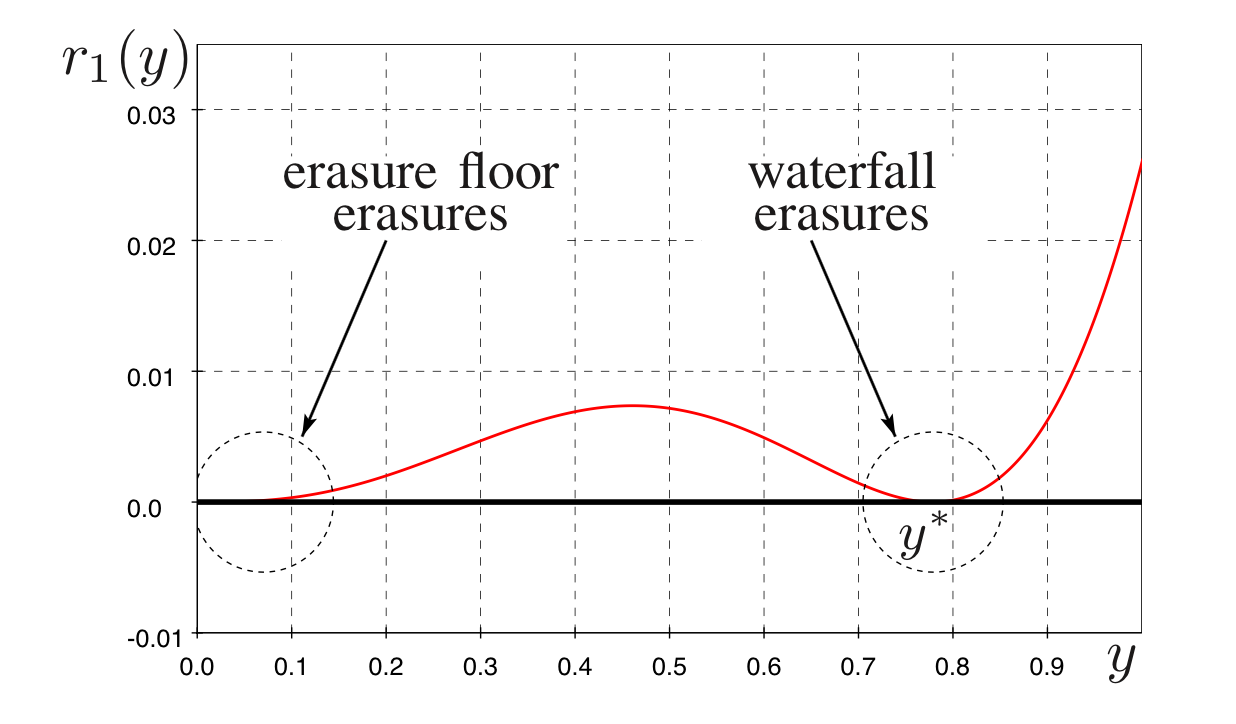
\includegraphics[width=0.85\textwidth]{data/UMAC/Figures/small_large_Erasures.png}
\caption{$\tilde{R}_{1}(y)$ at $\epsilon=\epsilon_{\text{BP}}$ for $\lmb(x)=x^2,\rho(x)=x^5$. Note that this figure is reproduced from \cite{amraoui2007find}.}
\label{Fig:LDPCResidual}
\end{figure}

\subsection{Error probability approximates}
 The authors \cite{amraoui2007find} demonstrate that (can also be observed from Fig. \ref{Fig:LDPCResidual}) the failure of decoder occurs with high probability in two possible scenarios: The first case corresponds to $y\approx 0$ or as $t\rightarrow \infty$ and the other case corresponds to the value of $y$ such that $\tilde{R}_{1}(y)=0$ when $\epsilon=\epsilon_{\text{BP}}$ or equivalently at the value of $y$ where the curve has a stationary point. This point is referred to as critical point $y^*.$ The errors caused corresponding to the first case are referred to as \textit{small-error} events or error floor erasures since they occur towards the end of peeling decoder and the errors corresponding to the second case are referred to as \textit{large-error} events or waterfall erasures. The authors approximate the total probability of error by two expressions, each one corresponding to the one of these two cases.
 
%\subsubsection*{LP to increase the net throughput}~\\ \\ $\max \frac{-(1-P_b)}{m^2}\Delta m+\sum_{i}-\frac{\partial P_b•}{m\partial L_i}\Delta L_i- \frac{~\partial P_b}{m\partial m}\Delta m$
%\begin{align*}
%&\sum \Delta L_i=0;      & -\min\{\delta,L_{i}\}\leq \Delta L_i\leq \delta
%\end{align*}

\begin{theorem}[Scaling Law \cite{richardson2008modern}]
Consider transmission over a BEC channel using random elements from the LDPC $(n,\lambda,\rho)$ ensemble. Assume that the ensemble has a single critical point $y^*>0$ and let $\nu^*=\epsilon_{\text{BP}}L(y^*)$. Let $P_{\text{B}}^{W}(n,\lmb,\rho,\epsilon)$ denote the expected block erasure probability due to erasures of size atleast $n\gamma \nu^{*}$, where $\gamma\in (0,1)$. Fix $z:=\sqrt{n}(\epsilon_{\text{BP}}-\beta n^{-2/3}-\epsilon)$. Then as $n\rightarrow \infty ,$
\begin{align*}
P_{\text{B}}^{W}(n,\lmb,\rho,\epsilon)=Q\left(\frac{z}{\alpha}\right)\left(1+O(n^{-1/3})\right)
\end{align*}
where $\alpha$ and $\beta$ are constants dependent on the degree distributions.
\end{theorem}
The expression above approximates the error probability of large-erasure events.

\begin{theorem}[Error Floor \cite{amraoui2007find}]
Consider transmission over a BEC channel using random elements from the LDPC $(n,\lambda,\rho)$ ensemble. Assume that the ensemble has a single critical point $y^*>0$ and let $\nu^*=\epsilon_{\text{BP}}L(y^*)$. Let $P_{\text{B}}^{F}(n,\lmb,\rho,\epsilon)$ denote the expected block erasure probability due to stopping sets of size between $s_{\text{min}}$ and  $n\gamma \nu^{*}$, where $\gamma\in (0,1)$. Then for any $\epsilon<\epsilon_{\text{BP}}$
\begin{align*}
P_{\text{B}}^{F}(n,\lmb,\rho,\epsilon)=1-e^{-\sum_{s\geq s_{min}}\tilde{A}_{s}\epsilon^s}\left(1+o(1)\right),
\end{align*}
where $\tilde{A}_{s}=\text{coef}\{\log(A(x)),x^s\}$ for $s\geq 1$, with $A(x)=\sum_{s\geq 0} A_{s}x^s$ and
\begin{multline}
A_{s}=\sum_{e}\left( \text{coef}\left\lbrace\prod_{i} (1+xy^{i})^{nL_{i}}, x^{s}y^{e} \right\rbrace \right.\times \\
\left.\frac{\text{coef}\lbrace \prod_{i}\left((1+x)^i -ix \right)^{n(1-r)R_{i}},x^{e}\rbrace}{\binom{nL'(1)}{e}}\right).
\end{multline}
\end{theorem}
Note that $A_{s}$ is the expected number of stopping sets of size $s$ in a random graph picked uniformly at random from the graph and $\tilde{A}_{s}$ is the expected number of minimal stopping sets of size $s$. Following along similar lines we derive error floor expression in the case of random multiple access problem.
 
%Our objective is, for a given $n$, to minimize the total throughput $\eta=\frac{n}{m}\left(1-P_{b}(n,L(x)\right)$ over the variables $m$-number of slots and the degree distribution $L(x)$. Even from the analytical approximate expression for the bit/block probability of error it appears to be a highly complex problem and the global optimization would be very difficult to compute. So for a fixed $n$ and an initial left distribution $L(x)$ we compute the partial derivatives and implement the local optimization via LP to derive a locally optimal left distribution $L^{*}(x)$. With this as our current input to the LP we repeat the procedure until there are diminishing improvements to the total throughput $\eta$.

\section{Error analysis for random multiple access}
  We note that in the case of random uncoordinated multiple access scheme since the right degree distribution is not a design choice but rather has a Poisson distribution, as discussed in \cite{narayanan2012iterative}, the error probability approximations do not carry over directly from \cite{amraoui2007find} especially for the \textit{water-fall} erasures. But we approximate the small-error events $P_{\text{b}}^{\text{F}}(n,L)$, where `F' stands for error floor, the expression for which is given in \ref{sec:UMACapproximate}. We avoid the large error events by imposing a constraint in the optimization problem that the residual degree-1 check nodes $\tilde{R}_1(y)$ in the initial stages of peeling decoder is bounded away from $0$ by a certain threshold and thus the overall probability of error is well approximated by $P_{\text{b}}^{\text{F}}(n,L)$ alone. We support this claim by providing evidence via simulations.

%We consider the paradigm in which $k^{\text{th}}$ user/bit-node, for $k\in [1:n]$, generates a random variable $D_{k}$ from the probability mass function $L(x)$ independent of other bit nodes or equivalently $\text{Pr}(D_{k}=i)=L_{i}$. Each bit node, after the generation of $D_{k}$, chooses $D_{k}$ time slots/check nodes uniformly at random, with replacement, from the $m$ check nodes available. 

We will refer to the random access paradigm of picking check nodes randomly but with replacement as \textit{uniform-with replacement} paradigm. Even though the ``uniform-with replacement" allows for multiple edges in the graph, the analysis is made easier because of this assumption. For a given edge, probability that it connects to any of the check nodes is equal to $\frac{1}{m}$. We also believe that the resulting analysis can be easily extended to the ``uniform-without replacement" paradigm where in the $D_{k}$ check nodes are picked uniformly at random, but without replacement from the $m$ check nodes. Note that in Narayanan, Pfister \cite{narayanan2012iterative} consider the `` uniform-without replacement" paradigm. We define the ensemble of graphs for the random multiple access problem as UMAC$(n,\lmb,\eta)$ where $L(x)$ is as described in Eqn.~\eqref{eqn:varnodedd_LDPC}, is related to $\lmb(x)$ via
\begin{align*}
L(x)=\frac{\int_{0}^{x}\lmb(x)}{\int_{0}^{1}\lmb(x)}.
\end{align*}
 $\eta$ is the throughput ($n=m\eta$) and the edges are chosen as in the ``uniform-without replacement" paradigm.

\subsection{Error Probability approximates}
\label{sec:UMACapproximate}
\begin{theorem}[Small error events]
Consider transmission by users over a noiseless MAC channel according to a graph picked uniformly at random from the UMAC$(n,\lmb,\eta)$ ensemble. Assume that the ensemble has no critical point i.e the degree-one check nodes in the residual graph is a monotonously decreasing function of time. Let $P_{\text{B},s_{min}}^{F}(n,\lmb,\rho,\epsilon)$ denote the expected block erasure probability due to stopping sets of size between $s_{min}$ and  $\gamma n$, where $\gamma\in (0,1)$. Then
\begin{align}
P_{\text{B},s_{min}}^{F}(n,\lmb,\rho,\epsilon)=1-e^{-\sum\limits_{s\geq s_{\text{min}}}^{\gamma n}\tilde{A}_{s}}\left(1+o(1)\right),
\label{Eqn:PBAnalytic}
\end{align}
where $\tilde{A}_{s}=\text{coef}\{\log(A(x)),x^s\}$ for $s\geq 1$, with $A(x)=\sum_{s\geq 0} A_{s}x^s$ and
\begin{multline}\label{Eqn:AvgSS}
A_{s}=\sum_{i}\left(\text{coef}\left\lbrace (1+x\sum_{i}L_{i}y^{i})^{n}, x^{s}y^{i} \right\rbrace \right.\times \\
\left.\frac{\text{coef}\lbrace (e^x -x)^{m},x^{i}\rbrace }{\frac{m^i}{i!}}\right). \\
\end{multline}
\label{Thm:UMACFloor}
\end{theorem}

\begin{proof}
We now give only a brief glimpse of the proof, the detailed proof will be added later. We first show that the expression for $A_{s}$ in \eqref{Eqn:AvgSS} is equal to the expected number of stopping sets of size `$s$' in a graph picked uniformly at random from the UMAC($n,\lmb,\eta$) ensemble. The first term is $\binom{n}{s}$ times the probability that $s$ nodes have $e$ edges attached to them and the second term is equal to the probability that the $e$ edges, under the ``uniform-with replacement" paradigm, form a stopping set i.e, they choose check nodes such that none of the check nodes chosen have only one edge connection.

From there we will try to follow the similar argument as in \cite{richardson2008modern} that for large values of $n$ the minimal stopping sets tend to a Poisson distribution with independent components. And then the relation between $A(x)$ and $\tilde{A}(x)$, expression for block/bit error probability follows along the same lines.
\end{proof}

\begin{remark}
Even though the condition in Theorem \ref{Thm:UMACFloor} that the degree-1 check nodes in the residual graph decrease monotonously with time is a stringent constraint to be satisfied, we believe that even when the curve of degree-1 check nodes has a stationary  point (curve $\tilde{R}_{1}(y)$ is non-monotonous function of $y$) the expression in Eqn. \eqref{Eqn:AvgSS}  approximates the probability of small error events well enough.
\end{remark}

\subsection{Results}
We use the following degree distribution, with a maximum degree of 30. Note that we chose this distribution randomly.
\begin{multline}
L_1(x)=0.3x^2+ 0.25 x^3+ 0.2 x^4 + 0.1 x^5+ 0.05 x^{10} + 0.04 x^{15}\\
 + 0.03 x^{20} + 0.02 x^{25}+ 0.01 x^{30}.
\label{Eqn:L1x}
\end{multline}
For the parameters of $n=1000, m=1300( \eta \approx 0.77)$ and $L(x)$ in Eqn. \eqref{Eqn:L1x} we get the following results given in Table.~\ref{Table:SimvsAnalytic1}. Note that $P_{B,s_{\text{min}}}^F$ is computed using the analytic expression given in \eqref{Eqn:PBAnalytic} whereas $P_{B,s_{\text{min}}}^{\text{Sim}}$ is computed using numeric simulations of Peeling decoder.


\begin{figure}
\centering
\setlength\figurewidth{0.8\columnwidth}
\setlength\figureheight{0.6\columnwidth}
% This file was created by matlab2tikz v0.4.7 running on MATLAB 7.14.
% Copyright (c) 2008--2014, Nico Schlömer <nico.schloemer@gmail.com>
% All rights reserved.
% Minimal pgfplots version: 1.3
% 
% The latest updates can be retrieved from
%   http://www.mathworks.com/matlabcentral/fileexchange/22022-matlab2tikz
% where you can also make suggestions and rate matlab2tikz.
% 
\begin{tikzpicture}

\begin{axis}[%
width=\figurewidth,
height=\figureheight,
scale only axis,
xmin=0,
xmax=1,
xlabel={Iterations},
xmajorgrids,
ymin=-40,
ymax=200,
ylabel={Residual Degree-1 Check Nodes},
ymajorgrids,
legend style={at={(0,1)},anchor=north west,draw=black,fill=white,legend cell align=left}
]
\addplot [color=red,solid,line width=1.5pt]
  table[row sep=crcr]{0	0\\
0.01	0.0324342999246084\\
0.02	0.130205815361465\\
0.03	0.293987817090611\\
0.04	0.524410156505397\\
0.05	0.822054268200592\\
0.06	1.18744801438634\\
0.07	1.62106039064647\\
0.08	2.12329611484881\\
0.09	2.69449012337941\\
0.1	3.33490200129503\\
0.11	4.0447103754538\\
0.12	4.8240073021706\\
0.13	5.67279268342755\\
0.14	6.59096874812536\\
0.15	7.57833463725704\\
0.16	8.63458113419017\\
0.17	9.7592855834234\\
0.18	10.951907043196\\
0.19	12.2117817191437\\
0.2	13.5381187277618\\
0.21	14.9299962397182\\
0.22	16.3863580540202\\
0.23	17.9060106546155\\
0.24	19.4876208011846\\
0.25	21.1297137055917\\
0.26	22.8306718446789\\
0.27	24.5887344587651\\
0.28	26.4019977833131\\
0.29	28.2684160587129\\
0.3	30.1858033599693\\
0.31	32.1518362842367\\
0.32	34.164057529585\\
0.33	36.219880393077\\
0.34	38.3165942101612\\
0.35	40.4513707504974\\
0.36	42.6212715776194\\
0.37	44.823256371239\\
0.38	47.0541922015086\\
0.39	49.3108637340943\\
0.4	51.5899843334615\\
0.41	53.8882080192293\\
0.42	56.202142216772\\
0.43	58.5283612282931\\
0.44	60.8634203342801\\
0.45	63.2038704173866\\
0.46	65.5462729812106\\
0.47	67.8872154148936\\
0.48	70.2233263306744\\
0.49	72.5512907751393\\
0.5	74.8678650854909\\
0.51	77.1698911291758\\
0.52	79.4543096280644\\
0.53	81.7181722262746\\
0.54	83.9586519127884\\
0.55	86.1730513551339\\
0.56	88.3588086372915\\
0.57	90.5134998221086\\
0.58	92.6348376740633\\
0.59	94.720665780088\\
0.6	96.7689471918946\\
0.61	98.7777465800384\\
0.62	100.745204734634\\
0.63	102.669504066718\\
0.64	104.548823553981\\
0.65	106.381281331209\\
0.66	108.164862845722\\
0.67	109.897332178663\\
0.68	111.576123773185\\
0.69	113.198211412465\\
0.7	114.759950861394\\
0.71	116.256892141816\\
0.72	117.683556981988\\
0.73	119.033176617602\\
0.74	120.297384908265\\
0.75	121.465861803666\\
0.76	122.525922757217\\
0.77	123.462051063987\\
0.78	124.255372784973\\
0.79	124.883078650327\\
0.8	125.317805215192\\
0.81	125.527000210276\\
0.82	125.472316889248\\
0.83	125.109112717954\\
0.84	124.386173978577\\
0.85	123.245856810552\\
0.86	121.624936521538\\
0.87	119.456603397797\\
0.88	116.674250532317\\
0.89	113.217985052458\\
0.9	109.045174254886\\
0.91	104.146817251678\\
0.92	98.5720866215064\\
0.93	92.4639285313235\\
0.94	86.108949459999\\
0.95	80.004586182306\\
0.96	74.9451636677844\\
0.97	72.125118791915\\
0.98	73.2517287294828\\
0.99	80.6513121779363\\
1	97.3445263373793\\
};
\addlegendentry{$L_1(x),\eta=0.77$};

\addplot [color=blue,solid,line width=1.5pt]
  table[row sep=crcr]{0	-0\\
0.01	0.0324342999454241\\
0.02	0.130205816540216\\
0.03	0.293987828713633\\
0.04	0.524410211361817\\
0.05	0.822054436379727\\
0.06	1.18744839020242\\
0.07	1.62106101023381\\
0.08	2.12329674311493\\
0.09	2.69448982841213\\
0.1	3.33489841199594\\
0.11	4.04469849414493\\
0.12	4.82397771825418\\
0.13	5.67272900696705\\
0.14	6.59084405359321\\
0.15	7.57810667783715\\
0.16	8.63418605615414\\
0.17	9.7586298384885\\
0.18	10.9508571647491\\
0.19	12.2101515961551\\
0.2	13.5356539785588\\
0.21	14.9263552570484\\
0.22	16.3810892635637\\
0.23	17.8985255019548\\
0.24	19.4771619579028\\
0.25	21.1153179644249\\
0.26	22.8111271573443\\
0.27	24.5625305591447\\
0.28	26.3672698340911\\
0.29	28.2228807624179\\
0.3	30.1266869868122\\
0.31	32.0757940903889\\
0.32	34.0670840719254\\
0.33	36.0972102913402\\
0.34	38.1625929663138\\
0.35	40.2594153096284\\
0.36	42.3836204062868\\
0.37	44.53090893983\\
0.38	46.6967378885548\\
0.39	48.8763203246001\\
0.4	51.0646264621615\\
0.41	53.256386115464\\
0.42	55.4460927425935\\
0.43	57.6280092678901\\
0.44	59.7961758933262\\
0.45	61.9444201281343\\
0.46	64.0663692858302\\
0.47	66.155465718642\\
0.48	68.2049850810613\\
0.49	70.2080579365958\\
0.5	72.1576950445935\\
0.51	74.0468166869157\\
0.52	75.8682864168572\\
0.53	77.6149496345894\\
0.54	79.2796774139531\\
0.55	80.8554160239703\\
0.56	82.3352426042164\\
0.57	83.7124274653064\\
0.58	84.9805034932132\\
0.59	86.1333431379365\\
0.6	87.1652434620313\\
0.61	88.0710197116236\\
0.62	88.8461078507147\\
0.63	89.4866764678907\\
0.64	89.9897484223778\\
0.65	90.3533325433943\\
0.66	90.5765656332882\\
0.67	90.6598649520345\\
0.68	90.6050912804597\\
0.69	90.4157225754979\\
0.7	90.0970381480775\\
0.71	89.6563132202427\\
0.72	89.1030236627827\\
0.73	88.4490606911378\\
0.74	87.7089553225666\\
0.75	86.9001124927707\\
0.76	86.0430549217833\\
0.77	85.1616771389922\\
0.78	84.2835105643373\\
0.79	83.4400012426543\\
0.8	82.6668027943376\\
0.81	82.0040884396886\\
0.82	81.4968876468592\\
0.83	81.1954551232481\\
0.84	81.1556826049878\\
0.85	81.4395672936855\\
0.86	82.1157549444023\\
0.87	83.2601806270451\\
0.88	84.9568361654408\\
0.89	87.2987002943643\\
0.9	90.3888757323577\\
0.91	94.3419866749835\\
0.92	99.285900631951\\
0.93	105.363849925412\\
0.94	112.73704025256\\
0.95	121.587846004979\\
0.96	132.123703765158\\
0.97	144.581825449799\\
0.98	159.234859404874\\
0.99	176.397629401307\\
1	196.435075586923\\
};
\addlegendentry{$L_2(x),\eta=0.77$};

\addplot [color=green,solid,line width=1.5pt]
  table[row sep=crcr]{0	0\\
0.01	0.0258363854806183\\
0.02	0.10328147936136\\
0.03	0.232180465548624\\
0.04	0.412295746914854\\
0.05	0.643301284286838\\
0.06	0.924776895131598\\
0.07	1.25620254462867\\
0.08	1.63695266473375\\
0.09	2.06629053978564\\
0.1	2.54336280015728\\
0.11	3.06719406837351\\
0.12	3.63668180497762\\
0.13	4.25059140418947\\
0.14	4.90755159201914\\
0.15	5.60605018193617\\
0.16	6.34443024540351\\
0.17	7.12088675651487\\
0.18	7.93346377157502\\
0.19	8.78005220569002\\
0.2	9.65838826922263\\
0.21	10.566052627285\\
0.22	11.5004703452196\\
0.23	12.4589116822184\\
0.24	13.4384937938054\\
0.25	14.4361834018069\\
0.26	15.448800487628\\
0.27	16.4730230610944\\
0.28	17.5053930527862\\
0.29	18.5423233726491\\
0.3	19.5801061716993\\
0.31	20.6149223368319\\
0.32	21.6428522410704\\
0.33	22.659887763072\\
0.34	23.6619455803104\\
0.35	24.6448817300991\\
0.36	25.6045074215048\\
0.37	26.5366060692219\\
0.38	27.4369515076605\\
0.39	28.3013273298053\\
0.4	29.1255472808813\\
0.41	29.9054766214382\\
0.42	30.6370543581812\\
0.43	31.316316223638\\
0.44	31.9394182675541\\
0.45	32.5026609036361\\
0.46	33.0025132348499\\
0.47	33.4356374587621\\
0.48	33.7989131312368\\
0.49	34.0894610419457\\
0.5	34.3046664283566\\
0.51	34.4422012257884\\
0.52	34.5000450194179\\
0.53	34.4765043292729\\
0.54	34.3702298207703\\
0.55	34.1802309905898\\
0.56	33.9058878299362\\
0.57	33.5469589137436\\
0.58	33.1035853042668\\
0.59	32.5762895899212\\
0.6	31.9659693043004\\
0.61	31.273883885283\\
0.62	30.5016342395385\\
0.63	29.6511338735247\\
0.64	28.7245704390083\\
0.65	27.7243564213245\\
0.66	26.6530675760932\\
0.67	25.5133676021811\\
0.68	24.3079174371861\\
0.69	23.0392674954878\\
0.7	21.7097311669398\\
0.71	20.3212380004924\\
0.72	18.8751652768365\\
0.73	17.3721472239657\\
0.74	15.8118620902465\\
0.75	14.1927988652998\\
0.76	12.5120079237899\\
0.77	10.7648436817441\\
0.78	8.94471309749036\\
0.79	7.04285236422604\\
0.8	5.04816661144334\\
0.81	2.94718549755974\\
0.82	0.72421347887326\\
0.83	-1.63820970755115\\
0.84	-4.15837126603556\\
0.85	-6.85373189389589\\
0.86	-9.73822137652723\\
0.87	-12.8180192202839\\
0.88	-16.0851907616107\\
0.89	-19.5083461089709\\
0.9	-23.0192582796967\\
0.91	-26.4941480676831\\
0.92	-29.7281825415224\\
0.93	-32.4017635113411\\
0.94	-34.0375972213806\\
0.95	-33.9486014601399\\
0.96	-31.1786855215329\\
0.97	-24.4413895725551\\
0.98	-12.0647201528052\\
0.99	8.04756732743722\\
1	38.4311186492295\\
};
\addlegendentry{$L_1(x),\eta=0.95$};

\end{axis}
\end{tikzpicture}%
\caption{$\tilde{R}_{1}(y)$ for UMAC($1000,L(x),0.77$) corresponding to $L_{1,2}(x)$ in Eqn. \eqref{Eqn:L1x}.}
\label{Fig:UMAC_Residual}
\end{figure}

\begin{table}
\centering
\begin{tabular}{c c c c c}
\hline  \hline
smin & $P_{B,\text{smin}}^F$ & $P_{B,\text{smin}}^{\text{Sim}}$ & $P_{b,\text{smin}}^F$ & $P_{b,\text{smin}}^{\text{Sim}}$ \\
\hline
2 & 7.89$\times 10^{-2}$  &  7.97$\times 10^{-2}$ &$2.13\times 10^{-4}$&$2.12\times 10^{-4}$\\
3 & 2.78$\times 10^{-2}$  & 2.84$\times 10^{-2}$&$1.05\times 10^{-4}$&$1.09\times 10^{-4}$ \\
4 & 1.11$\times 10^{-2}$  &1.30$\times 10^{-2}$ &$5.41\times 10^{-5}$&$6.33\times 10^{-5}$\\
5 & 4.80$\times 10^{-3}$  &5.90$\times 10^{-3}$& $2.88\times 10^{-5}$&$3.49\times 10^{-5}$\\
6 & 2.23$\times 10^{-3}$  &3.00$\times 10^{-3}$ &$1.58\times 10^{-5}$&$2.04\times 10^{-5}$\\
7 & 1.10$\times 10^{-3}$  &1.50$\times 10^{-3}$ &$9.04\times 10^{-6}$&$1.14\times 10^{-5}$\\
8 &5.68$\times 10^{-4}$   &5.00$\times 10^{-3}$&$5.28\times 10^{-6}$&$4.40\times 10^{-6}$\\
9 & 3.03$\times 10^{-4}$  &3.00$\times 10^{-4}$ & $3.15\times 10^{-6}$&$2.80\times 10^{-6}$\\
10 & 1.66$\times 10^{-4}$ &1.00$\times 10^{-4}$&$1.90\times 10^{-6}$&$1.00\times 10^{-6}$\\
\end{tabular}
\caption{Comparison of Probability of Block\textbackslash Bit errors computed analytically and via simulations for $L_1(x)$ given by Eqn. \eqref{Eqn:L1x}, $K=1000, \eta=0.77$.}
\label{Table:SimvsAnalytic1}
\end{table}

We notice that the analytic and numerical results are almost in perfect agreement. To justify applying Thm. \ref{Thm:UMACFloor} we verify that most of the error events are of small size, analytically through Fig.~\ref{Fig:UMAC_Residual}. We also verify numerically that the maximum stopping set size we observe is 22 thus rendering an approximation for error probability because of large error events unnecessary. \\

To verify for another distribution, we perform the experiments for another bit-node distribution given in Eqn. \eqref{Eqn:L2x}. The evolution of residual degree-1 check nodes is given in Fig. \ref{Fig:UMAC_Residual}. The corresponding numeric results obtained via simulations are given in Table. \ref{Table:SimvsAnalytic2}.
\begin{multline}
L_{2}(x)=0.3x^2+ 0.25 x^3+ 0.2 x^4 + 0.1 x^5+ 0.05 x^{6} + 0.04 x^{7}\\
 + 0.03 x^{8} + 0.02 x^{10}+ 0.01 x^{20}.
\label{Eqn:L2x}
\end{multline}

%\begin{figure}
%\centering
%\setlength\figurewidth{0.8\columnwidth}
%\setlength\figureheight{0.6\columnwidth}
%% This file was created by matlab2tikz v0.4.7 running on MATLAB 7.14.
% Copyright (c) 2008--2014, Nico Schlömer <nico.schloemer@gmail.com>
% All rights reserved.
% Minimal pgfplots version: 1.3
% 
% The latest updates can be retrieved from
%   http://www.mathworks.com/matlabcentral/fileexchange/22022-matlab2tikz
% where you can also make suggestions and rate matlab2tikz.
% 
\begin{tikzpicture}

\begin{axis}[%
width=\figurewidth,
height=\figureheight,
scale only axis,
xmin=0,
xmax=1,
xlabel={Iterations},
xmajorgrids,
ymin=-40,
ymax=200,
ylabel={Residual Degree-1 Check Nodes},
ymajorgrids,
legend style={at={(0,1)},anchor=north west,draw=black,fill=white,legend cell align=left}
]
\addplot [color=red,solid,line width=1.5pt]
  table[row sep=crcr]{0	0\\
0.01	0.0324342999246084\\
0.02	0.130205815361465\\
0.03	0.293987817090611\\
0.04	0.524410156505397\\
0.05	0.822054268200592\\
0.06	1.18744801438634\\
0.07	1.62106039064647\\
0.08	2.12329611484881\\
0.09	2.69449012337941\\
0.1	3.33490200129503\\
0.11	4.0447103754538\\
0.12	4.8240073021706\\
0.13	5.67279268342755\\
0.14	6.59096874812536\\
0.15	7.57833463725704\\
0.16	8.63458113419017\\
0.17	9.7592855834234\\
0.18	10.951907043196\\
0.19	12.2117817191437\\
0.2	13.5381187277618\\
0.21	14.9299962397182\\
0.22	16.3863580540202\\
0.23	17.9060106546155\\
0.24	19.4876208011846\\
0.25	21.1297137055917\\
0.26	22.8306718446789\\
0.27	24.5887344587651\\
0.28	26.4019977833131\\
0.29	28.2684160587129\\
0.3	30.1858033599693\\
0.31	32.1518362842367\\
0.32	34.164057529585\\
0.33	36.219880393077\\
0.34	38.3165942101612\\
0.35	40.4513707504974\\
0.36	42.6212715776194\\
0.37	44.823256371239\\
0.38	47.0541922015086\\
0.39	49.3108637340943\\
0.4	51.5899843334615\\
0.41	53.8882080192293\\
0.42	56.202142216772\\
0.43	58.5283612282931\\
0.44	60.8634203342801\\
0.45	63.2038704173866\\
0.46	65.5462729812106\\
0.47	67.8872154148936\\
0.48	70.2233263306744\\
0.49	72.5512907751393\\
0.5	74.8678650854909\\
0.51	77.1698911291758\\
0.52	79.4543096280644\\
0.53	81.7181722262746\\
0.54	83.9586519127884\\
0.55	86.1730513551339\\
0.56	88.3588086372915\\
0.57	90.5134998221086\\
0.58	92.6348376740633\\
0.59	94.720665780088\\
0.6	96.7689471918946\\
0.61	98.7777465800384\\
0.62	100.745204734634\\
0.63	102.669504066718\\
0.64	104.548823553981\\
0.65	106.381281331209\\
0.66	108.164862845722\\
0.67	109.897332178663\\
0.68	111.576123773185\\
0.69	113.198211412465\\
0.7	114.759950861394\\
0.71	116.256892141816\\
0.72	117.683556981988\\
0.73	119.033176617602\\
0.74	120.297384908265\\
0.75	121.465861803666\\
0.76	122.525922757217\\
0.77	123.462051063987\\
0.78	124.255372784973\\
0.79	124.883078650327\\
0.8	125.317805215192\\
0.81	125.527000210276\\
0.82	125.472316889248\\
0.83	125.109112717954\\
0.84	124.386173978577\\
0.85	123.245856810552\\
0.86	121.624936521538\\
0.87	119.456603397797\\
0.88	116.674250532317\\
0.89	113.217985052458\\
0.9	109.045174254886\\
0.91	104.146817251678\\
0.92	98.5720866215064\\
0.93	92.4639285313235\\
0.94	86.108949459999\\
0.95	80.004586182306\\
0.96	74.9451636677844\\
0.97	72.125118791915\\
0.98	73.2517287294828\\
0.99	80.6513121779363\\
1	97.3445263373793\\
};
\addlegendentry{$L_1(x),\eta=0.77$};

\addplot [color=blue,solid,line width=1.5pt]
  table[row sep=crcr]{0	-0\\
0.01	0.0324342999454241\\
0.02	0.130205816540216\\
0.03	0.293987828713633\\
0.04	0.524410211361817\\
0.05	0.822054436379727\\
0.06	1.18744839020242\\
0.07	1.62106101023381\\
0.08	2.12329674311493\\
0.09	2.69448982841213\\
0.1	3.33489841199594\\
0.11	4.04469849414493\\
0.12	4.82397771825418\\
0.13	5.67272900696705\\
0.14	6.59084405359321\\
0.15	7.57810667783715\\
0.16	8.63418605615414\\
0.17	9.7586298384885\\
0.18	10.9508571647491\\
0.19	12.2101515961551\\
0.2	13.5356539785588\\
0.21	14.9263552570484\\
0.22	16.3810892635637\\
0.23	17.8985255019548\\
0.24	19.4771619579028\\
0.25	21.1153179644249\\
0.26	22.8111271573443\\
0.27	24.5625305591447\\
0.28	26.3672698340911\\
0.29	28.2228807624179\\
0.3	30.1266869868122\\
0.31	32.0757940903889\\
0.32	34.0670840719254\\
0.33	36.0972102913402\\
0.34	38.1625929663138\\
0.35	40.2594153096284\\
0.36	42.3836204062868\\
0.37	44.53090893983\\
0.38	46.6967378885548\\
0.39	48.8763203246001\\
0.4	51.0646264621615\\
0.41	53.256386115464\\
0.42	55.4460927425935\\
0.43	57.6280092678901\\
0.44	59.7961758933262\\
0.45	61.9444201281343\\
0.46	64.0663692858302\\
0.47	66.155465718642\\
0.48	68.2049850810613\\
0.49	70.2080579365958\\
0.5	72.1576950445935\\
0.51	74.0468166869157\\
0.52	75.8682864168572\\
0.53	77.6149496345894\\
0.54	79.2796774139531\\
0.55	80.8554160239703\\
0.56	82.3352426042164\\
0.57	83.7124274653064\\
0.58	84.9805034932132\\
0.59	86.1333431379365\\
0.6	87.1652434620313\\
0.61	88.0710197116236\\
0.62	88.8461078507147\\
0.63	89.4866764678907\\
0.64	89.9897484223778\\
0.65	90.3533325433943\\
0.66	90.5765656332882\\
0.67	90.6598649520345\\
0.68	90.6050912804597\\
0.69	90.4157225754979\\
0.7	90.0970381480775\\
0.71	89.6563132202427\\
0.72	89.1030236627827\\
0.73	88.4490606911378\\
0.74	87.7089553225666\\
0.75	86.9001124927707\\
0.76	86.0430549217833\\
0.77	85.1616771389922\\
0.78	84.2835105643373\\
0.79	83.4400012426543\\
0.8	82.6668027943376\\
0.81	82.0040884396886\\
0.82	81.4968876468592\\
0.83	81.1954551232481\\
0.84	81.1556826049878\\
0.85	81.4395672936855\\
0.86	82.1157549444023\\
0.87	83.2601806270451\\
0.88	84.9568361654408\\
0.89	87.2987002943643\\
0.9	90.3888757323577\\
0.91	94.3419866749835\\
0.92	99.285900631951\\
0.93	105.363849925412\\
0.94	112.73704025256\\
0.95	121.587846004979\\
0.96	132.123703765158\\
0.97	144.581825449799\\
0.98	159.234859404874\\
0.99	176.397629401307\\
1	196.435075586923\\
};
\addlegendentry{$L_2(x),\eta=0.77$};

\addplot [color=green,solid,line width=1.5pt]
  table[row sep=crcr]{0	0\\
0.01	0.0258363854806183\\
0.02	0.10328147936136\\
0.03	0.232180465548624\\
0.04	0.412295746914854\\
0.05	0.643301284286838\\
0.06	0.924776895131598\\
0.07	1.25620254462867\\
0.08	1.63695266473375\\
0.09	2.06629053978564\\
0.1	2.54336280015728\\
0.11	3.06719406837351\\
0.12	3.63668180497762\\
0.13	4.25059140418947\\
0.14	4.90755159201914\\
0.15	5.60605018193617\\
0.16	6.34443024540351\\
0.17	7.12088675651487\\
0.18	7.93346377157502\\
0.19	8.78005220569002\\
0.2	9.65838826922263\\
0.21	10.566052627285\\
0.22	11.5004703452196\\
0.23	12.4589116822184\\
0.24	13.4384937938054\\
0.25	14.4361834018069\\
0.26	15.448800487628\\
0.27	16.4730230610944\\
0.28	17.5053930527862\\
0.29	18.5423233726491\\
0.3	19.5801061716993\\
0.31	20.6149223368319\\
0.32	21.6428522410704\\
0.33	22.659887763072\\
0.34	23.6619455803104\\
0.35	24.6448817300991\\
0.36	25.6045074215048\\
0.37	26.5366060692219\\
0.38	27.4369515076605\\
0.39	28.3013273298053\\
0.4	29.1255472808813\\
0.41	29.9054766214382\\
0.42	30.6370543581812\\
0.43	31.316316223638\\
0.44	31.9394182675541\\
0.45	32.5026609036361\\
0.46	33.0025132348499\\
0.47	33.4356374587621\\
0.48	33.7989131312368\\
0.49	34.0894610419457\\
0.5	34.3046664283566\\
0.51	34.4422012257884\\
0.52	34.5000450194179\\
0.53	34.4765043292729\\
0.54	34.3702298207703\\
0.55	34.1802309905898\\
0.56	33.9058878299362\\
0.57	33.5469589137436\\
0.58	33.1035853042668\\
0.59	32.5762895899212\\
0.6	31.9659693043004\\
0.61	31.273883885283\\
0.62	30.5016342395385\\
0.63	29.6511338735247\\
0.64	28.7245704390083\\
0.65	27.7243564213245\\
0.66	26.6530675760932\\
0.67	25.5133676021811\\
0.68	24.3079174371861\\
0.69	23.0392674954878\\
0.7	21.7097311669398\\
0.71	20.3212380004924\\
0.72	18.8751652768365\\
0.73	17.3721472239657\\
0.74	15.8118620902465\\
0.75	14.1927988652998\\
0.76	12.5120079237899\\
0.77	10.7648436817441\\
0.78	8.94471309749036\\
0.79	7.04285236422604\\
0.8	5.04816661144334\\
0.81	2.94718549755974\\
0.82	0.72421347887326\\
0.83	-1.63820970755115\\
0.84	-4.15837126603556\\
0.85	-6.85373189389589\\
0.86	-9.73822137652723\\
0.87	-12.8180192202839\\
0.88	-16.0851907616107\\
0.89	-19.5083461089709\\
0.9	-23.0192582796967\\
0.91	-26.4941480676831\\
0.92	-29.7281825415224\\
0.93	-32.4017635113411\\
0.94	-34.0375972213806\\
0.95	-33.9486014601399\\
0.96	-31.1786855215329\\
0.97	-24.4413895725551\\
0.98	-12.0647201528052\\
0.99	8.04756732743722\\
1	38.4311186492295\\
};
\addlegendentry{$L_1(x),\eta=0.95$};

\end{axis}
\end{tikzpicture}%
%\caption{$\tilde{R}_{1}(y)$ for UMAC($1000,L(x),0.77$) corresponding to $L(x)$ in Eqn. \eqref{Eqn:L2x}.}
%\label{Fig:UMAC_Residual_NonMonotonous2}
%\end{figure}

\begin{table}
\centering
\begin{tabular}{c c c c c}
\hline  \hline
smin & $P_{B,s_{\text{min}}}^F$ & $P_{B,s_{\text{min}}}^{\text{Sim}}$& $P_{b,\text{smin}}^F$ & $P_{b,\text{smin}}^{\text{Sim}}$ \\
\hline
2 & 7.91$\times 10^{-2}$  &7.67$\times 10^{-2}$ &$2.13\times 10^{-4}$&$2.08\times 10^{-4}$\\
3 & 2.79$\times 10^{-2}$  &2.86$\times 10^{-2}$&$1.05\times 10^{-4}$&$1.12\times 10^{-4}$ \\
4 & 1.11$\times 10^{-2}$  &1.28$\times 10^{-2}$ &$5.41\times 10^{-5}$&$6.49\times 10^{-5}$\\
5 & 4.82$\times 10^{-3}$  &6.43$\times 10^{-3}$ & $2.88\times 10^{-5}$&$3.94\times 10^{-5}$\\
6 & 2.25$\times 10^{-3}$  &3.56$\times 10^{-3}$ &$1.59\times 10^{-5}$&$2.51\times 10^{-5}$\\
7 & 1.11$\times 10^{-3}$  &1.63$\times 10^{-3}$ &$9.05\times 10^{-6}$&$1.35\times 10^{-6}$\\
8 &5.73$\times 10^{-4}$   &8.67$\times 10^{-4}$ &$5.29\times 10^{-6}$&$8.13\times 10^{-6}$\\
9 & 3.06$\times 10^{-4}$  &5.33$\times 10^{-4}$ & $3.15\times 10^{-6}$&$5.47\times 10^{-6}$\\
10 & 1.68$\times 10^{-4}$ &4.00$\times 10^{-4}$&$1.91\times 10^{-6}$&$4.27\times 10^{-6}$\\
\end{tabular}
\caption{Comparison of Probability of Block\textbackslash Bit errors computed analytically and via simulations for $L_2(x)$ given by Eqn. \eqref{Eqn:L2x}, $K=1000, \eta=0.77$.}
\label{Table:SimvsAnalytic2}
\end{table}


%\begin{figure}
%\centering
%%setlength\figurewidth{0.1\columnwidth}
%%\setlength\figureheight{0.1\columnwidth}
% \scalebox{.5}{\input{Figures/Finite_Soliton_Step_vs_Uniform_Comparison.tex}}
%%\input{Figures/Finite_Soliton_Step_vs_Uniform_Comparison.tex}
%\caption{Step vs Uniform.}
%\label{Fig:U212}
%\end{figure}

\subsection{Necessity of Large Error approximation}
Obviously the next obvious question we consider is for what parameters does the curve has the monotonic property. We increase the throughput from $\eta=0.77$ to $\eta=0.95$ which equates to $m=1053$ by keeping all other variables in the system same. Before we give the analytic and numeric results, residual graph is given in Fig. \ref{Fig:UMAC_Residual}. Notice that for $y=y^*\in(0.82,0.98)$, the curve is negative implying that with significant probability the error events will be of size concentrating around $\sum_{i}K\tilde{L}_{i}(y^*)$ , and hence the large error events are non negligible. To verify this observation numerically we present the results  $P_{B,\text{smin}}^{\text{Sim}}$ versus $P_{B,\text{smin}}^F$ in Table. \ref{Table:SimvsAnalytic3}.
%\begin{figure}
%\centering
%\setlength\figurewidth{0.8\columnwidth}
%\setlength\figureheight{0.6\columnwidth}
%% This file was created by matlab2tikz v0.4.7 running on MATLAB 7.14.
% Copyright (c) 2008--2014, Nico Schlömer <nico.schloemer@gmail.com>
% All rights reserved.
% Minimal pgfplots version: 1.3
% 
% The latest updates can be retrieved from
%   http://www.mathworks.com/matlabcentral/fileexchange/22022-matlab2tikz
% where you can also make suggestions and rate matlab2tikz.
% 
\begin{tikzpicture}

\begin{axis}[%
width=6.01828521434821in,
height=4.74667979002625in,
scale only axis,
xmin=0,
xmax=1,
ymin=-40,
ymax=40
]
\addplot [color=red,solid,forget plot]
  table[row sep=crcr]{0	0\\
0.01	0.0258363854806183\\
0.02	0.10328147936136\\
0.03	0.232180465548624\\
0.04	0.412295746914854\\
0.05	0.643301284286838\\
0.06	0.924776895131598\\
0.07	1.25620254462867\\
0.08	1.63695266473375\\
0.09	2.06629053978564\\
0.1	2.54336280015728\\
0.11	3.06719406837351\\
0.12	3.63668180497762\\
0.13	4.25059140418947\\
0.14	4.90755159201914\\
0.15	5.60605018193617\\
0.16	6.34443024540351\\
0.17	7.12088675651487\\
0.18	7.93346377157502\\
0.19	8.78005220569002\\
0.2	9.65838826922263\\
0.21	10.566052627285\\
0.22	11.5004703452196\\
0.23	12.4589116822184\\
0.24	13.4384937938054\\
0.25	14.4361834018069\\
0.26	15.448800487628\\
0.27	16.4730230610944\\
0.28	17.5053930527862\\
0.29	18.5423233726491\\
0.3	19.5801061716993\\
0.31	20.6149223368319\\
0.32	21.6428522410704\\
0.33	22.659887763072\\
0.34	23.6619455803104\\
0.35	24.6448817300991\\
0.36	25.6045074215048\\
0.37	26.5366060692219\\
0.38	27.4369515076605\\
0.39	28.3013273298053\\
0.4	29.1255472808813\\
0.41	29.9054766214382\\
0.42	30.6370543581812\\
0.43	31.316316223638\\
0.44	31.9394182675541\\
0.45	32.5026609036361\\
0.46	33.0025132348499\\
0.47	33.4356374587621\\
0.48	33.7989131312368\\
0.49	34.0894610419457\\
0.5	34.3046664283566\\
0.51	34.4422012257884\\
0.52	34.5000450194179\\
0.53	34.4765043292729\\
0.54	34.3702298207703\\
0.55	34.1802309905898\\
0.56	33.9058878299362\\
0.57	33.5469589137436\\
0.58	33.1035853042668\\
0.59	32.5762895899212\\
0.6	31.9659693043004\\
0.61	31.273883885283\\
0.62	30.5016342395385\\
0.63	29.6511338735247\\
0.64	28.7245704390083\\
0.65	27.7243564213245\\
0.66	26.6530675760932\\
0.67	25.5133676021811\\
0.68	24.3079174371861\\
0.69	23.0392674954878\\
0.7	21.7097311669398\\
0.71	20.3212380004924\\
0.72	18.8751652768365\\
0.73	17.3721472239657\\
0.74	15.8118620902465\\
0.75	14.1927988652998\\
0.76	12.5120079237899\\
0.77	10.7648436817441\\
0.78	8.94471309749036\\
0.79	7.04285236422604\\
0.8	5.04816661144334\\
0.81	2.94718549755974\\
0.82	0.72421347887326\\
0.83	-1.63820970755115\\
0.84	-4.15837126603556\\
0.85	-6.85373189389589\\
0.86	-9.73822137652723\\
0.87	-12.8180192202839\\
0.88	-16.0851907616107\\
0.89	-19.5083461089709\\
0.9	-23.0192582796967\\
0.91	-26.4941480676831\\
0.92	-29.7281825415224\\
0.93	-32.4017635113411\\
0.94	-34.0375972213806\\
0.95	-33.9486014601399\\
0.96	-31.1786855215329\\
0.97	-24.4413895725551\\
0.98	-12.0647201528052\\
0.99	8.04756732743722\\
1	38.4311186492295\\
};
\end{axis}
\end{tikzpicture}%
%\caption{$\tilde{R}_{1}(y)$ for UMAC($1000,L(x),0.95$) corresponding to $L(x)$ in Eqn. \eqref{Eqn:L1x}.}
%\label{Fig:UMAC_Residual_NonMonotonous}
%\end{figure}

\begin{table}
\centering
\begin{tabular}{c c c c c}
\hline  \hline
smin & $P_{B,\text{smin}}^F$ & $P_{B,\text{smin}}^{\text{Sim}}$& $P_{b,\text{smin}}^{F}$ &$P_{b,\text{smin}}^{\text{Sim}}$\\
\hline
2 &   &1 & &0.93\\
3 &  &1 & &0.93\\
4 &  &1 & &0.93\\
\end{tabular}
\caption{Comparison of Probability of Block\textbackslash Bit errors computed analytically and via simulations for $L_1(x)$ given by Eqn. \eqref{Eqn:L1x}, $K=1000, \eta=0.95$.}
\label{Table:SimvsAnalytic3}
\end{table}
%--------------------SCLDPC-----------------------------------------------
%%%%%%%%%%%%%%%%%%%%%%%%%%%%%%%%%%%%%%%%%%%%%%%%%%%
%
%  New template code for TAMU Theses and Dissertations starting Fall 2016.  
%
%
%  Author: Sean Zachary Roberson
%  Version 3.17.06
%  Last Updated: 6/15/2017
%
%%%%%%%%%%%%%%%%%%%%%%%%%%%%%%%%%%%%%%%%%%%%%%%%%%%
%%%%%%%%%%%%%%%%%%%%%%%%%%%%%%%%%%%%%%%%%%%%%%%%%%%%%%%%%%%%%%%%%%%%%%
%%                           SECTION III
%%%%%%%%%%%%%%%%%%%%%%%%%%%%%%%%%%%%%%%%%%%%%%%%%%%%%%%%%%%%%%%%%%%%%
\def \figures_path{./data/SCLDPC}
\chapter{\uppercase {Construction-D Lattices via Spatially coupled LDPC codes}}
\label{chap:SCLDPClattices}

%\section{Review: Lattices}
Lattices have been studied in pure mathematics for more than two centuries. In the last few decades lattices have found applications in connection with coding theory, cryptography and various physical sciences. Lattice codes derived from well designed lattice structures have been shown to be optimal coding solutions to several problems in information and coding theory \cite{erez05,zamir2014lattice}. In most of these cases, the underlying lattices are constructed using Construction-A and it has been shown that such lattices are simultaneously good for shaping (Roger's good) and for channel coding (Poltyrev good) \cite{erez05}. There are two important drawbacks in using optimal lattices constructed using Construction-A. On the theoretical side, the use of non-binary codes makes it difficult to prove the optimality of these lattices and lattice codes under practical decoding algorithms such as belief propagation (BP) decoding and so far, we are not aware of any results showing the optimality of Construction-A lattices under BP decoding. On the practical side, optimal lattices constructed from Construction-A typically require the underlying linear codes to work over large fields and hence, result in formidable decoding complexity, even with BP decoding.

In this chapter, we propose a class of lattices constructed using Construction-D \cite{BarnesSloane83} where the underlying linear codes are nested binary spatially-coupled low density parity check codes (SC-LDPC) codes with uniform left and right degrees. By using the result that regular SC-LDPC codes can universally achieve capacity under BP decoding for the class of binary memoryless symmetric (BMS) channels  \cite{kudekaruniversal,kumar2014threshold} and by leveraging Forney {\em et al}'s result \cite{forney2000}, we show that the proposed lattices allow us to achieve the Poltyrev limit under multistage BP decoding. We refer to the proposed lattices as SC-LDPC lattices. Density evolution thresholds show that the proposed SC-LDPC lattices can approach the Poltyrev limit to within 0.2 dB under multistage BP decoding. Very recently, binary polar codes have been used in conjunction with Construction-D to obtain Poltyrev-good lattices in \cite{YanLingWu13}. The focus of this chapter is on the use of SC-LDPC codes.

We then construct lattice codes from this class of lattices and apply them to the symmetric interference channel \cite{jafar10}.  Recently, it has been pointed out in \cite{Estela13} that there is a natural connection between lattices generated by Construction-D (or Construction-D$^\prime$) and the interference alignment scheme in \cite{jafar10}. Thus, one can directly implement interference alignment by replacing the Barnes-Wall lattices in \cite{Estela13} by our proposed SC-LDPC lattices. Simulation results show that this replacement leads to a significant gain in terms of error probability performance. 
%This class of lattice codes can also be applied to Integer-forcing or compute-and-forward in the multiple access stage \cite{nazer2011CF}.

Throughout the rest of the chapter, vectors and matrices are written in lowercase boldface and uppercase boldface, respectively. $\mbf{I}_{n}$ denotes identity matrix of size $n\times n$.

\section{Lattices: Review}\label{Section:Background}
A lattice $\Lmb$ is a discrete set of points in Euclidean space that form an additive group. More precisely an $m$-dimensional lattice $\Lmb^{(n)}\subset \R^{n}$ can be defined as:
\begin{equation}
\Lmb^{(n)} =\{\lmb\in\R^{n}:\lmb=\mathbf{M}\mbf{u},\mbf{u}\in \Z^{m}\}
\end{equation}
where $\mathbf{M}\in\R^{n \times m}$ is full-rank and is called the generator matrix of the lattice. Throughout this chapter, whenever a lattice $\Lmb$ is used without the superscript, it is understood that the lattice is contained in the $n$-dimensional Euclidean space i.e., $\Lmb\subset \R^{n}$. For a given lattice $\Lmb$, we denote the \tit{quantizer} with respect to the lattice as $Q_{\Lmb}$,  \tit{modulo} operation with respect to the lattice as $\mod \Lmb$,  \tit{fundamental Voronoi region} as $\mc{V}_{\Lmb}$ and the \tit{fundamental volume} defined as the volume of any fundamental region as Vol$(\Lmb)$\cite{erez2004achieving}.

Assume that some $\mbf{\lmb}\in\Lmb$ is transmitted through an additive white Gaussian noise (AWGN) channel of variance $\sigma^{2}$ and denote the noise vector by $\mbf{z}$. The \textit{volume-to-noise ratio}(VNR) of $\Lmb$, $\alpha^{2}(\Lmb,\sigma^{2})$, is defined as:
\begin{equation}\label{Eqn:VNRDefinition}
\alpha^{2}(\Lmb,\sigma^{2})=\frac{\text{Vol}(\Lmb)^{2/n}}{2\pi e\sigma^{2}}.
\end{equation}

At the receiver, under decoder $\mc{D}:\mbb{R}^{n}\rightarrow\Lmb$, let us denote the error probability of decoding a lattice point $\lmb\in\Lmb$ as $\tx{P}(\mathbf{\lmb},\sigma^{2})$ under decoder $\mc{D}$. To be more precise,  %we define $\tx{P}(\mathbf{\lmb},\sigma^{2})$ as
\begin{equation*}
 \tx{P}(\mathbf{\lmb},\sigma^{2}):=\Pr\left(\mc{D}(\mathbf{\lmb}+\mathbf{z})\neq  \lmb\right).
\end{equation*}
%where $d(\mathbf{x},\mathbf{y})$ is the Euclidean distance between $\mathbf{x}$ and $\mathbf{y}$. 
For an infinite lattice $\Lmb$, $\tx{P}(\lmb,\sigma^{2})$ under the minimum Euclidean distance decoder is independent of $\lmb$ and hence the average probability of decoding error for the lattice  $\tx{P}(\Lmb,\sigma^{2})$ is the same as $\tx{P}(\lmb,\sigma^{2})$ for any $\lmb\in \Lmb$. Note that minimum distance decoder is the optimal ML decoder for this problem.
% \tx{P}(\mathbf{\lmb},\sigma^{2}):=\Pr\left(d(\mathbf{\lmb},\mathbf{\lmb}+\mathbf{z})\geq d(\mathbf{\lmb'},\mathbf{\lmb'}+\mathbf{z}) \text{ for any } \mathbf{\lmb'}\in\Lmb\right),

\subsection{Poltyrev limit}
\begin{definition}[Poltyrev Limit]\label{Def:PoltyrevLimit}
Poltyrev in \cite{poltyrev94} showed that for any $\delta>0$ there exists sequence of lattices $\Lmb^{(n)}$, indexed by $n$, such that the volume-to-noise ratio $\alpha^{2}(\Lmb^{(n)},\sigma^{2})<1+\delta,~ \forall n$ and the average error probability under minimum distance decoder $\tx{P}(\Lmb^{(n)},\sigma^{2}) \rightarrow 0$ as $n \rightarrow \infty$. We shall call such a sequence of lattices as being Poltyrev-good.
\end{definition}
\begin{remark}
The converse to the Poltyrev limit i.e., if the VNR of any lattice $\Lmb$, $\alpha^{2}(\Lmb,\sigma^{2})<1$, then it can be shown by simple geometric arguments that the average probability of decoding error is bounded away from $0$ even under the minimum distance decoder. Thus the Poltyrev limit is a fundamental limit for the unconstrained AWGN channel problem. And also note that to show that a specific sequence of lattices achieve Poltyrev limit it suffices to show that the sequence of lattices satisfy the conditions in Definition \ref{Def:PoltyrevLimit} using any decoder, not necessarily the optimal minimum distance decoder.
\end{remark}
\subsection{Construction-D and its goodness}
In the literature, even though many lattice constructions such as Construction-A, Construction-D, Construction-D$^\prime$, Construction E etc.., have been available  since the 1960s, we can safely say that Construction-A has been the most popular one among the information and coding theory communities. The main reason behind this is that the lattices based on Construction-A are used to show (constructive) optimal solutions to various problems like sphere packing, covering, channel coding, source coding, physical-layer network coding etc.., Note that in many of these applications, the optimality is only asymptotic in the field size over which the Construction-A lattice is constructed upon. So even though the Construction-A provides us optimal lattices, the main disadvantage is that at the encoder and decoder should operate over finite fields of very large size. However if you consider Construction-D with it's multi-level structure, it enables us to work over fields of very small size at each level thus making Construction-D lattices practical to implement.

 In this subsection we briefly describe multilevel construction of lattices \cite{BarnesSloane83,conwaysphere}, specifically Construction-D and then recall Forney {\em et al}'s result on the existence of Poltyrev-good lattices based on this construction \cite{forney2000}.

		Multilevel construction of lattices is based on a sequence of nested codes $\{\mathcal{C}_{l},1\leq l\leq r\}$ where each code $\mathcal{C}_{l}$ is of length $n$ over $\mathbb{F}_q$, a field of size $q$. Construction-D and Construction-D$^{\prime}$ are based on such nested sequence of linear codes. For details we refer the reader to \cite{conwaysphere}. Throughout this work we work with binary linear codes i.e., $q=2$. For $1\leq i \leq r$ where $r$ is the number of levels, let $\mathcal{C}_{i}$ be a $(n,k_i)$ binary code spanned by the set of binary $n$-tuples $\{\mathbf{g}_1,\mathbf{g}_2,\ldots,\mathbf{g}_{k_i}\}$ linearly independent over $\Z$ where $k_{1}\leq k_{2}\leq \cdots \leq k_{r}$. One can observe that $\mc{C}_{1}\subseteq \ldots \subseteq \mc{C}_{2}\subseteq \mc{C}_{r}$. Using such nested binary linear codes $\{\mathcal{C}_{j},1\leq j\leq r\}$, a multilevel Construction-D lattice $\Lmb$ can be defined as follows:
\begin{align}\label{Eqn:ConstrD}
 \Lmb=\biggl\{2^{r}\Z^{n}+\sum_{1\leq i\leq r}2^{i-1}\sum_{1\leq j\leq k_{i}}\alpha_{ij}\mathbf{g}_j|\alpha_{ij}\in\{0,1\}\biggr\}
\end{align}
where ``$+$" denotes is in $\R^{n}$.  Since the generator vectors $\mbf{g}_{1},\mbf{g}_{2},\ldots,\mbf{g}_{k_{r}}$ are all linearly independent and based on the fact that the volume of the Voronoi region corresponding to each point in the lattice is equal to the 	volume of the fundamental Voronoi region, the VNR of a Construction-D lattice described in \eqref{Eqn:ConstrD} can be computed to be
\begin{equation}\label{Eqn:VNRConstrutionD}
    \alpha^{2}(\Lmb,\sigma^{2})=\frac{2^{2(r-\sum_{i=1}^{r}k_{i}/n)}}{2\pi e\sigma^{2}}.
\end{equation}

\subsubsection*{Multistage Decoder}
We describe the multistage decoding that can be used to decode a Construction-D lattice over any memoryless additive noise channel. Let $\lmb\in\Lmb$, where $\Lmb$ is as defined in \eqref{Eqn:ConstrD}, be transmitted through an AWGN channel and $\mathbf{y}=\lmb+\mathbf{z}$ is received where $\mathbf{z}\sim\mathcal{N}(0,\sigma^{2} \mbf{I}_{n})$. Let $\mc{D}_{i}$ be the component decoder corresponding to $\mc{C}_{i}$ which, given any $\mbf{x}\in\R^{n}$, maps it to a codeword in $\mc{C}_{i}$, i.e., $\mc{D}_{i}(\mbf{x})\in\mc{C}_{i}$. Let the initialization be $\hat{\mathbf{y}}_{0}=\mathbf{y}$.
\begin{itemize}
\item \tit{Step} 1: At stage $i, $ $1\leq i\leq r$, $\hat{\mathbf{y}}_{i-1}\mod 2$ is decoded to a codeword  $\hat{\mathbf{x}}_{i}\in \mathcal{C}_{i}$. Also, the corresponding information bits  $\{\hat{\alpha}_{i1},\hat{\alpha}_{i2},\ldots, \hat{\alpha}_{ik_{i}}\}\in \{0,1\}^{k_{i}}$ that generate $\hat{\mathbf{x}}_{i}$, are computed.
\item \tit{Step} 2: Compute $\hat{\mathbf{y}}_{i}= \frac{1}{2} \cdot(\hat{\mathbf{y}}_{i-1}-\sum_{1\leq i\leq k_{i}}\hat{\alpha}_{ij}\mathbf{g}_j)$. Go to \tit{Step} 1.
%\vspace{2pt}
\item \tit{Step} 3: At $(r+1)^{\text{th}}$ stage of decoding, $\hat{\mathbf{y}}_{r}$ is decoded to the closest $\mathbf{q}\in\Z^{n}$ with respect to the Euclidean norm.
%\vspace{2pt}
\item \tit{Output}: Decoded lattice point $\hat{\mathbf{\lmb}}\in\Lmb$ is given by
\begin{align}
    \hat{\mathbf{\lmb}}=2^{r}\mathbf{q}+\sum_{1\leq i\leq r}2^{i-1}\sum_{1\leq j\leq k_{i}}\hat{\alpha}_{ij}\mathbf{g}_{j}.
\end{align}

\end{itemize}

At the $i^{\text{th}}$ stage of decoding, conditioned on successful decoding in previous stages i.e., assuming $\hat{\alpha}_{pj}=\alpha_{pj}$ for $1\leq p < i$, the input to the decoder is of the form
\begin{align}
\hat{\mathbf{y}}_{i-1}\! \mod 2&\equiv\frac{1}{2}\Big(\hat{\mathbf{y}}_{i-2}-\sum_{1\leq j\leq k_{i-1}}\alpha_{(i-1)j}\mathbf{g}_j\Big)\!\mod 2\notag\\
&\equiv \Big( \frac{1}{2^{i-1}}\hat{\mathbf{y}}_{0}-\sum_{1\leq p< i}2^{p-i}\sum_{1\leq j\leq k_{p}}\alpha_{pj}\mathbf{g}_j \Big) \hspace{-8pt}\mod 2\notag\\
&\equiv\frac{1}{2^{i-1}}\Big( \mathbf{y}-\sum_{1\leq p< i}2^{p-1}\sum_{1\leq j\leq k_{p}}\alpha_{pj}\mathbf{g}_j \Big) \hspace{-8pt}\mod 2\notag\\
&\equiv\Big(\sum_{j=1}^{k_{i}}\alpha_{ij}\mathbf{g}_j \Big) \hspace{-8pt}\mod 2 + \Big( 2^{-(i-1)}\mathbf{z} \Big) \hspace{-8pt}\mod 2\notag\\
&\equiv\mathbf{x}_{i}+2^{-(i-1)}\mathbf{z} \hspace{-8pt}\mod 2,
\label{Eqn:Mod2Channel}
\end{align}
where $\mathbf{x}_{i}\in\mathcal{C}_{j}$. We call the channel defined in \eqref{Eqn:Mod2Channel} as an additive mod-2 Gaussian noise (AMGN) channel \cite{forney2000} and denote the capacity for this channel as  $\text{C}_{\text{AMGN}}(\sigma^{2}_{i})$ where $\sigma_{i}^{2}=2^{-2(i-1)}\sigma^2$.

\begin{theorem}[Forney \textit{et al.} \cite{forney2000}]
For an AWGN channel with noise variance per dimension $\sigma^{2}$, there exists a sequence of construction D lattices $\Lmb$ based on a chain of $r$ two-way one-dimensional lattice partitions and $r$ nested random binary linear codes $\mathcal{C}_{1}\subseteq \mathcal{C}_{2}\cdots \subseteq \mathcal{C}_{r}$ that is Poltyrev-good.
\end{theorem}

\begin{remark}\label{Rmk:Forney_proof}
    Note that in \cite{forney2000}, it was shown that if for each level $j\in\{1,\ldots,r\}$ the binary linear code $\mathcal{C}_{j}$ at that respective level is arbitrarily close to the capacity of the respective AMGN channel and has an arbitrarily low error probability in that stage of the multistage decoder then it was shown that the Construction-D lattice thus constructed can be arbitrarily close to Poltyrev-limit with an arbitrarily low probability of error.
\end{remark}

\section{Proposed SC-LDPC Lattices}\label{Sec:SCLDPC}
As we can see from $\eqref{Eqn:ConstrD}$, construction of lattices based on Construction-D using SC-LDPC codes requires the spanning sets, or equivalently generator matrices, of the respective codes to be nested. In other words we need a sequence of SC-LDPC codes where each code is nested in the next code of the sequence. In this section, we first construct such a sequence of nested linear codes where each code has the structure similar to a SC-LDPC system and hence has good error performance at rates arbitrarily close to Shannon capacity. For ease of exposition, we restrict our description to the case $r=2$. For higher values the construction extends naturally.

\subsection{Construction}
Let the required rates of the two codes be $r_{1}$ and $r_{2}$, $0< r_{1}<r_{2}$. Prior to the details, let us recall that the Tanner graph of a rate $\frac{k}{n}$ binary linear code is the bipartite graph whose $n-k$ check nodes represent the parity check equations defining the code and the $n$ variable nodes represent the bits of the code. Our objective is to construct Tanner graphs $\mc{G}_{1},\mc{G}_{2}$ similar in structure to a SC-LDPC system(reference needed?) such that the binary codes $\mc{C}_{1},\mc{C}_{2}$ represented by the respective graphs are nested i.e., $\mc{C}_{1}\subseteq \mc{C}_{2}$ and the rates are arbitrarily close to $r_{1}$ and $r_{2}$ respectively. For small enough $\epsilon >0$, choose $d_{c}\in\N$ such that there exists $d_{v}^{1},d_{v}^{2}\in \N$,
\begin{align}
	d_{v}^{i}\geq 3 \hspace{0.3cm} \text{  and }  \hspace{0.3cm}  1-\frac{d_{v}^{i}}{d_{c}}>r_{i}-\epsilon, i\in \{1,2\}.
						\label{Eqn:DegreeConditions1}
\end{align}
The $\epsilon$ leeway in the above equations is just for rounding off $r_{i}$ to the nearest rational number and not very important.
\iflonger
 [ALSO WHY THE BIT NODE DEGREE SHOULD BE ATLEAST 3].
 \fi

In this approach we first construct a regular $(d_{v}^{1},d_{c})$ Tanner graph $\mc{G}_{1}$ where regularity here means that all the variables have degree $d_{v}^{1}$ and all checks have degree $d_{c}$. Then we obtain the Tanner graph $\mc{G}_{2}$ by removing a fraction of the parity checks and the edges incident on these checks in a systematic fashion that $\mc{G}_{2}$ is $(d_{v}^{2},d_{c})$ regular. The ensemble described in \cite{KudekarUrbanke11} is not directly amenable to our approach of deriving the higher rate code, since removing a fraction of the checks from this ensemble does not result in a regular SC-LDPC code. Therefore, our approach is to use the following multi edge-type construction.

Fix $M\in \N$. We place $M d_{c}$ variable nodes at each position in the range $[1: L]\coleq\{1,2,\ldots ,L\}$, $L\in\N$ and $Md_{v}^{1}$ check nodes at each position in the range $[1 : L+w-1]$, where $w\in \N$ is coupling width. At each position divide the $Md_{v}^{1}$ check nodes into $d_{v}^{1}$ groups where each group contains $M$ check nodes. At any position we refer to all check nodes belonging to $k^{\text{th}}$ group as of type $\mc{T}_{k}$. This equates to, at each position,  $Md_{c}$ edges coming from check nodes of type $\mc{T}_{k}$ for all $k\in [1:d_{v}^{1}]$. Similarly, for each variable node, we arbitrarily classify the $d_{v}^{1}$ edges into types, where $k^{\text{th}}$ edge is referred to as type $\mc{E}_{k}$ which equates to $Md_{c}$ edges of each type at any position. For a fixed $k \in [1 : d_{v}^{1}]$, for all $i \in [1 : L]$, each edge of type $\mc{E}_{k}$ at position $i$ is assigned uniformly at random to a type $\mc{T}_{k}$ check node from positions $[i : i+w-1]$. The main idea is that, for each $k\in [1:d_{v}^{1}]$, if we consider the sub-graph containing only the type $\mc{T}_{k}$ check nodes and variable nodes with single edge (type $\mc{E}_{k}$ edges) the above mimics the construction of a $(1,d_{c},L,w)$ ensemble \cite{KudekarUrbanke11} on the sub-graph. This results in a Tanner graph in which every variable node has exactly one edge connected to type $\mc{T}_{k}$ check node, for all $k \in [1: d_{v}^{1}]$. We call such a graph, a \textit{check-uniform connected graph}.

More precisely, the ensemble is defined as follows. Choose $M$ such that $\frac{Md_{c}}{w}$ is a natural number. Fix $k\in[1:d_{v}^{1}]$ and $i\in[1:L]$. Choose a permutation $\pi^{v}_{i,k}$ uniformly at random from the set of permutations on $Md_{c}$ letters. Under arbitrary indexing of the $Md_{c}$ variable nodes at position $i$, for $j\in [0:w-1]$, assign $\mc{E}_{k}$ type edges of $\pi^{v}_{i,k}\left(j\frac{Md_{c}}{w}+1:(j+1)\frac{Md_{c}}{w}\right)$ variable nodes at position $i$ to check nodes at position $i+j$. Under this assignment, ignoring the boundary effects, for each check node type at position $i+j$, the number of edges that come from variable nodes at position $i$ is $\frac{Md_{c}}{w}$, a $w^{\text{th}}$ fraction of the total number of connections. From the check nodes perspective, for $k\in[1:d_{v}^{1}]$, at  each position, distribute these edges according to a permutation $\pi^{c}_{i,k}$ chosen uniformly at random from the set of all permutations on $Md_{c}$ letters. We call the proposed construction as $(d_{v}^{1},d_{c},L,w)$ \textit{check-uniform} SC-LDPC (CU-SC-LDPC) ensemble of codes.  

Choose a tanner graph uniformly at random from the above described $(d_{v}^{1},d_{c},L,w)$ CU-SC-LDPC ensemble, call it $\mc{G}_{1}$. Observe that, removal of all check nodes of a particular type, say $\mc{T}_{d_{v}^{1}}$, from $\mc{G}_{1}$ results in a regular $(d_{v}^{1}-1,d_{c})$ Tanner graph. One can see that removal of all check nodes of types $\mc{T}_{d_{v}^{2}+1},\mc{T}_{d_{v}^{2}+2},\ldots, \mc{T}_{d_{v}^1} $ from $\mc{G}_{1}$ results in a graph from the $(d_{c},d_{v}^{2},L,w)$ CU-SC-LDPC ensemble, which let's refer to as $\mc{G}_{2}$. More importantly, all the check-nodes in the derived graph $\mc{G}_{2}$ are also contained in $\mc{G}_{1}$ and hence any codeword satisfying all the check constraints in $\mc{G}_{1}$ also satisfies all the check constraints in $\mc{G}_{2}$. Thus we can say that the binary code $\mc{C}_{1}$ defined by $\mc{G}_{1}$ is a sub-code of the binary code $\mc{C}_{2}$ defined by $\mc{G}_{2}$. One can obtain a sequence of nested linear codes $\mc{C}_1\subseteq\mc{C}_2\subseteq\ldots\mc{C}_r$ by repeatedly performing the above operation. Given $(d_{c},d_{v}^{1},\ldots,d_{v}^{r})$, for each code $\mc{C}_{1}$ from the $(d_{c},d_{v}^{1},L,w)$ CU-SC-LDPC ensemble, we can obtain a nested sequence of codes $\mc{C}_1,\mc{C}_2,\ldots,\subseteq\mc{C}_r$ where $\mc{C}_{i} \in (d_{c},d_{v}^{i},L,w)$ CU-SC-LDPC ensemble.  We call the proposed ensemble of nested sequences of codes as $(d_{c},d_{v}^{1},\ldots,d_{v}^{r},L,w)$ CU-SC-LDPC ensemble. 

\begin{figure}[ht!]
\centering
\resizebox {0.9\textwidth}{!} {
\begin{tikzpicture}[]

\draw [pattern=north west lines, pattern color=blue] (0.1,0.1) rectangle (-0.1,-0.1); \node [left,font=\tiny] at (0.03,0){$\mc{T}_{1}$} ;
\draw [fill=black] (0.1,0.1) rectangle (-0.1,-0.1); 
\node [left,font=\tiny] at (0.03,0){$\mathcal{T}_{1}$} ;

	\draw[thick,black] (0,2) circle (0.1);  \draw[thick,black] (0,-2) circle (0.1);
	\draw[thick,black] (0.6,0.1) rectangle (0.4,-0.1);\node [left,font=\tiny] at (0.52,0){$\mathcal{T}_{2}$} ;
  	\draw[thick,black] (0.5,2) circle (0.1);  \draw[thick,black] (0.5,-2) circle (0.1);
	\draw[thick,black] (1.1,0.1) rectangle (0.9,-0.1); \node [right,font=\tiny] at (0.97,0){$\mathcal{T}_{3}$} ;
 	\draw[thick,black] (1,2) circle (0.1);  \draw[thick,black] (1,-2) circle (0.1);

\draw [dashed] (0,1.9) -- (0,0.1);  \draw (0,1.9) -- (2.5,0.1); \draw (0,1.9) -- (1,0.1);
\draw [dashed] (0.5,1.9) -- (0,0.1);  \draw (0.5,1.9) -- (0.5,0.1); \draw (0.5,1.9) -- (3,0.1);
\draw [dashed] (1,1.9) -- (2,0.1);  \draw (1,1.9) -- (0.5,0.1); \draw (1,1.9) -- (3,0.1);

\draw [dashed] (0,-1.9) -- (2,-0.1);  \draw (0,-1.9) -- (2.5,-0.1); \draw (0,-1.9) -- (1,-0.1);
\draw  [dashed] (0.5,-1.9) -- (0,-0.1);  \draw (0.5,-1.9) -- (2.5,-0.1); \draw (0.5,-1.9) -- (1,-0.1);
\draw [dashed] (1,-1.9) -- (2,-0.1);  \draw (1,-1.9) -- (0.5,-0.1); \draw (1,-1.9) -- (1,-0.1);

\draw [fill=black] (2.1,0.1) rectangle (1.9,-0.1);
\node [left,font=\tiny] at (2.03,0){$\mathcal{T}_{1}$} ;
\draw[thick,black] (2,2) circle (0.1);  \draw[thick,black] (2,-2) circle (0.1);
\draw[thick,black] (2.6,0.1) rectangle (2.4,-0.1); \node [left,font=\tiny] at (2.52,0){$\mathcal{T}_{2}$} ;
\draw[thick,black] (2.5,2) circle (0.1);  \draw[thick,black] (2.5,-2) circle (0.1);
\draw[thick,black] (3.1,0.1) rectangle (2.9,-0.1);  	\node [right,font=\tiny] at (2.97,0){$\mathcal{T}_{3}$} ;
\draw[thick,black] (3,2) circle (0.1);  \draw[thick,black] (3,-2) circle (0.1);
\draw [dashed] (2,1.9) -- (4,0.1);  \draw (2,1.9) -- (2.5,0.1); \draw (2,1.9) -- (3,0.1);
\draw [dashed] (2.5,1.9) -- (2,0.1);  \draw (2.5,1.9) -- (4.5,0.1); \draw (2.5,1.9) -- (3,0.1);
\draw [dashed] (3,1.9) -- (4,0.1);  \draw (3,1.9) -- (2.5,0.1); \draw (3,1.9) -- (5,0.1);

\draw [dashed] (2,-1.9) -- (2,-0.1);  \draw (2,-1.9) -- (2.5,-0.1); \draw (2,-1.9) -- (5,-0.1);
\draw (2.5,-1.9) -- (4,-0.1);  \draw (2.5,-1.9) -- (4.5,-0.1); \draw (2.5,-1.9) -- (3,-0.1);
\draw [dashed] (3,-1.9) -- (2,-0.1);  \draw (3,-1.9) -- (4.5,-0.1); \draw (3,-1.9) -- (3,-0.1);

\draw [fill=black] (4.1,0.1) rectangle (3.9,-0.1);  
\node [left,font=\tiny] at (4.03,0){$\mathcal{T}_{1}$} ;
   \draw[thick,black] (4,2) circle (0.1);  \draw[thick,black] (4,-2) circle (0.1);
\draw[thick,black] (4.6,0.1) rectangle (4.4,-0.1);  \node [left,font=\tiny] at (4.52,0){$\mathcal{T}_{2}$} ;
   \draw[thick,black] (4.5,2) circle (0.1);  \draw[thick,black] (4.5,-2) circle (0.1);
\draw[thick,black] (5.1,0.1) rectangle (4.9,-0.1);   \node [right,font=\tiny] at (5,0){$\mathcal{T}_{3}$} ;
 \draw[thick,black] (5,2) circle (0.1);  \draw[thick,black] (5,-2) circle (0.1);

\draw [dashed] (4,1.9) -- (6,0.1);  \draw (4,1.9) -- (4.5,0.1); \draw (4,1.9) -- (5,0.1);
\draw [dashed] (4.5,1.9) -- (4,0.1);  \draw (4.5,1.9) -- (4.5,0.1); \draw (4.5,1.9) -- (7,0.1);
\draw [dashed] (5,1.9) -- (6,0.1);  \draw (5,1.9) -- (6.5,0.1); \draw (5,1.9) -- (5,0.1);

\draw [dashed] (4,-1.9) -- (4,-0.1);  \draw (4,-1.9) -- (6.5,-0.1); \draw (4,-1.9) -- (5,-0.1);
\draw [dashed] (4.5,-1.9) -- (4,-0.1);  \draw (4.5,-1.9) -- (6.5,-0.1); \draw (4.5,-1.9) -- (5,-0.1);
\draw [dashed] (5,-1.9) -- (6,-0.1);  \draw (5,-1.9) -- (4.5,-0.1); \draw (5,-1.9) -- (7,-0.1);

\draw [fill=black] (6.1,0.1) rectangle (5.9,-0.1);
\node [left,font=\tiny] at (6.03,0){$\mathcal{T}_{1}$} ;
\draw[thick,black] (6.6,0.1) rectangle (6.4,-0.1); \node [left,font=\tiny] at (6.52,0){$\mathcal{T}_{2}$} ;
\draw[thick,black] (7.1,0.1) rectangle (6.9,-0.1);  \node [right,font=\tiny] at (6.97,0){$\mathcal{T}_{3}$} ;

 \end{tikzpicture} 

%\end{document}
}
\caption{A example Tanner graph from the $(3,6)$, $L=3$, $w=2$ CU-SC-LDPC ensemble. Removal of all the type $\mc{T}_{1}$ check nodes i.e the filled nodes, results in a $(2,6)$ CU-SC-LDPC protograph, see Fig.\ref{BaseGraph_sup}. }
\label{Basegraph}
\end{figure}


\begin{remark}\label{Rmk:EquivNestedConstr1}
Observe that choosing $\mc{G}_{1}$ uniformly at random from the $(d_{c},d_{v}^{1},L,w)$ CU-SC-LDPC ensemble is equivalent to choosing a set of permutations $\Pi_{1}=\{\pi_{i,k}^{c},\pi_{i,k}^{v}: i\in[1:L],k\in[1:d_{v}^{1}]\}$ where each permutation is chosen uniformly at random from the set of permutations on $Md_{c}$ letters. Deriving nested graph $\mc{G}_{2}$ is equivalent to considering just the subset: $\Pi_{2}=\{\pi_{i,k}^{c},\pi_{i,k}^{v}: i\in[1:L],k\in[1:d_{v}^{2}]\}$ of permutations. Hence this construction of nested codes is equivalent to first constructing $\mc{G}_{2}$ by choosing $\Pi_{2}$ and then choosing $\{\pi_{i,k}^{c},\pi_{i,k}^{v}: i\in[1:L], k\in[d_{v}^{2}+1:d_{v}^{1}]\}$ to construct $\Pi_{1}$ or equivalently $\mc{G}_{1}$.
\end{remark}

\begin{example}\label{Ex:ConstrD.1}
For $r_{1}=0.5$, $r_{2}=0.9$ let us try to compute the degree profiles satisfying \eqref{Eqn:DegreeConditions1}. One can see that      any triplet $(d_{c},d_{v}^{1},d_{v}^{2})=(10k, 5k, k), k\geq 3$, satisfies all the required conditions and $(30, 15, 3)$ is the simplest degree profile. We will see later the justification for choosing, $r_{2}=0.9$ in this example (or in general why a nested super-code of high rate, close to 1, is required).
\end{example}
As we have seen in example \ref{Ex:ConstrD.1}, the CU-SC-LDPC construction requires to work with high degree tanner graphs. Therefore when one attempts multi-stage decoding on lattices based on the proposed nested CU-SC-LDPC ensemble, BP decoding needs to be carried out on a highly complex graph, a regular $(15,30)$ Tanner graph in example \ref{Ex:ConstrD.1}. For this purpose, to avoid high degree tanner graphs, we propose the following alternate construction.

\begin{figure}[ht!]
\centering
\resizebox {0.8\textwidth} {!} {
%\begin{document}
%\usepackage{tikz,pgfplots}
\usetikzlibrary{arrows,shapes,chains,matrix,positioning,scopes,patterns,fit}
\usetikzlibrary{decorations.markings,decorations.pathmorphing,backgrounds}

\usepgfplotslibrary{groupplots}
\usetikzlibrary{external}

\usepackage{graphicx,psfrag,epsfig,epsf,latexsym,hhline,amsmath,amssymb,multirow}
\usepackage{pst-plot}
\usepackage{color}
\usepackage{stmaryrd}
\usepackage{makecell}
\usepackage{fontenc}
\usepackage{footnote}
\usepackage{blindtext}
\usepackage{etoolbox}
\usepackage{stmaryrd}
\usepackage{subfigure}
\usepackage{xcolor}

\pgfplotsset{compat=newest}
\pgfplotsset{plot coordinates/math parser=false}

\interdisplaylinepenalty=2500
%\newlength\figureheight 
\newlength\figurewidth

\newcommand{\mc}[1]{\mathcal{#1}}
\newcommand{\ms}[1]{\mathscr{#1}}
\newcommand{\mbb}[1]{\mathbb{#1}}
\newcommand{\mbf}[1]{\mathbf{#1}}
\newcommand{\tit}[1]{\textit{#1}}
\newcommand{\tbf}[1]{\textbf{#1}}
\newcommand{\tsc}[1]{\textsc{#1}}

\newcommand{\defeq}{\triangleq}
\newcommand{\coleq}{\mathrel{\mathop:}=}
\newcommand{\Pp}{\mathbb{P}}
\newcommand{\E}{\mathbb{E}}
\newcommand{\N}{\mathbb{N}}
\newcommand{\Z}{\mathbb{Z}}
\newcommand{\Zp}{\mathbb{Z}_{+}}
\newcommand{\R}{\mathbb{R}}
\newcommand{\Rp}{\R_{+}}
\newcommand{\g}{\mathbf{g}_}
\newcommand{\cp}{\times}
\newcommand{\Lmb}{\Lambda}
\newcommand{\lmb}{\lambda}
\newcommand{\tx}[1]{\text{#1}}

\newcommand{\Q}{\mathbb{Q}}
\newcommand{\F}{\mathbb{F}}
\newcommand{\Zw}{\mathbb{Z}[\omega]}
\newcommand{\Zi}{\mathbb{Z}[i]}
\newcommand{\C}{\mathcal{C}}

\newcommand{\abs}[1]{\lvert{#1}\rvert}
\newcommand{\card}[1]{\abs{#1}}
\newcommand{\norm}[1]{\lVert{#1}\rVert}
\newcommand{\iid}{i.\@i.\@d.\ }

\newcommand{\ceil}[1]{\lceil{#1}\rceil}
\newcommand{\floor}[1]{\lfloor{#1}\rfloor}

\DeclareMathOperator*{\argmax}{arg\,max}
\DeclareMathOperator*{\argmin}{arg\,min}

\theoremstyle{definition}\newtheorem{lemma}{Lemma}
\theoremstyle{definition}\newtheorem{proposition}[lemma]{Proposition}
\theoremstyle{definition}\newtheorem{theorem}[lemma]{Theorem}
\theoremstyle{definition}\newtheorem{corollary}[lemma]{Corollary}
\newtheorem{definition}[lemma]{Definition}
\newtheorem{Example}[lemma]{Example}
\newtheorem{Remark}[lemma]{Remark}
\newtheorem*{Discussion}{Discussion}
%\newtheorem{example}[theorem]{Example}



\newcommand{\ind}{{\rm 1\hspace*{-0.4ex}\rule{0.1ex}{1.52ex}\hspace*{0.2ex}}}
\newcommand{\dbar}[1]{\bar{\bar{#1}}}
\newcommand{\T}{\msf{T}}
\newcommand{\dotleq}{\mathrel{\dot{\leq}}}
\newcommand{\dotgeq}{\mathrel{\dot{\geq}}}
\newcommand{\dotl}{\mathrel{\dot{<}}}
\newcommand{\dotg}{\mathrel{\dot{>}}}
\newcommand{\from}{\colon}

\DeclareMathOperator{\rank}{rank}
\DeclareMathOperator{\tr}{tr}
\DeclareMathOperator{\cl}{cl}
\DeclareMathOperator{\diag}{diag}
\DeclareMathOperator{\conv}{conv}
\DeclareMathOperator{\Bernoulli}{Bernoulli}
\DeclareMathOperator{\Ei}{Ei}
\DeclareMathOperator{\OR}{OR}
\DeclareMathOperator{\Geom}{Geom}
\DeclareMathOperator{\var}{var}
\begin{tikzpicture}[scale=0.8]

   \draw [black] (0,2) circle (0.1);  \draw [black] (0,-2) circle (0.1);
\draw [black] (0.6,0.1) rectangle (0.4,-0.1);  	\draw [black] (0.5,2) circle (0.1);  \draw [black] (0.5,-2) circle (0.1);
\draw [black] (1.1,0.1) rectangle (0.9,-0.1);     \draw [black] (1,2) circle (0.1);  \draw [black] (1,-2) circle (0.1);
  \draw (0,1.9) -- (2.5,0.1); \draw (0,1.9) -- (1,0.1);
\draw (0.5,1.9) -- (0.5,0.1); \draw (0.5,1.9) -- (3,0.1);
 \draw (1,1.9) -- (0.5,0.1); \draw (1,1.9) -- (3,0.1);

 \draw (0,-1.9) -- (2.5,-0.1); \draw (0,-1.9) -- (1,-0.1);
  \draw (0.5,-1.9) -- (2.5,-0.1); \draw (0.5,-1.9) -- (1,-0.1);
  \draw (1,-1.9) -- (0.5,-0.1); \draw (1,-1.9) -- (1,-0.1);

 \draw [black] (2,2) circle (0.1);  \draw [black] (2,-2) circle (0.1);
\draw [black] (2.6,0.1) rectangle (2.4,-0.1);  	\draw [black] (2.5,2) circle (0.1);  \draw [black] (2.5,-2) circle (0.1);
\draw [black] (3.1,0.1) rectangle (2.9,-0.1);  	\draw [black] (3,2) circle (0.1);  \draw [black] (3,-2) circle (0.1);
 \draw (2,1.9) -- (2.5,0.1); \draw (2,1.9) -- (3,0.1);
  \draw (2.5,1.9) -- (4.5,0.1); \draw (2.5,1.9) -- (3,0.1);
\draw (3,1.9) -- (2.5,0.1); \draw (3,1.9) -- (5,0.1);

 \draw (2,-1.9) -- (2.5,-0.1); \draw (2,-1.9) -- (5,-0.1);
 \draw (2.5,-1.9) -- (4.5,-0.1); \draw (2.5,-1.9) -- (3,-0.1);
  \draw (3,-1.9) -- (4.5,-0.1); \draw (3,-1.9) -- (3,-0.1);

\draw [black] (4,2) circle (0.1);  \draw [black] (4,-2) circle (0.1);
\draw [black] (4.6,0.1) rectangle (4.4,-0.1);      \draw [black] (4.5,2) circle (0.1);  \draw [black] (4.5,-2) circle (0.1);
\draw [black] (5.1,0.1) rectangle (4.9,-0.1);    \draw [black] (5,2) circle (0.1);  \draw [black] (5,-2) circle (0.1);
  \draw (4,1.9) -- (4.5,0.1); \draw (4,1.9) -- (5,0.1);
 \draw (4.5,1.9) -- (4.5,0.1); \draw (4.5,1.9) -- (7,0.1);
  \draw (5,1.9) -- (6.5,0.1); \draw (5,1.9) -- (5,0.1);

\draw (4,-1.9) -- (6.5,-0.1); \draw (4,-1.9) -- (5,-0.1);
 \draw (4.5,-1.9) -- (6.5,-0.1); \draw (4.5,-1.9) -- (5,-0.1);
 \draw (5,-1.9) -- (4.5,-0.1); \draw (5,-1.9) -- (7,-0.1);


\draw [black] (6.6,0.1) rectangle (6.4,-0.1);   %\draw [black] (13,2) circle (0.1);  \draw [black] (13,-2) circle (0.1);
\draw [black] (7.1,0.1) rectangle (6.9,-0.1);   %\draw [black] (14,2) circle (0.1);  \draw [black] (14,-2) circle (0.1);

 \end{tikzpicture}

%\end{document}
}
\caption{A $(2,6)$ SC-LDPC sub-graph of the ($3,6$) SC-LDPC graph shown in Fig.\ref{Basegraph}.}
\label{BaseGraph_sup}
\end{figure}

\subsection{Alternate Construction}
In contrast to the previous construction where the check node degree remains same over all the graphs in the sequence of nested codes, in this construction the variable node degree remains same over all the graphs in the sequence of nested codes. Similar to the previous construction we explain for the case $r=2$.

Let the the required rates be $r_{1}, r_{2}$ , $0<r_{1}<r_{2}<1$. For small enough $\epsilon >0$, choose $d_{v}\geq 3$ such that there exists $d_{c}^{1},d_{c}^{2}\in \N$,
\begin{align}
		d_{c}^{2}=q d_{c}^{1}, q\in \N \hspace{0.3cm} \text{  and } \hspace{0.3cm}   1-\frac{d_{v}}{d_{c}^{i}}>r_{i}-\epsilon, i\in \{1,2\}.
\label{Eqn:DegreeConditions2}
\end{align}

In this construction of a nested pair of $\mc{C}_{1}\subseteq \mc{C}_{2}$ with SC-LDPC like structure, we first describe the construction of $\mc{C}_{2}$ and then the procedure of deriving the sub-code $\mc{C}_{1}$. The construction of $\mc{C}_{2}$ is identical to that of the $(d_{v},d_{c}^{2},L,w)$ SC-LDPC ensemble described in \cite{KudekarUrbanke11}. For sake of being self-contained we briefly describe the construction here. For details we refer the reader to  \cite{KudekarUrbanke11}.

Fix $M$ such that $\frac{Md_{v}}{d_{c}^{2}}\in \N$. We place $M$ variable nodes at positions $[1: L]$, $L\in\N$ and $\frac{Md_{v}}{d_{c}^{2}}$ check nodes at positions $[1 : L+w-1]$, where $w\in \N$ is the coupling width. From the variable node perspective we assign the edges such that each of the $d_{v}$ connections of a variable node at position $i$ is chosen uniformly at random from the range $[i : i+w-1]$. Ignoring the boundary effects, the above assignments are such that, for check nodes  at position $i$, the number of edges that come from variable nodes at position $i-j$, $j\in[0:w-1]$ is $\frac{Md_{v}}{w}$. In other words it is exactly $w^{\text{th}}$ fraction of the total number of edges at position $i$. We distribute these edges to $\frac{Md_{v}}{d_{c}^{2}}$ check nodes at position $i$ according to a permutation $\pi_{i}$ chosen uniformly at random from the set of permutations on $Md_{v}$ letters. With this we can also assume that each of the $d_{c}^{2}$ connections of a check node at position $i$ is independently chosen from the range $[i-w+1 : i]$. Until this point the construction is identical to the $(d_{v},d_{c}^{2},L,w)$ ensemble described in \cite{KudekarUrbanke11}, which we hereafter refer to as $(d_{v},d_{c}^{2},L,w)$ SC-LDPC ensemble. 

We will now describe the construction of a nested sub-code contained in a code from the above ensemble. Let a graph $\mc{G}_{2}$ be picked uniformly at random from the  $(d_{v},d_{c}^{2},L,w)$ SC-LDPC ensemble and let the binary code defined by this Tanner graph be $\mc{C}_{2}$. Consider a check node $C$ in $\mc{G}_{2}$ and
% and let's denote the set of bit nodes connected to the check node $c$ as $V_{c}$. 
replace the check node $C$ by check nodes $C_{1}, C_{2}, \ldots, C_{q}$ where each new check node $C_{i}$ has a degree $d_{c}^{1}$( Recall: $d_{c}^{2}=q d_{c}^{1},q\in \N$, by design). With an arbitrary ordering of the $d_{c}^{2}$ edges incident on $C$, distribute these edges to the new checks $C_{1}, C_{2}, \ldots, C_{q}$ according to a partition $\Pi_{C}$ picked uniformly at random from the set of all ``partitions of a set of $qd_{c}^{2}$ letters into $q$ subsets of equal size''. 
%the identity permutation of $d_{c}$ leters. permutation $P_{c}$ chosen uniformly at random from the set of all permutations on $d_{c}^{2}$ letters. 
Note that this operation, which we refer to as \textit{check-splitting}, does not alter the degree of  any variable node in the graph. By performing the \textit{check-splitting} operation on all the check nodes in $\mc{G}_{2}$, we derive a regular $(d_{v},d_{c}^{1})$ tanner graph. Let the derived graph be denoted $\mc{G}_{1}$ and let the binary code defined by $\mc{G}_{1}$ be $\mc{C}_{1}$.

\begin{lemma}\label{Lemma:NestedCodes}
$ \mc{C}_{1} \subseteq \mc{C}_{2}$.
\end{lemma}
\begin{proof}
Let $c$ be a check node in $\mc{G}_{2}$ and $\mbf{h}_{c}$ be the  corresponding parity-check vector (corresponding row in parity-check matrix). As each check node $c$ in $\mc{G}_{2}$ is replaced by check nodes $\{c_{1},\ldots , c_{q}\}$ in $\mc{G}_{1}$ let their corresponding parity check vectors be $\{\mbf{h}_{c_{1}},\ldots , \mbf{h}_{c_{q}}\}$. Clearly, from the construction,
\begin{align*}
\mbf{h}_{c}=\mbf{h}_{c_{1}}+\ldots +\mbf{h}_{c_{q}}.
\end{align*}
Consider $\mbf{x}\in\mc{C}_{1}$ and a check node $c\in \mc{G}_{2}$. As $\mbf{x}$ satisfies all the parity-check equations in $\mc{G}_{1}$, $\mbf{h}^{T}_{c_{i}}\cdot \mbf{x}\equiv 0 \mod 2, 1\leq i \leq q$.
\begin{align*}
\mbf{h}^{T}_{c}\cdot \mbf{x}&=\left[\mbf{h}^{T}_{c_{1}}+\ldots +\mbf{h}^{T}_{c_{q}}\right] \cdot \mbf{x}\\
												&\equiv 0 \mod 2. 
\end{align*}
The above implies $\mbf{h}^{T}_{c}\cdot \mbf{x}\equiv 0 \mod 2, \hspace{0.2cm} \forall c\in \mc{G}_{2}$ and hence $x\in \mc{C}_{2}$.
\end{proof}
One can obtain a sequence of nested linear codes $\mc{C}_1\subseteq\mc{C}_2\subseteq \ldots\subseteq\mc{C}_r$ by repeatedly performing the above operation, starting from $\mc{C}_{r}$. We observe that in this construction, unlike the previous construction, for any code $\mc{C}_{2}$ from the $(d_{v},d_{c}^{2},L,w)$ SC-LDPC ensemble, choice for deriving a sub-code is not unique. The non-uniqueness arises from the fact that for each check node `$c$' the number of choices for the partition $\Pi_{c}$ is not unique and any partition will result in a valid sub-code. We call the set of all $n$-tuples of codes $(\mc{C}_{1},\mc{C}_{2},\ldots,\mc{C}_{r})$, where $\mc{C}_{1}\subseteq \ldots\subseteq\mc{C}_{r}$ derived from the above construction as $(d_{v},d_{c}^{1},\ldots,d_{c}^{r})$ VC-SC-LDPC ensemble of nested codes. Here VC refers to \textit{variable-constant} since the variable degree remains constant across the nested sequence of codes. From here after when a nested chain of codes is referred to as SC-LDPC and no distinction between the constructions CU-SC-LDPC or VC-SC-LDPC is made, we mean that the statement is valid for both the constructions. 

\begin{remark}\label{Rmk:EquivNestedConstr2}
Note that, given a code $\mc{C}_{2}$ from the $(d_{v},d_{c}^{2},L,w)$ SC-LDPC ensemble, deriving a sub-code $\mc{C}_{1}$ is equivalent to choosing a set of partitions: $\{\Pi_{c}: \tx{`}c\text{' is a check node in } \mc{C}_{2}\}$ uniformly at random. Therefore we can say that in this construction, for any choice of $\mc{C}_{2}$ there are equal number of choices for $\mc{C}_{1}$ from the $(d_{v},d_{c}^{1},L,w)$ SC-LDPC ensemble which are all equal likely. \iflonger
({\color{red}{I use this fact later in one of the proofs, but not sure about where to place this remark}}).
\fi
\end{remark}


\begin{example}\label{Ex:ConstrD.2}
Under the VC-SC-LDPC construction, let's consider the same desired rates $r_{1}=0.5$ and $r_{2}=0.9$ as in example~\ref{Ex:ConstrD.1}. By simple inspection one can see that the parameters $(d_{v},d_{c}^{1},d_{c}^{2})=(3,6,30)$ gives us nested VC-SC-LDPC codes of desired rates. Here we need to work with $(3,6)$ and $(3,30)$ SC-LDPC codes compared to $(15,30)$ and $(3,30)$ SC-LDPC codes in example~\ref{Ex:ConstrD.1} based on the CU-SC-LDPC construction.
\end{example}

Since Construction-D works with generator matrices of nested linear codes, we have to obtain nested generator matrices from the proposed nested SC-LDPC codes. In the following lemma, we show the existence of such nested generator matrices for any set of nested binary linear codes.
\begin{lemma}\label{Lemma:NestedGeneratorMatrix}
    Given nested binary linear codes $\C_{1}\subseteq \mathcal{C}_{2}\subseteq\ldots \subseteq\mathcal{C}_{r}$ there exists nested generator matrices for these codes.
\end{lemma}
\begin{proof}
It suffices to consider the case having only two levels. For $\mathcal{C}_{1}$ there exists set of linearly independent binary vectors
$\mathbf{G}_{1}=\{\mathbf{g}_1,\mathbf{g}_2,\ldots, \mathbf{g}_{k_1}\}$ that span $\mathcal{C}_{1}$ where $k_{1}=$dim$(\mathcal{C}_{1})$.
Denote $\mathbf{Z}_{i}=\{\mathbf{G}_{1},\mathbf{g}_{k_{1}+1},\mathbf{g}_{k_{1}+2}, \ldots, \mathbf{g}_{k_{1}+i-1}\}$ and $Y_{i}=\mathcal{C}_{2}\setminus$
span$(\mathbf{Z}_{i})$ for $i=1,2, \ldots, k_{2}-k_{1}$. Note that for any $\mathbf{x}\in Y_{i}$, $\mathbf{x}$ is linearly independent with $\mathbf{Z}_{i}$ and hence
$\mathbf{Z}_{i+1}=\{\mathbf{Z}_{i},\mathbf{g}_{k_{1}+i}\}$ forms a linearly independent set where $\mathbf{g}_{k_{1}+i}=\mathbf{x}$. This recursive procedure gives us a basis $\mathbf{G}_{2}$ for $\mathcal{C}_{2}$. Thus the existence of the generator matrices for nested binary linear codes is shown.
\end{proof}
From Lemma~\ref{Lemma:NestedGeneratorMatrix}, given nested SC-LDPC codes $\mathcal{C}_{1}\subseteq \mathcal{C}_{2}\ldots \subseteq\mathcal{C}_{r}$, one can find a corresponding sequence of nested sets of generator vectors $\mathbf{G}_{1}\subseteq \mathbf{G}_{2} \subseteq \ldots \subseteq\mathbf{G}_{r}$ and hence one can use Construction-D described in \eqref{Eqn:ConstrD} with the proposed nested SC-LDPC codes. We refer to the lattice thus constructed as SC-LDPC lattice. Whenever required, we will make the distinction of the lattice being constructed from nested CU-SC-LDPC (or VC-SC-LDPC) sequence of codes by referring it to as a CU-SC-LDPC lattice (or VC-SC-LDPC lattice). 

\begin{remark}
For any code from the $(d_{v},d_{c},L,w)$ SC-LDPC ensemble, the design rate can be computed to be 
\begin{align}
\tx{R}(d_{v},d_{c},L,w)=1-\frac{d_{v}}{d_{c}}\frac{L+w-1}{L}.
\label{Eqn:DesignRate}
\end{align}
Similarly we define the design VNR of the proposed SC-LDPC lattices to be 
\begin{align*}
\alpha^{2}_{*}(\Lmb,\sigma^{2})=\frac{2^{2(r-\sum_{i=1}^{r}R_{i})}}{2\pi e\sigma^{2}}.
\end{align*}
where $R_{i}$ is the design rate of the $i^{\text{th}}$ code in the nested sequence of SC-LDPC codes. Although the design rate \eqref{Eqn:DesignRate} and the actual rate for any code from the ensemble are not necessarily equal, it is important to observe that the actual rate is atleast as large as the design rate, which gives the following inequality on the actual VNR of the SC-LDPC lattice,
\begin{align}
\alpha^{2}(\Lmb,\sigma^{2})\leq \alpha^{2}_{*}(\Lmb,\sigma^{2}).
\label{Eqn:VNRInequality}
\end{align}
%they are assumed to be equal (\textbf{Probably a reference for justification?}). 
\end{remark}


\subsection{Poltyrev-Goodness of the Proposed Lattices}
We now show the existence of a sequence of lattices which is Poltyrev-good under BP decoding. In the following lemmas, we show that the proposed SC-LDPC codes( both the constructions) achieve the AMGN channel capacity. We then follow the argument by Forney \textit{et al.} described in remark~\ref{Rmk:Forney_proof} to show the result.

\begin{lemma}\label{Lemma:DE_SCLDPC}
For a BMS channel with associated L-density $\mathbf{x}_{\text{BMS}}$\cite{richardson2008modern}, density evolution (DE) equation for a ($d_{v},d_{c},L,w$) CU-SC-LDPC ensemble is given by
\begin{align}
%x_{i}^{(l)}=\epsilon\left( 1-\frac{1}{w}\sum_{j=0}^{w-1}\left(1-\frac{1}{w}\sum_{k=0}^{w-1}x_{i+j-k}^{(l-1)}\right)^{d_{r}-1} \right)^{d_{l}-1},
\mathbf{x}_{i}^{(l)}\!=\!\mathbf{x}_{\text{BMS}}\!\circledast\!\bigg( 1-\frac{1}{w}\sum_{j=0}^{w-1}\!\Big(1-\frac{1}{w}\sum_{k=0}^{w-1}\mathbf{x}_{i+j-k}^{(l-1)}\Big)^{\boxast d_{c}-1} \bigg)^{\circledast d_{v}-1}
\label{Eqn:DE_SCLDPC}
\end{align}
where $\mathbf{x}_{i}^{(l)}$ is the average L-density of the message sent by a variable node at position $i$ in iteration $l$.
\end{lemma}
\begin{proof}
In the proposed CU-SC-LDPC ensemble, from the perspective of a variable node there are $d_{v}$ types of edges $\mc{E}_{1},\mc{E}_{2},\cdots,\mc{E}_{d_{v}}$. We denote edges of type $\mc{E}_{k}$ that originate from a variable node at position $i$ as $(i,\mc{T}_{k})$ and the L-density of the message emitted by variable nodes along such edge types as $\mathbf{x}_{ik}^{(l)}$ where $l$  denotes the iteration. But from the perspective of a check node of any type at position $i$, an edge is randomly connected to one of the variable nodes located at positions $\{i, i-1,... i-w+1\}$.	Hence all the edges connected to check nodes at a certain position are statistically identical and more importantly all check nodes at certain position are statistically identical. The average L-density of the message emitted by a check node at position $i$ in iteration $l$, denoted by $\mathbf{y}_{i}^{(l)}$, is given by
\begin{align}
\mathbf{y}_{i}^{(l)}=\left(\frac{1}{w}\sum_{j=0}^{w-1}\left(\frac{1}{d_{v}}\sum_{k=0}^{d_{v}}\mathbf{x}_{(i-j)k}^{(l-1)}\right)\right)^{\circledast d_{c}-1}
\label{Eqn:CheckNodeUpdate}
\end{align}
And a variable node update is given by
\begin{align}
\mathbf{x}_{ik}^{(l)}&=\mathbf{x}_{\text{BMS}}\boxast \left(\frac{1}{w}\sum_{j=0}^{w-1}\mathbf{y}_{i+j}^{(l)}\right)^{\boxast d_{v}-1}\label{Eqn:VariableNodeUpdate}\\
\mathbf{x}_{i}^{(l)}&=\frac{1}{d_{v}}\sum_{k=0}^{d_{v}}\mathbf{x}_{ik}^{(l)}\notag
\end{align}
where $\mathbf{x}_{i}^{(l)}$ is the average L-density of the log-likelihood ratio of variable nodes at position $i$.
Combining \eqref{Eqn:CheckNodeUpdate} and \eqref{Eqn:VariableNodeUpdate} and observing that the initialization
is $\mathbf{x}_{i}^{(1)}=\mathbf{x}_{i1}^{(1)}=\mathbf{x}_{i2}^{(1)}=\cdots=\mathbf{x}_{id_{v}}^{(1)}=\mathbf{x}_{\text{BMS}}$ completes the proof.
\end{proof}

Note that in \eqref{Eqn:DE_SCLDPC} we show that the DE equations for the proposed CU-SC-LDPC ensemble are identical to that of SC-LDPC ensemble proposed in \cite{KudekarUrbanke11,kudekaruniversal}.
\begin{remark}\label{Rmk:Same_DE}
In the VC-SC-LDPC construction of nested sequence of codes, a $(d_{v},d_{c},L,w)$ SC-LDPC ensemble is identical to the one in \cite{kudekaruniversal} and hence the DE equations in \eqref{Eqn:DE_SCLDPC} also hold valid for the $(d_{v},d_{c},L,w)$ SC-LDPC ensemble.
\end{remark}

\begin{lemma}\label{Lemma:BMSProof1}
For any $\delta$, $\epsilon>0$, there exists parameters $d_{c},d_{v},L,w$ such that the design rate $\tx{R}(d_{v},d_{c},L,w)>\tx{C}_{\text{AMGN}}(\sigma^{2})-\delta$ and a code $\mc{C}$ from the  $(d_{v},d_{c},L,w)$ CU-SC-LDPC  ensemble such that $\tx{P}_{\tx{b}}^{\text{BP}}(\mc{C},\sigma^{2})< \epsilon$, where $\tx{P}_{\tx{b}}^{\tx{BP}}(\mc{C},\sigma^{2})$ is the average bit error probability under BP decoding for $\mc{C}$ over AMGN channel with noise variance $\sigma^{2}$ and $\tx{C}_{\text{AMGN}}(\sigma^{2})$ is the corresponding Shannon capacity.
\end{lemma}
\begin{proof}
It has been proved in \cite{kudekaruniversal,kumar2014threshold} that over any BMS channel, under BP decoding, any system that satisfies the equation \eqref{Eqn:DE_SCLDPC} achieve the capacity as $d_{v},w,L \rightarrow \infty$ (with $\frac{d_{v}}{d_{c}}$ fixed), in that order. Hence if we show that the AMGN channel described in \eqref{Eqn:Mod2Channel} is indeed a BMS channel, then from Lemma~\ref{Lemma:DE_SCLDPC} it follows that there exist $d_{c},d_{v},L,w$ large enough such that the design rate $\tx{R}(d_{v},d_{c},L,w)>\tx{C}_{\text{AMGN}}-\epsilon$ and the bit error probability $\rightarrow 0$  as $M\rightarrow \infty$. It is clear to see that the AMGN channel has binary input and output lying in an interval of length $2$. Let the input alphabet to the channel be $\{0,1\}$ and without loss of generality let the $\mod 2$ operation produces a output lying in $[-0.5,  1.5]$. Then the conditional PDFs of $\mathbf{y}$ can be written as
\begin{align}
f(y|x=0)&=\frac{1}{\sqrt[]{2\pi e\sigma^{2}}}\sum_{j=-\infty}^{\infty}\exp\left[\frac{ -(y+2j)^{2}}{2\sigma^{2}}\right]\\
f(y|x=1)&=\frac{1}{\sqrt[]{2\pi e\sigma^{2}}}\sum_{j=-\infty}^{\infty}\exp\left[\frac{ -(y+2j-1)^{2}}{2\sigma^{2}}\right].
\end{align}
Therefore the PDFs of the output satisfy
\begin{align*}
f(y-0.5|1)=f(0.5-y|0) \hspace{10pt} \text{ for all } y\in [-0.5, 1.5].
\end{align*}
Thus, it belongs to the class of BMS channels.
\end{proof}

\begin{lemma}\label{Lemma:BMSProof2}
For any $\delta ,\epsilon>0$, there exists $d_{c},d_{v},L,w$ and code $\mc{C}$ from ($d_{c},d_{v},L,w$) SC-LDPC  ensemble such that the design rate $\tx{R}(d_{v},d_{c},L,w)>\tx{C}_{\text{AMGN}}(\sigma^{2})-\delta$ and $\tx{P}_{\tx{b}}^{\text{BP}}(\mc{C}_{i},\sigma^{2})< \epsilon$.

%For any $\epsilon>0$, there exists a sequence of codes, parameterized by $M$, from ($d_{c},d_{v},L,w$) SC-LDPC  ensemble such that the design rate $R(d_{v},d_{c},L,w)>C_{\text{AMGN}}-\epsilon$ and the bit error probability under BP decoding $\rightarrow 0$  as $M\rightarrow \infty$, where $C_{\text{AMGN}}$ is the Shannon capacity of the AMGN channel.
\end{lemma}
\begin{proof}
The proof in Lemma \ref{Lemma:BMSProof1} that AMGN channel is BMS and remark \ref{Rmk:Same_DE} gives us the required result.
\end{proof}

We have shown that there exists good codes from the ensembles of both the constructions, where by a `good code' we mean a code with the design rate arbitrarily close to the capacity of the AMGN channel and an arbitrarily small probability of error under BP decoding. But for using Construction-D and to be able to apply Forney's result we need to show existence of nested sequence of codes from the proposed constructions where each code in the sequence is a good code. We show this in the following theorems.

\begin{lemma}\label{Lemma:NestedGoodCodes1}
Given $r,\sigma^{2}$, for any $\epsilon>0$, there exists $d_{c},d_{v}^{1},\ldots, d_{v}^{r},L,w,$ and a nested sequence of codes $\mc{C}_{1}\subseteq \mc{C}_{2}\subseteq\ldots \subseteq\mc{C}_{r}$ from the $(d_{c},d_{v}^{1},\ldots,d_{v}^{r},L,w)$ CU-SC-LDPC ensemble such that 
\begin{align}
\tx{R}(d_{v}^{i},d_{c},L,w)&>\tx{C}_{\text{AMGN}}\left(\sigma^{2}_{i}\right)-5\epsilon, \text{ and} \label{Eqn:RateConditions1}\\
\tx{P}_{\tx{b}}^{\tx{BP}}\left(\mc{C}_{i},\sigma^{2}_{i}\right)&<\epsilon \hspace{0.5cm}\text{ for }1\leq i \leq r\label{Eqn:Error Prob1},
\end{align}
where $\sigma_{i}^{2}=\frac{\sigma^{2}}{2^{2(i-1)}}$ is the effective noise variance of the AMGN channel observed 	at the $i^{\text{th}}$ stage of multi-stage decoding.
%and $P_{b}^{BP}\left(\mc{C}_{i},\sigma_{i}\right)$ denotes the average bit error probability under BP decoding for $\mc{C}_{i}$ over AMGN channel of noise variance $\sigma_{i}^{2}$.
\end{lemma}

\begin{proof}
We will prove the result for the case $r=2$ i.e., the existence of a good nested pair of codes and for the cases $r>2$ the  proof extends naturally. Given $r=2$, for the given $\epsilon,\delta$ we choose $d_{c}$ large enough such that there exists parameters $d_{v}^{1},d_{v}^{2},L,w$ that satisfy \eqref{Eqn:RateConditions1} simultaneously for $i \in\{1,2\}$. For these parameters Lemma~\ref{Lemma:BMSProof1} guarantees us the existence of codes $\mc{C}_{i}\in\mc{E}_{i}\coleq (d_{c},d_{v}^{i},L,w)$ CU-SC-LDPC ensemble such that \eqref{Eqn:Error Prob1} is satisfied for $i\in\{1,2\}$.

It was not only shown in \cite{kudekaruniversal} that any system that satisfies \eqref{Eqn:DE_SCLDPC} is capacity-achieving  asymptotically in $d_{v},d_{c},w,L$ but also that almost all codes of sufficient length in the ensemble are good over a BMS channel. More precisely, it (\cite{kudekaruniversal} Corollary 43) states that for a given $\epsilon >0$, there exists $d_{v},d_{c}, L,w$ such that $\tx{R}(d_{v},d_{c},L,w)\geq \tx{C}_{\tx{AMGN}}(\sigma^{2})-5\epsilon$ and
\begin{align}
\lim_{n\rightarrow\infty}\mbb{E}_{\mc{C}(n)\in(d_{v},d_{c},L,w)}\left[ \ind_{\{\tx{P}_{\tx{b}}^{\tx{BP}}\left(\mc{C}(n),\sigma^{2}\right)\leq \epsilon\}}\right]=1,
\label{Corollary:AlmostGoodEnsemble}
\end{align}
where the average is over all codes $\mc{C}(n)$ of blocklength `$n$' from the $(d_{v},d_{c},L,w)$ SC-LDPC ensemble under uniform distribution. From Lemma~\ref{Lemma:DE_SCLDPC}, $(d_{v},d_{c},L,w)$ CU-SC-LDPC ensemble satisfies \eqref{Eqn:DE_SCLDPC} and hence \eqref{Corollary:AlmostGoodEnsemble} is valid for the $(d_{v}^{i},d_{c},L,w)$ CU-SC-LDPC ensembles, $i\in\{1,2\}$. Hence we can choose $n$ large enough such that 
\begin{align}
\mbb{E}_{\mc{C}_{i}(n)\in \mc{E}_{i}}\left[	 \ind_{\{\tx{P}_{\tx{b}}^{\tx{BP}}\left(\mc{C}_{i}(n),\sigma^{2}\right)\leq \epsilon\}}\right]\geq 1-\epsilon_{1},
\label{Eqn:Proof1.1}
\end{align}
for $i\in \{1,2\}$ where  the the average is over all codes of blocklength $n$ from $\mc{E}_{1}$.

 From remark \ref{Rmk:EquivNestedConstr1}, this construction is equivalent to first choosing $\mc{C}_{2}$ uniformly at random from $\mc{E}_{2}$ and then choosing $\mc{C}_{1}$ uniformly at random from the set $\mc{E}_{1}(\mc{C}_{2})\coleq \{\mc{C}_{1}:\mc{C}_{1}\in \mc{E}_{1},\mc{C}_{1}\subseteq \mc{C}_{2}\}$. From the fact that the set $\mc{E}_{1}(\mc{C}_{2})$ has same cardinality for all choices of $\mc{C}_{2}$ (see remark \ref{Rmk:EquivNestedConstr1}), we can deduce that the marginal distribution for $\mc{C}_{1}$ is uniform on $\mc{E}_{1}(\mc{C}_{2})$.\\
 For being concise we refer to code $\mc{C}_{i}\in\mc{E}_{i}$ as good if $\tx{P}_{\tx{b}}^{\text{BP}}(\mc{C}_{i},\sigma^{2})\leq \epsilon_{2}$ and bad if otherwise. Consider the probability of choosing a bad code for either levels,
 \begin{align*}
\tx{Pr}&\left[~ \mc{C}_{2}  \tx{ is bad  or } \mc{C}_{1} \tx{ is bad }\right] \\
&=\tx{Pr}\left[~\mc{C}_{2} \tx{ is bad } \right] +\tx{Pr}\left[~\mc{C}_{1} \tx{ is bad} \middle\vert \mc{C}_{1} \in \mc{E}_{1}(\mc{C}_{2}) \right] \\
&\leq \tx{Pr}\left[\mc{C}_{2} \tx{ is bad} \right] +\tx{Pr}\left[\mc{C}_{1} \tx{ is bad}\middle\vert \mc{C}_{1} \in \mc{E}_{1}\right] \\
&\leq 2\epsilon_{1}
 \end{align*}
 where the last inequality follows from%the uniform marginal distribution on $\mc{C}_{1}$ and 
 Eq. \eqref{Eqn:Proof1.1}. This not only gives us the existence of a good pair of nested codes arbitrarily close to capacity but also that almost all nested pairs from $(d_{c},d_{v}^{1},d_{v}^{2})$ CU-SC-LDPC ensemble are good.
\end{proof}

\begin{lemma}\label{Lemma:NestedGoodCodes2}
Given $r,\sigma^{2}$, for any $\epsilon>0$, there exists $d_{c},d_{v}^{1},\ldots, d_{v}^{r},L,w,$ and a nested sequence of codes $\mc{C}_{1}\subseteq \mc{C}_{2}\ldots \subseteq\mc{C}_{r}$ from the $(d_{v},d_{c}^{1},\ldots,d_{c}^{r},L,w)$ VC-SC-LDPC ensemble such that \eqref{Eqn:RateConditions1} and \eqref{Eqn:Error Prob1} are satisfied.
\end{lemma}
	\begin{proof}
In the proof of Lemma \ref{Lemma:NestedGoodCodes1}, using remark \ref{Rmk:Same_DE}, Lemma~\ref{Lemma:BMSProof2} and remark \ref{Rmk:EquivNestedConstr2}  instead of  Lemma~\ref{Lemma:DE_SCLDPC}, Lemma~\ref{Lemma:BMSProof1} and remark \ref{Rmk:EquivNestedConstr1} respectively gives us the required proof.	
\end{proof}

\begin{theorem}\label{Thm:Poltyrev_good1}
   For any $\epsilon,\delta>0$, there exists a CU-SC-LDPC lattice $\Lmb$ with $\alpha^2(\Lmb,\sigma^2)<1+\epsilon$ for which, under multistage BP decoding, the average probability of error $\tx{P}(\Lmb,\sigma^{2})<\delta$.
\end{theorem}
\begin{proof}
We first choose $r$ large enough such that 
\begin{equation}
\tx{P}\left(\Z_{2^{r}}^{n},\sigma_{r+1}\right)<\frac{\delta}{r+1},\notag
\end{equation}
where $\tx{P}\left(\Z_{2^{r}}^{n},\sigma_{r+1}\right)$ is the average error probability in decoding a point chosen uniformly at random from $\Z_{2^{r}}^{n}$ under minimum distance decoder. 
Then from Lemma~\ref{Lemma:NestedGoodCodes1}, there exists $(d_{c},d_{v}^{1},\ldots,d_{v}^{r})$ and nested sequence of codes $(\mc{C}_{1}, \mc{C}_{2}, \ldots,\mc{C}_{r})$ from the $(d_{c},d_{v}^{1},\ldots,d_{v}^{r})$ CU-SC-LDPC ensemble such that 
\begin{align}
\tx{R}(d_{v}^{i},d_{c},L,w)&>\tx{C}_{\text{AMGN}}\left(\sigma_{i}\right)-\epsilon_{1}, \text{ and} \\
\tx{P}_{\tx{b}}^{\tx{BP}}\left(\mc{C}_{i},\sigma_{i}\right)&<\epsilon_{2} \hspace{0.5cm}\text{ for }1\leq i \leq r.
\end{align}	
By union bound,  %Then for $n$ large enough we use the approximation ,(\textcolor{red}{This approximation is actually an upper bound for any n})
\begin{equation}\label{Eqn:Ineq-UncodedLevel}
\tx{P}^{\tx{BP}}(\mc{C}_{i},\sigma^{2}_{i})< n~\tx{P}_{\tx{b}}^{\tx{BP}}(\mc{C}_{i},\sigma^{2}_{i})
\end{equation}
 where $\tx{P}^{\tx{BP}}(\mc{C}_{i},\sigma^{2}_{i})$ is the corresponding block error probability. We then choose $\epsilon_{2}=\frac{\delta}{n(r+1)}$, use the union bound to bound the total error probability in decoding a lattice point which results in $\tx{P}(\Lmb,\sigma^{2})<\delta$. Recalling remark~\ref{Rmk:Forney_proof} and then the Eqn \eqref{Eqn:VNRInequality} bounding the actual VNR completes the proof.
\end{proof}

\begin{theorem}\label{Thm:Poltyrev_good2}
   For any $\epsilon,\delta>0$, there exists a VC-SC-LDPC lattice $\Lmb$ with $\alpha^2(\Lmb,\sigma^2)<1+\epsilon$ for which, under multistage BP decoding, the average probability of error $\tx{P}(\Lmb,\sigma^{2})<\delta$.
\end{theorem}
\begin{proof}
In the proof of Theorem \ref{Thm:Poltyrev_good1}, using Lemma~\ref{Lemma:NestedGoodCodes2} instead of Lemma~\ref{Lemma:NestedGoodCodes1} completes the proof. \end{proof}

\begin{remark}
Although lattices based on both the constructions have shown to be Poltyrev-good, both have their own pros and cons (advantages and disadvantages?). The parameters $(d_{c},d_{v}^{1},\ldots,d_{v}^{r})$ in the CU-SC-LDPC construction admit any set of natural numbers and thus give greater flexibility in constructing codes of desired rates at each level and thus provides the ability to match the capacity of the effective AMGN channel with a greater accuracy. But on the flip side this results in higher degree profiles, as explained in example~\ref{Ex:ConstrD.1}, and hence making the decoding more complex.  Whereas in the case of VC-SC-LDPC construction, the parameters only admit sets of the form $(d_{v},q_{1}d_{c},q_{2}d_{c},\ldots,q_{r}d_{c})$, $q_{i}\in\N$, which is not very flexible when it comes to  matching a given rate-tuple. But as we seen in examples~\ref{Ex:ConstrD.1} and~\ref{Ex:ConstrD.2}, in certain specific cases of desired rates, VC-SC-LDPC offers nested sequence of codes of considerably low complex degree profiles compared to the CU-SC-LDPC construction.
\end{remark}

\begin{remark}[Comparison with LDPC lattices]
    LDPC codes have been adopted as underlying codes for constructing lattices in \cite{sadeghi06} where the so-called LDPC lattices have been proposed and analyzed. Our SC-LDPC lattices differ from LDPC lattices in the following ways. Firstly, LDPC lattices are constructed based on Construction-D$^{\prime}$ \cite{BarnesSloane83} in contrast to Construction-D adopted here. Secondly, our decoding algorithm is a multistage BP decoding which only works over $\mbb{F}_2$, on the contrary, since constructed based on Construction-D$^{\prime}$, LDPC lattices have to consider BP algorithm on the joint Tanner graph \cite{Banihashemi01} (i.e., joint decoding). Last but not least, since there are no analytical evidence that LDPC codes under BP decoding would achieve capacity, LDPC lattices have not been shown Poltyrev-good to the best of our knowledge while for the proposed SC-LDPC lattices, Theorems~\ref{Thm:Poltyrev_good1} and~\ref{Thm:Poltyrev_good2} serves as constructive evidence.
\end{remark}


\subsection{Design and Simulation Results}
%In this subsection, we explain the design example of SC-LDPC lattices that approach the Poltyrev limit. Before we explain the design of Poltyrev-good SC-LDPC lattices, let's analyze the decoding error probability.

In this subsection, we explain the design of SC-LDPC lattices that approach the Poltyrev limit with examples. Before the design principles  let us analyze the decoding error probability.

Let the number of levels required be $r+1$, with $r$ coded levels using nested SC-LDPC codes and the last level being uncoded using the $\Z_{2^r}^{n}$ lattice. The design criteria depend mainly on the target error probability and the dimension of the lattice. For illustration let the  target block error probability be $\approx10^{-4}$ and the number of dimensions be $n=2 \times 10^{5}$.
As we use multistage decoding the average probability of decoding error $\tx{P}(\Lmb,\sigma^{2})$ can be union bounded by the sum of block error probabilities at individual levels. Assuming the constituent SC-LDPC code at each level is operating below the BP threshold\cite{richardson2008modern}, the average probability of decoding error of the lattice is dominated by the performance of the last (uncoded) level since the class of LDPC codes have a very sharply decaying error probability profiles below the BP threshold. Let's recall that  $\tx{P}(\Z_{2^r}^{n},\sigma^{2})$ is the block error probability for the last level. Similar to \eqref{Eqn:Ineq-UncodedLevel}, using union bound,
\begin{align}
\tx{P}(\Z_{2^r}^{n},\sigma_{\tx{r+1}}^{2})&\leq n\tx{P}(\Z_{2^r},\sigma^{2})=n\left(2Q\left(\frac{0.5}{\sigma_{r+1}}\right)	\right).
\label{Eqn:ZLatticeProb}
\end{align}

\begin{figure}[!ht]
\centering
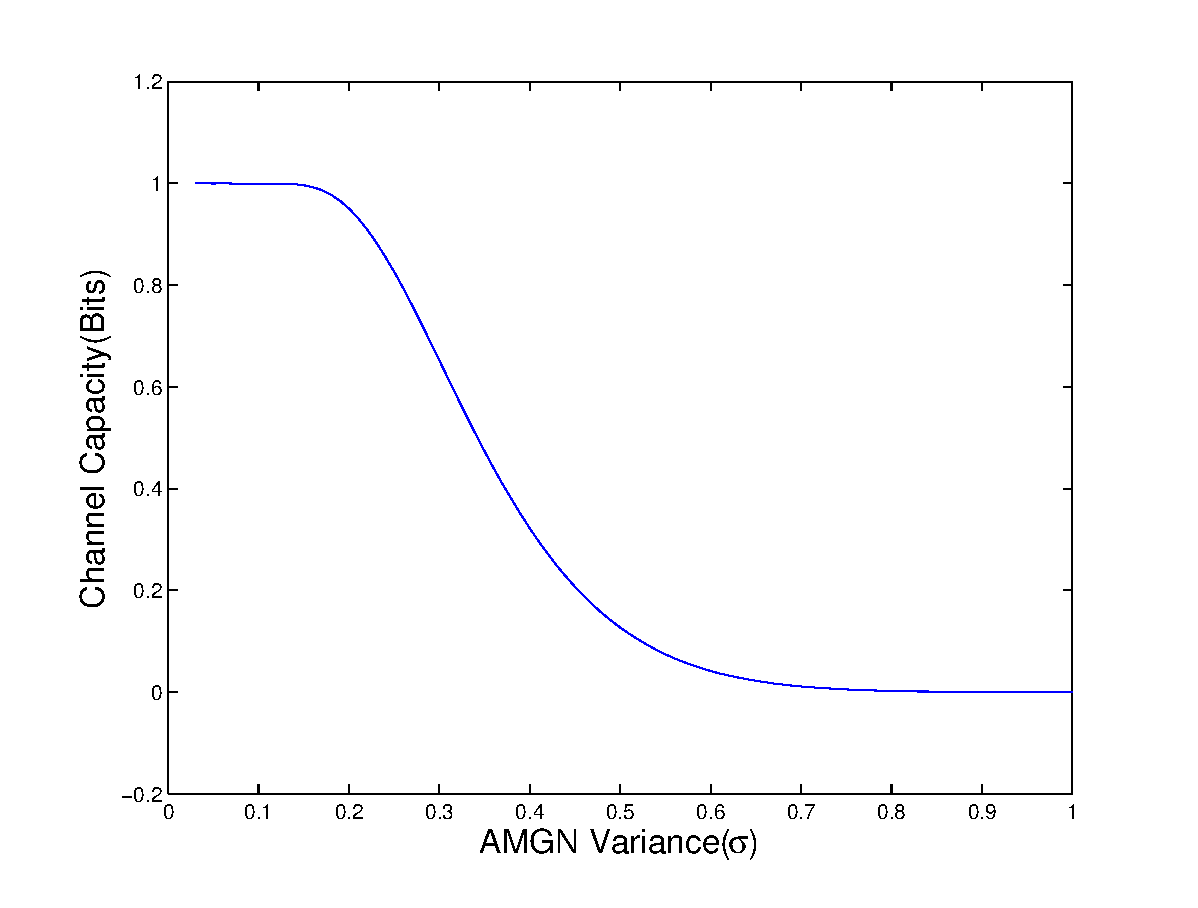
\includegraphics[width=0.9\textwidth]{./figures/SCLDPC_lattices/Cap_integer_coset_lattice.eps}
\caption{Channel capacity of the additive mod-2 Gaussian noise channel}
\label{Fig:AMGNCapacity}
\end{figure}

Plugging in the values of $n$ and the target error probability in \eqref{Eqn:ZLatticeProb} gives us $\sigma_{r+1}= 0.0804$. Now moving to the next level i.e., level $r$, $\sigma_{r}=2\sigma_{r+1}=0.1608$. The capacity of the effective AMGN channel observed in this level of the multi-stage decoding is $\tx{C}_{\tx{AMGN}}(\sigma^{2}_{r})=0.9923$, see Fig. \ref{Fig:AMGNCapacity}. For the details on computing the capacity of the AMGN channel see \cite{forney2000}.  Similarly proceeding, $\sigma_{r-1}=2\sigma_{r}=0.3217$, $\tx{C}_{\tx{AMGN}}(\sigma^{2}_{r-1})=0.5726$, $\sigma_{r-2}=2\sigma_{r-1}=0.6434$, $\tx{C}_{\tx{AMGN}}(\sigma^{2}_{r-2})=0.0242$. Observe that the capacity for level $r-2$ is almost zero which renders coding for this level unnecessary albeit at the cost of a very small increase in VNR (due to the rate loss) of $0.145$dB $(=20\log_{10}2^{0.0242})$. Hence $r=2$ i.e., two coded levels suffice. We use ($30,14,3$) CU-SC-LDPC ensemble with $L=32, w=4$ for the first two levels and $\Z_{4}^{n}$ lattice for the last level which results in nested SC-LDPC codes of rates $0.5333$ and $0.9$ ($0.49$ and $0.89$ including rate-loss due to boundary effects of coupling) matching closely the capacities of first two levels i.e. $0.5726$ and $0.99$.
\begin{table}
\centering
\caption{DE thresholds and Gap from Poltyrev limits (without rate loss from termination) for SC-LDPC lattice ensembles for various degree profiles.}
\begin{tabular}{c c c c c c}
\hline  \hline
$(d_{c},d_{v}^{1},d_{v}^{2})$ &(L,w)& $\sigma_{\text{max}}$ &$\text{VNR}^{*}$(dB) &$\text{VNR}_{\text{rate-loss}}$(dB)\\
\hline
(30,14,3) & (32,4) & 0.3184 & 1.14 & 1.347\\
(60, 27, 3)& (64, 9)  &  0.3203 & 0.57 & 0.951 \\
(60, 26, 3)& (72, 12) & 0.3200 &0.482 & 0.927\\
(60, 42, 3)& (72, 12) & 0.3975 & 0.203 &1.02\\
%(30,14,3) & (32,4) & 0.3184 &0.2184 &1.14dB&1.347dB\\
%(60, 27, 3)& (64, 9)  &  0.3203 & 0.1953 &0.57dB&0.951\\
%(60, 26, 3)& (72, 12) & 0.3200 & 0.1953 &0.482dB&0.927dB\\
%(60, 42, 3)& (72, 12) & 0.3975 & 0.1953 &0.203dB&---
%(60,42,3)&(72,12)&0.3975&0.1953&0.203dB\footnote{Target Bit Error Probability of $10^{-6}$}&---
\end{tabular}
\label{Table:Thresholds}
\end{table}

\subsubsection*{Simulation Results}
Due to symmetry in the lattice the all-zero lattice point is assumed to be transmitted. Instead of plotting the symbol error rate, we focus on determining the thresholds of the resulting lattice under BP decoding. We estimate the BP threshold from simulations by determining the maximum noise variance for which no codeword errors are observed, at each coded level, in simulation of 10 consecutive codewords each of length $2\times 10^{5}$. We calculate the maximum variance $\sigma_{\tx{max}}^{2}$ for which all the levels of the lattice can be decoded given by $\sigma_{\text{max}}=\min(\sigma_{1}^{\text{BP}},2\sigma_{2}^{\text{BP}},\sigma_{3})$, where $\sigma_{1}^{\text{BP}}$ and $\sigma_{2}^{\text{BP}}$ are the respective BP thresholds for the two SC-LDPC codes and $\sigma_{3}^{2}$ is the noise variance at which the uncoded level achieves the target error probability. The VNR threshold is then calculated for the given rates and $\sigma_{\text{max}}$. Thus obtained BP thresholds $\sigma_{1}^{\text{BP}}$, $\sigma_{2}^{\text{BP}}$ for the above codes are $0.3142$ and $0.2161$ respectively which results in a VNR of $1.14$dB ($1.46$dB with rate loss due to termination). The DE predicted values are $0.3184$ and $0.21836$. We observe that the BP thresholds are very close to DE thresholds. i.e., the parameters are large enough to assume that the BP thresholds can be approximated by DE thresholds. Therefore it is reasonable to calculate the VNR thresholds using the DE thresholds. For various SC-LDPC ensembles Table. \ref{Table:Thresholds} gives us the VNR thresholds i.e., the VNRs achievable for respective target error probabilities which are computed using the DE thresholds. Note that the Poltyrev limit is zero dB, thus making the VNR threshold and the gap from Poltyrev limit equivalent. The gap to the Poltyrev limit is primarily due to the fact that there is a mismatch between the capacity of the equivalent channel and the rates that are obtainable for the proposed CU-SC-LDPC ensemble.  

In the above design, if we target a error probability per dimension of $10^{-6}$  instead, that gives us $\sigma_{r+1}= 0.0999$, capacities for the subsequent levels $\tx{C}_{\tx{AMGN}}(\sigma^{2}_{r})=0.9507$, $\tx{C}_{\tx{AMGN}}(\sigma^{2}_{r-1})=0.3223$ and $\tx{C}_{\tx{AMGN}}(\sigma^{2}_{r-2})=0.0024$. Pair of nested codes from $(60,42,3)$ CU-SC-LDPC ensemble gives us rates $0.3$ and $0.95$ resulting in better matching of the rates (negligible rate loss). The resulting DE thresholds are within $0.203$dB from Poltyrev limit. This is reported in the last row in the table. [Couple of lines - Broadly justifying the VC-SC-LDPC construction] Observe that for these parameters we can use a $(60,4,3)$ VC-SC-LDPC ensemble with the same parameters of $(L=72,w=12)$ gives us codes of rates $0.25$ and $0.95$. Although this results in a slight VNR-loss due to the relatively poor mismatching of rates, in this case BP decoding is carried out on a $(3,4)$ Tanner graph instead of a $(42,60)$ which considerably reduces the complexity of decoding.

\section{Application - Interference Channel}
\subsection{Problem Statement}
We consider the 3 user Gaussian IC consisting of 3 transmitters, 3 receivers, and 3 independent messages originally considered in \cite{sridharan2008capacity}, where message $W_{j}$ originates at transmitter $j$ and is intended for receiver $j$, $\forall j\in \mc{J}\defeq\{1,2,3\}$. The output observed at the receiver $j$ is given by
\begin{align}\label{SymmInterfChannel}
    \mathbf{y}_{j}=\mathbf{x}_{j}+ \sum^{3}_{k=1,k\neq j}h_{jk}\mathbf{x}_{k}+\mathbf{z}_{j}, \hspace{10pt} \forall j\in \mc{J}
\end{align}
where $\mathbf{x}_{j}$ is the transmitted signal at $j^{\text{th}}$ transmitter, $h_{jk}$ are the channel parameters for the cross links, and $\mathbf{z}_{j}\sim\mc{N}(\mathbf{0},\sigma^{2}\cdot \mathbf{I})$ is the AWGN noise. If the channel parameters for all the cross links are equal we refer to such model as symmetric IC. The channel input signals are subjected to the power constraint
$\frac{1}{n}\sum_{i=1}^{n}E\left[\|\mathbf{x}_{j}\|^2\right]\leq P$.

For a $2$-user symmetric Gaussian interference channel (IC) it was shown in \cite{carleial1978interference} that, in the very strong interference regime, the capacity region for the IC is as if there is no interference at all. For this symmetric model, a simple extension of the very strong interference condition for the 2 user IC %\cite{carleial1978interference}
to the 3 user one is given by \cite{sridharan2008capacity}
\begin{align}
\beta^{2}\geq \frac{\left((1+P)^{2}-1\right)\left(1+P\right)}{2P}.
\label{Eqn:StrongInterfCondition1}
\end{align}

Sridharan \textit{et al.} in \cite{sridharan2008capacity} introduce the idea of lattice alignment where each user uses a lattice code and each receiver first decodes the total interference (aligned due to lattice structure) observed and then decodes the desired message. For this case, they
derived a tighter condition on $\beta$ in order for the interference to be decoded first. This is based on lattice coding, independent of the number of users, and is given by
\begin{align}
\beta^{2}(\sigma)\geq \beta^{*^{2}}(\sigma)\defeq\frac{(P+\sigma^{2})^{2}}{P\sigma^{2}}
\label{Eqn:StrongInterfCondition2}
\end{align}
If \eqref{Eqn:StrongInterfCondition2} is satisfied, each user can achieve a capacity \cite{sridharan2008capacity} of
$\frac{1}{2}\log(1+\frac{P}{\sigma^{2}})$. Equivalently, for a given rate $R$, maximum noise variance under which the rate can be achieved is given by
\begin{align}
\sigma^{2}_{\text{max}}=\frac{P}{2^{2R}-1}.
\label{Eqn:SigmaShannon}
\end{align}

\subsection{Applying the Proposed Lattices}
Encouraged by the Poltyrev-limit achieving property of the proposed lattice ensembles under BP decoding, we use SC-LDPC lattice codes for the symmetric Gaussian IC in the very strong interference region. Let $\Lmb_{SC}$ be the SC-LDPC lattice defined in \eqref{Eqn:ConstrD} with $r=2$.
% and a code from $(30,15,5)$ CU-SC-LDPC ensemble is used for the two levels.
We define the SC-LDPC lattice code $\mc{C}_{SCL}$ based on $\Lmb_{SC}$ using hypercube shaping:
\begin{align}
\mc{C}_{SCL}=\left\lbrace \mathbf{\lmb} \mod \Z_{4}^{n}: \mathbf{\lmb} \in \Lmb \right\rbrace
\end{align}
where $n$ is the dimension of $\Lmb_{SC}$. Let codeword $\mathbf{c}_{j}\in\mc{C}_{SCL}$ at transmitter $j$ be
\begin{align}
\mathbf{c}_{j}&= \sum_{i=1}^{k_{1}}\alpha_{ji}\mathbf{g}_i+2\sum_{i=1}^{k_{2}}\beta_{ji}\mathbf{g}_i \mod \Z_{4}^{n}\hspace{15pt} \alpha_{ji},\beta_{ji}\in \{0,1\}\\
\label{Eqn:SICCodeword}
&= \sum_{i=1}^{k_{1}}\alpha_{ji}\mathbf{g}_i+2\sum_{i=1}^{k_{2}}\beta_{ji}\mathbf{g}_i -4\mathbf{k}_{j}, \ \mbox{for some} \ \mathbf{k}_{j}\in\Z^{n}
\end{align}
where "$+$" denotes addition in $\R^{n}$. Each codeword $\mathbf{c}_{j}\in\mc{C}_{SCL}\subset\{0,1,2,3\}^{n}$ is modulated to $\mathbf{\tilde{x}}_{j}\defeq 1.5^{n}-\mathbf{c}_{j}$ such that $\mathbf{\tilde{x}}_{j}\in\mc{A}\defeq\{-1.5,-0.5,+0.5,+1.5\}^{n}$. At transmitter $j$, a dither vector $\mathbf{d}_{j}$ uniformly distributed among $\mc{B}\defeq [-2,2)$ is added to obtain the transmitted signal $\mathbf{x}_j$ given by
\begin{align}
\mathbf{x}_{j}=\mathbf{\tilde{x}}_{j}+\mathbf{d}_{j} \mod \Z_{4}^{n},
\label{Eqn:SICdither}
\end{align}
where the mod operation is over $\mc{B}$ instead of $[0,4)$. The dither vector achieves the purpose of randomizing the interference and helps in treating the undesired components of the received signal as additive uncorrelated noise. It can be seen that $\mathbf{x}_{j}$ is uniformly distributed over $\mc{B}$ and the average power of the transmitted signal at each transmitter is $1.33$.

\begin{figure*}[t]
\centering
\resizebox{0.8\textwidth}{!}{
%\begin{document}
\begin{tikzpicture}
\def\fsize{\small}
%3 Users
\draw[black] (0.4,0.2) rectangle (-0.4,-0.2); \node at (0,0) {\fsize Tx 1};
\draw[black] (0.4,-0.8) rectangle (-0.4,-1.2); \node at (0,-1) {\fsize Tx 2};
\draw[black] (0.4,-1.8) rectangle (-0.4,-2.2); \node at (0,-2) {\fsize Tx 3};

%Oblique lines to Plus block
\draw [->] (0.4,0) -- (1.75,0); \node [above] at (0.8,0) {1};
\draw [->] (0.4,-1) -- (1.75,0); \node [above] at (1,-0.65) {\large $\beta$};
\draw [->] (0.4,-2) -- (1.75,0); \node [above] at (1,-1.2) {\large $\beta$};


%From + end to Rx1 end
\draw[black] (2,0) circle (0.25); \node at (2,0) {+};
\draw [->] (2,-1) -- (2,-0.25);\node at (2.25,-0.9) {\large $\mathbf{z}_{1}$};

%Receiver 1 block
\draw[black] (2.7,-0.2) rectangle (3.5,0.2); \node at (3.1,0) {\fsize Rx 1};
\draw [->] (2.25,0) -- (2.7,0);\node[above] at (2.45,0) {\fsize $\mathbf{y}_{1}$};

%From Rx1 end to 1/beta multiplicator end
\draw[black] (4,0) circle (0.25); \node at (4,0) {$\times$};
\draw [->] (4,-0.75) -- (4,-0.25);\node at (4.15,-1) {\fsize $1/\beta$};
\draw [->] (3.5,0) -- (3.75,0);

\draw[black] (4.8,0.4) rectangle (6.2,-0.4) node[pos=0.5,align=center] {\footnotesize Subtract\\ $d_{2}\texttt{+}d_{3}$}; 
%\node[text width=1.2,align=left] at (5.05,0) {\fsize Subtract  \\ $d_{2}\texttt{+}d_{3}$};
\draw [->] (4.25,0) -- (4.8,0);

% Input to the Demod
\draw[black] (6.75,0.2) rectangle (8,-0.2) node[pos=0.5,align=center] {\small Demod};
\draw [->] (6.2,0) -- (6.75,0);

%Input to Decoder
\draw [->](8,0) -- (8.6,0) -- (8.6,-0.5);
\node[right] at (8.6,-0.2) {\fsize $\tilde{\mathbf{y}}_{1}$};
\draw[black] (8,-0.9) rectangle (9.2,-0.5) node[pos=0.5,align=center]  {\footnotesize Decoder}; 

%Overview dashed rectangle
\draw [->] (8.6,-0.9) -- (8.6,-1.3);  \node at (8.6,-1.5){\fsize $\mathbf{c_{2}}\texttt{+}\mathbf{c_{3}}$};
\draw [dashed] (2.6,-2.5) rectangle (9.4,1);\node [above] at (5,-2.5) {\fsize User 1};

 \end{tikzpicture}
%\end{document} 
}
\caption{System flow for the 3-user Symmetric Gaussian Interference channel at receiver 1.}
\label{Fig:SIC_decoder}
\end{figure*}

\subsection{Decoding}
Before looking at the general case let us consider the symmetric Gaussian IC i.e $h_{12}=h_{13}$. Without loss of generality let us consider receiver 1. The system flow from the perspective of receiver 1 is given in Fig.~\ref{Fig:SIC_decoder}. The input to the multistage decoder at receiver 1 is given by
\begin{align*}
\tilde{\mathbf{y}}_{1} &\defeq \frac{\mathbf{y}_{1}}{h_{12}}-\mathbf{d}_{2}-\mathbf{d}_{3}+1.5^{n}+1.5^{n}\\%\mod \Z_{4}^{n} \\
&=\mathbf{c}_{2}+\mathbf{c}_{3}+\frac{1}{h_{12}}\left(\mathbf{x}_{1}+\mathbf{z}_{1}\right).
\end{align*}
The key here is that $\mathbf{c}_{2},\mathbf{c}_{3}\in\mc{C}_{SCL}\subset\Lmb$ and hence $\mathbf{c}_{2}+\mathbf{c}_{3}\in \Lmb$.
\begin{align*}
\mathbf{c}_{2}+\mathbf{c}_{3}&=\sum_{i=1}^{k_{1}}\left(\alpha_{2i}+\alpha_{3i}\right)\mathbf{g}_i+2\sum_{i=1}^{k_{2}}\left(\beta_{2i}+\beta_{3i}\right)\mathbf{g}_i +4\mathbf{k}_{2}+4\mathbf{k}_{3}\\
&=\sum_{i=1}^{k_{1}}\left(\alpha_{2i}\oplus\alpha_{3i}\right)\mathbf{g}_i+2\sum_{i=1}^{k_{2}}\left(c_{1i}\oplus\beta_{2i}\oplus\beta_{3i}\right)\mathbf{g}_i +4\mathbf{k}_{23}
\end{align*}
where $c_{1i}=0.5\left(\alpha_{2i}+\alpha_{3i}-\alpha_{2i}\oplus\alpha_{3i}\right)$, $c_{2i}=0.5\left(c_{1i}+\beta_{2i}+\beta_{3i}-c_{1i}\oplus\beta_{2i}\oplus\beta_{3i}\right)$ are carryovers from first and second levels respectively and
 $\mathbf{k}_{23}=\mathbf{k}_{2}+\mathbf{k}_{3}+\sum_{1}^{k_{2}}c_{2i}\mathbf{g}_{i}\in\Z^{n}$. The key point is that $c_{1i}, c_{2i} \in \{0,1\}$. Using multi-stage decoder described in Section \ref{Sec:SCLDPC}, one can directly decode the lattice point $\mathbf{x}_{2}+\mathbf{x}_{3}$(interference), subtract it and decode the desired signal.

The decoding scheme above extends to the case when one channel gain is an integer multiple of the other. For example, let $h_{13}=Kh_{12}$
where $K=\sum_{0}^{l-1}a_{i}2^{i}\in \Z, a_{i}\in\{0,1\}$. In this case, input to the multi-stage decoder is
\begin{align*}
\tilde{\mathbf{y}}_{1} &\defeq \frac{\mathbf{y}_{1}}{h_{12}}-\mathbf{d}_{2}-K\mathbf{d}_{3}+1.5^{n}+K1.5^{n}\\
&=\mathbf{c}_{2}+K\mathbf{c}_{3}+\frac{1}{h_{12}}\left(\mathbf{x}_{1}+\mathbf{z}_{1}\right).
\end{align*}
where $\mathbf{c}_{2}+K\mathbf{c}_{3}$ is a lattice point and is given by
\begin{align*}
%\mathbf{c}_{2}+K\mathbf{c}_{3}=
\sum_{i=1}^{k_{1}}\left(\alpha_{2i}\oplus a_{0}\alpha_{3i}\right)\mathbf{g}_i+2\sum_{i=1}^{k_{2}}\left(c_{1i}\oplus\beta_{2i}\oplus a_{0}\beta_{3i}\oplus a_{1}\alpha_{3}\right)\mathbf{g}_i+4\mathbf{k}
\end{align*}
for some $\mathbf{k}\in\Z^{n}$.


\subsection{Simulation Results for Symmetric IC}
In this section we present simulation results for the symmetric Gaussian IC and compare them with the bounds given in \cite{sridharan2008capacity}. We choose a pair of nested codes from the $(30,18,3)$ CU-SC-LDPC ensemble with spatial-coupling parameters $(L,w)=(32,4)$. We fix $\sigma=\sigma_{\text{max}}$ (such that in absence of interference, desired signal can be decoded successfully) and we analyze the bit error probability in decoding the interference versus the channel gain $\beta$. We observe that within $0.396$dB of the very strong interference regime given by \eqref{Eqn:StrongInterfCondition2} we are able to decode the interference with a bit error probability of less than $10^{-6}$. Note that the main bottle neck in error performance in decoding the interference is the last i.e., the uncoded level whereas in decoding the desired signal (after the interference is decoded and subtracted), within $\sigma_{\text{max}}$, arbitrarily small error rates can be achieved since no uncoded level needs to be decoded.

%On a single user AWGN channel i.e, after the interference is subtracted, the DE threshold for this code for the given parameters is computed to be $\sigma_{\text{max}}=0.3351$ whereas asymptotically the maximum achievable variance is $\sigma_{\text{AMGN}}=0.3728$. The Shannon capacity from \eqref{Eqn:SigmaShannon} is given by $\sigma_{\text{Sh}}=0.4969$ which is equivalent to a gap of $2.5$dB.

In Fig.~\ref{Fig:ShapingLoss}, we plot the achievable rate as a function of $P/\sigma^2$ for the desired user for $r=4$. It can be seen that the achievable rate with the lattice code has a gap of roughly 1.53~dB from the corresponding Shannon limit at high rates. This is the shaping loss due to hypercube shaping.  The DE thresholds with the proposed SC-LDPC codes is also shown in the plot and it can be seen that the DE thresholds are very close to the achievable rates.
%
%We also observe that as the number of levels increase this gap converges to $1.53$dB which corresponds to the loss due to the sub-optimal hypercube shaping. For a 4-level binary lattice code with hypercube shaping corresponding gap between shannon capacity and the sum-capacity of 4 levels is plotted  in Fig. \ref{Fig:ShapingLoss}. One can also observe that the sum-capacity can be very closely achieved with a SC-LDPC lattice code of maximum check node degree 60.
%Thus we claim that with optimal shaping strategies the capacity of the $K$-user symmetric Gaussian IC \cite{sridharan2008capacity} in the very strong interference channel can be achieved.

\begin{figure}
\centering
\setlength\figureheight{0.7\textwidth}
\setlength\figurewidth{0.85\columnwidth}
\begin{tikzpicture}
\def\fsize{\normalsize}
\begin{axis}[
width=\figurewidth,
height=\figureheight,
scale only axis,
xmin=4,
xmax=30,
xlabel={$\text{P/}\sigma{}^{\text{2}}\text{dB}$},
ymin=0,
ymax=5,
legend style={at={(0,1)},anchor=north west,draw=black,fill=white,legend cell align=left}
]
\addplot [color=red,solid,line width=1.5pt]
table[row sep=crcr]{
1 0.587818317346194\\
3 0.791341177455778\\
5 1.0286866043034\\
7 1.29390718678102\\
9 1.58040221195651\\
11 1.88219718352143\\
13 2.19452948368152\\
15 2.51390383667526\\
17 2.83788995090244\\
19 3.16485622972095\\
21 3.49373172947796\\
23 3.8238235812452\\
25 4.1546876206064\\
27 4.48604077166048\\
29 4.81770328916082\\
31 5.14956130632863\\
33 5.48154279616551\\
35 5.81360224010802\\
};
\addlegendentry{Shannon Capacity};

\addplot [color=blue,solid,line width=2.0pt]
table[row sep=crcr]{
1 0.108452421861326\\
3 0.30023434461803\\
5 0.583744051972549\\
7 0.908016893863155\\
9 1.23986729393466\\
11 1.57212348172311\\
13 1.90441001540582\\
15 2.23669080702334\\
17 2.56895109146972\\
19 2.90120263165125\\
21 3.23173038940203\\
23 3.54445589072375\\
25 3.7941222586385\\
27 3.93912155348957\\
29 3.99069691963094\\
31 3.99949543839257\\
33 3.99999469407798\\
35 3.99999999597798\\
};
\addlegendentry{Sum Capacity of 4-level Construction-D Lattice Code};

\addplot [color=black,mark size=3.0pt,only marks,mark=square,mark options={solid}]
table[row sep=crcr]{
21.4693 3.15\\ % 18.91 3.1501 
22.3844 3.2667\\  %19.621 3.2668 . The commented out values are the snr values at which the shannon capacity is equal
23.1876 3.4167\\  %20.532 3.4166 	   to the DE of the optimal degree profiles of the 4 level SCLDPC lattice code.
15.4486951388326 2.2\\
16.3638449500461 2.3167\\
17.1669877129645 2.4667\\
};
\addlegendentry{DE thresholds for 4-level SC-LDPC Lattice Codes};

\addplot [color=black,mark size=2.9pt,only marks,mark=asterisk,mark options={solid}]
table[row sep=crcr]{
23.2798476914952 3.41666666666667\\
22.4669998480458 3.26666666666667\\
16.3950035382421 2.31666666666667\\
17.2078513816915 2.46666666666667\\
};
\addlegendentry{BP thresholds for 4-level SC-LDPC Lattice Codes};


\draw[<->] (axis cs:18.91,3.1501 ) -- (axis cs:21.469, 3.15);
\draw[->] (axis cs:19.6,3.12) to [out=285,in=175] (axis cs:22,2.6);
%\node[font=\scriptsize] at (axis cs:14,3.6){1.57dB};
\node[font=\fsize] at (axis cs:24,2.6){2.559dB};

	\end{axis}
\end{tikzpicture}%
\caption{Gap between the Shannon capacity and the sum-capacity of a 4-level Construction-D lattice code(hypercube shaping) under multi-stage decoding. The DE thresholds for various SC-LDPC lattice codes with a maximum check node degree of $60$ are also given.}	
\label{Fig:ShapingLoss}	
\end{figure}

%\section{Application - Bi-Directional Relay Channel}
%\subsection{Problem Statement}
%We consider the Bi-Directional Relay channel where two users try to communicate with each other with the help of a relay node acting as an intermediate. Objective is to design coding schemes at both the users and forwarding scheme at the relay such that at each user the message intended to be transmitted by the other user can be decoded, given the availability of the noise corrupted forwarded signal from the relay.
%The problem can be very simply described by these three equations: 
%\begin{align*}
%y_{R}=a x_{1}+b x_{2}+z \\
%y_{1}=x_{F}+z_{1} \\
%y_{2}=x_{F}+z_{2} 
%\end{align*}
% are received signals at Relay, and Users 1 and 2 respectively and $x_{F}$ is the signal forwarded by the relay and is a function of the  forwarding scheme we use. For simplicity let's assume that $a,b\in \Z$.
%
%\subsection{Proposed Scheme}
%We define a code (finite constellation) from the Poltyrev-good SC-LDPC lattice as follows:
%\begin{equation}
%\mc{C}\defeq \Lmb_{C}\cap \Z_{5}^{N}
%\end{equation}
%Rate of hence defined code will be $\log_{2}(2^{r_{1}+r_{2}}\frac{5}{4})=r_{1}+r_{2}+\log_{2}(\frac{5}{4})$ bits/dim. User $i$ picks a codeword $x_{i}\in\mc{C}$ uniformly and transmits. The received signal at relay is:
%\begin{align*}
%y_{R}=a x_{1}+b x_{2} +z
%\end{align*}
%The additive group structure of the lattice and the fact that $x_{1},x_{2}\in \Lmb_{C}$ gives us $a x_{1}+b x_{2}\in \Lmb_{C}$. Using the multi-stage decoding described previously we decode the lattice point $a x_{1} + b x_{2}\in \Lmb_{C}$. Note that in the decoder we need to do the euclidean decoder in the last stage too since not just the corresponding coset of $a x_{1}+b x_{2}$ suffices but we need the actual lattice point.

%For the forwarding part, we compute 
%\begin{align}
%x_{F}=a x_{1} +b x_{2} \mod 5\Z^{N}.
%\end{align}
%Note that since $5\Z^{N}\not \subset \Lmb_{C}$, $x_{F}\in \Lmb_{C}$ is not necessarily true. But for our application this won't be  a problem and we will see why subsequently.
%
%Let's consider User 1 and see how we can decode $x_{2}$ given $y_{1}=x_{F}+z_{1}$ .
% \begin{align*}
% y_{1}&=\left(a x_{1} +b x_{2} \right) \mod 5 +z_{1}\\
% &=\left[ a x_{1} \mod 5 +b x_{2} \mod 5 \right] \mod 5+z_{1}\\
% \end{align*}
%
%  \begin{align*}
%\left[ y_{1}-ax_{1}\right]\mod 5&=\left(\left(a x_{1} +b x_{2} \right) \mod 5 +z_{1}-ax_{1}\right)\mod 5\\
% &=\left[ a x_{1} \mod 5 +b x_{2} \mod 5 +z_{1} \mod 5 -a x_{1}\mod 5\right] \mod 5\\
%  &=\left[b x_{2} \mod 5 +z_{1} \mod 5 \right] \mod 5\\
% \end{align*}
% Assuming $b\not \equiv 0 \mod 5$, $\exists b^{-1}\in \Z_{5}$ such that $b^{-1}b\equiv 1\mod 5$.
%  \begin{align*}
%b^{-1}\left[ y_{1}-ax_{1}\right]\mod 5&=b^{-1}\left[b x_{2} \mod 5 +z_{1} \mod 5 \right] \mod 5\\
%&=\left[ x_{2} \mod 5 +b^{-1}z_{1} \mod 5 \right] \mod 5\\
%&=\left[ x_{2} +b^{-1}z_{1} \mod 5 \right] \mod 5\\
% \end{align*}
% The last step is because $x_{2}\mod 5=x_{2}\in \Lmb_{C}$ and hence we can decode $x_{2}\in \mc{C}$.
% \subsection{Performance : Analysis}
% This scheme, will be at a gap of atleast 1.53 dB from the AWGN channel capacity(for a given noise variance $\sigma^{2}$ for the uplink channel). If we can reduce this gap by using some vector quantzation scheme instead of the scalar quantization scheme( hypercube shaping) and at the same time avoid the zero divisor problem, that would be great.\\
% 
% Let $\Lmb_{S}$ be the shaping lattice generated using a convolutional code over $Z_{5}^{N}$ and then tessellating it over the entire space using $+5\Z^{N}$. \\
% Claim 1:We can guarantee that for all $x_{i},x_{j}\in \mc{C}$ and $x_{i}\neq x_{j}$, $x_{i} \mod \Lmb_{S}\neq x_{j}\mod \Lmb_{S}$. \\
% Claim 2: And also because of the tessellation, $x_{i} \mod \Lmb_{S}= x_{i}+5\mbf{k}\mod \Lmb_{S}$ for any $\mbf{k}\in \Z^{N}$.\\
%   With these two claims, if $x_{i}=\lmb_{i}\mod \Lmb_{S}$ for $i=1,2$,
%   \begin{align*}
%   y_{R}&=a(\lmb_{1}\mod \Lmb_{S})+b(\lmb_{2}\mod \Lmb_{S})+z\\
%   y_{R}\mod \Lmb_{S}&=(a\lambda_{1}+b\lmb_{2})\mod \Lmb_{S}+z\mod \Lmb_{S}\\
% 									&=\left[(a\lmb_{1}+b\lmb_{2})\mod 5\right]\mod \Lmb_{S}+z\mod \Lmb_{S}\\
%   \end{align*}
%   and there is no guarantee that $(a\lmb_{1}+b\lmb_{2})\mod 5\in \Lmb_{C}\cap \Z_{5}^{N}$ and hence in decoding $a x_{1}+bx_{2}\mod \Lmb_{S}$ we loose the error performance protection afforded by the SC LDPC codes in the Coded Lattice $\Lmb_{C}.$
%   
%   Hence as of now, the shaping loss of 1.53dB looks unavoidable tif we want to avoid the zero divisor problem. %SCLDPC

--------------------Compressed Sensing--------------------------------
\chapter{COMPRESSED SENSING}
\label{chap:cs}
%In \cite{li2015subisit,li2015subdraft}, two schemes have been proposed to recover the support of a $K$-sparse $N$-dimensional signal from noisy linear measurements. Both schemes use left-regular sparse-graph code based sensing matrices and a simple peeling-based decoding algorithm. Both the schemes require $O(K \log N)$ measurements and the first scheme require $O(N \log N)$ computations whereas the second scheme requires $O(K \log N)$ computations (sub-linear time complexity when $K$ is sub-linear in $N)$. We show that by replacing the left-regular ensemble with left and right regular ensemble, we can reduce the number of measurements required of these schemes to the optimal order of $O\left(K \log \frac{N}{K} \right)$ with decoding complexities of $O(K \log \frac{N}{K})$ and $O(N \log \frac{N}{K})$, respectively.

\section{Introduction}
The classical problem of compressed sensing involves estimating a signal $\mbf{x}$, which is sparse in some basis, from a noisy measurement signal $\mbf{y}$ of smaller dimension compared to $\mbf{x}$. Formally, let
\begin{align*}
\mbf{y=Ax+w},
\end{align*}
where $\mbf{x}$ is an $N$-dimensional vector, $\mbf{A}$ is a known $M \times N$ matrix commonly referred to as \emph{measurement matrix} and $\mbf{w}$ is additive noise. The unknown signal $\mbf{x}$ is known to be sparse in some basis and we denote the sparsity of $\mbf{x}$ by $K$. If there is no noise, then we refer to it as the noiseless setting. It is known that if $K \ll N$ we can recover the unknown signal in significantly fewer number of measurements compared to $N$.  Particularly in this chapter we focus on recovering the support of $\mbf{x}$ defined as supp$(\mbf{x}):=\{i:x_i\neq 0, i\in[N]\}$ where $\mbf{x}=[x_1,\ldots , x_i \ldots ,x_N]^{T}$ and $[N]\coleq\{1,2,\ldots ,N\}$. For a given scheme, given the reconstruction vector $\widehat{\mbf{x}}$, we consider the probability of failure of support recovery which can be defined as
\begin{align*}
\mbb{P}_{F}\coleq\Pr(\text{supp}(\widehat{\mbf{x}})\neq \text{supp}(\mbf{x})).
\end{align*}
 For the support recovery problem, under noisy settings, Wainwright \cite{wainwright2009information} showed information theoretically that $O\left(K\log(\frac{N}{K})\right)$ number of measurements is necessary and sufficient for asymptotically reliable recovery.

In \cite{li2015subisit} (and in the expanded version in \cite{li2015subdraft}), Li, Pawar and Ramchandran have considered the compressed sensing problem of recovering the support of a $K$-sparse, $N$-dimensional signal from $M$ linear and noisy measurements. Based on sparse-graph codes with a \emph{left-regular} degree profile and a peeling decoder, they have proposed an elegant design of the measurement matrix and a recovery algorithm. They have proposed two designs - the first design requires $M = \mc{O}(K \log N)$ measurements and a near-linear $\mc{O}(N \log N)$ decoding complexity, whereas the second design requires $M = \mc{O}(K \log N)$ measurements with a sub-linear $\mc{O}(K \log N)$ decoding complexity.
%This combination is shown to provide order-wise optimal measurement complexity (number of measurements) and computational complexity.

In this chapter\cite{vem2016sub}, we show that the bounds on the measurement complexity reported in \cite{li2015subisit,li2015subdraft} can be improved by considering \emph{left-and- right-regular} sparse-graph based sensing matrices. We show that only $\mc{O}\left(K \log \frac{N}{K} \right)$ measurements are required when $K = \mc{O}(N^\delta)$, for any $0 \leq \delta < 1$, to recover the support with the optimal sub-linear time decoding complexity.  This matches the information-theoretic lower bound on the number of measurement required for asymptotically-reliable recovery \cite{wainwright2009information}. Also, through simulations we demonstrate that the proposed scheme has superior performance compared to \cite{li2015subdraft}.
%For sub-linear time decoding complexity, we show that only $O\left(K \log^{1.3} \frac{N}{K} \right)$ are required. Finally, we also provide sharper version of the results in \cite{li2015subdraft}. 

The literature on compressed sensing is vast and it is difficult to provide a comparison with several of the existing results in the literature due to different error performance metrics being used for different versions of the problem. Nevertheless, it should be pointed out that the use of left and right regular bipartite graphs as choice for sensing matrix has been proposed in \cite{jafarpour2009efficient} and the measurement complexity has been shown to be only $\mc{O}\left(K \log \frac{N}{K} \right)$. However, the decoding complexity is near-linear $\mc{O}(N\log \frac{N}{K})$. We achieve a similar measurement complexity but with optimal computational complexity of $\mc{O}(K\log \frac{N}{K})$. Also unlike in \cite{jafarpour2009efficient} the sensing matrix in this chapter is constructed based on a tensor-product construction and the decoding algorithm is based on identifying singletons and peeling them off.

% sensing scheme and the decoding algorithm in this chapter are different from those in \cite{jafarpour2009efficient} and are based directly on those in \cite{li2015subisit,li2015subdraft}. 
 
For the information-theoretic lower bound in \cite{wainwright2009information} to hold, the non-zero elements in $\mbf{x}$ should have a sufficiently large minimum absolute value. In view of this condition, similar to \cite{li2015subisit,li2015subdraft}, we assume that all the non-zero elements of $\mbf{x}$ belong to the set $\{Ae^{i\theta}:A\in\mc{A},\theta\in\Theta\}$ where $\mc{A}\coleq \{A_{\text{min}}+\rho l\}^{L_1}_{l=0},\Theta\coleq\{2\pi l/L_2\}_{l=0}^{L_2}$ for finite but arbitrarily large integers $L_1$ and $L_2$.

%we set a minimum absolute value for the non-zero elements and further assume that they are from a discrete set. More precisely for the noisy setting
\section{Prior work}
\label{Sec:Review}
In this section, we review the construction of the measurement matrix $\mbf{A}$ proposed by Li, Pawar and Ramchandran in \cite{li2015subisit} and \cite{li2015subdraft}, and also summarize their key results. To keep the discussion simple, we omit certain details and refer readers to the original work \cite{li2015subisit} (and the expanded version  \cite{li2015subdraft}).

%The main idea is to use the sparse-graph based construction to decompose the problem of $K$-sparse support recovery into 1-sparse problems and then use a simple peeling based decoder \cite{richardson2008modern} to recover the support.
The measurement matrix is constructed using a combination of a sparse-graph code defined by the $R \times N$ coding matrix ${\bf H=[h_1, h_2, \cdots ,h_{N}]} \in {\{0,1 \}}^{R \times N}$  and a $P \times N$ bin-detection matrix $\bf S=[s_1, s_2, \cdots ,s_N]$. The coding matrix $\bf H$ defines a bipartite graph $\mathcal{G}$ with $N$ left (variable) nodes, representing the $N$-length signal $\bf x$, and $R$ right (check) nodes representing the measurements  $\bf y=[y_1, y_2, \cdots, y_R]$. Let $q_i, i\in [R]$, be the number of non-zero variable nodes connected to $i^{\text{th}}$ check node. Assume an ``oracle" that solves the 1-sparse problem by examining each check node observations and classifies it as a zero-ton($q_i=0$), singleton($q_i=1$) or a multi-ton($q_i>1$), and also identifies the position $\hat{k}$ and value $\widehat{x}_{\hat{k}}$ of the participating variable node if it is a single-ton. Once a singleton is identified the corresponding variable node's contribution is peeled off from other participating check nodes and this process creates new single-tons. The decoding process continues until there are no more singletons. The decoding is successful if all the $K$ non-zero elements of $\bf x$ are recovered at the end of decoding.

The  $RP \times N $ measurement matrix $\bf A$ with $M = RP$ measurements is constructed by taking the row tensor product $ \boxtimes$ of $\bf H$ and $\bf S$ given by
\[
 \bf A = H \ { \boxtimes} \ S := [h_1 \otimes s_1, h_2 { \otimes} s_2, \cdots , h_N { \otimes} s_N]
 \]

where $\otimes$ is the standard Kronecker product.

%They explore both $\textit{l}$-left regular and irregular ensembles for the $\bf H$ matrix construction and provide analysis for the left regular case.
For the noisy setting, they have proposed three designs for $\bf S$ which essentially performs the role of the oracle in identifying a single-ton at each check node. These designs are \emph{RandomNoisy} with near-linear decoding complexity, \emph{BinaryNoisy} and \emph{FourierNoisy} each with sub-linear decoding complexity.
%The only difference in these designs is the $\bf S$ matrix construction and hence the 1-sparse(bin detection) problem solving methodology.
The bin-detection matrix $\bf S$ for the three settings are as follows:
\begin{itemize}
\item \emph{RandomNoisy:}  Ensemble of $P \times N$ matrices $S = [S_{i,j}]_{P \times N}$ where $S_{i,j}$ $’$s are i.i.d. sub-gaussian entries with zero mean and unit variance.

\item  \emph{FourierNoisy}:  $\bf S = [S_0 S_1 \cdots S_{P-1}]^{T}$, where $\bf S_p$ consists of $Q=O(\log^{1/3}N)$ consecutive $2^p$-dyadically spaced rows from the $N \times N$ DFT matrix.

\item \emph{BinaryNoisy:}  $\mbf{S} = f(\mbf{C})$ where $\mbf{C}_{P \times N}$ is a binary codebook(or subset of a codebook) of a linear code with block length $P$, $f:\{0,1\}^q\rightarrow \mc{M}$ is a modulation scheme that maps $C_{P \times N}$ to $S_{\frac{P}{q}\times N}$. For e.g., for QAM $q=2$ and $\mc{M}=\{\pm 1 \pm i\}$.
\end{itemize}

The following theorems from \cite{li2015subdraft} summarize their key results.

%\begin{theorem}[\cite{li2015subdraft} Noiseless recovery]\label{thm:li1}
%In the absence of noise, given any $K$-sparse signal $\mbf{x}$ with $x_k \in \mathcal{X}$ for $k \in \text{supp} \mbf{(x)}$, their noiseless recovery schemes achieve a vanishing failure probability $\mathbb{P}_F(O\left(\frac{1}{K})\right) \rightarrow 0$ asymptotically in $K$ and $N$ with
%\begin{center}\small
%\begin{tabular}{|c|c|c|}
%  \hline
%   &  $M$ &  $T$ \\
%  \hline
%  Fourier noiseless & $2(1+\epsilon)K$ & $O(K)$ \\
%  \hline
%  Binary noiseless & $(1+\epsilon)K(\log_2 N+1)$ & $O(K \log N)$ \\
%  \hline
%\end{tabular}
%\end{center}
%where $M$ and $T$ are measurement cost and computational complexity respectively.
%\end{theorem}
%\vspace{2ex}


\begin{theorem}[\cite{li2015subdraft} Sub-linear Time Noisy Recovery]\label{thm:li2} In the presence of i.i.d. Gaussian noise with zero mean and
variance $\sigma^2$, given any $K$-sparse signal $\mbf{x}$ with $x_k \in \mathcal{X}$ for $k \in \text{supp}(\mbf{x})$, our noiseless recovery schemes achieve a vanishing failure probability $\mathbb{P}_F \rightarrow 0$ asymptotically in $K$ and $N$ with
\begin{center}\small
\begin{tabular}{|c|c|c|}
  \hline
   & $M$ &  $T$ \\
  \hline
  Fourier noisy & $O(K \log^{1.3}N)$ & $O(K \log^{1.3}N)$ \\
  \hline
  Binary noisy & $O(K \log N)$ & $O(K \log N)$ \\
  \hline
\end{tabular}
\end{center}
where $M$ and $T$ are measurement cost and computational complexity respectively.
\end{theorem}
\vspace{2ex}

\begin{theorem}[\cite{li2015subdraft} Near-linear Time Noisy Recovery]\label{thm:li3} In the presence of i.i.d. Gaussian noise with zero mean and
variance $\sigma^2$, given any $K$-sparse signal $\mbf{x}$ with $x_k \in \mathcal{X}$ for $k \in \text{supp}(\mbf{x})$, the RandomNoisy scheme achieves a vanishing failure probability $\mathbb{P}_F \rightarrow 0$ asymptotically in $K$ and $N$ with a measurement complexity of $M = O(K \log N)$ and computational complexity of $T = O(N \log N)$.
\end{theorem}

\section{Proposed scheme}
%\subsection{Main Idea}
The main difference between \cite{li2015subdraft} and our approach is that we replace the left $l$-regular ensemble of graphs corresponding to the coding matrix $\mbf{H}$ described in Sec \ref{Sec:Review} by left {\em and} right $\left(l, r\right)$-regular ensemble of graphs.

\begin{definition}[Left and right regular graph ensemble]\label{def:leftandrighreg}
Let $\mathcal{G}^N_{\rm reg,reg}\left(R,l, \frac{lN}{R} \right)$ denote the ensemble of left and right regular bipartite graphs with $N$ variable nodes and $R$ check nodes, where each variable node $k \in [N]$ is connected to $l$ check nodes and each check node $j \in [R]$ is connected to $\frac{lN}{R}$ left nodes.
\end{definition}
In the design considerations of bin detection matrix, we now have only $r=\frac{lN}{\eta K}=O\left(\frac{N}{K}\right)$ variable nodes connected to each check node and thus we require only a bin detection matrix $\mbf{S}$ with $O(\frac{N}{K})$ columns. For the bin detection matrix designs in Sec. \ref{Sec:Review} we know from \cite{li2015subdraft} that to differentiate between a zero-ton, singleton and a multi-ton successfully with probability approaching $1$ asymptotically in $\frac{N}{K}$ we only require $\log(\frac{N}{K})$ rows in $\mbf{S}$. We choose the bin detection matrix to be similar to the \emph{RandomNoisy, FourierNoisy, BinaryNoisy} designs but with dimensions $P'\times r$ where $P'=O\left(\log(\frac{N}{K})\right)$.

We know from the modern coding theory that to peel off $K$ unknown variable nodes successfully from the bipartite graph we need $\eta K$ number of check nodes for some $\eta>1$. So we choose the number of check nodes $R = \eta K$. A matrix $\mathbf{H}$ is chosen at random from this ensemble $\mathcal{G}^N_{\rm reg,reg}\left(\eta K,l, \frac{lN}{\eta K} \right)$ and used as the coding matrix.

The measurement matrix $\bf A$ for the proposed construction with $\bf H_{R \times N} = [h_1, h_2, \cdots, h_N]^{T}$ and $\bf S_{P' \times r}= [s_1, s_2, \cdots ,s_r]$ is given by $ {\bf A}_{RP' \times N} = {\bf H \boxplus S }$,
 where $ \boxplus$ is the new tensoring operation, which is slightly different from the row-tensor operation used in Sec \ref{Sec:Review} and is defined as
  \[ {\bf A}_{RP' \times N} = {\bf H \boxplus S } = \begin{bmatrix} \bf
 h_1 \boxtimes S_1 \\ \bf
 h_2 \boxtimes S_2 \\ \bf
 \vdots\\ \bf
 h_R \boxtimes S_R  \bf
\end{bmatrix}  \]

 where, \\
 $\bf S_i= [0, \cdots, s_1 , 0, \cdots, s_2, \cdots, 0, s_r, \cdots, 0],$ $(i\in[R])$, where $\bf 0$ is an all-zero column vector of length $P'$ placed in positions $j$ where $h_{ij}=0$ and the column vectors $\bf s_k$, $k\in[r]$ are placed sequentially in the positions $j$ where $h_{ij}=1$.
We illustrate the new tensoring operation $\boxplus$ via Example~\ref{exmp:tensorA}.

% New tensoring operation example.
\begin{example}\label{exmp:tensorA}
Let \[H = \begin{bmatrix}
1 & 0 & 0 & 1 & 0 & 1    \\
0 & 1 & 1 & 0 & 1 & 0 \\
1 & 1 & 0 & 1 & 0 & 0 \\
0 & 0 & 1 & 0 & 1 & 1
\end{bmatrix} \] denote an adjacency matrix from the ensemble  $\mathcal{G}^6_{\rm reg,reg}\left(4,2,3 \right)$. We choose $P'= \lceil \log_2 r \rceil = 2$ and let $S_{P' \times r}$ be defined as  
\[ S = \begin{bmatrix}
+1 & -1 & -1\\
-1 & +1 & -1
\end{bmatrix} \]
Then, the measurement matrix $\bf A$ with $M = P'R = 8$ measurements is given by 
\[ A = H \boxplus S \ = \begin{bmatrix}
+1 & \ \ 0 & \ \ 0 & -1 & \ \ 0 & -1\\
-1 & \ \ 0 & \ \ 0 & +1 & \ \ 0 & -1\\
\ \ 0 & +1 & -1 & \ \ 0 & -1 & \ \ 0\\
\ \ 0 & -1 & +1 & \ \ 0 & -1 & \ \ 0\\
+1 & -1 & \ \ 0 & -1 & \ \ 0 &\ \ 0\\
-1 & +1 & \ \ 0 & -1 & \ \ 0 &\ \ 0\\
\ \ 0 & \ \ 0 & +1 & \ \ 0 & -1 & -1\\
\ \ 0 & \ \ 0 & -1 & \ \ 0 & +1 & -1
\end{bmatrix}
 \]

 \end{example}

\section{Improved bounds}
%\subsubsection*{Main Results}
With our proposed construction of the measurement matrix, Theorem~\ref{thm:li2} and Theorem~\ref{thm:li3} can be sharpened to the following new theorems.
\begin{theorem}[Sub-linear Time Noisy Recovery]\label{Thm:ourSubLinearNoisy}  In the presence of i.i.d. Gaussian noise with zero mean and
variance $\sigma^2$, given any $K$-sparse signal $\mbf{x}$ with $x_k \in \mathcal{X}$ for $k \in \text{supp} (\mbf{x})$, our noisy recovery schemes achieve a vanishing failure probability $\mathbb{P}_F \rightarrow 0$ asymptotically in $K$ and $N$ with
\begin{center}
\begin{tabular}{|c|c|c|}
  \hline
   & $M$ &  $T$ \\
  \hline
  Fourier noisy & $O\left(K \log^{1.3} \frac{N}{K} \right)$ & $O\left(K \log^{1.3} \frac{N}{K} \right)$ \\
  \hline
  Binary noisy & $O\left(K \log \frac{N}{K} \right)$  & $O\left(K \log \frac{N}{K} \right)$ \\
  \hline
\end{tabular}
\end{center}
\end{theorem}

\begin{theorem} [Near-linear Time Noisy Recovery]\label{Thm:ourNearLinearNoisy} In the presence of i.i.d. Gaussian noise with zero mean and
variance $\sigma^2$, given any $K$-sparse signal $\mbf{x}$ with $x_k \in \mathcal{X}$ for $k \in \text{supp} (\mbf{x})$, the RandomNoisy scheme achieves a vanishing failure probability $\mathbb{P}_F \rightarrow 0$ asymptotically in $K$ and $N$ with a measurement complexity of $M = O \left( K \log \frac{N}{K} \right)$ and computational complexity of $T = O \left( N \log \frac{N}{K} \right)$.
\end{theorem}

\begin{proof}
The bin detection matrix and the decoding methods employed to identify a singleton are identical to that of \cite{li2015subdraft} except that $P=O(\log N)$ is replaced by $P'=O\left(\log(\frac{N}{K})\right)$. Hence the probability of error for the bin detection algorithm can be analyzed exactly as in \cite{li2015subdraft} with $P'$ replaced by $P$ and thus can be shown to be exponentially decaying in $P'$. For this particular choice of $P'$ the probability of error for the bin detection part vanishes asymptotically in $\frac{N}{K}$. Therefore for $K$ sub-linear in $N$ all it remains to be shown is that the $\mathcal{G}^N_{\rm reg,reg}\left(R,l, \frac{lN}{R} \right)$ ensemble with peeling process fails with a vanishing error probability $\mbb{P}_F$ asymptotically in $K$ and $N$. For choice of $l\geq 3$,  Theorem~\ref{Thm:PeelingOptimal} gives us this required result and that completes the proof.
\end{proof}

%By using the left and right regular ensemble we are able to achieve the order optimal bounds for measurement cost. However, there will be a penalty to pay in terms of the minimum SNR required and this is discussed next.
%\subsection{Minimum SNR required}
%We will take the \emph{RandomNoisy} case as an example and let us consider the case when $K = O(N^\delta)$ for some $0 \leq \delta < 1$.  In the derivation of the probability of error in \cite{li2015subdraft} in Proposition 3 and Proposition 4 in Appendix D, it can be seen that the probability of error includes terms of the form
%\[
%e^{-\frac{P}{4} \frac{\gamma^2}{1+4\gamma}} + 2 e^{-c_6 P \left(1-\frac{\gamma \sigma^2}{A^2_{\rm min}} \right)}.
%\]
%%Right after Proposition~5, i
%It is mentioned that by choosing $P = O(\log N)$, the probability of error can be made to decay as $O\left(\frac{1}{N^3} \right) <  O\left(\frac{1}{K^3} \right)$. First, it should be noted that when $P = O(\log N)$, in order for the probability of error to decay as $O\left(\frac{1}{K^3} \right)$, the following two conditions must be satisfied on $\gamma$
%\[
%\frac{\gamma^2}{4(1+4\gamma)} > 2 \delta, \ \ {\rm and} \ c_6 \left(1 - \frac{\gamma \sigma^2}{A_{\rm min}^2} \right) > 2 \delta
%\]
%
%Hence, for the overall probability of error to decay as $O(1/K^3)$, $A_{\rm min}^2/\sigma^2$ should be large enough such that $0 < 2 \delta < \gamma < A_{\rm min}^2/\sigma^2$. Hence, the theorems appear to be valid only for $A_{\rm min}^2/\sigma^2 > SNR_{\rm Th}$.
%
%\subsection{SNR versus Measurements}
%It should be noted that if the objective is to get the probability of error to decay only as $O(1/K^3)$, it is not required for the probability of error to decay as $O(1/N^3)$ and hence, we could directly choose $P = O(\log N/K) =O\left((1-\delta) N\right)$
% or in fact, $P = O(\log N^\beta)$ for any $\beta$ and that there will be a corresponding $SNR_{\rm Th}$. Indeed, this appears to reasonable since the assumption that the non-zero values of the signals are from a finite set and hence, when the $\sigma^2 \rightarrow 0$, the number of samples required should smoothly go to $O(K)$. Hence, it appears that the order of measurements required should be a function of SNR.
%
%%Based on this, indeed, it appears that when using RandomNoisy measurement matrix, it is not even required to switch to the $\mathcal{G}_{\rm reg-reg}$ ensemble and we could have simply chosen $P = O(N^\beta)$. However, if we want to choose the Random DFT ensembele (see Page 22 \cite{li2015subdraft}), then we have to switch to the $\mathcal{G}_{\rm reg-reg}$. It appears convenient to switch to this ensemble for all results

\section{Proofs}
In this section we consider a $\mathcal{G}^{N}_{\rm reg,reg}(R,l,\frac{lN}{R})$ ensemble and show that this ensemble with the oracle based peeling decoder fails to recover all the variable nodes with a probability of at most $O\left(\frac{1}{K}\right)$. Although it appears this can be achieved directly by using a capacity achieving spatially-coupled LDPC ensemble and use the existing results, there are two main obstacles to this:
\begin{itemize}
\item  In traditional LDPC codes and peeling decoder over binary erasure channel, the input to the decoder is the channel output corresponding to $N$ variable (bit) nodes and the check nodes on the right are mere parity checks whose sum modulo 2 is zero. Whereas in our problem the values corresponding to the $N$ variable nodes on the left need to be evaluated by the decoder given the values corresponding to the $R$ check nodes (the real sum of the variable nodes connected) are non-zero  and form input to the decoder.
\item  In traditional LDPC case a constant fraction $\epsilon$ of these $N$ variable nodes are erased by the channel and usually the emphasis is on analyzing the performance of peeling decoder asymptotically in $N$ or $R$ when rate=$1-\frac{R}{N}$ is fixed. But in our case the fraction of the nodes erased $=1-\frac{K}{N}$, where $K$, sub-linear in $N$, is usually of the form $K=N^{\delta}$, tend to one and the rate of the code$=1-\frac{R}{N}=1-\frac{\eta N^{\delta}}{N}$ tend to one asymptotically in $N$.
\end{itemize}
\vspace{1ex}

Consider a left and right regular LDPC code $\mathcal{G}_{\text{LDPC}}(N,l,r)$ where $N$ is the number of variable nodes on the left and $l,r$ are the regular left and right degrees respectively. Let $\text{P}_{\text{BEC}}^{(i)}(\mathbf{y})$ be the degree distribution of the number of check nodes after iteration $i$ of peeling decoder given $\mathbf{y}$ is the channel output. And similarly $\mathcal{G}^{N}_{\text{reg,reg}}(R,l,\frac{lN}{R})$ be the graph corresponding to the parity check matrix in the support recovery problem and $\text{P}_{\text{SR}}^{(i)}(\mathbf{z})$ be the degree distribution of the check nodes on the right after iteration $i$ of the oracle-based peeling decoder, given $\mathbf{z}$ is the support recovery equivalent of syndrome corresponding to $\mathbf{x}$ i.e., $\mbf{z}=\mbf{H}\mbf{x}$ where the operations are over the real field.
% Note that $\mbf{y}$ is a vector of dimension $N$ whereas $\mbf{z}$ is of dimension $\frac{Nl}{r}$.\\

Note that in the peeling decoder, we peel off one degree-1 check node and the variable node connected to it from the graph in each iteration. In the LDPC-BEC problem we remove all the variable nodes that are not erased by the channel and the resulting graph is input to the decoder. Similarly in the case of support recovery problem we consider the  oracle based peeling decoder in \cite{li2015subdraft} and we analyze the \textit{pruned}-graph where we remove all the zero variable nodes from the original graph and input to the decoder.

\begin{lemma}[Equivalence to LDPC-BEC]
\label{Lemma:Equiv_LDPC_BEC}
Whenever $\mbf{y}$ and $\mbf{z}$ satisfy
\begin{align*}
\mbf{z=Hx} \text{ such that  } S:=|\text{supp}(\mbf{x})|=|\{i:y_i=\mathcal{E}\}|  \qquad
\end{align*}
where $\mathcal{E}$ denotes erasure, then $\text{P}_{\text{BEC}}^{(i)}(\mbf{y})=\text{P}_{\text{SR}}^{(i)}(\mbf{z}) \quad \forall i$.
\end{lemma}
\begin{proof}
Define $S^c=[1:N]\backslash S$. In the case of LDPC codes on BEC we peel off all non-erased variable nodes corresponding to $S^c$  and input the resulting graph to the peeling decoder. Similarly in the case of bipartite graph in support recovery problem we peel off all the zero nodes corresponding to $S^c$ and we input the resulting graph to oracle based peeling decoder. From this point onward the peeling decoders are identical and thus we have our result.
\end{proof}
\vspace{1ex}
%The above lemma gives us the equivalence of peeling decoder of LDPC codes on BEC and oracle based peeling decoder of compressed sensing problem.
Thus by considering a BEC of erasure probability $\epsilon=\frac{K}{N}$ we can equivalently consider peeling decoder of LDPC codes on BEC channel and use various existing results.
\begin{lemma}
\label{lem:RightDegEvolution}
The evolution of the left and right degree distribution as the peeling decoder progresses can be given by
\begin{align*}
\tilde{L}_l(y)&= y^kl,\\
\tilde{R}_{1}(y)&=r\epsilon y^{l-1}[y-1+ (1-\epsilon y^{l-1})^{r-1}]\\
\tilde{R}_{i}(y)&=\binom{r}{i}(\epsilon y^{l-1})^i (1-\epsilon y^{l-1})^{r-1}, \quad i\geq 2
%\tilde{R}_{0}(y)&=1-\sum_{j\geq 1}\tilde{R}_{j}(y),\\
\end{align*}
where $\epsilon=\frac{K}{N}$ and $r=\frac{lN}{\eta K}$. Note that the curve corresponding to $\tilde{L}_i(y)(\tilde{R}_{i}(y))$ for $y\in[0,1]$ gives the expected number of degree $i$ variable nodes (check nodes) normalized with respect to $K$ ($\eta K)$.
\end{lemma}
\begin{proof}
As we showed in Lemma.~\ref{Lemma:Equiv_LDPC_BEC} the peeling decoder for an LDPC on BEC channel and oracle based peeling decoder for CS are identical upto the residual degree distributions at each iteration. Hence we can use the result for LDPC codes \cite[Theorem~3.107]{richardson2008modern} with equivalent channel erasure probability $\epsilon=\frac{K}{N}$.
\end{proof}

\begin{definition}[BP Threshold]
We define the BP threshold, $\eta^{\text{BP}}$ to be the minimum value of $\eta$ for which there is no non-zero solution for the equation:
\begin{align*}
y&=\lim_{\frac{N}{K}\rightarrow\infty}1-\left(1-\frac{Ky^{l-1}}{N}\right)^{\frac{lN}{\eta K}}\\
  &=1-e^{\frac{-ly^{l-1}}{\eta}}
\end{align*}
in the range $y\in [0,1]$.
\end{definition}

\begin{lemma}\cite[Theorem~3.107]{richardson2008modern}
\label{lem:PeelSmallGraph}
If $\eta>\eta^{BP}$ then with probability at least $1-O\left(K^{1/6}e^{-\frac{\sqrt{Kl}}{(lr)^3}}\right)$ the peeling decoder of a specific instance progresses until the number of residual variable nodes in the graph has reached size $\gamma K$ where $\gamma$ is an arbitrary positive constant.
\end{lemma}

\begin{definition}[Expander Graphs]
\label{Def:ExpanderGraph}
A bipartite graph with K left nodes and regular left degree $l$ is called a $(\gamma,1/2)-$ expander if for all subsets $S$ of left nodes with $|S|\leq \gamma K$, the right neighborhood of $S$ denoted by $\mathcal{N}(S)$ satisfies $|\mc{N}(S)|>l|S|/2$.
\end{definition}

\begin{lemma}\label{Lem:ExpGraph}
Consider a left and right regular ensemble $\mc{G}^{N}_{\text{reg,reg}}(\eta K,l,\frac{Nl}{\eta K})$, then the pruned graph resulting from any given $K$-sparse signal $\mbf{x}$ is a $(\gamma,1/2)$-expander with probability at least $1-O\left(\frac{1}{K^{l-2}}\right)$ for a sufficiently small constant $\gamma >0$.
\end{lemma}
\begin{proof}
The proof is similar to the proof used in \cite{li2015subdraft} with minor modifications. Let $E_{v}$ denote the event that a subset $S_{v}$ of variable nodes on the left with size $v$ has at most $l|S_v|/2$ neighbors whose probability can be computed as
\begin{align}
\Pr(E_v)&\leq \binom{K}{v}\binom{\eta K}{lv/2}\left(\frac{vl}{2\eta K}\right)^{lv}\label{Eqn:ExpIneq1}\\
				&\leq c^{vl/2}\left(\frac{v}{K}\right)^{v(l/2-1)}\label{Eqn:ExpIneq2_Binom}
%				&\leq \left(\frac{vc}{K}\right)^{vl/2}\notag
\end{align}
where $c=\frac{le^{2}}{2\eta}$ is a constant. In \eqref{Eqn:ExpIneq1} we upper bound the probability of $E_v$ via union bound over all possible size $v$ subsets on the left and size $lv/2$ subsets on the right. In \eqref{Eqn:ExpIneq2_Binom} we use the inequality $\binom{a}{b}\leq \left(ae/b\right)^b$ and we assume $l\geq 2$ to simplify the constant factor. Then we union bound over all subsets of size upto the remaining nodes $\gamma^{*} K$ where we choose $\gamma^{*}=\left(4c^l\right)^{\frac{-1}{l-2}}$
\begin{align*}
\sum_{v=2}^{\gamma^{*} K}\Pr(E_{v})&\leq \sum_{v=2}^{\gamma^{*} K}\left(c^{l}\left(\frac{v}{K}\right)^{l-2}\right)^{v/2}\\
														&=O\left(\frac{1}{K^{l-2}}\right)
\end{align*}
Thus we showed that asymptotically in $K$, the left and right regular graphs are good expander graphs with probability atleast $1-O(1/K^{l-2}).$
\end{proof}
\vspace{1ex}


\begin{theorem}\label{Thm:PeelingOptimal}
Consider the ensemble $\mathcal{G}^{N}_{\text{reg-reg}}(\eta K,l,\frac{Nl}{\eta K})$, the oracle based peeling decoder peels off all the variable nodes in the pruned graph in $\eta K$ iterations with probability at least $1-O\left(1/K^{l-2}\right)$.
\end{theorem}
\begin{proof}
%Here is the brief outline of the proof. We first show that expressions for the evolution of degree distributions from LDPC-BEC are valid here as shown in Lemma. \ref{lem:RightDegEvolution}. Then
 Lemma \ref{lem:PeelSmallGraph} shows us that the peeling decoder fails to peel off till the residual graph has $\gamma N$ variable nodes remaining with an exponentially low probability. Then in Lemma \ref{Lem:ExpGraph} we show that the left regular graphs are good expanders with a probability of atleast $1-O(1/K^{l-2})$ and hence the remaining $\gamma N$ nodes can be peeled off with high probability. Thus the overall probability of failure will be dominated by small stopping sets which can be upper bounded by $O(1/K^{l-2})$.
\end{proof}
\vspace{3ex}

\section{Numerical results}
In this section we provide the empirical performance of our scheme in the noisy setting. We fix the parameters $K=50$ and $N=10^5$. For a given SNR we generate a $K$-sparse signal at random and perform the support recovery for this signal over 200 sensing matrices sampled from the proposed construction. Specifically, $\text{supp}(\mbf{x})$ is chosen uniformly at random from $[N]$ and the non-zero values in $\mbf{x}$ are chosen uniformly at random from the set $\{+1,-1\}$. We sample the coding matrix $\mbf{H}$ from the ensemble $\mc{G}_{\text{reg,reg}}^{N}(R=2K,l=4,r=\frac{2N}{K})$ for each simulation. For the bin detection matrix we consider the \emph{BinaryNoisy} scheme and we use two classes of codes: convolutional codes and (12,24) Golay code with QAM modulation. In the case of convolutional codes we consider $(12,n)$ truncated convolutional code corresponding to rates $\frac{1}{2},\frac{1}{4}$ and $\frac{1}{8}$ with a constraint length of $8$ which results in $n=24,48$ and $96$ respectively. This gives bin detection matrix dimensions of $12\times r, 24\times r$ and $48\times r$ where $r=4000$ is the right degree of the graph corresponding to $\mbf{H}$. For the singleton identification Viterbi soft decision decoding is considered for convolutional codes whereas a hard decision syndrome decoding is considered for Golay code resulting in a decoding complexity of $O\left(K\log\left(\frac{N}{K}\right)\right)$. We observe from Fig.~\ref{Fig:Sims} that the Golay code based construction with $M=1300$ has similar performance and the convolutional code based construction with $M=2400$ has better performance when compared to that of  $M=9600$ \emph{BinaryNoisy} scheme with sub-linear time complexity decoder of LPR\cite{li2015subisit}. %Also we observe that with the sub-linear time complexity scheme based on convolutional code we require $M=4800$ measurements to outperform the near-linear time complexity ($N\log N)$ scheme of LPR with $M=2400$ measurements.

\begin{figure}
\resizebox{0.95\textwidth}{!}{
\begin{centering}
% This file was created by matlab2tikz v0.4.7 running on MATLAB 7.14.
% Copyright (c) 2008--2014, Nico Schlömer <nico.schloemer@gmail.com>
% All rights reserved.
% Minimal pgfplots version: 1.3
% 
% The latest updates can be retrieved from
%   http://www.mathworks.com/matlabcentral/fileexchange/22022-matlab2tikz
% where you can also make suggestions and rate matlab2tikz.
% 
\begin{tikzpicture}

\begin{axis}[%
width=7.12521981627297in,
height=5.51690441819773in,
scale only axis,
xmin=0,
xmax=16,
xmajorgrids,
ymin=0,
ymax=1,
ymajorgrids,
 %xtick = {0,1,2,3,4,5,6,7,8,9,10,11,12,13,14,15,16},
xtick = {0,2,4,6,8,10,12,14,16},
xlabel={\Large{SNR (in dB)}},
ylabel={\Large{Probability of Success}},
legend style={at={(1.0,0.0012)},anchor=south east,draw=black,fill=white,legend cell align=left,font=\Large}
]


%\addplot [color=green,solid,line width=1.5pt,mark size=4.0pt,mark=pentagon,mark options={solid}]
%  table[row sep=crcr]{16	0.95\\
%15.05	0.92\\
%12.12	0.89\\
%9.94	0.875\\
%8.2	0.585\\
%7.81	0.33\\
%7.44	0.115\\
%6.1	0\\
%};
%\addlegendentry{Sub-linear:M=1300};


%Convolutional Code 1/2 rate. No sign row
\addplot [color=blue,solid,line width=1.5pt,mark size=6.0pt,mark=diamond,mark options={solid}]
  table[row sep=crcr]{ 16 0.93\\
  15.04 0.92\\
13.46   0.91\\
9.94   0.8850\\
8.20  0.4650\\
7.75 0.1450\\
6.75 0\\
4 0\\
2  0\\
0	0\\
};
\addlegendentry{Sub-linear, conv:M=1200};

\addplot [color=blue,solid,line width=1.5pt,mark size=6.0pt,mark=triangle,mark options={solid}]
  table[row sep=crcr]{0 0\\
%  2 0\\
%  4 0\\
%  6.1 0.1\\
%  8.01 0.82\\
%  10.043  0.96\\
%  12.0057 0.964\\
%  14 0.97  0.97\\
2.342 0\\
4.356 0\\
6.365 0\\
8.363    0.71\\
10.35    0.938\\
12.314 0.965\\
14.324  0.972\\
 16.28 0.96\\
};
\addlegendentry{Sub-linear, Golay:M=1300};

\addplot [color=blue,solid,line width=1.5pt,mark size=6.0pt,mark=star,mark options={solid}]
  table[row sep=crcr]{0 0\\
  2 0\\
  4.94 0.375\\
  5.50 0.64\\
  6.10 0.83\\
  6.75 0.895\\
  7.44 0.97\\
9.03  0.99\\
  9.46 0.98\\
  10.96 0.99
  13.46 0.985\\
};
\addlegendentry{Sub-linear, conv:M=2400};

\addplot [color=blue,solid,line width=1.5pt,mark size=4.0pt,mark=o,mark options={solid}]
  table[row sep=crcr]{ 16 1\\
  14 0.99\\
  12 0.99\\
  9.03 0.98\\
7.44 0.99
  6.10  0.97\\
  4.94  0.97\\
  3.92  0.925\\
  3.01  0.7505 \\
  2.18  0.504\\
  1.42 0.185\\
  0.73 0.03\\
  0.08 0\\
};
\addlegendentry{Sub-linear, conv:M=4800};

\addplot [color=red,line width=2.0pt,mark size=6.0pt,mark=+,mark options={solid}]
  table[row sep=crcr]{0	0\\
2	0\\
4	0\\
6	0\\
8	0.88\\
10	0.96\\
12	0.97\\
14	0.98\\
16	0.99\\
};
\addlegendentry{LPR-Sub-linear:M=9600};

%\addplot [color=red,dashed,line width=1.5pt,mark size=6.0pt,mark=square,mark options={solid}]
%  table[row sep=crcr]{0	0\\
%2	0\\
%4	0\\
%6	0.005\\
%8	0.08\\
%10	0.215\\
%12	0.43\\
%14	0.58\\
%16	0.65\\
%};
%\addlegendentry{LPR-Near-linear:M=1200};
%
%\addplot [color=red,dashed,line width=1.5pt,mark size=6.0pt,mark=triangle,mark options={solid}]
%  table[row sep=crcr]{0	0\\
%2	0.04\\
%4	0.78\\
%6	0.95\\
%8	0.97\\
%10	1\\
%12	1\\
%14	1\\
%16	1\\
%};
%\addlegendentry{LPR-Near-linear:M=2400};


%\addplot [color=blue,solid,line width=1.5pt,mark size=6.0pt,mark=otimes,mark options={solid}]
%  table[row sep=crcr]{0	0\\
%2.18      0     \\
%3.01 0.0700 \\
%3.92  0.4200 \\
%4.94  0.7400 \\
%6.10  0.9450 \\
%7.44  0.9900 \\
%9       0.999   \\
%12     1.00    \\
%};
%\addlegendentry{BCH-Near-linear:M=2400};


\end{axis}
\end{tikzpicture}%
\end{centering}
}
\caption{Probability of Success for our construction (blue curves) with \emph{BinaryNoisy} scheme using convolutional codes(conv) and Golay code with sub-linear time decoding complexity of $O(K\log \frac{N}{K})$.% and BCH codes with near-linear(red) complexity.  
 And we compare the performance with that of \emph{BinaryNoisy} scheme by Li, Pawar and Ramachandran (LPR) (red curve) \cite{li2015subdraft} with sub-linear decoding complexity of $O\left( K \log N\right)$.} %and \emph{F scheme with near-linear complexity of $O\left(N\log N\right)$. }	

\label{Fig:Sims}	
\end{figure}

\section{Conclusion}
In this chapter we considered the support recovery problem in compressed sensing and proposed a sensing matrix construction based on left-and-right regular sparse-graph ensemble. It was shown that the proposed construction, using an order optimal measurement complexity of $\mc{O}(K\log\frac{N}{K})$, recovers the support of the sparse signal with asymptotically vanishing error probability in optimal sub-linear time complexity of $\mc{O}(K\log\frac{N}{K})$.
%\section{Extensions} % For the group testing problem addressed in \cite{lee2015saffron} also, it appears we can replace the ensemble used by Lee, Pedarsani and Ramchandran by the regular-regular ensemble and obtain a sharper result, i.e., $O(K \log (N/K))$ measurements for the case of $K = N^\delta$, where $\delta < 2/3$.
%%
%%When the right regular ensemble is considered, then the probability of error at each measurement node will be $O\left(\frac{K^2}{N^2}\right)$ and there are $K$ stages in the peeling process. Thus, for the overall error probability to decay with $K$, we require that
%%\[
%%\frac{K^3}{N^2} < 1 \Rightarrow \frac{N^{3\delta}}{N^2} < 1 \Rightarrow \delta < \frac{2}{3}.
%%\]
%%
%%The main idea in the proof is to look at the reduced subgraph induced only by the defective items and when $N/K \rightarrow \infty$, this graph will be a graph from the left regular, right Poisson ensemble considered in \cite{lee2015saffron}.
%
%For the group testing problem addressed in \cite{lee2015saffron} also, it appears we can replace the ensemble used by Lee, Pedarsani and Ramchandran by the regular-regular ensemble and obtain a sharper result, i.e., $O(K \log (N/K))$ measurements for the case of $K = N^\delta$.
%
%We use a left and right regular ensemble for the LDPC code and we use a measurement matrix with $2 \beta \log_2(N/K)$ rows and $N/K$ columns. When the right regular ensemble is considered, then the probability of error at each measurement node will be $O\left(\frac{K^{\beta-1}}{N^{\beta-1}}\right)$ and there are $K$ stages in the peeling process. Thus, for the overall error probability to decay with $K$ according to $O\left(\frac{K^{\beta}}{N^{\beta-1}}\right) = O\left(N^{\delta \beta - \beta + 1}\right)$. If we want this probability of error to be $O(N^{-\delta})$, then we can set $\beta = \frac{1+\delta}{1-\delta}$ to satisfy this. Then, the total number of measurements will be $2 (1+\delta) K \log_2 N$. This is strictly an improvement over $6 K \log_2 N$ measurements used in \cite{lee2015saffron}.
%
%The main idea in the proof is to look at the reduced subgraph induced only by the defective items and when $N/K \rightarrow \infty$, this graph will be a graph from the left regular, right Poisson ensemble considered in \cite{lee2015saffron}.

%----------------------------Group Testing----------------- 
\chapter{GROUP TESTING}
\label{chap:gt}
%We consider the problem of non-adaptive group testing of $N$ items out of which $K$ or less items are known to be defective. We propose a testing scheme based on left-{\em and}-right-regular sparse-graph codes and a simple iterative decoder. We show that for any arbitrarily small $\epsilon>0$ our scheme requires only $m=\ceps K\log \frac{c_1N}{K}$ tests to recover $(1-\epsilon)$ fraction of the defective items with high probability (w.h.p) i.e., with probability approaching $1$ asymptotically in $N$ and $K$, where the value of constants $\ceps$ and $\ell$ are a function of the desired error floor $\epsilon$ and constant $c_1=\frac{\ell}{\ceps}$ (observed to be approximately equal to 1 for various values of $\epsilon$). More importantly the iterative decoding algorithm has a sub-linear computational complexity of $\mc{O}(K\log \frac{N}{K})$ which is known to be optimal. Also for $m=c_2 K\log K\log \frac{N}{K}$ tests our scheme recovers the \textit{whole} set of defective items w.h.p. These results are valid for both noiseless and noisy versions of the problem as long as the number of defective items scale sub-linearly with the total number of items, i.e., $K=o(N)$. The simulation results validate the theoretical results by showing a substantial improvement in the number of tests required when compared to the testing scheme based on left-regular sparse-graphs.


\section{Introduction}
The problem of Group Testing (GT) refers to testing a large population of $N$ items for $K$ defective items (or sick people) where grouping multiple items together for a single test is possible. The output of the test is \textit{negative} if all the grouped items are non-defective or else the output is \textit{positive.} In the scenario when $K \ll N$, the objective of GT is to design the testing scheme such that the total number of tests $m$ to be performed is minimized.

This problem was first introduced to the field of statistics by Dorfman \cite{dorfman1943detection} during World War II for testing the soldiers for syphilis without having to test each soldier individually. Since then group testing has found application in wide variety of problems like clone library screening, non-linear optimization, multi-access communication etc.., \cite{du1999combinatorial} and fields like biology\cite{chen2008survey}, machine learning\cite{malioutov2013exact}, data structures\cite{goodrich2005indexing} and signal processing\cite{emad2014poisson}. A comprehensive survey on group testing algorithms, both combinatorial and probabilistic, can be found in \cite{du1999combinatorial,chan2014non,atia2012boolean}. 

In the literature on Group Testing, three kinds of reconstruction guarantees have been considered: combinatorial, probabilistic and approximate. In the combinatorial designs for the GT problem, the probability of recovery for any given defective set should be equal to $1$ whereas in the probabilistic version one is interested in recovering \textit{all} the defective items with high probability (w.h.p) i.e., with probability approaching $1$ asymptotically in $N$ and $K$. Another variant of the probabilistic version is that the probability of recovery is required to be  greater than or equal to $(1-\varepsilon)$ for a given $\varepsilon>0$. For the approximate recovery version one is interested in only recovering a $(1-\epsilon)$ fraction of the defective items (not the whole set of defective items) w.h.p.

For the combinatorial GT the best known lower bound on the number of tests required is $\Omega(K^2\frac{\log N}{\log K})$ \cite{d1982bounds,erdos1985families} whereas the best known achievability bound is $\mc{O}(K^2 \log N)$ \cite{kautz1964nonrandom,porat2011explicit}. Most of these results were based on algorithms relying on exhaustive searches thus have a high computational complexity of atleast $\mc{O}(K^2 N\log N)$. Only recently a scheme with efficient decoding was proposed by Indyk et al., \cite{indyk2010efficiently} where all the defective items are guaranteed to recover using $m=\mc{O}(K^2\log N)$ tests in $\text{poly}(K)\cdot \mc{O}(m \log^2 m )+\mc{O}(m^2)$ time. 

If we consider the probabilistic version of the problem, it was shown in \cite{chan2014non,atia2012boolean} that the number of tests necessary is $\Omega(K\log \frac{N}{K})$ which is the best known lower bound in the literature. And regarding the best known achievability bound Mazumdar \cite{mazumdar2015nonadaptive} proposed a construction that has an asymptotically decaying error probability with $\mc{O}(K\frac{\log^2 N}{\log K})$ tests. For the approximate version it was shown \cite{atia2012boolean} that the required number of tests scale as $\mc{O}(K\log N)$ and to the best of our knowledge this is the tightest bound known.

In \cite{lee2015saffron} authors Lee, Pedarsani and Ramchandran proposed a testing scheme based on \textit{left-regular sparse-graph} codes and a simple iterative decoder based on the\textit{peeling} decoder, which are popular tools in channel coding \cite{richardson2008modern}, for the non-adaptive group testing problem. They refer to the scheme as SAFFRON(\textbf{S}parse-gr\textbf{A}ph codes \textbf{F}ramewrok \textbf{F}or g\textbf{RO}up testi\textbf{N}g), a reference which we will follow through this document. The authors proved that using SAFFRON scheme $m=c_\epsilon K\log N$ number of tests are enough to identify atleast $(1-\epsilon)$ fraction of defective items (the approximate version of GT) w.h.p. The precise value of constant $c_\epsilon$ as a function of the required error floor $\epsilon$ is also given. More importantly the computational complexity of the proposed peeling based decoder is only $\mc{O}(K\log N)$. They also showed that with $m=c\cdot K\log K \log N$ tests  i.e. with an additional $\log K$ factor, the \textit{whole} defective set (the probabilistic version of GT) can be recovered with an asymptotically high probability of $1-\mc{O}(K^{-\alpha})$.

\subsection*{Our contributions}
In this work\cite{vem2017group}, we propose a non-adaptive GT scheme that is similar to the SAFFRON but we employ \textit{left-and-right-regular sparse-graph} codes instead of the left-regular sparse-graph codes and show that we only require $\ceps K\log \frac{N\ell}{\ceps K}$ number of tests for an error floor of $\epsilon$ in the approximate version of the GT problem. Although the testing complexity of our scheme has the same asymptotic order $\mc{O}(K\log N)$ as that of \cite{lee2015saffron}, which as far as we are aware is the best known order result for the required number of tests in the approximate GT, it provides a better explicit upper bound of $\Theta(K\log \frac{N}{K})$ with optimal computational complexity $\mc{O}(K\log \frac{N}{K})$ and also a significant improvement in the required number of tests for finite values of $K,N$. 
%The other novel result of this construction is that for a fixed error floor $\epsilon$ we can achieve these optimal testing and sampling complexities using a fixed and finite value for parameter $\ell$ which is the maximum number of tests any item participates in. In other words we are able to solve efficiently for GT (approximate version) under the constraint that the total number of times any item can be divided is finite (finite divisibility constraint)\cite{gandikotanearly} which is a practical constraint in many of the applications. As far as we are aware this is the first scheme which meets the lower bound for approximate GT problem with optimal computational complexity. And also the first testing scheme for the approximate version that achieves the optimal testing complexity under finite divisibility constraint.
Following the approach in \cite{lee2015saffron} we extend our proposed scheme with the singleton-only variant of the decoder to tackle the probabilistic version of the GT problem. In Sec.~\ref{Sec:Singleton-only} we show that for $m=c\cdot K\log K \log \frac{N}{K}$ tests i.e. with an additional $\log K$ factor the \textit{whole} defective set can be recovered w.h.p. Note that the testing complexity of our scheme is only $\log K$ factor away from the best known lower bound of $\Omega(K\log \frac{N}{K})$ \cite{chan2014non} for the probabilistic GT problem. We also extend our scheme to the noisy GT problem, where the test results are corrupted by noise, using an error-correcting code similar to the approach taken in \cite{lee2015saffron}. We demonstrate the improvement in the required number of tests due to \emph{left-}and-\emph{right}-regular graphs  for finite values of $K, N$ via simulations.
%order optimal for both the noiseless and noisy settings as mentioned in \cite{lee2015saffron}. Regarding the optimality of the number of tests for the noiseless setting where both $K$ and $N$ scale satisfying $K=o(N)$, it was shown \cite{atia2012boolean} that the number of tests need to be atleast as large as $C K \log (\frac{N}{K})$ for some constant $C$ such that the probability of error approaches zero. As far as we are aware this is the tightest lower bound. In the same work it is shown that $C K \log N$ is the sufficient number of tests. In our work we show that in fact $C(\epsilon) K \log(\frac{N}{K})$ tests is sufficient to recover $(1-\epsilon)$ fraction of the defective items with high probability. More survey needs to be done regarding the lower and upper bounds for the number of tests in noiseless and noisy settings especially under different performance evaluation criteria. For e.g., in \cite{atia2012boolean} the upper bound(achievable) on the minimal number of tests $O(K \log N)$ is when the performance metric considered is the average probability of error that the decoded support set is not exactly equal to the original support set. But for the framework where $\epsilon$-fraction of the defective items are allowed to be missed, only the locd wer bound on the number of tests required is given. 

\section{Problem statement}
Formally the group testing problem can be stated as following. Given a total number of $N$ items out of which $K$ are defective, the objective is to perform $m$ different tests and identify the location of the $K$ defective items from the test outputs. For now we consider only the noiseless group testing problem i.e., the result of each test is exactly equal to the boolean OR of all the items participating in the test. 

Let the support vector $\mathbf{x}\in\{0,1\}^{N}$ denote the list of items in which the indices with non-zero values correspond to the defective items. A non-adaptive testing scheme consisting of $m$ tests can be represented by a matrix $\mbf{A}\in\{0,1\}^{m\times N}$ where each row $\mbf{a}_{i}$ corresponds to a test. The non-zero indices in row $\mbf{a}_i$ correspond to the items that participate in $i^{\text{th}}$ test. The output corresponding to vector $\mbf{x}$ and the testing scheme $\mbf{A}$ and can be expressed in matrix form as:
\begin{equation*}
\mbf{y}=\mbf{A\odot x}
\end{equation*}
where $\odot$ is the usual matrix multiplication in which the arithmetic multiplications are replaced by the boolean AND operation and the arithmetic additions are replaced by the boolean OR operation.

%Let $\mc{S}$, with size $\card{\mc{S}}=N$, be the set of nodes to be tested and let $\mc{K}$, with size $\card{\mc{K}}=K$, be the set of defective nodes. We define $\mbf{x}$ to be a binary vector of length $N$ corresponding to the $N$ nodes where
%\[
%x_i=
%\begin{cases}
%1, & i\in\mc{K}\\
%0, & \text{otherwise}\\
%\end{cases}
%\]
%Any testing scheme of $M$ tests can be described via a binary testing matrix $\mbf{H}$ of size $M\times N$. The non-zero indices of the $\mbf{h}_i$, where $\mbf{H}=[\mbf{h}_1^{T}, \mbf{h}_2^{T},\ldots,\mbf{h}_M^{T}]$, correspond to the nodes participating in $i^{\text{th}}$ test. We denote the output of this testing scheme by a binary vector $\mbf{y}$ of size $M$ where the result of the $i^{\text{th}}$ test $y_i$ can be defined as the logical OR of the Hadamard product of $\mbf{h}_i$ and $\mbf{x}_i$:
%\begin{align*}
%y_i=\bigORtxt \mbf{h}_i\circ \mbf{x}=\vee_{j=1}^{n}h_{ij}x_j,
%\end{align*}
%where the new operator $\bigORtxt$ is the logical OR of all the elements in the vector and $\circ$ is the Hadamard product of matrices/vectors of identical size.
%

\section{Review: SAFFRON}
\label{Sec:PriorWork}
As mentioned earlier the SAFFRON scheme \cite{lee2015saffron} is based on left-regular sparse graph codes and is applied for non-adaptive group testing problem. In this section we will briefly review their testing scheme, iterative decoding scheme (reconstruction of $\mbf{x}$ given $\mbf{y}$) and their main results. The SAFFRON testing scheme consists of two stages: the first stage is based on a left-regular sparse graph code which pools the $N$ items into $M$ non-disjoint bins where each item belongs to exactly $\ell$ bins. The second stage comprises of producing $h$ testing outputs at each bin where the $h$ different combinations of the pooled items (from the first stage) at the respective bin are defined according to a universal signature matrix. For the first stage the authors consider a bipartite graph with $N$ variable nodes (corresponding to the $N$ items) and $M$ bin nodes. Each variable node is connected to $\ell$ bin nodes chosen uniformly at random from the $M$ available bin nodes. All the variable nodes (historically depicted on the left side of the graph in coding theory) have a degree $\ell$, hence the left-regular, whereas the degree of a bin node on the right is a random variable in the range $[0:N]$.

\begin{definition}[Left-regular sparse graph ensemble]
Let $\mc{G}_{\ell}(N,M)$ be the ensemble of left-regular bipartite graphs where for each variable node the $\ell$ right node connections are chosen uniformly at random from the $M$ right nodes.
\end{definition}

Let $\mbf{T}_{G}\in\{0,1\}^{M\times N }$ be the adjacency matrix corresponding to a graph $G\in\mc{G}_{\ell}(N,M)$ i.e., each column in $\mbf{T}_{G}$ corresponds to a variable node and has exactly $\ell$ ones. Let the rows in matrix $\mbf{T}_{G}$ be given by $\mbf{T}_{G}=[\mbf{t}^{T}_1,\mbf{t}^{T}_{2},\dots, \mbf{t}^{T}_{M}]^{T}$. For the second stage let the universal signature matrix defining the $h$ tests at each bin be $\mbf{U}\in\{0,1\}^{h\times N}$. Then the overall testing matrix $\mbf{A}\coleq [\mbf{A}_{1}^{T},\ldots,\mbf{A}_{M}^{T}]^T$ where $\mbf{A}_{i}=\mbf{U} \diag (\mbf{t}_i)$ of size $h\times N$ defines the $h$ tests at $i^{\text{th}}$ bin. Thus the total number of tests is $m=M\times h$. 
 
 The signature matrix 	$\mbf{U}$ in a more general setting with parameters $r$ and $p$ can be given by
 \begin{align}
\label{Eqn:SignatureMatrix}
\mbf{U}_{r,p}=\begin{bmatrix}
\mbf{b}_1  & \mbf{b}_2 &\cdots & \mbf{b}_r \\
\overline{\mbf{b}}_1 & \overline{\mbf{b}}_2 & \cdots & \overline{\mbf{b}}_r\\
\mbf{b}_{\pi^{1}_{1}} & \mbf{b}_{\pi^{1}_{2}} & \cdots & \mbf{b}_{\pi^{1}_{r}}\\
\overline{\mbf{b}}_{\pi^{1}_{1}} & \overline{\mbf{b}}_{\pi^{1}_{2}} & \cdots & \overline{\mbf{b}}_{\pi^{1}_{r}}\\
\cdots &  &\vdots \\
\mbf{b}_{\pi^{p-1}_{1}} & \mbf{b}_{\pi^{p-1}_{2}} & \cdots & \mbf{b}_{\pi^{p-1}_{r}}\\
\overline{\mbf{b}}_{\pi^{p-1}_{1}} & \overline{\mbf{b}}_{\pi^{p-1}_{2}} & \cdots & \overline{\mbf{b}}_{\pi^{p-1}_{r}}
\end{bmatrix}
\end{align}  
where $\mbf{b}_{i}\in\{0,1\}^{\ceil{\log_{2}r}}$ is the binary expansion vector for $i$ and $\overline{\mbf{b}}_{i}$ is the complement of $\mbf{b}_{i}$. $\mbf{\pi}^{k}=[\pi^{k}_1,\pi^{k}_2,\ldots,\pi^{k}_r]$ denotes a permutation chosen at random from symmetric group $S_{r}$. Henceforth $\mbf{U}_{r,p}$ will refer to either the ensemble of matrices generated over the choices of the permutations $\pi^{k}$ for $k\in[1:p-1]$ or a matrix picked uniformly at the random from the said ensemble. The reference should be sufficiently clear from the context. In the SAFFRON scheme the authors employed a signature matrix from $\mbf{U}_{r,p}$ with $r=N$ and $p=3$ thus resulting in a $\mbf{U}$ of size $h \times N$ with $h=6\log_{2}N$. 

\subsection*{Decoding}
Before describing the decoding process let us review some terminology. A bin is referred to as a \textit{singleton} if there is exactly one non-zero variable node connected to the bin and similarly referred to as a \textit{double-ton} in case of two non-zero variable nodes. In the case where we know the identity of one of them leaving the decoder to decode the identity of the other one, the bin is referred to as a \textit{resolvable double-ton}. And if the bin has more than two non-zero variable nodes attached we refer to it as a \textit{multi-ton}. First part of the decoder which is referred to as bin decoder will be able to detect and decode exactly the identity of the non-zero variable nodes connected to the bin if and only if the bin is a singleton or a resolvable double-ton. If the bin is a multi-ton the bin decoder will detect it neither as a singleton nor a resolvable double-ton with high probability. The second part of the decoder which is commonly referred to as peeling decoder \cite{li2015subisit}, when given the identities of some of the non-zero variable nodes by the bin decoder, identifies the bins connected to the recovered variable nodes and looks for newly uncovered resolvable double-ton in these bins. This process of recovering new non-zero variable nodes from already discovered non-zero variable nodes proceeds in an iterative manner (referred to as peeling off from the graph historically). For details of the decoder we refer the reader to \cite{lee2015saffron}.

The overall group testing decoder comprises of these two decoders working in conjunction as follows. In the first and foremost step, given the $m$ tests output, the bin decoder is applied on the $M$ bins and the set of variable nodes that are connected to singletons are decoded and output. We denote the decoded set of non-zero variable nodes as $\mc{D}$. Now in an iterative manner, at each iteration, a variable node from $\mc{D}$ is considered and the bin decoder is applied on the bins connected to this variable node.
The main idea is that if one of these bins is detected as a resolvable double-ton thus resulting in decoding a new non-zero variable node. The considered variable node in the previous iteration is moved from $\mc{D}$ to a set of peeled off variable nodes $\mc{P}$ and the newly decoded non-zero variable node in the previous iteration, if any, will be placed in set $\mc{D}$ and continue to the next iteration. The decoder is terminated when $\mc{D}$ is empty and is declared successful if the set $\mc{P}$ equals the set of defective items. 

\begin{remark}
 Note that we are not literally peeling off the decoded nodes from the graph because of the \textit{non-linear} OR operation on the non-zero variable nodes at each bin thus preventing us in subtracting the effect of the non-zero node from the measurements of the bin node unlike in the problems of compressed sensing or LDPC codes on binary erasure channel.
\end{remark}

Now we state the series of lemmas and theorems from \cite{lee2015saffron} that enabled the authors to show that their SAFFRON scheme with the described peeling decoder solves the group testing problem with $c\cdot K\log N$ tests and $\mc{O}(K\log N)$ computational complexity.

\begin{lemma}[Bin decoder analysis]
\label{Lem:BinDecoderAnalysis}
For a signature matrix $\mbf{U}_{r,p}$ as described in \eqref{Eqn:SignatureMatrix}, the bin decoder successfully detects and resolves if the bin is either a singleton or a resolvable double-ton. In the case of the bin being a multi-ton, the bin decoder declares a wrong hypothesis of either a singleton or a resolvable double-ton with a probability no greater than $\frac{1}{r^{p-1}}$.
\end{lemma}
\begin{proof}
This result was proved in \cite{lee2015saffron} for the choice of parameters $r=N$ and $p=3$. The extension of the result to general $r,p$ parameters is straight forward.
\end{proof}

For convenience the performance of the peeling decoder is analyzed independently of the bin decoder i.e., a peeling decoder is considered which assumes that the bin decoder is working accurately which will be referred to as \textit{oracle based peeling decoder}. Another simplification is that a pruned graph is considered where all the zero variable nodes and their respective edges are removed from the graph. Also the oracle based peeling decoder is assumed to decode a variable node if it is connected to a bin node with degree one or degree two with one of them already decoded, in an iterative fashion. Any right node with more than degree two is untouched by this oracle based peeling decoder. It is easy to verify that the original decoder with accurate bin decoding is equivalent to this simplified oracle based peeling decoder on a pruned graph.
\begin{definition}[Pruned graph ensemble]
Let the pruned graph ensemble $\tilde{\mc{G}}_l(N,K,M)$ be the set of all bipartite graphs obtained from removing a random $N-K$ subset of variable nodes from a graph from the ensemble $\mc{G}_{\ell}(N,M)$. Note that graphs from the pruned ensemble have $K$ variable nodes. 
\end{definition}	

Before we analyze the pruned graph ensemble let us define the right-node degree distribution (d.d) of an ensemble as $R(x)=\sum_{i}R_i x^i$ where $R_i$ is the probability that a right-node in any graph from the ensemble has degree $i$. Similarly the edge d.d $\rho(x)=\sum_{i}\rho_ix^{i-1}$ is defined where $\rho_i$ is the probability that a random edge in the graph is connected to a right-node of degree $i$. Note that the left-degree distribution is regular (i.e. $L(x)=x^\ell$) even for the pruned graph ensemble and hence is not specifically discussed.

\begin{lemma}[Edge d.d of Pruned graph]
\label{Lem:EdgeddSAFFRON}
For the pruned ensemble $\tilde{\mc{G}}_{\ell}(N,K,M)$, it was shown that in the limit $K,N\rightarrow\infty$, $\rho_{1}=e^{-\lambda}$ and $\rho_{2}=\lambda e^{-\lambda}$ where $\lambda=\ell/\ceps$ for $M=\ceps K$ for any constant $\ceps$. 
\end{lemma}

\begin{lemma}
\label{Lem:PeelingAnalysisLeftRegular}
For the pruned graph ensemble $\tilde{\mc{G}}_{\ell}(N, K,M)$ the oracle-based peeling decoder fails to peel off atleast $(1-\epsilon)$ fraction of the variable nodes with exponentially decaying probability if $M\geq \ceps K$ where the required $\ceps$ and $\ell$ for various values of $\epsilon$ are given in Table. \ref{Table:constantsDE}.
\end{lemma}
\begin{proof}
Instead of reworking the whole proof here from \cite{lee2015saffron}, we will list the main steps involved in the proof which we will use further along. Let $p_j$ be the probability that a random defective item is not identified at iteration $j$ of the decoder, in the limit $N \text{ and } K\rightarrow \infty$. Then one can write the density evolution (DE) equations relating $p_{j+1}$ to $p_{j}$ as 
\begin{align*}
p_{j+1}=\left[1-(\rho_1+\rho_2(1-p_j))\right]^{\ell-1}.
\end{align*}
For this DE, we can see that $0$ is not a fixed point and hence $p_j\nrightarrow 0$ as $j\rightarrow\infty$. Therefore numerically optimizing the values of $\ceps$ and $\ell$ such that $\lim_{j\rightarrow\infty}p_j\leq \epsilon$ gives the optimal values for $\ceps$ and $\ell$ given in Table. \ref{Table:constantsDE}. It was also shown \cite{lee2015saffron,richardson2008modern} that for such sparse graph systems the actual fraction of the undecoded variable nodes deviates from the average undecoded fraction of the variable nodes given by the DE with exponentially low probability. 
\end{proof}

\begin{table}[t]
\centering
\begin{tabular}{| c | c | c | c | c | c | c | c | }
\hline
$\epsilon$ & $10^{-3}$ & $10^{-4}$ & $10^{-5}$ & $10^{-6}$ &$ 10^{-7}$ & $10^{-8}$ & $10^{-9}$ \\ \hline
$c_1(\epsilon)$ & 6.13 & 7.88 & 9.63 & 11.36 & 13.10 & 14.84 & 16.57 \\ \hline
 $\ell$ & 7 & 9 & 10 & 12 & 14 & 15 & 17 \\ \hline
\end{tabular}
\vspace{1ex}
\caption{Constants for various error floor values}
\label{Table:constantsDE}
\end{table}

Combining the lemmas and remarks above, the main result from \cite{lee2015saffron} can be summarized as below.
\begin{theorem}
A random testing matrix from the SAFFRON scheme with $m=6\ceps K \log_{2}N$ tests recovers atleast $(1-\epsilon)$ fraction of the defective items w.h.p of atleast $1-O(\frac{K}{N^2})$. The computational complexity of the decoding scheme is $O(K\log N)$. The constant $\ceps$ is given in Table. \ref{Table:constantsDE} for some values of $\epsilon$.
\end{theorem}

\section{Proposed scheme}
The main difference between the SAFFRON scheme described in Sec.~\ref{Sec:PriorWork} and our proposed scheme is that we use a left-and-right-regular sparse-graph instead of left-regular sparse-graph in the first stage for the binning operation.

\begin{definition}[Left-and-right-regular sparse graph ensemble]
We define $\mc{G}_{\ell,r}(N,M)$ to be the ensemble of left-and-right-regular graphs where the $N\ell$ edge connections from the left and $Mr(=N\ell)$ edge connections from the right are paired up according to a permutation $\pi$ chosen at random from $S_{N\ell}$. 
\end{definition}

 Let $\mbf{T}_{G}\in\{0,1\}^{M\times N }$ be the adjacency matrix corresponding to a graph $G\in\mc{G}_{\ell,r}(N,M)$ i.e., each column in $\mbf{T}_{G}$ corresponding to a variable node has exactly $\ell$ ones and each row corresponding to a bin node has exactly $r$ ones. And let the universal signature matrix be $\mbf{U}\in\{0,1\}^{h \times r}$ chosen from the $\mbf{U}_{r,p}$ ensemble. Then the overall testing matrix $\mbf{A}\coleq [\mbf{A}_{1}^{T},\ldots,\mbf{A}_{M}^{T}]^T$ where $\mbf{A}_{i}\in\{0,1\}^{h\times N}$ defining the $h$ tests at $i^{\text{th}}$ bin is given by
 \begin{align}
 \mbf{A}_i&=[\mbf{0},\ldots,\mbf{0},\mbf{u}_1, \mbf{0},\ldots, \mbf{u}_2,\mbf{0}, \ldots, \mbf{u}_{r}],\quad \text{where}\label{Eqn:TestingMatrixDefn}\\
\mbf{t}_i &= [0,\ldots,0,\hspace{0.6ex}1,\hspace{0.9ex} 0, \ldots,\hspace{0.6ex}1,\hspace{0.9ex}0, \ldots, \hspace{0.9ex}1].\nonumber
 \end{align}
Note that $\mbf{A}_i$ is defined by placing the $r$ columns of $\mbf{U}$ at the $r$ non-zero indices of $\mbf{t}_i$ and the remaining are padded with zero columns. We can observe that the total number of tests for this scheme is $m=M\times h$ where $h=2p\log_2 r$.

\begin{example}\label{exmp:tensor}
Let us look at an example for $(N,M)=(6,3)$ and $(\ell,r)=(2,4)$. Then the adjacency matrix $\mbf{T}_G$ of a graph $G\in\mathcal{G}_{2,4}(6,3)$ and a signature matrix $\mbf{U}\in \{0,1\}^{4\times 3}$ for $p=1$ and $\log_2 r = 2$ are given by
 \[
 \mbf{T}_G = \begin{bmatrix}
1 & 1 & 0 & 1 & 0 & 1    \\
0 & 1 & 1 & 1& 1 & 0 \\
1 & 0 & 1 & 0 & 1 & 1
\end{bmatrix}
\mbf{U} = \begin{bmatrix}
0 & 0 & 1  & 1\\
0 & 1 & 0  & 1\\
1 & 1 & 0  & 0\\
1 & 0 & 1  & 0
\end{bmatrix}.
 \] 
%Let \[\mbf{T}_G = \begin{bmatrix}
%1 & 1 & 0 & 1 & 0 & 1    \\
%0 & 1 & 1 & 1& 1 & 0 \\
%1 & 0 & 1 & 0 & 1 & 1
%\end{bmatrix} \] denote the adjacency matrix of a graph $G\in \mathcal{G}_{2,4}(6,3)$ with $6$ items and $3$ bins. We choose $p=1$ and $\log_2 r = 2$ thus resulting in $\mbf{U}$ of dimension $\{0,1\}^{4\times 3}$ given by
%\[ \mbf{U} = \begin{bmatrix}
%0 & 0 & 1  & 1\\
%0 & 1 & 0  & 1\\
%1 & 1 & 0  & 0\\
%1 & 0 & 1  & 0
%\end{bmatrix} \]
Then, the measurement matrix $\bf A	$ with $m = 2pM\ceil{\log_2 r}=12$ tests is given by
\[ \mbf{A} = \begin{bmatrix}
0 & 0 & 0 & 1 & 0 & 1\\
0 & 1 & 0 & 0 & 0 & 1\\
1 & 1 & 0 & 0 & 0 & 0\\
1 & 0 & 0 & 1 & 0 & 0\\
0 & 0 & 0 & 1& 1 & 0 \\
0 & 0 & 1 & 0& 1 & 0 \\
0 & 1 & 1 & 0& 0 & 0 \\
0 & 1 & 0 & 1& 0 & 0 \\
0 & 0 & 0 & 0 & 1 & 1\\
0 & 0 & 1 & 0 & 0 & 1\\
1 & 0 & 1 & 0 & 0 & 0\\
1 & 0 & 0 & 0 & 1 & 0\\
\end{bmatrix}
 \]
 \end{example}


\begin{figure*}[t!]
\centering \scalebox{1}{\begin{tikzpicture}
\def\emphsize{\normalsize}
\def\horzgap{40pt}; %Horizontal gap between nodes/levels
\def \gapVN{21pt}; %vertical gap between nodes
\def \gapCN{	29pt}; %Horizontal gap between nodes

\def \textoffs{9pt}; %Offset for writing r\leq N above cn4
\def\nodewidth{8pt};
\def\nodewidthsm{5pt}
\def\edgewidth{2pt};
\def\ext{12pt};
\def\moveX {20pt};
\def\moveYa{4pt}
\def\moveYb{12pt}
\def\arcradius{0.6*\ext}

\def\xmovement{4*\horzgap}

\def \n {8};
\def\ldeg{3};
\def \m {4};
\def\rdeg{6};
\def\langle{40};%120 degrees/3
\def\langle{20};%120 degrees/6

\tikzstyle{check} = [rectangle, draw,  inner sep=0mm, fill=black,minimum height=\nodewidth,minimum width=\nodewidth]
\tikzstyle{checksm} = [rectangle, draw, inner sep=0mm, fill=black,minimum height=\nodewidthsm, minimum width=\nodewidthsm]

\tikzstyle{bit} = [circle, draw, inner sep=0mm, fill=black, minimum size=\nodewidth]
\tikzstyle{bitsm} = [circle, draw, inner sep=0mm,fill=red, minimum size=\nodewidthsm]
\tikzstyle{edgesock} = [circle, inner sep=0mm, minimum size=\edgewidth,draw, fill=white]     

                          
\foreach \vn in {2,3,6,7}{
 \node[bit] (vn\vn) at (0,\vn*\gapVN) {};
\path (vn\vn) ++(20:\ext)node (evA\vn) [edgesock] {};
\path (vn\vn) ++(0:\ext) node (evB\vn) [edgesock] {};
\path (vn\vn) ++(-20:\ext) node (evC\vn) [edgesock] {};

  \draw (vn\vn) -- (evA\vn.west); 
  \draw (vn\vn) -- (evB\vn.west); 
  \draw (vn\vn) -- (evC\vn.west); 
}
\draw[->,thin] (vn7)++(-60:\arcradius) arc (-60:60:\arcradius)node[above]{\tiny{$\ell$}};

\path (vn3)--node(vndots) {\Large{$\vdots$}} (vn6);
\node[left =-0.2*\nodewidth of vndots](){\tiny{$N$ vars}};

\foreach \cn in {2,4}{
\node[check] (cn\cn) at (\horzgap,0.2in+\cn*\gapCN) {};

\path (cn\cn) ++(150:\ext) node (ecA\cn) [edgesock] {};
\path (cn\cn) ++(170:\ext) node (ecB\cn) [edgesock] {};
\path (cn\cn) ++(190:\ext) node (ecC\cn) [edgesock] {};
\path (cn\cn) ++(210:\ext) node (ecD\cn) [edgesock] {};

  \draw (cn\cn) -- (ecA\cn.east); 
  \draw (cn\cn) -- (ecB\cn);  
  \draw (cn\cn) -- (ecC\cn); 
    \draw (cn\cn) -- (ecD\cn); 
}

\draw[->,thin] (cn4)++(240:\arcradius) arc (240:120:\arcradius);
\path(cn4)++(5pt,2*\textoffs)node(){\emphsize{$r\leq N$}};
\path (cn2)--node(cndots) {\Large{$\vdots$}} (cn4);
\node [right=0.01*\nodewidth of cndots]{\tiny{$c_1K$ bins}};

\node[draw,minimum width=\horzgap-1.5*\ext,minimum height=6.5*\gapVN](perm) at (0.5*\horzgap,4.5*\gapVN){\Large{$\pi$}};

\foreach \cn in {2,4}{
\path (cn\cn) ++(\moveX,\moveYb) node (bitnA\cn) [bitsm] {};
\path (cn\cn) ++(\moveX,\moveYa) node (bitnB\cn) [bitsm] {};
\path (cn\cn) ++(\moveX,-\moveYa) node (bitnC\cn) [bitsm] {};
\path (cn\cn) ++(\moveX,-\moveYb) node (bitnD\cn) [bitsm] {};

\path (bitnB\cn) ++(\moveX,0) node (checknB\cn) [checksm] {};
\path (bitnC\cn) ++(\moveX,0) node (checknC\cn) [checksm] {};

\draw (bitnA\cn.east)--(checknB\cn.west);
\draw (bitnC\cn.east)--(checknB\cn.west);
\draw (bitnB\cn.east)--(checknC\cn.west);
\draw (bitnD\cn.east)--(checknC\cn.west);
}
\path(bitnD2)++(0.6*\moveX,-0.3*\moveX) node(){\tiny{$\mathbf{U}\in\{0,1\}^{c\log N \times N }$}};

\path (checknC2)++(3*\textoffs,0.5*\moveYa)node{\emphsize{$\log N$ tests}};
\node [below left=3*\nodewidth and 2*\nodewidth of bitnD2,anchor=west]{\emphsize{$M=\Theta(K\log N)$} };







\foreach \vn in {2,3,6,7}{
 \node[bit] (Bvn\vn) at (\xmovement,\vn*\gapVN) {};
\path (Bvn\vn) ++(20:\ext)node (BevA\vn) [edgesock] {};
\path (Bvn\vn) ++(0:\ext) node (BevB\vn) [edgesock] {};
\path (Bvn\vn) ++(-20:\ext) node (BevC\vn) [edgesock] {};

  \draw (Bvn\vn) -- (BevA\vn.west); 
  \draw (Bvn\vn) -- (BevB\vn.west); 
  \draw (Bvn\vn) -- (BevC\vn.west); 
}
\draw[->,thin] (Bvn7)++(-60:\arcradius) arc (-60:60:\arcradius)node[above]{\tiny{$\ell$}};

\path (Bvn3)--node(Bvndots) {\Large{$\vdots$}} (Bvn6);
\node[left =-0.2*\nodewidth of Bvndots](){\tiny{$N$ vars}};

\foreach \cn in {2,4}{
\node[check] (Bcn\cn) at (\xmovement+\horzgap,0.2in+\cn*\gapCN) {};

\path (Bcn\cn) ++(150:\ext) node (BecA\cn) [edgesock] {};
\path (Bcn\cn) ++(170:\ext) node (BecB\cn) [edgesock] {};
\path (Bcn\cn) ++(190:\ext) node (BecC\cn) [edgesock] {};
\path (Bcn\cn) ++(210:\ext) node (BecD\cn) [edgesock] {};

  \draw (Bcn\cn) -- (BecA\cn.east); 
  \draw (Bcn\cn) -- (BecB\cn);  
  \draw (Bcn\cn) -- (BecC\cn); 
  \draw (Bcn\cn) -- (BecD\cn); 
}

\draw[->,thin] (Bcn4)++(240:\arcradius) arc (240:120:\arcradius);
\draw[->,densely dotted](Bcn4)++(140:\arcradius)--++(14pt,20pt)node[](){\emphsize{$r=\frac{N\ell}{c_1K}$}};
\path (Bcn2)--node(Bcndots) {\Large{$\vdots$}} (Bcn4);
\node [right=0.01*\nodewidth of Bcndots]{\tiny{$c_1K$ bins}};

\node[draw,minimum width=\horzgap-1.5*\ext,minimum height=6.5*\gapVN](Bperm) at (\xmovement+0.5*\horzgap,4.5*\gapVN){\Large{$\pi$}};

\foreach \cn in {2,4}{
\path (Bcn\cn) ++(\moveX,\moveYb) node (BbitnA\cn) [bitsm] {};
\path (Bcn\cn) ++(\moveX,\moveYa) node (BbitnB\cn) [bitsm] {};
\path (Bcn\cn) ++(\moveX,-\moveYa) node (BbitnC\cn) [bitsm] {};
\path (Bcn\cn) ++(\moveX,-\moveYb) node (BbitnD\cn) [bitsm] {};

\path (BbitnB\cn) ++(\moveX,0) node (BchecknB\cn) [checksm] {};
\path (BbitnC\cn) ++(\moveX,0) node (BchecknC\cn) [checksm] {};

\draw (BbitnA\cn.east)--(BchecknB\cn.west);
\draw (BbitnC\cn.east)--(BchecknB\cn.west);
\draw (BbitnB\cn.east)--(BchecknC\cn.west);
\draw (BbitnD\cn.east)--(BchecknC\cn.west);
}
\path(BbitnD2)++(0.6*\moveX,-0.3*\moveX) node(){\tiny{$\mathbf{U}\in\{0,1\}^{c\log r\times r}$}};

\path (BchecknC2)++(3*\textoffs,0.5*\moveYa)node{\emphsize{$\log r$ tests}};
\node [below left=3*\nodewidth and 2*\nodewidth of BbitnD2,anchor=west]{\emphsize{$M=\Theta(K \log \frac{N}{K})$} };

\end{tikzpicture}}
\caption{Illustration of the main differences between SAFFRON \cite{lee2015saffron} on the left and our regular-SAFFRON scheme on the right. In both the schemes the peeling decoder on sparse graph requires $\Theta(K)$ bins. But for the bin decoder part, in SAFFRON scheme the right degree is a random variable with a maximum value of $N$ and thus requires $\Theta(\log N)$ tests at each bin. Whereas our scheme based on right-regular sparse graph has a constant right degree of $\Theta(\frac{N}{K})$ and thus requires only $\Theta(\log \frac{N}{K})$ tests at each bin. Thus we can improve the number of tests from $\Theta (K\log N)$ to $\Theta(K\log \frac{N}{K})$.}
\end{figure*}

\begin{definition}[Regular-SAFFRON]
\label{Def:RegSaffron}
Let the ensemble of testing matrices be $\mc{G}_{\ell,r}(N,M)\times \mbf{U}_{r,p}$ where a graph $G$ from $\mc{G}_{\ell,r}(N,M)$ and a signature matrix $\mbf{U}$ from $\mbf{U}_{r,p}$ are chosen at random and the testing matrix $\mbf{A}$ is defined according to Eq. \eqref{Eqn:TestingMatrixDefn}. Note that the total number of tests is $2pM\log_2 r$ where $r=\frac{N\ell}{M}$.
\end{definition}

For the regular-SAFFRON testing ensemble defined in Def. \ref{Def:RegSaffron}, we employ the iterative decoder described in Sec.~\ref{Sec:PriorWork}. Similar to the SAFFRON scheme we will analyze the peeling decoder and the bin decoder separately and union bound the total error probability of the decoding scheme. As we have already mentioned the analysis of just the peeling decoder part can be carried out by considering a \textit{simplified oracle-based peeling decoder} on a pruned graph with only the non-zero variable nodes remaining. 

\begin{definition}[Pruned graph ensemble]
We will define the pruned graph ensemble $\tilde{\mc{G}}_{\ell,r}(N,K,M)$ as the set of all graphs obtained from removing a random $N-K$ subset of variable nodes from a graph from left-and-right-regular sparse-graph ensemble $\mc{G}_{\ell,r}(N,M)$.
\end{definition}

Note that graphs from the pruned ensemble have $K$ variable nodes with a degree $\ell$ whereas the right degree is not regular anymore. 

\begin{lemma}[Edge d.d of pruned graph]
\label{Lem:EdgeDDPrunedGraph}
For the pruned graph ensemble $\tilde{\mc{G}}_{\ell,r}(N,K,M)$ it can be shown in the limit $K,N\rightarrow\infty$ and $K=o(N)$ that the edge d.d coefficients approach $\rho_{1}=e^{-\lambda}$ and $\rho_{2}=\lambda e^{-\lambda}$ where $\lambda=\ell/c$ for the choice of $M=cK$, $c$ being some constant.
\end{lemma}
\begin{proof}
%[Proof of Lem. \ref{Lem:EdgeDDPrunedGraph}]
We will first derive $R(x)$ for the pruned graph ensemble and then use the relation $\rho(x)=\frac{R'(x)}{R'(1)}$\cite{richardson2008modern}  to derive the edge d.d. Note that all the bin nodes have a uniform degree $r$ before pruning. In the pruning operation we are removing a $N-K$ subset of variable nodes at random which means from the bin node perspective, in an asymptotic sense, this is equivalent to removing each connected edge with a probability $1-\beta$ where $\beta\coleq \frac{K}{N}$. Under this process the right-node d.d can be written as
\begin{align}
R_1&=r\beta(1-\beta)^{r-1},\quad \text{ and similarly}\label{Eqn:Deg1ChkDistribution}\\
R_i &=\binom{r}{i} \beta^{i}(1-\beta)^{r-i} ~~\forall i<=r \nonumber
\end{align}
thus giving us $R(x)=(\beta x+(1-\beta))^{r}$. This gives us 
\begin{align*}
\rho(x)&=\frac{r\beta(\beta x+(1-\beta))^{r-1}}{r\beta}\\
          &=(\beta x+(1-\beta))^{r-1}.
\end{align*}
Thus we can compute that $\rho_1=(1-\beta)^{r-1}$ and $\rho_2=(r-1)\beta(1-\beta)^{r-2}$. For $M=c K$ we evaluate these quantities in the limit $K,N\rightarrow \infty$ as
\begin{align*}
\lim_{K,N\rightarrow \infty} \rho_1&=\lim_{K,N\rightarrow \infty} \left(1-\frac{K}{N}\right)^{\frac{N\ell}{c K}-1}\\
&=e^{-\lambda} \qquad \text{ where } \lambda=\frac{\ell}{c}
\end{align*}
Similarly we can show $\lim_{K,N\rightarrow \infty}\rho_2=\lambda e^{-\lambda}$.
\end{proof}

Note that even if our initial ensemble is left-and-right-regular the pruned graph ensemble has asymptotically the same degree distribution as in the SAFFRON scheme where the initial ensemble is left-regular.

\begin{lemma}
\label{Lem:PeelingRegularAnalysis}
For the pruned graph ensemble $\tilde{\mc{G}}_{\ell,r}(N, K,M)$ the oracle-based peeling decoder fails to peel off atleast $(1-\epsilon)$ fraction of the variable nodes with exponentially decaying probability for $M=\ceps K$ where $\ell, \ceps$ for various $\epsilon$ is given in Table. \ref{Table:constantsDE}.
\end{lemma}
\begin{proof}
We showed in Lemma. \ref{Lem:EdgeDDPrunedGraph} that, in the limit of $K,N\rightarrow\infty$, the edge degree distribution coefficients $\rho_1$ and $\rho_2$ approach the same values as in the SAFFRON scheme (see Lem. \ref{Lem:EdgeddSAFFRON}). Now we follow the exact same approach as that of Lem. \ref{Lem:PeelingAnalysisLeftRegular} where the limiting values of $\rho_1=e^{-\lambda}$ and $\rho_2=\lambda e^{-\lambda}$ are used in the DE equations to show that for the given values of $\ell$ and $\ceps$ $\lim_{j\rightarrow\infty}p_j \leq \epsilon$. 
\end{proof}

\begin{theorem}
\label{Thm:NoiselessMain}
Let $p\in\Z$ such that $K=o(N^{1-1/p})$. A random testing matrix from the proposed regular SAFFRON ensemble $\mc{G}_{\ell,\frac{N\ell}{\ceps K}}(N,\ceps K)\times \mbf{U}_{\frac{N\ell}{\ceps K},p}$ with $m=c\cdot K\log_{2}\frac{c_2 N}{K}$ tests recovers atleast $(1-\epsilon)$ fraction of the defective items w.h.p. The computational complexity of the decoding scheme is $\mc{O}(K\log \frac{N}{K})$. The constants are $c=2p\ceps, c_2=\frac{\ell}{\ceps}$ where $\ell$ and $\ceps$ for various values of $\epsilon$ are given in Table. \ref{Table:constantsDE}.
\end{theorem}
\begin{proof}
It remains to be shown that for the proposed regular SAFFRON scheme the total probability of error vanishes asymptotically in $K$ and $N$. Let $E_1$ be the event of oracle-based peeling decoder terminating without recovering atleast $(1-\epsilon)K$ variable nodes. Let $E_2$ be the event of the bin decoder making an error during the entirety of the peeling process and $E_{\tx{bin}}$ be the event of one instance of bin decoder making an error. The total probability of error $P_e$ can be upper bounded by
\begin{align*}
P_e &\leq \tx{Pr}(E_1)+ \tx{Pr}(E_2)\\
               &\leq \tx{Pr}(E_1)+ K\ell\tx{ Pr}(E_{\tx{bin}})\\
               &\in O\left(\frac{K^{p}}{N^{p-1}}\right)
\end{align*}
where the second inequality is due to the union bound over a maximum of $K\ell$ (number of edges in the pruned graph) instances of bin decoding. The third line is due to the fact that $\tx{Pr}(E_1)$ is exponentially decaying in $K$ (see Lemma. \ref{Lem:PeelingRegularAnalysis}) and $\tx{Pr}(E_{\tx{bin}})=(\frac{\ceps K}{N\ell})^{p-1}$ (see Lemma. \ref{Lem:BinDecoderAnalysis} and Def. \ref{Def:RegSaffron})
\end{proof}

\section{Total recovery: Singleton-only variant}
\label{Sec:Singleton-only}
 In this section we will look at the proposed regular-SAFFRON scheme but with a decoder that uses only the singleton bins. To elaborate, the only difference is in the decoder which is not iterative in this framework and recovers the variable nodes connected to only the singleton bin nodes and terminates. We will refer to this scheme as \textit{singleton-only} regular-SAFFRON scheme. The trade-off is that we can now recover the \textit{whole} defective set instead of just a large fraction of the defective items with an additional $\log K$ factor tests. Since we do not need to be able to recover resolvable double-tons we only need $2\log_2 r$ number of tests at each bin i.e. we choose $p=1$ for the signature matrix in Eqn. \eqref{Eqn:SignatureMatrix}.
\begin{theorem}
Let $K=o(N)$. For $M=c_\alpha K \log K$ and $(\ell,r)=(c_\alpha \log K,\frac{N}{K})$ a random testing matrix from the regular SAFFRON ensemble $\mc{G}_{\ell,r}(N,M)\times \mbf{U}_{r,1}$ with $m=2c_\alpha K\log K \log_2 \frac{N}{K}$ tests the singleton-only decoder fails to recover all the non-zero variable nodes with a vanishing probability of $\mc{O}(K^{-\alpha})$ where $c_\alpha=e(1+\alpha)$.
\end{theorem}
\begin{proof}
First we observe that for the choice of $(\ell,r)=(c_\alpha \log K,\frac{N}{K})$ number of bins $M=\frac{N\ell}{r}=c_\alpha K \log K$ and the number of tests in each bin is $2\log_2 \frac{N}{K}$. From Lem. \ref{Lem:BinDecoderAnalysis} we know that a singleton bin is guaranteed to be decoded by the bin decoder. Thus it is enough if we show that for this choice for the number of bins $M$ all the variable nodes in the pruned graph are connected to atleast one singleton bin w.h.p of $1-\mc{O}(K^{-\alpha})$.

In the pruned graph ensemble, for any particular variable node, the probability that any of the $\ell$ connected bit nodes are not a singleton can be given by $(1-R_1)^\ell$ where $R_1$ is the probability that a bin node in the pruned graph ensemble is a singleton. In the limit $K,N\rightarrow \infty$ the value of $R_1$ approaches (from Eq. \ref{Eqn:Deg1ChkDistribution})
\begin{align*}
R_1&=\lim _{K,N\rightarrow\infty}r\beta(1-\beta)^{r-1}\\
     &=\lim _{\frac{N}{K}\rightarrow\infty}\left(1-\frac{K}{N}\right)^{\frac{N}{K}-1}\\
     &= e^{-1}
\end{align*} 
By using union bound over all the $K$ variable nodes in the pruned graph, the probability $P_e$ that the singleton-only decoder fails to recover a defective item can be bounded by
\begin{align*}
P_e&\leq K(1-R_1)^\ell \\
&=\mc{O}\left(K(1-e^{-1})^{e(1+\alpha)\log K}\right)\\
&=\mc{O}\left(Ke^{-e^{-1}e(1+\alpha)\log K}\right)\\
&=\mc{O}\left(K^{-\alpha}\right).
\end{align*}
In third line we used $(1-x)\leq e^{-x}$.
\end{proof}

\section{Robust group testing}
\label{Sec:NoisyGroupTesting}
In this section we extend our scheme to the group testing problem where the test results can be noisy. Formally, the signal model can be described as 
\begin{align*}
\mbf{y=A}\odot \mbf{x+w},
\end{align*}
where $\mbf{w}\in\{0,1\}^N$ is an \iid noise vector distributed according to Bernoulli distribution with parameter $0<q<\frac{1}{2}$ and the addition is over binary field.

\subsection*{Testing Scheme}
In \cite{lee2015saffron} for the robust group testing problem, the signature matrix used for noiseless group testing problem is modified using an error control code such that it can handle singletons and resolvable doubletons in the presence of noise. The binning operation as defined by the bipartite graph is exactly identical to that of noiseless case. We describe the modifications to the signature matrix and the bin detection decoding scheme as given in \cite{lee2015saffron} for the sake of completeness and then state the performance bounds for our scheme for the noisy group testing problem.

Let $\mc{C}_n$ be a binary error-correcting code with the following definition:
\begin{itemize}
\item Let the encoder and decoder functions be $f:\{0,1\}^{n}\rightarrow \{0,1\}^{\frac{n}{R}}$ and $g:\{0,1\}^{\frac{n}{R}}\rightarrow \{0,1\}^{n}$ respectively where $R$ is the rate of the code.
\end{itemize}
 For ease of analysis and tight upper bound for the number of tests we will use random codes and the optimal maximum-likelihood decoder which gives us the properties:
%spatially-coupled LDPC codes which are known to be capacity achieving \cite{kumar2014threshold,kudekar2013spatially}. For spatially-coupled LDPC codes, being capacity achieving is equivalent to: 
\begin{itemize}
\item There exists a sequence of codes $\{\mc{C}_n\}$ with the rate of each code being $R$ satisfying 
\begin{align}
\label{Eqn:ProbErrorCoding}
R<1-H(q)-\delta=1+q\log_2 q+ \overline{q}\log_2\overline{q}-\delta
\end{align}
for any arbitrary small constant $\delta$ such that the probability of error $\text{Pr}\left(g(\mbf{x+w})\neq \mbf{x}\right)<2^{-\kappa n}$ for some $\kappa >0$. In Eqn.~\ref{Eqn:ProbErrorCoding}, $\overline{q}\coleq 1-q$. 
\end{itemize} 
Even though the computational complexity of using random codes is exponential in block length of the code since the block length for our application is $\mc{O}(\log \frac{N}{K})$ and hence we have an overall computational complexity of $\mc{O}(N)$. But in practice one can use any of the popular error-correcting codes such as spatially-coupled LDPC codes or polar codes which are known to be capacity achieving \cite{kumar2014threshold,kudekar2013spatially} whose computational complexity is linear in block length. 

The modified signature matrix $\mbf{U}'_{r,p}$ can be described via $\mbf{U}_{r, p}$ given in Eq. \eqref{Eqn:SignatureMatrix} and encoding function $f$ for $\mc{C}_n$ where $n=\ceil{\log_2 r}$ as follows:
 \begin{align}
\label{Eqn:SignatureMatrixModified}
\mbf{U}_{r,p}'\coleq\begin{bmatrix}
f(\mbf{b}_1)  & f(\mbf{b}_2) &\cdots & f(\mbf{b}_r) \\
\overline{f(\mbf{b}_1)} & \overline{f(\mbf{b}_2)} & \cdots & \overline{f(\mbf{b}_r)}\\
f(\mbf{b}_{\pi^{1}_{1}}) & f(\mbf{b}_{\pi^{1}_{2}}) & \cdots & f(\mbf{b}_{\pi^{1}_{r}})\\
\overline{f(\mbf{b}_{\pi^{1}_{1}})} & \overline{f(\mbf{b}_{\pi^{1}_{2}})} & \cdots & \overline{f(\mbf{b}_{\pi^{1}_{r}})}\\
\cdots &  &\vdots \\
f(\mbf{b}_{\pi^{p-1}_{1}}) & f(\mbf{b}_{\pi^{p-1}_{2}}) & \cdots & f(\mbf{b}_{\pi^{p-1}_{r}})\\
\overline{f(\mbf{b}_{\pi^{p-1}_{1}})} & \overline{f(\mbf{b}_{\pi^{p-1}_{2}})} & \cdots & \overline{f(\mbf{b}_{\pi^{p-1}_{r}})}\\
\end{bmatrix}
\end{align}  
Then the overall testing matrix $\mbf{A}$ is defined in identical fashion to the definition in Sec. \ref{Sec:PriorWork} for the case of noiseless case except that $\mbf{U}$ will be replaced by $\mbf{U'}$ in Eqn.~\eqref{Eqn:SignatureMatrixModified}. Formally it can be defined as $\mbf{A}\coleq [\mbf{A}_{1}^{T},\ldots,\mbf{A}_{M_{1}}^{T}]^T$ where $\mbf{A}_{i}=\mbf{U'} \diag (\mbf{t}_i)$ where the binary vectors $\mbf{t}_i$ are defined in Sec. \ref{Sec:PriorWork}. 

\subsection*{Decoding}
The decoding scheme for the robust group testing, similar to the case of noiseless case, has two parts with the peeling part of the decoder identical to that of the noiseless case whereas the bin detection part differs slightly with an extra step of decoding for the error control code involved.

Given the test output vector at a bin $\mbf{y}=[\mbf{y}^{T}_{01},\mbf{y}^{T}_{02},\mbf{y}^{T}_{11},\ldots,\mbf{y}^{T}_{(p-1)2}]^T$, the bin detection for the noisy case can be summarized as following: The decoder $\forall i\in[0:p-1]$ applies the decoding function $g(\cdot)$ to the first segment $\mbf{y}_{i1}$ in each section $i$ and obtains the location $l_i$ whose binary expansion is equal to the error-correcting decoder output  $g(\mbf{y}_{i1})$. The decoder then declares the bin as a singleton if $\pi_{l_0}^{i}=l_i~\forall i$.

Similarly given that one of the variable nodes connected to the bin is already decoded to be non-zero, the resolvable double-ton decoding can be summarized as following. Let the location of the already recovered variable node in the bin (originally a double-ton) be $l_0$ then the test output can be given as 
\begin{align*}
\begin{bmatrix}
\mbf{y}_{01}\\
\mbf{y}_{02}\\
\mbf{y}_{11}\\
\vdots \\
\mbf{y}_{p2}\\
\end{bmatrix}
=\mbf{u}_{l_0} \vee \mbf{u}_{l_1}+\mbf{w}=
\begin{bmatrix}
f(\mbf{b}_{l_0})\\
\vspace{2pt}
\overline{f(\mbf{b}_{l_0})}\\
f(\mbf{b}_{\pi^1_{l_0}})\\
\vdots \\
\overline{f(\mbf{b}_{\pi^{p}_{l_0}})}\\
\end{bmatrix} 
\vee
\begin{bmatrix}
f(\mbf{b}_{l_1})\\
\vspace{2pt}
\overline{f(\mbf{b}_{l_1})}\\
f(\mbf{b}_{\pi^1_{l_1}})\\
\vdots \\
\overline{f(\mbf{b}_{\pi^{p}_{l_1}})}\\
\end{bmatrix}+
\begin{bmatrix}
\mbf{w}_{01}\\
\vspace{2pt}
\mbf{w}_{02}\\
\mbf{w}_{11}\\
\vdots \\
\mbf{w}_{p2}\\
\end{bmatrix}
\end{align*} 
where the location of the second non-zero variable node $l_1$ needs to be recovered. Given $\mbf{y}=\mbf{u}_{l_0} \vee \mbf{u}_{l_1}+\mbf{w}$ and $\mbf{u}_{l_0}$, the first segments of each section in $\mbf{u}_{l_1}+\mbf{w}$ can be recovered since for each segment of $\mbf{u}_{l_0}$ either the vector $f(\mbf{b}_{\pi^k_{l_0}})$ or it's complement is available. Once the first section $f(\mbf{b}_{\pi_{l_1}^i})+\mbf{w}$ of each segment $i$ is recovered, we apply singleton decoding procedure and rules as described above.


\begin{lemma}[Robust Bin Decoder Analysis]
\label{Lem:RobustBinAnalysis}
For a signature matrix $\mbf{U'}_{r,p}$ as described in \eqref{Eqn:SignatureMatrixModified}, the robust bin decoder misses a singleton with probability no greater than $\frac{p}{r^{\kappa}}$. The robust bin decoder wrongly declares a singleton with probability no greater than $\frac{1}{r^{p\kappa +p-1}}$.
\end{lemma}
\begin{proof}
Let $E_i$ be the event that the error-control decoder $g(\mbf{y}_{i1})$ commits an error at section $i$. From Eqn. \eqref{Eqn:ProbErrorCoding} we know that $\tx{Pr}(E_i)=2^{-\kappa \log r}=r^{-\kappa}$.
The robust bin decoder misses a singleton if the error-control decoder $g(\mbf{y}_{i1})$ commits an error at any one section. Thus the probability of missing a singleton can be upper bounded by applying union bound over all the sections $i\in[0:p-1]$ giving the required result. 

Consider a singleton bin and let the event where the robust bin decoder outputs a singleton hypothesis but the wrong index be $E_\tx{bin}$. This event happens when the error-control decoder commits an error and outputs the exact same wrong index at each and every section. We assume that given the error-control decoder makes an error, the output is uniformly random among all the remaining indices. Thus $\tx{Pr}(E_\tx{bin})$ can be upper bounded by $\frac{1}{r^\kappa} (\frac{1}{r^{1+\kappa}})^{p-1}$ which upon simplification gives us the required result.
\end{proof}

The fraction of missed singletons can be compensated by using $M(1+\frac{p}{r^{\kappa}})$ instead of $M$ such that the total number of singletons decoded will be $M(1+\frac{p}{r^{\kappa}})(1-\frac{p}{r^{\kappa}})\approx M$.
\begin{theorem}
Let $p\in\Z$ such that $K=o\left(N^{1-1/p}\right)$. The proposed robust regular SAFFRON scheme using $m=c\cdot K \log_{2}\frac{N\ell}{\ceps K}$ tests recovers atleast $(1-\epsilon)$ fraction of the defective items w.h.p. where $c=2p\beta(q)\ceps$ and $\beta(q)=1/R$. 
%The computational complexity of the decoding scheme is $O(K\log \frac{N}{K})$.
%
%Let $p\in\Z$ such that $K$ and $N$ scale as $K\in o\left(N^{(p-1)/p}\right)$. For $M=\ceps K$ bins and thus $m=2(p+1)\beta(q)c_{\epsilon}K \log_{2}\frac{N\ell}{\ceps K}$ tests the proposed robust regular SAFFRON framework recovers atleast $(1-\epsilon)$ fraction of the defective items, for any arbitrarily small $\epsilon>0$, with asymptotically high probability.% of $1-O\left(N^{-\kappa}\right)$.
%Here $\beta(q)=\frac{1}{R}>\frac{1}{1-H(q)-\delta}$ for some $\delta>0$ and the constant $c_{\epsilon}$ is given in Table. \ref{Table:constantsDE}. The computational complexity of the decoding scheme is $O(K\log \frac{N}{K})$.
\end{theorem}
\begin{proof}
Similar to the noiseless case the total probability of error $P_e$ is dominated by the performance of bin decoder. 
\begin{align*}
P_e &\leq  \tx{Pr}(E_1)+ K\ell\tx{ Pr}(E_{\tx{bin}})\\
               &=\tx{Pr}(E_1)+ \mc{O}\left( \frac{K^{p+p\kappa}}{N^{p-1+p\kappa)}}\right)\\
   			   &= \mc{O}\left( \frac{N^{(p-1)(1+\kappa)}}{N^{p-1+p\kappa)}}\right)\\
               &\in \mc{O}(N^{-\kappa})
\end{align*}
where the second line is due to Lem. \ref{Lem:RobustBinAnalysis} and the third line is due to the fact that $\tx{Pr}(E_1)$ is exponentially decaying in $K$ and $K\leq N^{(p-1)/p}$ for large enough $K,N$.
\end{proof}

\section{Simulation results}
In this section we will evaluate the performance of the proposed regular-SAFFRON scheme via Monte Carlo simulations and compare it with the results of SAFFRON scheme provided in \cite{lee2015saffron} for both the noiseless and noisy models.

\subsection*{Noiseless Group Testing}
As per Thm.~\ref{Thm:NoiselessMain} the proposed regular SAFFRON scheme requires only $6\ceps K\log \frac{N\ell}{\ceps K}$ tests as opposed to $6\ceps K\log N$ tests of SAFFRON scheme to recover $(1-\epsilon)$ fraction of defective items with a high probability. We demonstrate this by simulating the performance for the system parameters summarized below.
\begin{itemize}
\item We fix $N=2^{16}$ and $K=100$
\item For $\ell\in\{3,5,7\}$ we vary the number of bins $M=c K$. 
\item In Eqn.~\ref{Eqn:SignatureMatrix} the parameter $p=2$ is chosen for matrix $\mbf{U}$
\item Thus the bin detection size is $h=6\log_2 \frac{N\ell}{cK}$
\item Hence the total number of tests $m=6cK\log_2 \left(\frac{N\ell}{cK}\right)$
\end{itemize} 
The results are shown in Fig.~\ref{Fig:SimulationNoiseless}. We observe that there is clear improvement in performance for the proposed regular SAFFRON scheme when compared to the SAFFRON scheme for each $\ell\in\{3,5,7\}$.

\begin{figure}[t!]
\centering
\resizebox{\columnwidth}{!}{% This file was created by matlab2tikz v0.4.7 running on MATLAB 7.14.
% Copyright (c) 2008--2014, Nico Schlömer <nico.schloemer@gmail.com>
% All rights reserved.
% Minimal pgfplots version: 1.3
% 
% The latest updates can be retrieved from
%   http://www.mathworks.com/matlabcentral/fileexchange/22022-matlab2tikz
% where you can also make suggestions and rate matlab2tikz.
% 
\begin{tikzpicture}
\def\fsize{\normalsize}
\pgfplotsset{every y tick label/.append style={font=\footnotesize}}
\pgfplotsset{every y tick label/.append style={font=\small}}

\begin{axis}[%
width=0.85\columnwidth,
height=0.8\columnwidth,
scale only axis,
xmin=20,
xmax=700,
xtick = {100,200,...,700},
xmajorgrids,
ymode=log,
ymin=1e-06,
ymax=1,
yminorticks=true,
ymajorgrids,
yminorgrids,
xlabel={\fsize{Number of tests per defective item ($M/K$)}},
ylabel={\fsize{Fraction of unidentified defectives}},
legend style={at={(0,0)},anchor=south west,draw=black,fill=white,legend cell align=left,font=\fsize}
]
\addplot [color=blue,dashed, mark=square,mark options={solid},line width=1pt]
  table[row sep=crcr]{96	0.8\\
144	0.4\\
192	0.16\\
240	0.055\\
288	0.025\\
336	0.013\\
384	0.006\\
432	0.0035\\
480	0.0023\\
528	0.0014\\
576	0.0009\\
624	0.00055\\
672	0.0003\\
};
\addlegendentry{$\ell=3$};

\addplot [color=blue,dashed,line width=1pt,mark=triangle,mark options={solid}]
  table[row sep=crcr]{96	0.94\\
144	0.68\\
192	0.32\\
240	0.11\\
288	0.036\\
336	0.015\\
384	0.005\\
432	0.0024\\
480	0.0011\\
528	0.00055\\
576	0.0004\\
624	0.00025\\
672	0.0001\\
};
\addlegendentry{$\ell=5$};


\addplot [color=blue,dashed,mark=o,mark options={solid},line width=1pt]
  table[row sep=crcr]{96	0.98\\
144	0.88\\
192	0.62\\
240	0.25\\
288	0.082\\
336	0.029\\
384	0.011\\
432	0.0045\\
480	0.0017\\
528	0.00065\\
576	0.00032\\
624	0.00017\\
672	6e-05\\
};
\addlegendentry{$\ell=7$};

%\addplot [color=blue,dashed,line width=3pt,mark=square,mark options={solid}]
%  table[row sep=crcr]{96	0.98\\
%144	0.94\\
%192	0.85\\
%240	0.52\\
%288	0.21\\
%336	0.065\\
%384	0.024\\
%432	0.0095\\
%480	0.0032\\
%528	0.0014\\
%576	0.00055\\
%624	0.00024\\
%672	0.0002\\
%};
%\addlegendentry{$l=9$};

\addplot [color=red,solid, line width=1pt, mark=square,mark options={solid}]
  table[row sep=crcr]{
36  0.99261\\
50.40      8.22e-1 \\
99.00      3.43e-1\\
150.00    6.01e-2 \\
204.00    1.61e-2\\
251.10    3.84e-3 \\
299.70    1.72e-3  \\
 351.00    8.28e-4 \\ 
 405.00    4.67e-4\\
 450.24    2.08e-4\\
 501.60  1.26e-4 \\  
 576.00  1.09e-4\\
672.00   5.50e-5\\
%66  0.80679\\
%79.20  0.65094\\
%99  0.4133 \\
%120     0.1596\\
%150     0.06312\\
%180 0.02797\\ 
%210     0.01396\\
%253.8  0.00344 \\
%307.8  0.00153\\
%324     0.00124 \\
%361.8  0.00078 \\
%369.6  0.00046 \\
%408     0.00031\\
%480.0  0.00021 \\
%672 0.000076\\
};
\addlegendentry{$\ell=3$, regular};

\addplot [color=red, solid, line width=1pt, mark=triangle,mark options={solid}]
  table[row sep=crcr]{
   39.000    0.970769\\
    50.700      9.16e-1   \\
100.800     7.33e-1   \\
148.500     1.93e-1   \\
201.000     2.07e-2  \\
249.000     5.22e-3  \\
300.000     1.450e-3\\
351.000     2.51e-4\\
%405.000     8.60e-5\\
450.900     4.90e-5\\
500.580     1.90e-5 \\
550.800     1.20e-5\\
%602.100 	  1.10e-5\\
675.000     6.00e-6\\
%   72.000    0.946226\\
% 132.000    0.327190\\
% 198.000    0.036304 \\
% 210.000    0.015015 \\
% 240.000    0.006573\\
% 270.000    0.003021\\
% 300.000    0.001460\\
% 360.000    0.000479\\
% 378.000    0.000157\\
% 453.600    0.000048\\
% 540.000    0.000013\\
% 604.800    0.000003\\
 };
\addlegendentry{$\ell=5$, regular};

\addplot [color=red, solid, line width=1.0pt,mark=o]
  table[row sep=crcr]{
42.00  0.99      \\
58.50	0.9995  \\
78.00    0.9937 \\
108.00   0.9142 \\
151.20  0.5487  \\
198.00 8.92e-2  \\
282.00  5.0e-3    \\
360.00  5.4e-4   \\
462.00  6.42e-5   \\
499.50  9.00e-6   \\
540.00  4.00e-6   \\
594.00  1.25e-6   \\
};
\addlegendentry{$\ell=7$,regular};

\end{axis}
\end{tikzpicture}%}
\caption{MonteCarlo simulations for $K=100, N=2^{16}$. We compare the SAFFRON scheme \cite{lee2015saffron} with the proposed regular SAFFRON scheme for various left degrees $\ell\in\{3,5,7\}$. 
The plots in blue indicate the SAFFRON scheme and the plots in red indicate our regular SAFFRON scheme based on left-and-right-regular bipartite graphs.}
\label{Fig:SimulationNoiseless}
\end{figure}

\subsection*{Noisy Group Testing}
Similar to the noiseless group testing problem we simulate the performance of our robust regular-SAFFRON scheme and compare it with that of the SAFFRON scheme. For convenience of comparison we choose our system parameters identical to the choices in \cite{lee2015saffron}. The system parameters are summarized below:
\begin{itemize}
\item $N=2^{32}, K=2^7$. We fix $\ell=12, M=11.36K$ 
\item BSC noise parameter $q\in\{0.03,0.04,0.05\}$
\item In Eqn.~\ref{Eqn:SignatureMatrix} the parameter $p=1$ is chosen for matrix $\mbf{U}$
\item Thus the bin detection size is $h=4\log_2 \frac{N\ell}{M}$
\end{itemize}
The results are shown in Fig. \ref{Fig:SimulationNoisy}. Note that for the above set of parameters the right degree $r=\frac{N\ell}{M}\approx 26$. We choose to operate in field $GF(2^7)$ thus giving us a message length of $4$ symbols. For the choice of code we use a $(4+2e,4)$ Reed-Solomon code for $e\in[0:8]$ thus giving us a column length of $4\times 7(4+2e)$ bits at each bin and the total number of tests $m=28M(4+2e)$.

\begin{figure}[t!]
\centering
% This file was created by matlab2tikz v0.4.7 running on MATLAB 7.14.
% Copyright (c) 2008--2014, Nico Schlömer <nico.schloemer@gmail.com>
% All rights reserved.
% Minimal pgfplots version: 1.3
% 
% The latest updates can be retrieved from
%   http://www.mathworks.com/matlabcentral/fileexchange/22022-matlab2tikz
% where you can also make suggestions and rate matlab2tikz.
% 
\begin{tikzpicture}
\def\fsize{\normalsize}
\pgfplotsset{every y tick label/.append style={font=\footnotesize}}
\pgfplotsset{every y tick label/.append style={font=\small}}

\begin{axis}[%
width=0.85\columnwidth,
height=0.8\columnwidth,
scale only axis,
xmin=1,
xmax=12,
xmajorgrids,
xtick = {4,6,8,10,12},
ymode=log,
ymin=1e-07,
ymax=1,
yminorticks=true,
ymajorgrids,
yminorgrids,
xlabel={\fsize{Number of tests ($\times 10^5$)}},
ylabel={\fsize{Fraction of unidentified defectives}},
legend style={at={(0,0)},anchor=south west,draw=black,fill=white,legend cell align=left, font=\tiny}
]
\addplot [color=blue,dashed,line width=1.0pt,mark=square,mark options={solid}]
  table[row sep=crcr]{4.1877504	 0.12\\
5.5836672	0.011\\
6.979584 	0.0009\\
8.3755008	8e-05\\
9.7714176	1.9e-05\\
11.1673344	 8e-06\\
};
\addlegendentry{q=0.03};

% pattern=on 1pt off 3pt on 3pt off 3pt
\addplot [color=blue,dashed,line width=1.0pt,mark=triangle,mark options={solid}]
  table[row sep=crcr]{4.1877504 	0.5\\
5.5836672		0.16\\
6.979584 		0.035\\
8.3755008		0.008\\
9.7714176	 	0.0016\\
11.1673344 	0.00035\\
};
\addlegendentry{q=0.04};

%\addplot [color=blue,dashed,line width=2.0pt,mark=asterisk,mark options={solid}]
\addplot [color=blue,dashed,line width=1.0pt,mark=o,mark options={solid}]
  table[row sep=crcr]{4.1877504 	0.8\\
5.5836672		0.5\\
6.979584 		0.3\\
8.3755008		0.12\\
9.7714176		0.05\\
11.1673344 	0.02\\
};
\addlegendentry{q=0.05};



\addplot [color=red,solid,line width=1.0pt,mark=square,mark options={solid}]
  table[row sep=crcr]{
 1.63     0.1797 \\
 2.44     6.363e-3\\
3.26     2.948e-4\\
4.07     3.700e-5\\
4.89     1.16e-5\\
5.70    2.00e-6\\
};
\addlegendentry{q=0.03, regular};


\addplot [color=red,solid,line width=1.0pt,mark=triangle,mark options={solid}]
  table[row sep=crcr]{
2.44     5.469e-2\\
3.26     6.168e-3\\
4.89     1.250e-4\\
6.52     8.000e-6\\
};
\addlegendentry{q=0.04, regular};

\addplot [color=red,solid,line width=1.0pt,mark=o,mark options={solid}]
  table[row sep=crcr]{
   2.44  	1.302e-1  \\
   3.26  	3.348e-2\\
   4.89	    3.005e-3\\
   6.52	    4.340e-4\\
   8.15     1.5625e-5  \\
};
\addlegendentry{q=0.05, regular};



\end{axis}
\end{tikzpicture}
\caption{MonteCarlo simulations for $K=128, N=2^{32}$. We compare the SAFFRON scheme with the proposed regular-SAFFRON scheme for a left degree $\ell=12$. We fix the number of bins and vary the rate of the error control code used. The plots in blue indicate the SAFFRON scheme\cite{lee2015saffron} and the plots in red indicate the regular-SAFFRON scheme based on left-and-right-regular bipartite graphs.}
\label{Fig:SimulationNoisy}
\end{figure}

\section{Conclusion}
We addressed the Group Testing problem of identifying $K$ defective items out of $N$ items and proposed a new construction for the testing matrix based on left-\emph{and}-right-regular sparse-graph codes. It was shown that this improves the testing complexity upon the previous results for the approximate version of the Group Testing problem and achieves asymptotically vanishing error probability under sub-linear time, order optimal, computational complexity. It was also shown that the proposed scheme with a variant of the original decoder has a testing complexity that is only $\log K$ factor away from the lower bound for the probabilistic version of the Group Testing problem with order optimal computational complexity. In the non-asymptotic regime, it was demonstrated through numerical simulations that the proposed scheme improves upon the existing sparse-graph based schemes in terms of the number of tests required to achieve a fixed target error probability.
% we propose  that of Lee et al., \cite{lee2015saffron}. 

%\bibliographystyle{ieeetr}
%\bibliography{journal_abbr,sparseestimation,grouptesting}
%\end{document} 


%fix spacing in bibliography, if any...
%%%%%%%%%%%%%%%%%%%%%%%%%%%%%%%%%%%%%%%%%%%%%%%%%%%%%%%%%%%%%
\let\oldbibitem\bibitem
\renewcommand{\bibitem}{\setlength{\itemsep}{0pt}\oldbibitem}
%%%%%%%%%%%%%%%%%%%%%%%%%%%%%%%%%%%%%%%%%%%%%%%%%%%%%%%%%%%%%%%
%The bibliography style declared is the IEEE format. If you require a different style, see the document
%bibstyles.pdf included in this package. This file, hosted by the University of Vienna, shows several
%bibliography styles and examples of in-text citation and a references page.
\bibliographystyle{ieeetr}
\phantomsection
\addcontentsline{toc}{chapter}{REFERENCES}
\renewcommand{\bibname}{{\normalsize\rm REFERENCES}}

%This file is a .bib database that contains the sources.This removes the dependency on the previous file
\bibliography{data/myReference}

%This next line includes appendices. The file
%appendix.tex contains commands pointing to
%the appendix files; be sure to change these
%pointers if you end up changing the filenames.
%Leave this commented if you will not need
%appendix material.
%%%%%%%%%%%%%%%%%%%%%%%%%%%%%%%%%%%%%%%%%%%%%%%%%%%%
%
%  New template code for TAMU Theses and Dissertations starting Fall 2012.  
%  For more info about this template or the 
%  TAMU LaTeX User's Group, see http://www.howdy.me/.
%
%  Author: Wendy Lynn Turner 
%	 Version 1.0 
%  Last updated 8/5/2012
%
%%%%%%%%%%%%%%%%%%%%%%%%%%%%%%%%%%%%%%%%%%%%%%%%%%%

\begin{appendices}
\titleformat{\chapter}{\centering\normalsize}{APPENDIX \thechapter}{0em}{\vskip .5\baselineskip\centering}
\renewcommand{\appendixname}{APPENDIX}

%%%%%%%%%%%%%%%%%%%%%%%%%%%%%%%%%%%%%%%%%%%%%%%%%%%
%
%  New template code for TAMU Theses and Dissertations starting Fall 2012.  
%  For more info about this template or the 
%  TAMU LaTeX User's Group, see http://www.howdy.me/.
%
%  Author: Wendy Lynn Turner 
%	 Version 1.0 
%  Last updated 8/5/2012
%
%%%%%%%%%%%%%%%%%%%%%%%%%%%%%%%%%%%%%%%%%%%%%%%%%%%

%%%%%%%%%%%%%%%%%%%%%%%%%%%%%%%%%%%%%%%%%%%%%%%%%%%%%%%%%%%%%%%%%%%%%%
%%                           APPENDIX A 
%%%%%%%%%%%%%%%%%%%%%%%%%%%%%%%%%%%%%%%%%%%%%%%%%%%%%%%%%%%%%%%%%%%%%

\phantomsection

\chapter{\uppercase{First Appendix}}

Text for the Appendix follows.

\begin{figure}[H]
\centering
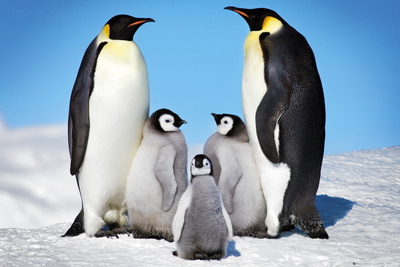
\includegraphics[scale=.50]{figures/Penguins.jpg}
\caption{TAMU figure}
\label{fig:tamu-fig5}
\end{figure}

%%%%%%%%%%%%%%%%%%%%%%%%%%%%%%%%%%%%%%%%%%%%%%%%%%%
%
%  New template code for TAMU Theses and Dissertations starting Fall 2016.
%
%
%  Author: Sean Zachary Roberson 
%	 Version 3.16.09 
%  Last updated 9/12/2016
%
%%%%%%%%%%%%%%%%%%%%%%%%%%%%%%%%%%%%%%%%%%%%%%%%%%%

%%%%%%%%%%%%%%%%%%%%%%%%%%%%%%%%%%%%%%%%%%%%%%%%%%%%%%%%%%%%%%%%%%%%%%
%%                           APPENDIX B
%%%%%%%%%%%%%%%%%%%%%%%%%%%%%%%%%%%%%%%%%%%%%%%%%%%%%%%%%%%%%%%%%%%%%

\chapter{\uppercase {A Second Appendix Whose Title Is Much Longer Than The First}}

Text for the Appendix follows.

\begin{figure}[h]
\centering
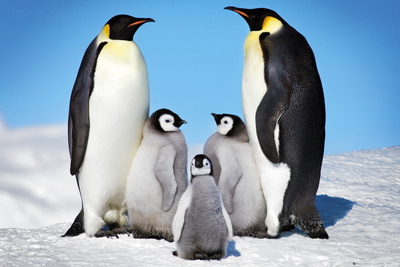
\includegraphics[scale=.50]{figures/Penguins.jpg}
\caption{Another TAMU figure.}
\label{fig:tamu-fig6}
\end{figure}

\section{Appendix Section}

\section{Second Appendix Section}


\pagebreak{}

\end{appendices}

\end{document}
